%!TEX encoding = UTF-8 Unicode
\documentclass[onecolumn,12pt]{book}\usepackage[]{graphicx}\usepackage[]{color}
%% maxwidth is the original width if it is less than linewidth
%% otherwise use linewidth (to make sure the graphics do not exceed the margin)
\makeatletter
\def\maxwidth{ %
  \ifdim\Gin@nat@width>\linewidth
    \linewidth
  \else
    \Gin@nat@width
  \fi
}
\makeatother

\definecolor{fgcolor}{rgb}{0.345, 0.345, 0.345}
\newcommand{\hlnum}[1]{\textcolor[rgb]{0.686,0.059,0.569}{#1}}%
\newcommand{\hlstr}[1]{\textcolor[rgb]{0.192,0.494,0.8}{#1}}%
\newcommand{\hlcom}[1]{\textcolor[rgb]{0.678,0.584,0.686}{\textit{#1}}}%
\newcommand{\hlopt}[1]{\textcolor[rgb]{0,0,0}{#1}}%
\newcommand{\hlstd}[1]{\textcolor[rgb]{0.345,0.345,0.345}{#1}}%
\newcommand{\hlkwa}[1]{\textcolor[rgb]{0.161,0.373,0.58}{\textbf{#1}}}%
\newcommand{\hlkwb}[1]{\textcolor[rgb]{0.69,0.353,0.396}{#1}}%
\newcommand{\hlkwc}[1]{\textcolor[rgb]{0.333,0.667,0.333}{#1}}%
\newcommand{\hlkwd}[1]{\textcolor[rgb]{0.737,0.353,0.396}{\textbf{#1}}}%

\usepackage{framed}
\makeatletter
\newenvironment{kframe}{%
 \def\at@end@of@kframe{}%
 \ifinner\ifhmode%
  \def\at@end@of@kframe{\end{minipage}}%
  \begin{minipage}{\columnwidth}%
 \fi\fi%
 \def\FrameCommand##1{\hskip\@totalleftmargin \hskip-\fboxsep
 \colorbox{shadecolor}{##1}\hskip-\fboxsep
     % There is no \\@totalrightmargin, so:
     \hskip-\linewidth \hskip-\@totalleftmargin \hskip\columnwidth}%
 \MakeFramed {\advance\hsize-\width
   \@totalleftmargin\z@ \linewidth\hsize
   \@setminipage}}%
 {\par\unskip\endMakeFramed%
 \at@end@of@kframe}
\makeatother

\definecolor{shadecolor}{rgb}{.97, .97, .97}
\definecolor{messagecolor}{rgb}{0, 0, 0}
\definecolor{warningcolor}{rgb}{1, 0, 1}
\definecolor{errorcolor}{rgb}{1, 0, 0}
\newenvironment{knitrout}{}{} % an empty environment to be redefined in TeX

\usepackage{alltt}
\usepackage[english,italian]{babel}
\usepackage{inconsolata}
%\renewcommand*\familydefault{\ttdefault} %% Only if the base font of the document is to be typewriter style
\usepackage[T1]{fontenc}

\usepackage{a4wide,Sweave,url}
\usepackage{verbatim}
\usepackage{makeidx}
\usepackage{babelbib}
\usepackage{float}
\usepackage{fancyhdr}
\usepackage[T1]{fontenc}
\usepackage[utf8]{inputenc}
\usepackage{framed}
\usepackage{lipsum}
\usepackage[dvipsnames]{color}
\definecolor{shadecolor}{rgb}{0.9,0.9,0.9}
\usepackage{graphicx}
\usepackage{fancyvrb}
\usepackage{amsmath}

\usepackage{hyperref}
\newenvironment{question}{\item \textbf{Esercizio}\newline}{}
\newenvironment{solution}{\textbf{Soluzione}\newline}{}
\newenvironment{answerlist}{\renewcommand{\labelenumi}{(\alph{enumi})}\begin{enumerate}}{\end{enumerate}}
\definecolor{grigetto}{rgb}{0.9,0.9,0.9}
 
\DefineVerbatimEnvironment{Sinput}{Verbatim} {xleftmargin=2em} \DefineVerbatimEnvironment{Soutput}{Verbatim}{xleftmargin=2em} \DefineVerbatimEnvironment{Scode}{Verbatim}{xleftmargin=2em} \fvset{listparameters={\setlength{\topsep}{0pt}}} \renewenvironment{Schunk}{\small\vspace{\topsep}}{\vspace{\topsep}\normalsize}
\lhead[\thepage]{\today}
%\usepackage{draftwatermark}
\usepackage{wrapfig}
\usepackage{listings}
\pagestyle{fancy}
\newcounter{fnotes}\setcounter{fnotes}{1}
\newcounter{Raction}\setcounter{Raction}{1}
\newcommand{\varia}[1]{\textsl{\textsf{#1}}}
\newcommand{\mytilde}{$\sim$}
\newcommand{\maurizio}[1]{\color{red}#1 \color{black}}
\newcommand{\federico}[1]{\color{green}#1 \color{black}}
 %\newenvironment{question}{\item \textbf{Problema}\newline}{}
%\newenvironment{solution}{\textbf{Soluzione}\newline}{}
%\DefineVerbatimEnvironment{Sinput}{Verbatim} {xleftmargin=2em,
                                            %  frame=single}
\DefineVerbatimEnvironment{Soutput}{Verbatim}{xleftmargin=2em,   frame=single}
 \newenvironment{ese} [1]{\vskip10pt
%\begin{center}
%\begin{minipage}{12cm}
 \markright{\today}
\definecolor{grigetto}{rgb}{0.9,0.9,0.9}
\colorbox{grigetto}{\parbox{\linewidth}{#1}}}
                          {
                         % \end{minipage}
                          %\end{center}
                          \medskip}
 \newcommand{\virgolette}{\selectlanguage{english}\texttt{"}\selectlanguage{italian}}
 \frontmatter\title{Matematica e Statistica con \textsf{R}}
\author{Federico Comoglio e  Maurizio Rinaldi}
\markright{\today}
\lhead{\today}
\renewcommand{\chaptermark}[1]{%
 \markboth{\chaptername
 \ \thechapter.\ #1}{}}
%\renewcommand{\sectionmark}[1]{%
% \markboth{\sectionname
% \ \thesection.\ #1}{}}
\newcommand{\rst}{\textsf{RStudio}~}
\newcommand{\rpr}{\textsf{R}~}
\makeindex
\IfFileExists{upquote.sty}{\usepackage{upquote}}{}
\begin{document}



\setkeys{Gin}{width=0.7\textwidth}



\markright{\today}
\thispagestyle{empty}
\maketitle
\newpage
\thispagestyle{empty}
\tableofcontents
\newpage
\thispagestyle{empty}
 \mainmatter

\chapter{Introduzione}
\begin{knitrout}
\definecolor{shadecolor}{rgb}{0.969, 0.969, 0.969}\color{fgcolor}\begin{kframe}
\begin{alltt}
\hlstd{knit_hooks}\hlopt{$}\hlkwd{set}\hlstd{(}\hlkwc{pars} \hlstd{=} \hlkwa{function}\hlstd{(}\hlkwc{before}\hlstd{,} \hlkwc{options}\hlstd{,} \hlkwc{envir}\hlstd{) \{}
  \hlkwa{if} \hlstd{(before) graphics}\hlopt{::}\hlkwd{par}\hlstd{(options}\hlopt{$}\hlstd{pars)}
\hlstd{\})}
\end{alltt}
\end{kframe}
\end{knitrout}

\begin{knitrout}
\definecolor{shadecolor}{rgb}{0.969, 0.969, 0.969}\color{fgcolor}\begin{kframe}
\begin{alltt}
\hlkwd{plot}\hlstd{(mtcars[,} \hlnum{1}\hlopt{:}\hlnum{2}\hlstd{])}
\end{alltt}


{\ttfamily\noindent\bfseries\color{errorcolor}{\#\# Error in getMetricsFromLatex(TeXMetrics, verbose = verbose): \\\#\# TeX was unable to calculate metrics for the following string\\\#\# or character:\\\#\# \\\#\# 	m\\\#\# \\\#\# Common reasons for failure include:\\\#\#\ \  * The string contains a character which is special to LaTeX unless\\\#\#\ \ \ \  escaped properly, such as \% or \$.\\\#\#\ \  * The string makes use of LaTeX commands provided by a package and\\\#\#\ \ \ \  the tikzDevice was not told to load the package.\\\#\# \\\#\# The contents of the LaTeX log of the aborted run have been printed above,\\\#\# it may contain additional details as to why the metric calculation failed.}}\end{kframe}

{\centering 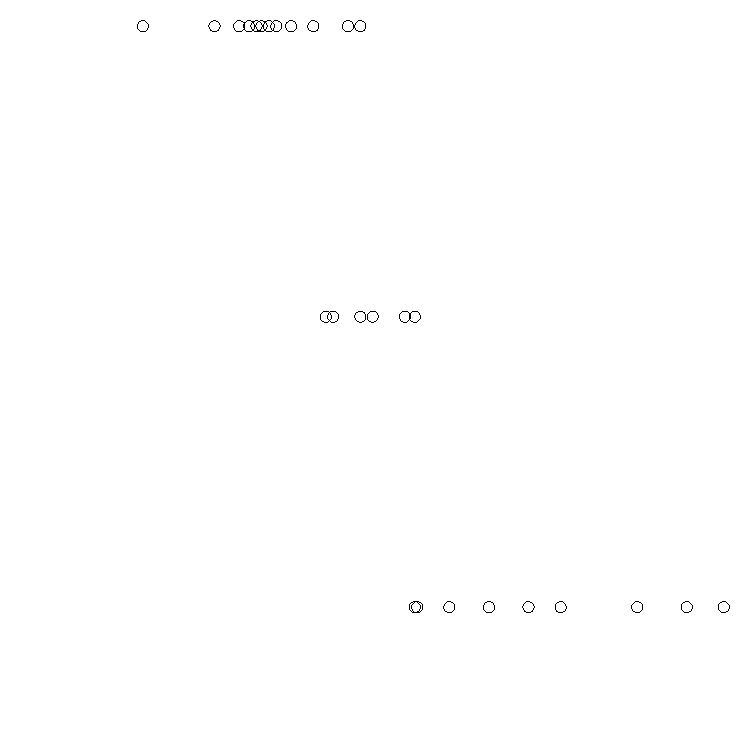
\includegraphics[width=\maxwidth]{figure/graphics-use-pars-1} 

}



\end{knitrout}
Per accedere ai dati richiesti in questa parte occorre caricare il pacchetto allegato \texttt{libroR}. Per farlo conviene scaricare il file \texttt{libroR$\_0$.0.tgz}  sul proprio computer e  selezionare il menu \texttt{Install}
\begin{center}\begin{figure}[H]
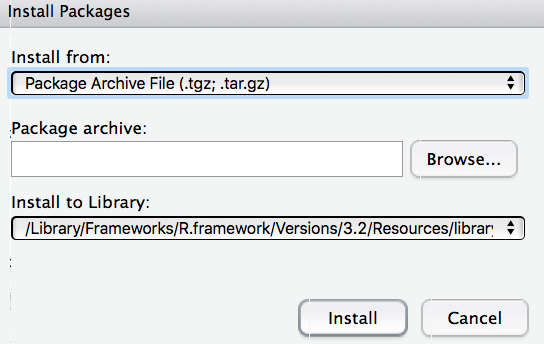
\includegraphics[width=0.4\textwidth]{../grafici/installlibro.png}
\caption{Procedura di installazione del pacchetto}
\label{fig::rlibroinstall} \end{figure}
\end{center}
Il file viene poi localizzato usando \texttt{Browse..}. \\
Alternativamente si pu\`o utilizzare direttamente il comando

\begin{knitrout}
\definecolor{shadecolor}{rgb}{0.969, 0.969, 0.969}\color{fgcolor}\begin{kframe}
\begin{alltt}
\hlkwd{install.packages}\hlstd{(}\hlstr{"libroR_0.0.tgz"}\hlstd{,} \hlkwc{repos} \hlstd{=} \hlkwa{NULL}\hlstd{,} \hlkwc{type} \hlstd{= .Platform}\hlopt{$}\hlstd{pkgType)}
\end{alltt}
\end{kframe}
\end{knitrout}
a patto di impostare la \emph{working directory} precisamente dove si trova il file.
Il pacchetto va poi successivamente caricato con il comando
\begin{knitrout}
\definecolor{shadecolor}{rgb}{0.969, 0.969, 0.969}\color{fgcolor}\begin{kframe}
\begin{alltt}
\hlkwd{library}\hlstd{(}\hlstr{"libroR"}\hlstd{)}
\end{alltt}
\end{kframe}
\end{knitrout}

Precisiamo inoltre che questa \`e una versione assolutamente preliminare.
\chapter{Strutture di dati}

 
Per visualizzare un oggetto di \textsf{R} si pu\`o usare il comando \texttt{print} o il comando \texttt{cat} che fornisce spesso un risultato migliore. \texttt{str} visualizza la struttura di un oggetto mentre \texttt{head} o \texttt{tail} ne visualizzano l'inizio o la fine.


\section{I diversi  tipi di vettori}
\subsection{Vettori di caratteri/stringhe}
Una stringa\index{stringa} di testo \`e una collezione di caratteri; in genere, una stringa \`e resa riconoscibile dall'essere racchiusa tra virgolette.
\subsubsection{Operare con le stringhe}
Oltre alle virgolette, vi sono numerosi altri caratteri speciali che possono apparire in una stringa.
I pi\`u comuni sono ``\texttt{\textbackslash t}'' per \texttt{TAB}, `` \texttt{\textbackslash n}'' per una nuova linea e ``\texttt{\textbackslash }'' per un singolo {\it backslash}.
Quest'ultimo carattere \`e un carattere di \emph{escape} e consente una lettura diversa di quanto lo segue.  Per esempio
\begin{knitrout}
\definecolor{shadecolor}{rgb}{0.969, 0.969, 0.969}\color{fgcolor}\begin{kframe}
\begin{alltt}
\hlkwd{cat}\hlstd{(}\hlstr{"\textbackslash{}"sin\textbackslash{}""}\hlstd{)}
\end{alltt}
\begin{verbatim}
## "sin"
\end{verbatim}
\begin{alltt}
\hlkwd{nchar}\hlstd{(}\hlstr{"\textbackslash{}"sin\textbackslash{}""}\hlstd{)}
\end{alltt}
\begin{verbatim}
## [1] 5
\end{verbatim}
\begin{alltt}
\hlkwd{cat}\hlstd{(}\hlstr{"\textbackslash{}\textbackslash{}"}\hlstd{)}
\end{alltt}
\begin{verbatim}
## \
\end{verbatim}
\begin{alltt}
\hlkwd{cat}\hlstd{(}\hlstr{"ora a capo\textbackslash{}nsono a capo?"}\hlstd{)}
\end{alltt}
\begin{verbatim}
## ora a capo
## sono a capo?
\end{verbatim}
\begin{alltt}
\hlkwd{cat}\hlstd{(}\hlstr{"ora spazio\textbackslash{}triprendo"}\hlstd{)}
\end{alltt}
\begin{verbatim}
## ora spazio	riprendo
\end{verbatim}
\end{kframe}
\end{knitrout}
La funzione \texttt{nchar}, \index{\texttt{nchar}} che conta il numero di caratteri di una stringa, non includer\`a quindi il carattere di \emph{escape}\index{\emph{escape}} nel totale dei caratteri. Ad esempio:
\begin{knitrout}
\definecolor{shadecolor}{rgb}{0.969, 0.969, 0.969}\color{fgcolor}\begin{kframe}
\begin{alltt}
\hlstr{"Tab\textbackslash{}t"}
\end{alltt}
\begin{verbatim}
## [1] "Tab\t"
\end{verbatim}
\begin{alltt}
\hlkwd{cat}\hlstd{(}\hlstr{"Tab\textbackslash{}t"}\hlstd{)}
\end{alltt}
\begin{verbatim}
## Tab	
\end{verbatim}
\begin{alltt}
\hlkwd{nchar}\hlstd{(}\hlstr{"Tab\textbackslash{}t"}\hlstd{)}
\end{alltt}
\begin{verbatim}
## [1] 4
\end{verbatim}
\end{kframe}
\end{knitrout}



Succede spesso di dover lavorare in modo automatico con stringhe di testo, anche nello scrivere indirizzi di rete o cartelle di lavoro. In  \textsf{R} diversi comandi consentono la  generazione, manipolazione e stampa di una o pi\`u stringhe di testo\footnote{Per un  uso pi\`u specifico si pu\`o consultare il pacchetto \texttt{biostrings}.}. Consideriamo inizialmente una singola frase.
%codechunk
\begin{knitrout}
\definecolor{shadecolor}{rgb}{0.969, 0.969, 0.969}\color{fgcolor}\begin{kframe}
\begin{alltt}
\hlstd{x}\hlkwb{=}\hlstr{"lavorare con le stringhe"}
\end{alltt}
\end{kframe}
\end{knitrout}
Possiamo verificarne la classe e determinare il numero di caratteri di \texttt{x}
%codechunk
\begin{knitrout}
\definecolor{shadecolor}{rgb}{0.969, 0.969, 0.969}\color{fgcolor}\begin{kframe}
\begin{alltt}
\hlkwd{class}\hlstd{(x)}
\end{alltt}
\begin{verbatim}
## [1] "character"
\end{verbatim}
\begin{alltt}
\hlkwd{nchar}\hlstd{(x)}
\end{alltt}
\begin{verbatim}
## [1] 24
\end{verbatim}
\end{kframe}
\end{knitrout}
e anche considerare sottostringhe
%codechunk
\begin{knitrout}
\definecolor{shadecolor}{rgb}{0.969, 0.969, 0.969}\color{fgcolor}\begin{kframe}
\begin{alltt}
\hlkwd{substr}\hlstd{(x,}\hlnum{3}\hlstd{,}\hlnum{8}\hlstd{)}
\end{alltt}
\begin{verbatim}
## [1] "vorare"
\end{verbatim}
\end{kframe}
\end{knitrout}
o  abbreviazioni ottenibili con il comando \texttt{abbreviate} \index{\texttt{abbreviate}}
%codechunk
\begin{knitrout}
\definecolor{shadecolor}{rgb}{0.969, 0.969, 0.969}\color{fgcolor}\begin{kframe}
\begin{alltt}
\hlkwd{abbreviate}\hlstd{(}\hlstr{"Mario Rossi"}\hlstd{,}\hlnum{4}\hlstd{)}
\end{alltt}
\begin{verbatim}
## Mario Rossi 
##      "MrRs"
\end{verbatim}
\end{kframe}
\end{knitrout}

Certi oggetti possono essere convertiti a stringhe: per esempio il numero 2 pu\`o essere visto come una stringa e riconvertito a numero.
%codechunk
\begin{knitrout}
\definecolor{shadecolor}{rgb}{0.969, 0.969, 0.969}\color{fgcolor}\begin{kframe}
\begin{alltt}
\hlstd{i}\hlkwb{=}\hlnum{2}\hlstd{;}\hlkwd{toString}\hlstd{(i)}
\end{alltt}
\begin{verbatim}
## [1] "2"
\end{verbatim}
\begin{alltt}
\hlkwd{as.numeric}\hlstd{(}\hlkwd{toString}\hlstd{(i))}
\end{alltt}
\begin{verbatim}
## [1] 2
\end{verbatim}
\end{kframe}
\end{knitrout}
Alcune stringhe molto frequenti sono le lettere \index{\texttt{letters}}\index{\texttt{LETTERS}} dell'alfabeto, maiuscole o minuscole
%codechunk
\begin{knitrout}
\definecolor{shadecolor}{rgb}{0.969, 0.969, 0.969}\color{fgcolor}\begin{kframe}
\begin{alltt}
\hlstd{letters[}\hlnum{1}\hlopt{:}\hlnum{10}\hlstd{]}
\end{alltt}
\begin{verbatim}
##  [1] "a" "b" "c" "d" "e" "f" "g" "h" "i" "j"
\end{verbatim}
\begin{alltt}
\hlstd{LETTERS[}\hlnum{1}\hlopt{:}\hlnum{10}\hlstd{]}
\end{alltt}
\begin{verbatim}
##  [1] "A" "B" "C" "D" "E" "F" "G" "H" "I" "J"
\end{verbatim}
\end{kframe}
\end{knitrout}
o i mesi dell'anno (per esempio abbreviati in inglese)\index{\texttt{month.abb}}
%codechunk

\begin{knitrout}
\definecolor{shadecolor}{rgb}{0.969, 0.969, 0.969}\color{fgcolor}\begin{kframe}
\begin{alltt}
\hlstd{month.abb}
\end{alltt}
\begin{verbatim}
##  [1] "Jan" "Feb" "Mar" "Apr" "May" "Jun" "Jul" "Aug" "Sep"
## [10] "Oct" "Nov" "Dec"
\end{verbatim}
\end{kframe}
\end{knitrout}
Le stringhe possono poi essere ``incollate'' con il comando\index{\texttt{paste}}
%codechunk
\begin{knitrout}
\definecolor{shadecolor}{rgb}{0.969, 0.969, 0.969}\color{fgcolor}\begin{kframe}
\begin{alltt}
\hlkwd{paste}\hlstd{(}\hlstr{"a"}\hlstd{,}\hlstr{"b"}\hlstd{,}\hlkwc{sep}\hlstd{=}\hlstr{""}\hlstd{)}
\end{alltt}
\end{kframe}
\end{knitrout}
dove \texttt{sep}  indica il separatore usato.
E tutto insieme
%codechunk


\begin{knitrout}
\definecolor{shadecolor}{rgb}{0.969, 0.969, 0.969}\color{fgcolor}\begin{kframe}
\begin{alltt}
\hlkwa{for} \hlstd{(i} \hlkwa{in} \hlnum{1}\hlopt{:}\hlnum{5}\hlstd{)} \hlkwd{cat}\hlstd{(}\hlkwd{paste}\hlstd{(}\hlstr{"a"}\hlstd{,}\hlkwd{toString}\hlstd{(i),}\hlstr{"\textbackslash{}t"}\hlstd{,}\hlkwc{sep}\hlstd{=}\hlstr{""}\hlstd{))}
\end{alltt}
\begin{verbatim}
## a1	a2	a3	a4	a5	
\end{verbatim}
\end{kframe}
\end{knitrout}
Il comando pu\`o anche essere utilizzato su vettori.
Per esempio
%codechunk
\begin{knitrout}
\definecolor{shadecolor}{rgb}{0.969, 0.969, 0.969}\color{fgcolor}\begin{kframe}
\begin{alltt}
\hlkwd{paste}\hlstd{(letters[}\hlnum{1}\hlopt{:}\hlnum{10}\hlstd{],}\hlnum{1}\hlopt{:}\hlnum{10}\hlstd{,}\hlkwc{sep}\hlstd{=}\hlstr{""}\hlstd{)}
\end{alltt}
\begin{verbatim}
##  [1] "a1"  "b2"  "c3"  "d4"  "e5"  "f6"  "g7"  "h8"  "i9" 
## [10] "j10"
\end{verbatim}
\end{kframe}
\end{knitrout}
La \textit{recycling rule} continua a valere
%codechunk

\begin{knitrout}
\definecolor{shadecolor}{rgb}{0.969, 0.969, 0.969}\color{fgcolor}\begin{kframe}
\begin{alltt}
\hlkwd{paste}\hlstd{(letters[}\hlnum{1}\hlopt{:}\hlnum{3}\hlstd{],}\hlnum{1}\hlopt{:}\hlnum{10}\hlstd{,}\hlkwc{sep}\hlstd{=}\hlstr{""}\hlstd{)}
\end{alltt}
\begin{verbatim}
##  [1] "a1"  "b2"  "c3"  "a4"  "b5"  "c6"  "a7"  "b8"  "c9" 
## [10] "a10"
\end{verbatim}
\begin{alltt}
\hlkwd{paste}\hlstd{(letters[}\hlnum{1}\hlopt{:}\hlnum{3}\hlstd{],}\hlnum{1}\hlopt{:}\hlnum{12}\hlstd{,}\hlkwc{sep}\hlstd{=}\hlstr{""}\hlstd{)}
\end{alltt}
\begin{verbatim}
##  [1] "a1"  "b2"  "c3"  "a4"  "b5"  "c6"  "a7"  "b8"  "c9" 
## [10] "a10" "b11" "c12"
\end{verbatim}
\end{kframe}
\end{knitrout}
e giocando con \texttt{rep} si possono ottenere diverse combinazioni.
\begin{knitrout}
\definecolor{shadecolor}{rgb}{0.969, 0.969, 0.969}\color{fgcolor}\begin{kframe}
\begin{alltt}
\hlkwd{paste}\hlstd{(}\hlkwd{rep}\hlstd{(letters[}\hlnum{1}\hlopt{:}\hlnum{3}\hlstd{],}\hlkwc{each}\hlstd{=}\hlnum{5}\hlstd{),}\hlnum{1}\hlopt{:}\hlnum{15}\hlstd{,}\hlkwc{sep}\hlstd{=}\hlstr{""}\hlstd{)}
\end{alltt}
\begin{verbatim}
##  [1] "a1"  "a2"  "a3"  "a4"  "a5"  "b6"  "b7"  "b8"  "b9" 
## [10] "b10" "c11" "c12" "c13" "c14" "c15"
\end{verbatim}
\begin{alltt}
\hlkwd{paste}\hlstd{(}\hlkwd{rep}\hlstd{(letters[}\hlnum{1}\hlopt{:}\hlnum{3}\hlstd{],}\hlkwc{ntimes}\hlstd{=}\hlnum{5}\hlstd{),}\hlnum{1}\hlopt{:}\hlnum{15}\hlstd{,}\hlkwc{sep}\hlstd{=}\hlstr{""}\hlstd{)}
\end{alltt}
\begin{verbatim}
##  [1] "a1"  "b2"  "c3"  "a4"  "b5"  "c6"  "a7"  "b8"  "c9" 
## [10] "a10" "b11" "c12" "a13" "b14" "c15"
\end{verbatim}
\end{kframe}
\end{knitrout}
Con l'opzione \texttt{collapse="x"} le stringhe vengono unite con separatore la stringa "x".


\begin{knitrout}
\definecolor{shadecolor}{rgb}{0.969, 0.969, 0.969}\color{fgcolor}\begin{kframe}
\begin{alltt}
\hlkwd{paste}\hlstd{(}\hlkwd{c}\hlstd{(}\hlstr{"X"}\hlstd{,} \hlstr{"Y"}\hlstd{),} \hlnum{1}\hlopt{:}\hlnum{4}\hlstd{,} \hlkwc{sep} \hlstd{=} \hlstr{"-"}\hlstd{,} \hlkwc{collapse} \hlstd{=} \hlstr{"--"}\hlstd{)}
\end{alltt}
\begin{verbatim}
## [1] "X-1--Y-2--X-3--Y-4"
\end{verbatim}
\end{kframe}
\end{knitrout}
Si noti il separatore - dell'operazione \texttt{paste} e  - - dell'operazione \texttt{collapse}.

 \begin{shaded}
 \begin{enumerate}
 \item{} Inserisci il tuo cognome in una variabile `cognome' ed il tuo nome in una variabile 'nome'. Crea una terza variabile 'nomecognome' che contenga entrambi separati da un TAB. Stampa a console la scritta "Good job" seguita dal valore di nomecognome.
  \item{} Creare un elenco che contenga mesi e anno dal 2001 al 2010 nel seguente formato "tre lettere iniziali del mese-anno".
 \item{} Costruire una tabella che contenga tutte le parole di 2 lettere.
\item{}
Si consideri
\begin{knitrout}
\definecolor{shadecolor}{rgb}{0.969, 0.969, 0.969}\color{fgcolor}\begin{kframe}
\begin{alltt}
\hlkwd{paste}\hlstd{(letters[}\hlnum{1}\hlopt{:}\hlnum{7}\hlstd{],}\hlnum{1}\hlopt{:}\hlnum{7}\hlstd{,}\hlkwc{sep}\hlstd{=}\hlstr{"="}\hlstd{)}
\end{alltt}
\end{kframe}
\end{knitrout}
Estendere la corrispondenza a tutto l'alfabeto.
\item Creare un elenco in cui a ciascun mese corrisponda il suo numero (a partire da gennaio).
\item Creare un elenco con nomi i mesi e valori il numero di giorni di ciascun mese.
\item Scrivere un elenco di 5 persone con le relative date di nascita nel formato anno-mese-giorno.
 \end{enumerate}
 \end{shaded}
\subsection{Vettori logici}
I valori logici in R sono i valori \texttt{TRUE} e \texttt{FALSE} e corrispondono alla veridicit\`a di un'affermazione.
Per esempio
\begin{knitrout}
\definecolor{shadecolor}{rgb}{0.969, 0.969, 0.969}\color{fgcolor}\begin{kframe}
\begin{alltt}
\hlnum{1}\hlopt{:}\hlnum{10} \hlopt{>} \hlnum{4}
\end{alltt}
\begin{verbatim}
##  [1] FALSE FALSE FALSE FALSE  TRUE  TRUE  TRUE  TRUE  TRUE
## [10]  TRUE
\end{verbatim}
\end{kframe}
\end{knitrout}
Ci fornisce simultaneamente i valori dei 10 confronti.
\section{Vettori numerici e operazioni di aritmetica modulare}
\begin{knitrout}
\definecolor{shadecolor}{rgb}{0.969, 0.969, 0.969}\color{fgcolor}\begin{kframe}
\begin{alltt}
\hlnum{1}\hlopt{:}\hlnum{10}
\end{alltt}
\begin{verbatim}
##  [1]  1  2  3  4  5  6  7  8  9 10
\end{verbatim}
\end{kframe}
\end{knitrout}
\begin{knitrout}
\definecolor{shadecolor}{rgb}{0.969, 0.969, 0.969}\color{fgcolor}\begin{kframe}
\begin{alltt}
\hlstd{resto}\hlkwb{=}\hlstd{(}\hlnum{1}\hlopt{:}\hlnum{10}\hlstd{)}\hlopt\hlnum{4}
\hlstd{resto}
\end{alltt}
\begin{verbatim}
##  [1] 1 2 3 0 1 2 3 0 1 2
\end{verbatim}
\begin{alltt}
\hlstd{quoziente}\hlkwb{=}\hlstd{(}\hlnum{1}\hlopt{:}\hlnum{10}\hlstd{)}\hlopt\hlnum{4}
\hlstd{quoziente}
\end{alltt}
\begin{verbatim}
##  [1] 0 0 0 1 1 1 1 2 2 2
\end{verbatim}
\begin{alltt}
\hlstd{resto}\hlopt{+}\hlnum{4}\hlopt{*}\hlstd{quoziente}
\end{alltt}
\begin{verbatim}
##  [1]  1  2  3  4  5  6  7  8  9 10
\end{verbatim}
\end{kframe}
\end{knitrout}
\section{Matrici}

Assegnati $n\times m$ ingressi possiamo costruire una matrice (ossia una tabella) con $n$ righe e $m$ colonne. Occorre solo riempire la matrice per righe o per colonne.
Ad esempio:
%code chunk
\begin{knitrout}
\definecolor{shadecolor}{rgb}{0.969, 0.969, 0.969}\color{fgcolor}\begin{kframe}
\begin{alltt}
\hlstd{a}\hlkwb{<-}\hlkwd{matrix}\hlstd{(letters[}\hlnum{1}\hlopt{:}\hlnum{12}\hlstd{],}\hlkwc{nrow}\hlstd{=}\hlnum{3}\hlstd{,}\hlkwc{ncol}\hlstd{=}\hlnum{4}\hlstd{)}
\hlstd{a}
\end{alltt}
\begin{verbatim}
##      [,1] [,2] [,3] [,4]
## [1,] "a"  "d"  "g"  "j" 
## [2,] "b"  "e"  "h"  "k" 
## [3,] "c"  "f"  "i"  "l"
\end{verbatim}
\begin{alltt}
\hlkwd{class}\hlstd{(a)}
\end{alltt}
\begin{verbatim}
## [1] "matrix"
\end{verbatim}
\end{kframe}
\end{knitrout}
Se i parametri hanno natura diversa vengono resi uniformi
%code chunk
\begin{knitrout}
\definecolor{shadecolor}{rgb}{0.969, 0.969, 0.969}\color{fgcolor}\begin{kframe}
\begin{alltt}
\hlstd{a}\hlkwb{<-}\hlkwd{matrix}\hlstd{(}\hlkwd{c}\hlstd{(}\hlnum{1}\hlopt{:}\hlnum{6}\hlstd{,letters[}\hlnum{1}\hlopt{:}\hlnum{6}\hlstd{]),}\hlkwc{nrow}\hlstd{=}\hlnum{3}\hlstd{,}\hlkwc{ncol}\hlstd{=}\hlnum{4}\hlstd{);a}
\end{alltt}
\begin{verbatim}
##      [,1] [,2] [,3] [,4]
## [1,] "1"  "4"  "a"  "d" 
## [2,] "2"  "5"  "b"  "e" 
## [3,] "3"  "6"  "c"  "f"
\end{verbatim}
\end{kframe}
\end{knitrout}
Con il parametro \texttt{byrow=T} il riempimento avviene per righe, anzich\`e per colonne.
%code chunk
\begin{knitrout}
\definecolor{shadecolor}{rgb}{0.969, 0.969, 0.969}\color{fgcolor}\begin{kframe}
\begin{alltt}
 \hlstd{a}\hlkwb{<-}\hlkwd{matrix}\hlstd{(}\hlnum{1}\hlopt{:}\hlnum{12}\hlstd{,}\hlkwc{nrow}\hlstd{=}\hlnum{3}\hlstd{,}\hlkwc{ncol}\hlstd{=}\hlnum{4}\hlstd{,}\hlkwc{byrow}\hlstd{=T)}
 \hlstd{a}
\end{alltt}
\begin{verbatim}
##      [,1] [,2] [,3] [,4]
## [1,]    1    2    3    4
## [2,]    5    6    7    8
## [3,]    9   10   11   12
\end{verbatim}
\end{kframe}
\end{knitrout}
Se i numeri sono insufficienti vengono \emph {riciclati}
%code chunk
\begin{knitrout}
\definecolor{shadecolor}{rgb}{0.969, 0.969, 0.969}\color{fgcolor}\begin{kframe}
\begin{alltt}
\hlstd{a}\hlkwb{<-}\hlkwd{matrix}\hlstd{(}\hlnum{1}\hlopt{:}\hlnum{4}\hlstd{,}\hlkwc{nrow}\hlstd{=}\hlnum{3}\hlstd{,}\hlkwc{ncol}\hlstd{=}\hlnum{4}\hlstd{)}
\hlstd{a}
\end{alltt}
\begin{verbatim}
##      [,1] [,2] [,3] [,4]
## [1,]    1    4    3    2
## [2,]    2    1    4    3
## [3,]    3    2    1    4
\end{verbatim}
\end{kframe}
\end{knitrout}
in modo pacifico se sono un sottomultiplo della dimensione della matrice o con qualche
\texttt{warning} altrimenti.
%code chunk
\begin{knitrout}
\definecolor{shadecolor}{rgb}{0.969, 0.969, 0.969}\color{fgcolor}\begin{kframe}
\begin{alltt}
\hlstd{a}\hlkwb{<-}\hlkwd{matrix}\hlstd{(}\hlnum{2}\hlstd{,}\hlkwc{nrow}\hlstd{=}\hlnum{3}\hlstd{,}\hlkwc{ncol}\hlstd{=}\hlnum{4}\hlstd{)}
\hlstd{a}
\end{alltt}
\end{kframe}
\end{knitrout}
Si possono anche definire gli ingressi attraverso opportune funzioni
%code chunk

\begin{knitrout}
\definecolor{shadecolor}{rgb}{0.969, 0.969, 0.969}\color{fgcolor}\begin{kframe}
\begin{alltt}
\hlkwa{for}\hlstd{(j} \hlkwa{in} \hlstd{(}\hlnum{1}\hlopt{:}\hlnum{4}\hlstd{))} \hlkwa{for}\hlstd{(i} \hlkwa{in} \hlstd{(}\hlnum{1}\hlopt{:}\hlnum{3}\hlstd{))  a[i,j]}\hlkwb{<-}\hlstd{i}\hlopt{^}\hlnum{2}\hlopt{+}\hlstd{j}
\end{alltt}
\end{kframe}
\end{knitrout}
Per assegnare nomi alle  righe e alle colonne:\index{\texttt{colnames}} \index{\texttt{rownames}}
\begin{eqnarray*}
 \texttt{colnames}(\varia{matrice})=\texttt{c}(\virgolette \varia{  nome}_1\virgolette,\\
\virgolette \varia{nome}_2\virgolette,\ldots,\virgolette \varia{nome}_n\virgolette )\\
 \texttt{rownames}(\varia{matrice})=\texttt{c}(\virgolette \varia{nome}_1\virgolette,\\
\virgolette \varia{nome}_2\virgolette,\ldots,\virgolette \varia{nome}_n\virgolette )
\end{eqnarray*}
\begin{knitrout}
\definecolor{shadecolor}{rgb}{0.969, 0.969, 0.969}\color{fgcolor}\begin{kframe}
\begin{alltt}
\hlkwd{colnames}\hlstd{(a)}\hlkwb{=}\hlkwd{c}\hlstd{(}\hlstr{"c1"}\hlstd{,}\hlstr{"c2"}\hlstd{,}\hlstr{"c3"}\hlstd{,}\hlstr{"c4"}\hlstd{)}
\hlkwd{rownames}\hlstd{(a)}\hlkwb{=}\hlkwd{c}\hlstd{(}\hlstr{"r1"}\hlstd{,}\hlstr{"r2"}\hlstd{,}\hlstr{"r3"}\hlstd{)}
\hlstd{a}
\end{alltt}
\begin{verbatim}
##    c1 c2 c3 c4
## r1  1  4  3  2
## r2  2  1  4  3
## r3  3  2  1  4
\end{verbatim}
\end{kframe}
\end{knitrout}
\subsubsection{Aggiungere righe o colonne}
Per aggiungere una o pi\`u righe (o colonne)
ad una matrice si possono usare i comandi (\texttt{rbind} e \texttt{cbind})
\begin{knitrout}
\definecolor{shadecolor}{rgb}{0.969, 0.969, 0.969}\color{fgcolor}\begin{kframe}
\begin{alltt}
\hlkwd{dim}\hlstd{(a)}
\end{alltt}
\begin{verbatim}
## [1] 3 4
\end{verbatim}
\begin{alltt}
\hlkwd{rbind}\hlstd{(a,letters[}\hlnum{1}\hlopt{:}\hlkwd{ncol}\hlstd{(a)])}
\end{alltt}
\begin{verbatim}
##    c1  c2  c3  c4 
## r1 "1" "4" "3" "2"
## r2 "2" "1" "4" "3"
## r3 "3" "2" "1" "4"
##    "a" "b" "c" "d"
\end{verbatim}
\begin{alltt}
\hlkwd{cbind}\hlstd{(a,letters[}\hlnum{1}\hlopt{:}\hlkwd{nrow}\hlstd{(a)])}
\end{alltt}
\begin{verbatim}
##    c1  c2  c3  c4     
## r1 "1" "4" "3" "2" "a"
## r2 "2" "1" "4" "3" "b"
## r3 "3" "2" "1" "4" "c"
\end{verbatim}
\end{kframe}
\end{knitrout}
Possiamo anche effettuare semplici operazioni, come somma degli elementi delle righe o delle colonne
\begin{knitrout}
\definecolor{shadecolor}{rgb}{0.969, 0.969, 0.969}\color{fgcolor}\begin{kframe}
\begin{alltt}
\hlkwd{colSums}\hlstd{(a)}
\end{alltt}
\begin{verbatim}
## c1 c2 c3 c4 
##  6  7  8  9
\end{verbatim}
\begin{alltt}
\hlkwd{rowSums}\hlstd{(a)}
\end{alltt}
\begin{verbatim}
## r1 r2 r3 
## 10 10 10
\end{verbatim}
\end{kframe}
\end{knitrout}

\subsection{Operazioni con le matrici}
\subsubsection{Trasposizione}
Per invertire righe e colonne di una matrice ossia per ottenere il trasposto \index{trasposto} di una matrice si usa il comando \texttt{t}(\texttt{matrice})\index{\texttt{t}, trasposto}
%code chunk
\begin{knitrout}
\definecolor{shadecolor}{rgb}{0.969, 0.969, 0.969}\color{fgcolor}\begin{kframe}
\begin{alltt}
\hlkwd{t}\hlstd{(a)}
\end{alltt}
\begin{verbatim}
##    r1 r2 r3
## c1  1  2  3
## c2  4  1  2
## c3  3  4  1
## c4  2  3  4
\end{verbatim}
\end{kframe}
\end{knitrout}
\subsubsection{Prodotto}
Per la  moltiplicazione di matrici (definita per ingressi numerici) si usa il simbolo \texttt{\%*\%}.
\index{\texttt{\%*\%}, prodotto di matrici}
 %code chunk
\begin{knitrout}
\definecolor{shadecolor}{rgb}{0.969, 0.969, 0.969}\color{fgcolor}\begin{kframe}
\begin{alltt}
\hlstd{b}\hlkwb{<-}\hlkwd{matrix}\hlstd{(}\hlnum{2}\hlstd{,}\hlkwc{nrow}\hlstd{=}\hlnum{3}\hlstd{,}\hlkwc{ncol}\hlstd{=}\hlnum{3}\hlstd{)}
\hlkwa{for}\hlstd{(j} \hlkwa{in} \hlstd{(}\hlnum{1}\hlopt{:}\hlnum{3}\hlstd{))}
\hlkwa{for}\hlstd{(i} \hlkwa{in} \hlstd{(}\hlnum{1}\hlopt{:}\hlnum{3}\hlstd{)) b[i,j]}\hlkwb{<-}\hlstd{i}\hlopt{+}\hlstd{j}\hlopt{+}\hlstd{i}\hlopt{^}\hlnum{2}
\hlstd{b}
\end{alltt}
\begin{verbatim}
##      [,1] [,2] [,3]
## [1,]    3    4    5
## [2,]    7    8    9
## [3,]   13   14   15
\end{verbatim}
\end{kframe}
\end{knitrout}
Non \`e infatti possibile moltiplicare una matrice 3x4 con una 3x3. Possiamo per\`o calcolare
%code chunk
\begin{knitrout}
\definecolor{shadecolor}{rgb}{0.969, 0.969, 0.969}\color{fgcolor}\begin{kframe}
\begin{alltt}
\hlstd{b}\hlopt\hlstd{a}
\end{alltt}
\begin{verbatim}
##      c1 c2  c3  c4
## [1,] 26 26  30  38
## [2,] 50 54  62  74
## [3,] 86 96 110 128
\end{verbatim}
\end{kframe}
\end{knitrout}
\subsubsection{Determinante} Il determinante di una matrice quadrata si ottiene con il comando
%\index{\texttt{det},determinante}
\begin{equation}\texttt{det} (\varia{matrice})\end{equation}
\begin{knitrout}
\definecolor{shadecolor}{rgb}{0.969, 0.969, 0.969}\color{fgcolor}\begin{kframe}
\begin{alltt}
\hlkwd{det}\hlstd{(b)}
\end{alltt}
\begin{verbatim}
## [1] 1.887379e-14
\end{verbatim}
\end{kframe}
\end{knitrout}

Si noti che se eseguendo i calcoli a mano si trovano in alcuni casi risultati diversi da quelli di {\textsf R}. Per esempio la matrice in esame ha determinante 0 e 0 ne \`e anche un autovalore.\index{autovalore}
\begin{shaded}
 \begin{enumerate}
 \item{}Creare una matrice $3\times 2$ che abbia come ingressi i primi 6 numeri pari. Estendere la matrice aggiungendo due colonne contenenti i primi 6 numeri dispari. Calcolare e stampare la somma per riga e la somma per colonna. Modifica la matrice cambiando di segno la prima riga. Moltiplicare la matrice  per 4.
 \end{enumerate}
 \end{shaded}
 \section{I \emph{dataframe}}

I \emph{dataframe} (in \rpr  \texttt{data.frame}) costituiscono in \rpr la classe di oggetti fondamentali per la collezione di dati per una susseguente analisi statistica.
Un \emph{dataframe}  \`e una collezione di vettori aventi egual lunghezza e allineati verticalmente. Un dataframe \`e diverso da una matrice in quanto le colonne sono vettori eventualmente di tipi diversi. Il comando generale per costruire \emph{dataframe} a partire da vettori o liste
\`e \texttt{data.frame}.  Esso richiede come parametri i nomi dei vettori (colonna) da affiancare nella tabella. In generale si scrive:
\begin{equation*}\texttt{data.frame}(\varia{vettore}_1,\varia{vettore}_2, \ldots, \varia{vettore}_n)\end{equation*}
dove tutti i vettori hanno la stessa lunghezza.
Si noti la asimmetria  (rispetto ad una matrice) nel ruolo di righe e colonne. Le colonne sono omogenee, lo stesso non si pu\`o dire per le righe. Le colonne sono le variabili analizzate, le righe le unit\`a statistiche. Anche i vari comandi che vedremo rispettano tale differenza.
Il data.frame classico da cui partiamo è \texttt{iris}

Per avere una stampa abbreviata
%codechunk

\begin{knitrout}
\definecolor{shadecolor}{rgb}{0.969, 0.969, 0.969}\color{fgcolor}\begin{kframe}
\begin{alltt}
\hlkwd{head}\hlstd{(iris)}
\end{alltt}
\begin{verbatim}
##   Sepal.Length Sepal.Width Petal.Length Petal.Width Species
## 1          5.1         3.5          1.4         0.2  setosa
## 2          4.9         3.0          1.4         0.2  setosa
## 3          4.7         3.2          1.3         0.2  setosa
## 4          4.6         3.1          1.5         0.2  setosa
## 5          5.0         3.6          1.4         0.2  setosa
## 6          5.4         3.9          1.7         0.4  setosa
\end{verbatim}
\begin{alltt}
\hlkwd{tail}\hlstd{(iris)}
\end{alltt}
\begin{verbatim}
##     Sepal.Length Sepal.Width Petal.Length Petal.Width
## 145          6.7         3.3          5.7         2.5
## 146          6.7         3.0          5.2         2.3
## 147          6.3         2.5          5.0         1.9
## 148          6.5         3.0          5.2         2.0
## 149          6.2         3.4          5.4         2.3
## 150          5.9         3.0          5.1         1.8
##       Species
## 145 virginica
## 146 virginica
## 147 virginica
## 148 virginica
## 149 virginica
## 150 virginica
\end{verbatim}
\end{kframe}
\end{knitrout}

Il comando \texttt{str}\index{\texttt{str}} consente una visualizzazione parziale che ci fornisce la struttura.
 
\small
\begin{knitrout}
\definecolor{shadecolor}{rgb}{0.969, 0.969, 0.969}\color{fgcolor}\begin{kframe}
\begin{verbatim}
## 'data.frame':	150 obs. of  5 variables:
##  $ Sepal.Length: num  5.1 4.9 4.7 4.6 5 5.4 4.6 5 4.4 4.9 ...
##  $ Sepal.Width : num  3.5 3 3.2 3.1 3.6 3.9 3.4 3.4 2.9 3.1 ...
##  $ Petal.Length: num  1.4 1.4 1.3 1.5 1.4 1.7 1.4 1.5 1.4 1.5 ...
##  $ Petal.Width : num  0.2 0.2 0.2 0.2 0.2 0.4 0.3 0.2 0.2 0.1 ...
##  $ Species     : Factor w/ 3 levels "setosa","versicolor",..: 1 1 1 1 1 1 1 1 1 1 ...
\end{verbatim}
\end{kframe}
\end{knitrout}
\normalsize
Per esempio possiamo considerare il dataframe \texttt{d} definito come segue 
\begin{knitrout}
\definecolor{shadecolor}{rgb}{0.969, 0.969, 0.969}\color{fgcolor}\begin{kframe}
\begin{alltt}
\hlstd{L3} \hlkwb{<-} \hlstd{LETTERS[}\hlnum{1}\hlopt{:}\hlnum{3}\hlstd{]}
\hlstd{d} \hlkwb{<-} \hlkwd{data.frame}\hlstd{(}\hlkwd{cbind}\hlstd{(}\hlkwc{x}\hlstd{=}\hlnum{1}\hlstd{,} \hlkwc{y}\hlstd{=}\hlnum{1}\hlopt{:}\hlnum{10}\hlstd{,}
\hlkwc{fac}\hlstd{=}\hlkwd{sample}\hlstd{(L3,} \hlnum{10}\hlstd{,} \hlkwc{replace}\hlstd{=}\hlnum{TRUE}\hlstd{)),}
\hlkwc{stringsAsFactors}\hlstd{=}\hlnum{TRUE}\hlstd{)}
\hlstd{d}
\end{alltt}
\begin{verbatim}
##    x  y fac
## 1  1  1   C
## 2  1  2   B
## 3  1  3   C
## 4  1  4   A
## 5  1  5   A
## 6  1  6   A
## 7  1  7   A
## 8  1  8   B
## 9  1  9   A
## 10 1 10   B
\end{verbatim}
\end{kframe}
\end{knitrout}
Si noti che anche in questo caso si usa la \emph{recycling rule}

In quanto segue lavoreremo con il seguente \emph{dataframe} che rappresenta i risultati di un'indagine svolta sugli studenti che nell'Anno Accademico 2007/2008 frequentavano il primo anno del corso di Laurea di Farmacia della Facolt\`a di Farmacia del Piemonte Orientale. Potete caricarlo  in {\textsf R} dal pacchetto con il comando
%code chunk

\begin{knitrout}
\definecolor{shadecolor}{rgb}{0.969, 0.969, 0.969}\color{fgcolor}\begin{kframe}
\begin{alltt}
\hlkwd{data}\hlstd{(farmacia)}
\end{alltt}
\end{kframe}
\end{knitrout}
Il comando \texttt{colnames}  consente di  visualizzare o assegnare il nome alle colonne.
Per esempio
%code chunk
\begin{knitrout}
\definecolor{shadecolor}{rgb}{0.969, 0.969, 0.969}\color{fgcolor}\begin{kframe}
\begin{alltt}
\hlkwd{colnames}\hlstd{(farmacia)}
\end{alltt}
\begin{verbatim}
## [1] "Sex"  "W"    "H"    "Eyes" "Hair" "Sh"   "hM"  
## [8] "hF"
\end{verbatim}
\end{kframe}
\end{knitrout}
Le varie colonne hanno dei nomi di facile interpretazione. Si noti anche che a fianco di variabili numeriche (\texttt{W} e \texttt{H}, peso-altezza ad esempio) sono presenti variabili  \emph {nominali} quali sesso (\texttt{Sex}) e colore degli occhi (\texttt{Eyes}).
Per associare i nomi alle colonne  alle varie colonne dobbiamo eseguire una operazione di collegamento con il comando \texttt{attach},
%code chunk
\begin{knitrout}
\definecolor{shadecolor}{rgb}{0.969, 0.969, 0.969}\color{fgcolor}\begin{kframe}
\begin{alltt}
\hlkwd{attach}\hlstd{(farmacia)}
\end{alltt}
\end{kframe}
\end{knitrout}
A questo punto digitando il nome delle colonne appare il contenuto della colonna
%code chunk
\begin{knitrout}
\definecolor{shadecolor}{rgb}{0.969, 0.969, 0.969}\color{fgcolor}\begin{kframe}
\begin{alltt}
\hlstd{Sex}
\end{alltt}
\begin{verbatim}
##  [1] F M M M F M F F M F F F F F M F F F M M M F F F F
## [26] F M F M M F F M M F F F F M F M M F F F F F F F M
## [51] M M F F M
## Levels: F M
\end{verbatim}
\end{kframe}
\end{knitrout}
Le variabili nominali sono caratterizzate dal fatto che i loro valori (livelli, \texttt{levels}) \index{\texttt{level}} non hanno significato numerico, anche se possono essere codificati con dei numeri.   Ad esempio il sesso di una persona \`e una variabile nominale con due possibili valori, che sono stati  indicati qui con la convenzione  \texttt{"F"}  per le femmine e \texttt{"M"} per i maschi.  Se volessimo eliminare i livelli di una variabile nominale potremmo scrivere
\begin{knitrout}
\definecolor{shadecolor}{rgb}{0.969, 0.969, 0.969}\color{fgcolor}\begin{kframe}
\begin{alltt}
\hlstd{Sex}\hlkwb{=}\hlkwd{as.vector}\hlstd{(Sex)}
\hlstd{Sex}
\end{alltt}
\begin{verbatim}
##  [1] "F" "M" "M" "M" "F" "M" "F" "F" "M" "F" "F" "F"
## [13] "F" "F" "M" "F" "F" "F" "M" "M" "M" "F" "F" "F"
## [25] "F" "F" "M" "F" "M" "M" "F" "F" "M" "M" "F" "F"
## [37] "F" "F" "M" "F" "M" "M" "F" "F" "F" "F" "F" "F"
## [49] "F" "M" "M" "M" "F" "F" "M"
\end{verbatim}
\begin{alltt}
\hlkwd{class}\hlstd{(Sex)}
\end{alltt}
\begin{verbatim}
## [1] "character"
\end{verbatim}
\end{kframe}
\end{knitrout}
Possiamo anche considerare il processo inverso e cambiare una variabile priva di livelli in una nominale
$$\texttt{factor}(\varia{variabile})\rightarrow\varia{ variabile}$$
Per definire i suoi livelli (ad esempio $n$) scriveremo:
$$\texttt{levels}(\varia{variabile})\leftarrow\texttt{c}(\varia{nome}_1,\varia{nome}_2,\ldots,\varia{nome}_n)$$
Per rendere la variabilie \texttt{Sex} nominale con nomi dei livelli
\texttt{F} e \texttt{M})  scriveremo:
\begin{knitrout}
\definecolor{shadecolor}{rgb}{0.969, 0.969, 0.969}\color{fgcolor}\begin{kframe}
\begin{alltt}
\hlstd{Sex}\hlkwb{=}\hlkwd{factor}\hlstd{(Sex)}
\hlstd{Sex}
\end{alltt}
\begin{verbatim}
##  [1] F M M M F M F F M F F F F F M F F F M M M F F F F
## [26] F M F M M F F M M F F F F M F M M F F F F F F F M
## [51] M M F F M
## Levels: F M
\end{verbatim}
\end{kframe}
\end{knitrout}
Con il comando
\texttt{detach} \index{detach}  si pu\`o eliminare l'associazione creata tra colonne e nomi delle colonne.
Consideriamo ora un \emph{dataset} simile raccolto dagli studenti di Biotecnologie dello stesso anno
%code chunk


Scrivendo
\begin{knitrout}
\definecolor{shadecolor}{rgb}{0.969, 0.969, 0.969}\color{fgcolor}\begin{kframe}
\begin{alltt}
\hlkwd{class}\hlstd{(biotec)}
\end{alltt}
\begin{verbatim}
## [1] "data.frame"
\end{verbatim}
\end{kframe}
\end{knitrout}
vediamo che anche \texttt{biotec} \`e un \emph{dataframe}.  Inoltre confrontando i nomi delle colonne di \texttt{farmacia} e di \texttt{biotec} possiamo verificare che sono essenzialmente uguali a meno di traduzione e eventuale abbreviazione.
Possiamo creare un \emph{dataframe} unico che raggruppi \texttt{biotec} e \texttt{farmacia}. Per farlo  vorremmo incollare un \emph{dataframe} sopra all'altro.
A tal fine occorre uniformare i nomi delle colonne scrivendo per esempio
\begin{knitrout}
\definecolor{shadecolor}{rgb}{0.969, 0.969, 0.969}\color{fgcolor}\begin{kframe}
\begin{alltt}
\hlkwd{colnames}\hlstd{(biotec)}\hlkwb{=}\hlkwd{colnames}\hlstd{(farmacia)}
\hlstd{studenti}\hlkwb{=}\hlkwd{rbind}\hlstd{(farmacia,biotec)}
\hlkwd{head}\hlstd{(studenti)}
\end{alltt}
\begin{verbatim}
##   Sex  W    H     Eyes    Hair Sh   hM   hF
## 1   F 62 1.75  CASTANI CASTANI 40 1.77 1.78
## 2   M 64 1.84  CASTANI CASTANI 43 1.72 1.80
## 3   M 80 1.70  CASTANI CASTANI 44 1.65 1.73
## 4   M 80 1.75  CASTANI    NERI 44 1.66 1.78
## 5   F 50 1.70 NOCCIOLA    NERI 38 1.65 1.79
## 6   M 63 1.88  CASTANI  BIONDI 44 1.58 1.75
\end{verbatim}
\end{kframe}
\end{knitrout}
Si noti che il comando \texttt{rbind} \index{\texttt{rbind}} incolla per riga, mentre l'analogo comando \texttt{cbind}
\index{\texttt{cbind}} incolla le colonne.
Le intestazioni di riga di dati sono
\begin{knitrout}
\definecolor{shadecolor}{rgb}{0.969, 0.969, 0.969}\color{fgcolor}\begin{kframe}
\begin{alltt}
\hlkwd{rownames}\hlstd{(studenti)}
\end{alltt}
\begin{verbatim}
##  [1] "1"   "2"   "3"   "4"   "5"   "6"   "7"  
##  [8] "8"   "9"   "10"  "11"  "12"  "13"  "14" 
## [15] "15"  "16"  "17"  "18"  "19"  "20"  "21" 
## [22] "22"  "23"  "24"  "25"  "26"  "27"  "28" 
## [29] "29"  "30"  "31"  "32"  "33"  "34"  "35" 
## [36] "36"  "37"  "38"  "39"  "40"  "41"  "42" 
## [43] "43"  "44"  "45"  "46"  "47"  "48"  "49" 
## [50] "50"  "51"  "52"  "53"  "54"  "55"  "110"
## [57] "210" "310" "410" "56"  "61"  "71"  "81" 
## [64] "91"  "101" "111" "121" "131" "141" "151"
## [71] "161" "171" "181" "191" "201" "211" "221"
## [78] "231" "241" "251" "261" "271" "281" "291"
## [85] "301" "311" "321" "331" "341" "351" "361"
## [92] "371" "381" "391" "401" "411"
\end{verbatim}
\end{kframe}
\end{knitrout}
Per correggere la strana numerazione possiamo scrivere
\begin{knitrout}
\definecolor{shadecolor}{rgb}{0.969, 0.969, 0.969}\color{fgcolor}\begin{kframe}
\begin{alltt}
\hlkwd{rownames}\hlstd{(studenti)}\hlkwb{=}\hlkwd{seq}\hlstd{(}\hlkwc{length}\hlstd{=}\hlkwd{nrow}\hlstd{(studenti))}
\end{alltt}
\end{kframe}
\end{knitrout}

Giunti a  questo punto la tabella \texttt{dati} presenta ancora alcuni problemi; per esempio se scriviamo
 %code chunk
\begin{knitrout}
\definecolor{shadecolor}{rgb}{0.969, 0.969, 0.969}\color{fgcolor}\begin{kframe}
\begin{alltt}
\hlkwd{levels}\hlstd{(studenti}\hlopt{$}\hlstd{Eyes)}
\end{alltt}
\begin{verbatim}
##  [1] "AZZURRI"  "CASTANI"  "MARRONI"  "NERI"    
##  [5] "NOCCIOLA" "VERDI"    "azzurri"  "castani" 
##  [9] "marroni"  "verdi"
\end{verbatim}
\begin{alltt}
\hlkwd{levels}\hlstd{(studenti}\hlopt{$}\hlstd{Hair)}
\end{alltt}
\begin{verbatim}
## [1] "BIONDI"         "CASTANI"       
## [3] "NERI"           "biondi"        
## [5] "castani"        "castano chiaro"
## [7] "castano scuro"  "neri"
\end{verbatim}
\end{kframe}
\end{knitrout}
Ci incuriosisce   il dato con gli occhi neri. Verifichiamo:
\begin{knitrout}
\definecolor{shadecolor}{rgb}{0.969, 0.969, 0.969}\color{fgcolor}\begin{kframe}
\begin{alltt}
\hlstd{studenti[}\hlkwd{which}\hlstd{(studenti}\hlopt{$}\hlstd{Eyes}\hlopt{==}\hlstr{"NERI"}\hlstd{),]}
\end{alltt}
\begin{verbatim}
##    Sex  W   H Eyes Hair Sh   hM   hF
## 20   M 69 1.7 NERI NERI 41 1.55 1.75
\end{verbatim}
\end{kframe}
\end{knitrout}
Possiamo ritenere che sia un errore e che in  realt\`a gli occhi siano marroni molto scuri.
Risulta evidente che nel riportare i colori degli  occhi si sono usate dizioni diverse per colori essenzialmente uguali, per esempio i livelli \texttt{"CASTANI"}, \texttt{"NOCCIOLA"},
\texttt{"MARRONI"} possono esser fatti confluire in un unico livello  \texttt{"castani"} e possiamo rendere minuscoli i nomi degli altri livelli con il comando

\begin{knitrout}
\definecolor{shadecolor}{rgb}{0.969, 0.969, 0.969}\color{fgcolor}\begin{kframe}
\begin{alltt}
\hlkwd{levels}\hlstd{(studenti}\hlopt{$}\hlstd{Eyes)}\hlkwb{=}\hlkwd{c}\hlstd{(}\hlstr{"azzurri"}\hlstd{,}\hlstr{"castani"}\hlstd{,}\hlstr{"castani"}\hlstd{,} \hlstr{"castani"}\hlstd{,} \hlstr{"castani"}\hlstd{,}
                        \hlstr{"verdi"}\hlstd{,}\hlstr{"azzurri"}\hlstd{,}\hlstr{"castani"}\hlstd{,}\hlstr{"castani"}\hlstd{,}\hlstr{"verdi"}\hlstd{)}
\end{alltt}
\end{kframe}
\end{knitrout}
A questo punto

\begin{knitrout}
\definecolor{shadecolor}{rgb}{0.969, 0.969, 0.969}\color{fgcolor}\begin{kframe}
\begin{alltt}
\hlkwd{levels}\hlstd{(studenti}\hlopt{$}\hlstd{Eyes)}
\end{alltt}
\begin{verbatim}
## [1] "azzurri" "castani" "verdi"
\end{verbatim}
\end{kframe}
\end{knitrout}
Facciamo lo stesso con i capelli

\begin{knitrout}
\definecolor{shadecolor}{rgb}{0.969, 0.969, 0.969}\color{fgcolor}\begin{kframe}
\begin{alltt}
\hlkwd{levels}\hlstd{(studenti}\hlopt{$}\hlstd{Hair)}\hlkwb{=}\hlkwd{c}\hlstd{(}\hlstr{"biondi"}\hlstd{,}\hlstr{"castani"}\hlstd{,}\hlstr{"neri"}\hlstd{,} \hlstr{"biondi"}\hlstd{,} \hlstr{"castani"}\hlstd{,}\hlstr{"castani"}\hlstd{,}
                        \hlstr{"castani"}\hlstd{,}\hlstr{"neri"}\hlstd{)}
\hlkwd{levels}\hlstd{(studenti}\hlopt{$}\hlstd{Hair)}
\end{alltt}
\begin{verbatim}
## [1] "biondi"  "castani" "neri"
\end{verbatim}
\end{kframe}
\end{knitrout}
\subsubsection{Selezione in base a criteri}
Supponiamo di voler selezionare gli studenti con gli occhi castani.
Basta scrivere
%code chunk
\begin{knitrout}
\definecolor{shadecolor}{rgb}{0.969, 0.969, 0.969}\color{fgcolor}\begin{kframe}
\begin{alltt}
\hlkwd{subset}\hlstd{(studenti,studenti}\hlopt{$}\hlstd{Eyes}\hlopt{==}\hlstr{"verdi"}\hlstd{)}
\end{alltt}
\begin{verbatim}
##    Sex  W    H  Eyes    Hair Sh   hM   hF
## 7    F 63 1.70 verdi castani 38 1.72 1.82
## 17   F 51 1.55 verdi castani 37 1.60 1.70
## 25   F 91 1.81 verdi  biondi 42 1.60 1.87
## 33   M 75 1.82 verdi castani 43 1.60 1.75
## 35   F 46 1.64 verdi castani 37 1.56 1.89
## 37   F 56 1.70 verdi castani 39 1.68 1.90
## 38   F 55 1.65 verdi castani 38 1.68 1.70
## 41   M 56 1.70 verdi castani 39 1.65 1.80
## 42   M 67 1.73 verdi castani 42 1.55 1.85
## 47   F 52 1.75 verdi  biondi 38 1.62 1.80
## 51   M 75 1.76 verdi castani 42 1.60 1.68
## 58   M 64 1.74 verdi castani 41 1.63 1.80
## 60   M 64 1.80 verdi castani 42 1.56 1.75
## 72   F 55 1.67 verdi castani 40 1.60 1.80
## 76   M 85 1.84 verdi castani 43 1.69 1.69
## 77   F 60 1.67 verdi castani 38 1.64 1.70
## 81   F 62 1.61 verdi castani 39 1.60 1.66
## 90   F 49 1.60 verdi castani 40 1.58 1.75
## 91   F 62 1.76 verdi  biondi 40 1.70 1.73
## 93   F 53 1.65 verdi castani 38 1.55 1.85
## 95   M 80 1.80 verdi castani 44 1.68 1.70
\end{verbatim}
\end{kframe}
\end{knitrout}
Se siamo invece interessati al colore dei capelli degli studenti con occhi castani
\begin{knitrout}
\definecolor{shadecolor}{rgb}{0.969, 0.969, 0.969}\color{fgcolor}\begin{kframe}
\begin{alltt}
\hlkwd{subset}\hlstd{(studenti,studenti}\hlopt{$}\hlstd{Eyes}\hlopt{==}\hlstr{"verdi"}\hlstd{,}\hlkwc{select}\hlstd{=}\hlstr{"Hair"}\hlstd{)}
\end{alltt}
\begin{verbatim}
##       Hair
## 7  castani
## 17 castani
## 25  biondi
## 33 castani
## 35 castani
## 37 castani
## 38 castani
## 41 castani
## 42 castani
## 47  biondi
## 51 castani
## 58 castani
## 60 castani
## 72 castani
## 76 castani
## 77 castani
## 81 castani
## 90 castani
## 91  biondi
## 93 castani
## 95 castani
\end{verbatim}
\end{kframe}
\end{knitrout}


\section{Gli \emph{array}}
Un \emph{array}  \`e una generalizzazione multidimensionale di una matrice. Gli \emph{array} sono caratterizzati dal numero di dimensioni  (se le dimensioni sono 2 un \emph{array} si identifica con una  matrice) e dal nome dei vari livelli
%code chunk
\begin{knitrout}
\definecolor{shadecolor}{rgb}{0.969, 0.969, 0.969}\color{fgcolor}\begin{kframe}
\begin{alltt}
\hlkwd{array}\hlstd{(LETTERS[}\hlnum{1}\hlopt{:}\hlnum{24}\hlstd{],}
\hlkwc{dim}\hlstd{=}\hlkwd{c}\hlstd{(}\hlnum{2}\hlstd{,}\hlnum{3}\hlstd{,}\hlnum{4}\hlstd{))}
\end{alltt}
\begin{verbatim}
## , , 1
## 
##      [,1] [,2] [,3]
## [1,] "A"  "C"  "E" 
## [2,] "B"  "D"  "F" 
## 
## , , 2
## 
##      [,1] [,2] [,3]
## [1,] "G"  "I"  "K" 
## [2,] "H"  "J"  "L" 
## 
## , , 3
## 
##      [,1] [,2] [,3]
## [1,] "M"  "O"  "Q" 
## [2,] "N"  "P"  "R" 
## 
## , , 4
## 
##      [,1] [,2] [,3]
## [1,] "S"  "U"  "W" 
## [2,] "T"  "V"  "X"
\end{verbatim}
\begin{alltt}
\hlkwd{array}\hlstd{(}\hlkwd{sample}\hlstd{(}\hlnum{1}\hlopt{:}\hlnum{100}\hlstd{,}\hlnum{24}\hlstd{),} \hlkwc{dim}\hlstd{=}\hlkwd{c}\hlstd{(}\hlnum{3}\hlstd{,}\hlnum{4}\hlstd{,}\hlnum{2}\hlstd{),}
      \hlkwc{dimnames}\hlstd{=}\hlkwd{list}\hlstd{(LETTERS[}\hlnum{1}\hlopt{:}\hlnum{3}\hlstd{],LETTERS[}\hlnum{11}\hlopt{:}\hlnum{14}\hlstd{],letters[}\hlnum{1}\hlopt{:}\hlnum{2}\hlstd{]))}\hlkwb{->}\hlstd{x}
\hlstd{x[,,}\hlstr{"b"}\hlstd{]}
\end{alltt}
\begin{verbatim}
##    K  L  M  N
## A 19  2 38 62
## B 20 35 53 41
## C 55 57 60 24
\end{verbatim}
\end{kframe}
\end{knitrout}
\section{Le liste}
Una lista (in \textsf{R} \texttt{list}) \`e un vettore di oggetti.  Gli oggetti possono avere un nome ed avere natura diversa fra di loro. \index{\texttt{list}}
Per esempio
%code chunk
\begin{knitrout}
\definecolor{shadecolor}{rgb}{0.969, 0.969, 0.969}\color{fgcolor}\begin{kframe}
\begin{alltt}
\hlstd{x}\hlkwb{=}\hlkwd{list}\hlstd{(}\hlkwc{a}\hlstd{=month.abb ,} \hlkwc{b}\hlstd{=}\hlkwd{array}\hlstd{(}\hlkwd{rep}\hlstd{(}\hlnum{0}\hlstd{,}\hlnum{20}\hlstd{),} \hlkwc{dim}\hlstd{=}\hlkwd{c}\hlstd{(}\hlnum{4}\hlstd{,}\hlnum{5}\hlstd{)),}\hlkwc{c}\hlstd{=}\hlstr{"your name"}\hlstd{)}
\hlstd{x}
\end{alltt}
\begin{verbatim}
## $a
##  [1] "Jan" "Feb" "Mar" "Apr" "May" "Jun" "Jul"
##  [8] "Aug" "Sep" "Oct" "Nov" "Dec"
## 
## $b
##      [,1] [,2] [,3] [,4] [,5]
## [1,]    0    0    0    0    0
## [2,]    0    0    0    0    0
## [3,]    0    0    0    0    0
## [4,]    0    0    0    0    0
## 
## $c
## [1] "your name"
\end{verbatim}
\end{kframe}
\end{knitrout}
Possiamo annidare anche liste entro liste
%code chunk
\begin{knitrout}
\definecolor{shadecolor}{rgb}{0.969, 0.969, 0.969}\color{fgcolor}\begin{kframe}
\begin{alltt}
\hlstd{x}\hlkwb{=}\hlkwd{list}\hlstd{(}\hlkwc{a}\hlstd{=}\hlnum{1}\hlopt{:}\hlnum{10}\hlstd{,}\hlkwc{b}\hlstd{=}\hlkwd{array}\hlstd{(}\hlkwd{rep}\hlstd{(}\hlnum{0}\hlstd{,}\hlnum{20}\hlstd{),}\hlkwc{dim}\hlstd{=}\hlkwd{c}\hlstd{(}\hlnum{4}\hlstd{,}\hlnum{5}\hlstd{)),}
\hlkwc{c}\hlstd{=}\hlstr{"testo"}\hlstd{,}\hlkwc{d}\hlstd{=}\hlkwd{list}\hlstd{(}\hlkwc{g}\hlstd{=}\hlstr{"h"}\hlstd{,}\hlkwc{r}\hlstd{=}\hlnum{1}\hlopt{:}\hlnum{10}\hlstd{) )}
\hlstd{x}
\end{alltt}
\begin{verbatim}
## $a
##  [1]  1  2  3  4  5  6  7  8  9 10
## 
## $b
##      [,1] [,2] [,3] [,4] [,5]
## [1,]    0    0    0    0    0
## [2,]    0    0    0    0    0
## [3,]    0    0    0    0    0
## [4,]    0    0    0    0    0
## 
## $c
## [1] "testo"
## 
## $d
## $d$g
## [1] "h"
## 
## $d$r
##  [1]  1  2  3  4  5  6  7  8  9 10
\end{verbatim}
\end{kframe}
\end{knitrout}

\chapter{Statistica con \textsf{R}}
\section{Variabili aleatorie}
Una variabile aleatoria (\emph{random variabile}) \`e
 una variabile i cui valori sono soggetti a variazioni casuali. Quando i valori possibili di una variabile aleatoria  possono essere elencati parliamo di variabile aleatoria discreta. Quando i valori non possono essere elencati parliamo di variabile aleatoria continua.

\section{Variabili aleatorie discrete}
Le variabili aleatorie  discrete che  assumono un numero limitato di valori si dicono anche \emph{finite}.  I valori di una variabile aleatoria discreta possono essere numerici o nominali.
 Supponiamo di avere una variabile aleatoria che possa assumere un insieme di valori in  un \emph{alfabeto} assegnato costituito da lettere, parole o numeri. Per esempio un alfabeto pu\`o essere del tipo che segue
\begin{itemize}
\item{}(Femmina, Maschio)
\item{}(A,C,T,G)
\item{} (0,1)
\item{}(Ottimo, Buono, Discreto, Sufficiente, Insufficiente)
\item{} (Testa, Croce).
\item{} I numeri interi
\end{itemize}
Per caratterizzare completamente una variabile aleatoria discreta oltre ai valori che questa pu\`o  assumere occorre conoscere la probabilit\`a  di questi valori.


Per semplicit\`a considereremo variabili aleatorie finite.\\
Come possiamo simulare variabili aventi valore nell'alfabeto assegnato?
In effetti qualunque comando di generazione su un computer non \`e perfettamente casuale; infatti la generazione avviene in effetti in modo pseudo-casuale e  secondo un meccanismo che dipende dallo stato interno del computer codificato in una variabile indicata con \texttt{.Random.seed}. Se il {\it seme} iniziale \`e lo stesso i numeri generati saranno uguali. Spesso conviene che i calcoli (ad esempio a fine didattico) siano riproducibili. Ad esempio mettendo in una variabile \texttt{seme} il valore corrente di \texttt{.Random.seed} e richiamandolo o generandolo all'occorrenza.  
Un altro modo di procedere consiste nell'impostare il valore di 
\texttt{.Random.seed} attraverso il comando 
\texttt{set.seed}  la cui sintassi \`e 
$\texttt{set.seed}(\varia{n})$ dove $n$ \`e un numero intero.
 
\begin{knitrout}
\definecolor{shadecolor}{rgb}{0.969, 0.969, 0.969}\color{fgcolor}\begin{kframe}
\begin{alltt}
\hlkwd{set.seed}\hlstd{(}\hlnum{3}\hlstd{)}
\end{alltt}
\end{kframe}
\end{knitrout}
 
A questo punto possiamo simulare le variabili richieste usando la struttura
\begin{equation}\texttt{sample}(\varia{alfabeto},\varia{n})\end{equation}
Se l'alfabeto consiste di tutte le lettere minuscole dell'alfabeto ordinario e ne vogliamo selezionare $n=8$  (in modo che ciascun uscita abbia la stessa probabilit\`a)  basta scrivere
\begin{knitrout}
\definecolor{shadecolor}{rgb}{0.969, 0.969, 0.969}\color{fgcolor}\begin{kframe}
\begin{alltt}
\hlkwd{sample}\hlstd{(letters,}\hlnum{8}\hlstd{)}
\end{alltt}
\begin{verbatim}
## [1] "e" "u" "j" "h" "n" "m" "c" "f"
\end{verbatim}
\end{kframe}
\end{knitrout}
Se invece l'alfabeto consiste delle basi del DNA
\begin{knitrout}
\definecolor{shadecolor}{rgb}{0.969, 0.969, 0.969}\color{fgcolor}\begin{kframe}
\begin{alltt}
\hlstd{alfabeto}\hlkwb{=}\hlkwd{c}\hlstd{(}\hlstr{"A"}\hlstd{,}\hlstr{"C"}\hlstd{,}\hlstr{"G"}\hlstd{,}\hlstr{"T"}\hlstd{)}
\hlkwd{sample}\hlstd{(alfabeto,}\hlnum{2}\hlstd{)}
\end{alltt}
\begin{verbatim}
## [1] "G" "C"
\end{verbatim}
\end{kframe}
\end{knitrout}
Notiamo che
\begin{knitrout}
\definecolor{shadecolor}{rgb}{0.969, 0.969, 0.969}\color{fgcolor}\begin{kframe}
\begin{alltt}
 \hlkwd{sample}\hlstd{(alfabeto)}
\end{alltt}
\begin{verbatim}
## [1] "G" "C" "T" "A"
\end{verbatim}
\end{kframe}
\end{knitrout}
restituisce una permutazione dell'alfabeto, mentre chiedendo un campione di lunghezza superiore alla lunghezza dell'alfabeto otteniamo un messaggio di errore. Possiamo per\`o immaginare di re-immettere la lettera estratta nell'urna dopo ogni estrazione. In questo caso non c'\`e limite alla sequenza generata.
Per esempio
\begin{knitrout}
\definecolor{shadecolor}{rgb}{0.969, 0.969, 0.969}\color{fgcolor}\begin{kframe}
\begin{alltt}
\hlstd{alfabeto}\hlkwb{=}\hlkwd{c}\hlstd{(}\hlstr{"testa"}\hlstd{,}\hlstr{"croce"}\hlstd{)}
\hlkwd{sample}\hlstd{(alfabeto,}\hlnum{5}\hlstd{,}\hlkwc{replace}\hlstd{=T)}
\end{alltt}
\begin{verbatim}
## [1] "croce" "croce" "testa" "croce" "croce"
\end{verbatim}
\end{kframe}
\end{knitrout}
 

Il precursore  del dado era chiamato astragalo ed era giocato nell'antica Grecia e nell'antica Roma~\cite{david}.
Gli  astragali sono dei piccoli ossicini di forma irregolare ed hanno 6 facce ma atterranno in  modo stabile solo su 4 di esse numerate 1, 3, 4 e 6  con probabilit\`a all'incirca 0.4 per il 3 e il 4  e di 0.1 per l'1 e il 6. In altre parole l'astragalo \`e descritto dalla tabella

\begin{center}\begin{tabular}{|r|r |}
\hline
 valore&  probabilit\`a \\
\hline
1&0.1\\
3 &0.4\\
4& 0.4\\
6&0.1\\
 \hline
\end{tabular}
\end{center}
Il tiro pi\`u gettonato all'epoca era l'uscita di 4 facce diverse nel lancio di 4 astragali e si chiamava {\it Venus}.
Il lancio considerato peggiore sul singolo lancio era l'1 chiamato cane o avvoltoio.
\begin{figure}[htbp]
\begin{center}
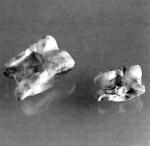
\includegraphics[width=6cm]{../grafici/astragals.jpeg}
\caption{ Astragalo. }
\label{fig:astragalo}
\end{center}
\end{figure}
Per simulare un astragalo su un computer
\begin{knitrout}
\definecolor{shadecolor}{rgb}{0.969, 0.969, 0.969}\color{fgcolor}\begin{kframe}
\begin{alltt}
\hlkwd{sample}\hlstd{(}\hlkwd{c}\hlstd{(}\hlnum{1}\hlstd{,}\hlnum{3}\hlstd{,}\hlnum{4}\hlstd{,}\hlnum{6}\hlstd{),}\hlnum{4}\hlstd{,}\hlkwc{replace}\hlstd{=T,}\hlkwc{prob}\hlstd{=}\hlkwd{c}\hlstd{(}\hlnum{0.1}\hlstd{,}\hlnum{0.4}\hlstd{,}\hlnum{0.4}\hlstd{,}\hlnum{0.1}\hlstd{))}
\end{alltt}
\begin{verbatim}
## [1] 3 3 3 3
\end{verbatim}
\end{kframe}
\end{knitrout}

Torniamo ora ai classici dadi a 6 facce.
Supponiamo di lanciare 100 volte un dado equo a 6 facce e di registrare in \texttt{x}
le uscite rilevate

\begin{knitrout}
\definecolor{shadecolor}{rgb}{0.969, 0.969, 0.969}\color{fgcolor}\begin{kframe}
\begin{alltt}
\hlkwd{set.seed}\hlstd{(}\hlnum{3}\hlstd{)}
\hlstd{dadi100}\hlkwb{<-}\hlkwd{sample}\hlstd{(}\hlnum{1}\hlopt{:}\hlnum{6}\hlstd{,}\hlnum{100}\hlstd{,}\hlkwc{replace}\hlstd{=T)}
\hlstd{dadi100}
\end{alltt}
\begin{verbatim}
##   [1] 2 5 3 2 4 4 1 2 4 4 4 4 4 4 6 5 1 5 6 2 2 1 1 1 2 5 4 6
##  [29] 4 5 3 3 2 3 2 3 6 2 4 2 2 5 2 4 3 2 1 1 2 5 2 2 6 6 6 6
##  [57] 3 2 1 2 5 1 5 1 5 2 5 4 3 1 5 5 6 6 4 4 1 1 5 5 5 4 3 1
##  [85] 6 6 2 3 4 6 1 2 3 5 6 2 2 2 2 5
\end{verbatim}
\end{kframe}
\end{knitrout}
Volendo invece simulare una combinazione da giocare al SuperEnalotto possiamo scrivere

\begin{knitrout}
\definecolor{shadecolor}{rgb}{0.969, 0.969, 0.969}\color{fgcolor}\begin{kframe}
\begin{alltt}
\hlstd{(x}\hlkwb{<-}\hlkwd{sample}\hlstd{(}\hlnum{1}\hlopt{:}\hlnum{90}\hlstd{,}\hlnum{6}\hlstd{,}\hlkwc{replace}\hlstd{=T))}
\end{alltt}
\begin{verbatim}
## [1] 69 62 19 65 55 31
\end{verbatim}
\end{kframe}
\end{knitrout}
I numeri usciti sono stati salvati  in una variabile \texttt{x}, per poter effettuare la ricerca di indicatori statistici.
Il comando che consente di ordinare una lista o un vettore \`e \texttt{sort}, esso pu\`o essere usato in associazione al nome di una variabile o di una lista, ossia:
\begin{equation}\texttt{sort}(\varia{variabile/lista})\end{equation}
Volendo ordinare i numeri precedentemente ricavati scriveremo
\begin{knitrout}
\definecolor{shadecolor}{rgb}{0.969, 0.969, 0.969}\color{fgcolor}\begin{kframe}
\begin{alltt}
\hlkwd{sort}\hlstd{(x)}
\end{alltt}
\begin{verbatim}
## [1] 19 31 55 62 65 69
\end{verbatim}
\end{kframe}
\end{knitrout}



\section{Statistica descrittiva: singola variabile}
\subsection{Indicatori statistici}
\begin{itemize}
\item{}Media.\vskip0pt
La media di una serie di numeri si ottiene con la funzione \texttt{mean} scrivendo:
$\texttt{mean}(\varia{variabile})$.
Ad esempio, lavorando con la lunghezza del sepalo di 150 piante di iris
\begin{knitrout}
\definecolor{shadecolor}{rgb}{0.969, 0.969, 0.969}\color{fgcolor}\begin{kframe}
\begin{alltt}
\hlstd{x}\hlkwb{=}\hlstd{iris[,}\hlnum{1}\hlstd{]}
\hlkwd{mean}\hlstd{(x)}
\end{alltt}
\begin{verbatim}
## [1] 5.843333
\end{verbatim}
\end{kframe}
\end{knitrout}
\item{}Varianza campionaria\vskip0pt
Si ottiene con la funzione predefinita di espressione:
\texttt{var}(\varia{variabile}).
Possiamo calcolare la varianza come
\begin{knitrout}
\definecolor{shadecolor}{rgb}{0.969, 0.969, 0.969}\color{fgcolor}\begin{kframe}
\begin{alltt}
\hlkwd{var}\hlstd{(x)}
\end{alltt}
\begin{verbatim}
## [1] 0.6856935
\end{verbatim}
\end{kframe}
\end{knitrout}
\item{}Deviazione Standard campionaria.\vskip0pt
Non \`e altro che la radice della varianza. Si ottiene con la funzione predefinita di espressione:
$\texttt{sd}(\varia{variabile})$.
Sempre basandosi sull'esempio precedente scriveremo
\begin{knitrout}
\definecolor{shadecolor}{rgb}{0.969, 0.969, 0.969}\color{fgcolor}\begin{kframe}
\begin{alltt}
\hlkwd{sd}\hlstd{(x)}
\end{alltt}
\begin{verbatim}
## [1] 0.8280661
\end{verbatim}
\end{kframe}
\end{knitrout}

\item{}Quantili. La notazione standard \`e semplicemente: \texttt{quantile}(\varia{variabile}) che determina i quartili e ci fornisce in uscita la statistica dei 5 numeri

\begin{knitrout}
\definecolor{shadecolor}{rgb}{0.969, 0.969, 0.969}\color{fgcolor}\begin{kframe}
\begin{alltt}
\hlkwd{quantile}\hlstd{(x)}
\end{alltt}
\begin{verbatim}
##   0%  25%  50%  75% 100% 
##  4.3  5.1  5.8  6.4  7.9
\end{verbatim}
\end{kframe}
\end{knitrout}
Volendo ricavare i decili dovremo scrivere:
$$\texttt{quantile}(\varia{variabile},\texttt{seq(0,1,by=0.1)})$$
in quanto vogliamo dividere l'intervallo $[0,1]$ a passo $0.1$

Nell'esempio:
\begin{knitrout}
\definecolor{shadecolor}{rgb}{0.969, 0.969, 0.969}\color{fgcolor}\begin{kframe}
\begin{alltt}
\hlkwd{quantile}\hlstd{(x,}\hlkwd{seq}\hlstd{(}\hlnum{0}\hlstd{,}\hlnum{1}\hlstd{,}\hlkwc{by}\hlstd{=}\hlnum{0.1}\hlstd{))}
\end{alltt}
\begin{verbatim}
##   0%  10%  20%  30%  40%  50%  60%  70%  80%  90% 100% 
## 4.30 4.80 5.00 5.27 5.60 5.80 6.10 6.30 6.52 6.90 7.90
\end{verbatim}
\end{kframe}
\end{knitrout}
Si noti che \texttt{quantile} ammette 9 varianti specificabili con l'opzione $\texttt{type}=n$ dove $n$ va da 1 a 9.
Per esempio
\begin{knitrout}
\definecolor{shadecolor}{rgb}{0.969, 0.969, 0.969}\color{fgcolor}\begin{kframe}
\begin{alltt}
\hlkwd{quantile}\hlstd{(x,}\hlkwc{type}\hlstd{=}\hlnum{2}\hlstd{)}
\end{alltt}
\begin{verbatim}
##   0%  25%  50%  75% 100% 
##  4.3  5.1  5.8  6.4  7.9
\end{verbatim}
\end{kframe}
\end{knitrout}
Sui dati in esame le 9 varianti coincidono. La convenzione da noi adottata corrisponde al numero 2
\end{itemize}
Per quanto riguarda gli indicatori statistici nel caso di dati ripetuti basta notare che se la lista $x$ contiene i valori e la lista $f$ le frequenze assolute il comando
$$\varia{rep}(x,f)$$ costruisce un'unica lista dei dati inclusiva delle ripetizioni.
Per esempio

\begin{knitrout}
\definecolor{shadecolor}{rgb}{0.969, 0.969, 0.969}\color{fgcolor}\begin{kframe}
\begin{alltt}
\hlstd{x}\hlkwb{=}\hlnum{1}\hlopt{:}\hlnum{6}
\hlstd{f}\hlkwb{=}\hlkwd{c}\hlstd{(}\hlnum{9}\hlstd{,}\hlnum{7}\hlstd{,}\hlnum{9}\hlstd{,}\hlnum{7}\hlstd{,}\hlnum{8}\hlstd{,}\hlnum{10}\hlstd{)}
\hlstd{(dati}\hlkwb{=}\hlkwd{rep}\hlstd{(x,f))}
\end{alltt}
\begin{verbatim}
##  [1] 1 1 1 1 1 1 1 1 1 2 2 2 2 2 2 2 3 3 3 3 3 3 3 3 3 4 4 4 4 4
## [31] 4 4 5 5 5 5 5 5 5 5 6 6 6 6 6 6 6 6 6 6
\end{verbatim}
\end{kframe}
\end{knitrout}
Ovviamente senza bisogno di visualizzare \texttt{dati} possiamo calcolarne tutti gli indicatori statistici.
Il comando
\begin{knitrout}
\definecolor{shadecolor}{rgb}{0.969, 0.969, 0.969}\color{fgcolor}\begin{kframe}
\begin{alltt}
\hlkwd{cumsum}\hlstd{(f)}
\end{alltt}
\begin{verbatim}
## [1]  9 16 25 32 40 50
\end{verbatim}
\end{kframe}
\end{knitrout}
restituisce le frequenze cumulate, dalle quali si possono ricavare facilmente la mediana
i quantili.

\subsection{Raggruppamenti in classi}


Consideriamo la rilevazione della temperatura media giornaliera di Milano nel mese di Gennaio 2016.
Scegliamo il mese
\begin{knitrout}
\definecolor{shadecolor}{rgb}{0.969, 0.969, 0.969}\color{fgcolor}\begin{kframe}
\begin{verbatim}
## > stringa="Milano/2016/Gennaio?format=csv"
\end{verbatim}
\end{kframe}
\end{knitrout}
\begin{knitrout}
\definecolor{shadecolor}{rgb}{0.969, 0.969, 0.969}\color{fgcolor}\begin{kframe}
\begin{alltt}
\hlstd{sito}\hlkwb{=}\hlstr{"http://www.ilmeteo.it/portale/archivio-meteo/"}
\hlstd{indirizzo}\hlkwb{=}\hlkwd{paste}\hlstd{(sito,stringa,}\hlkwc{sep}\hlstd{=}\hlstr{""}\hlstd{)}
\hlstd{meteo}\hlkwb{=}\hlkwd{read.table}\hlstd{(indirizzo,}\hlkwc{sep}\hlstd{=}\hlstr{";"}\hlstd{,}\hlkwc{header}\hlstd{=T)[,}\hlopt{-}\hlnum{1}\hlstd{]}
\end{alltt}
\end{kframe}
\end{knitrout}


\begin{knitrout}
\definecolor{shadecolor}{rgb}{0.969, 0.969, 0.969}\color{fgcolor}\begin{kframe}
\begin{alltt}
\hlkwd{options}\hlstd{(}\hlkwc{width} \hlstd{=} \hlnum{60}\hlstd{)}
\hlkwd{str}\hlstd{(meteo)}
\end{alltt}
\begin{verbatim}
## 'data.frame':	31 obs. of  15 variables:
##  $ LOCALITA         : Factor w/ 1 level "Milano": 1 1 1 1 1 1 1 1 1 1 ...
##  $ DATA             : Factor w/ 31 levels "1/1/2016","10/1/2016",..: 1 12 23 26 27 28 29 30 31 2 ...
##  $ TMEDIA..C        : int  1 1 1 2 3 5 3 2 5 5 ...
##  $ TMIN..C          : int  -2 0 0 1 2 3 -1 -1 3 4 ...
##  $ TMAX..C          : int  4 2 3 3 5 8 6 5 5 7 ...
##  $ PUNTORUGIADA..C  : int  1 1 1 1 2 2 2 2 4 5 ...
##  $ UMIDITA..        : int  97 97 96 93 89 85 88 89 95 95 ...
##  $ VISIBILITA.km    : int  2 2 3 4 5 5 8 7 2 3 ...
##  $ VENTOMEDIA.km.h  : int  6 5 7 7 6 8 5 7 6 5 ...
##  $ VENTOMAX.km.h    : int  11 9 11 11 11 13 11 17 11 11 ...
##  $ RAFFICA.km.h     : int  0 0 0 0 0 0 0 0 0 0 ...
##  $ PRESSIONESLM.mb  : int  1026 1019 1010 1000 1001 1001 1004 1009 1008 1004 ...
##  $ PRESSIONEMEDIA.mb: int  0 0 0 0 0 0 0 0 0 0 ...
##  $ PIOGGIA.mm       : int  0 0 0 0 0 0 0 0 0 0 ...
##  $ FENOMENI         : Factor w/ 7 levels "","nebbia ","neve nebbia ",..: 2 7 3 6 4 2 2 2 4 5 ...
\end{verbatim}
\end{kframe}
\end{knitrout}
A questo punto selezioniamo la colonna della temperatura media 
\begin{knitrout}
\definecolor{shadecolor}{rgb}{0.969, 0.969, 0.969}\color{fgcolor}\begin{kframe}
\begin{alltt}
\hlstd{meteo[,}\hlnum{3}\hlstd{]}\hlkwb{->}\hlstd{Milano;}
\hlstd{Milano}
\end{alltt}
\begin{verbatim}
##  [1]  1  1  1  2  3  5  3  2  5  5  6  5  7  2  5  5  6  0
## [19] -1  0  0  0  2  2  4  7  7  9 10  8  8
\end{verbatim}
\begin{alltt}
\hlkwd{quantile}\hlstd{(Milano)}
\end{alltt}
\begin{verbatim}
##   0%  25%  50%  75% 100% 
## -1.0  1.5  4.0  6.0 10.0
\end{verbatim}
\end{kframe}
\end{knitrout}
L'ultimo comando in particolare ci fornisce minimo e massimo dei dati.
Possiamo esaminare la serie temporale dei dati con i comandi
\begin{knitrout}
\definecolor{shadecolor}{rgb}{0.969, 0.969, 0.969}\color{fgcolor}\begin{kframe}
\begin{alltt}
\hlkwd{plot}\hlstd{(Milano,}\hlkwc{type}\hlstd{=}\hlstr{"l"}\hlstd{,}\hlkwc{xlab}\hlstd{=}\hlkwd{paste}\hlstd{(m,anno,} \hlstr{"a milano"}\hlstd{),}\hlkwc{ylab}\hlstd{=}\hlstr{"temperatura media"}\hlstd{)}
\end{alltt}


{\ttfamily\noindent\bfseries\color{errorcolor}{\#\# Error in getMetricsFromLatex(TeXMetrics, verbose = verbose): \\\#\# TeX was unable to calculate metrics for the following string\\\#\# or character:\\\#\# \\\#\# 	m\\\#\# \\\#\# Common reasons for failure include:\\\#\#\ \  * The string contains a character which is special to LaTeX unless\\\#\#\ \ \ \  escaped properly, such as \% or \$.\\\#\#\ \  * The string makes use of LaTeX commands provided by a package and\\\#\#\ \ \ \  the tikzDevice was not told to load the package.\\\#\# \\\#\# The contents of the LaTeX log of the aborted run have been printed above,\\\#\# it may contain additional details as to why the metric calculation failed.}}\end{kframe}
\end{knitrout}
ottenendo la figura~\ref{fig:datiist}
\begin{figure}[htbp]
\begin{center}
\begin{knitrout}
\definecolor{shadecolor}{rgb}{0.969, 0.969, 0.969}\color{fgcolor}\begin{kframe}


{\ttfamily\noindent\bfseries\color{errorcolor}{\#\# Error in getMetricsFromLatex(TeXMetrics, verbose = verbose): \\\#\# TeX was unable to calculate metrics for the following string\\\#\# or character:\\\#\# \\\#\# 	m\\\#\# \\\#\# Common reasons for failure include:\\\#\#\ \  * The string contains a character which is special to LaTeX unless\\\#\#\ \ \ \  escaped properly, such as \% or \$.\\\#\#\ \  * The string makes use of LaTeX commands provided by a package and\\\#\#\ \ \ \  the tikzDevice was not told to load the package.\\\#\# \\\#\# The contents of the LaTeX log of the aborted run have been printed above,\\\#\# it may contain additional details as to why the metric calculation failed.}}\end{kframe}

{\centering 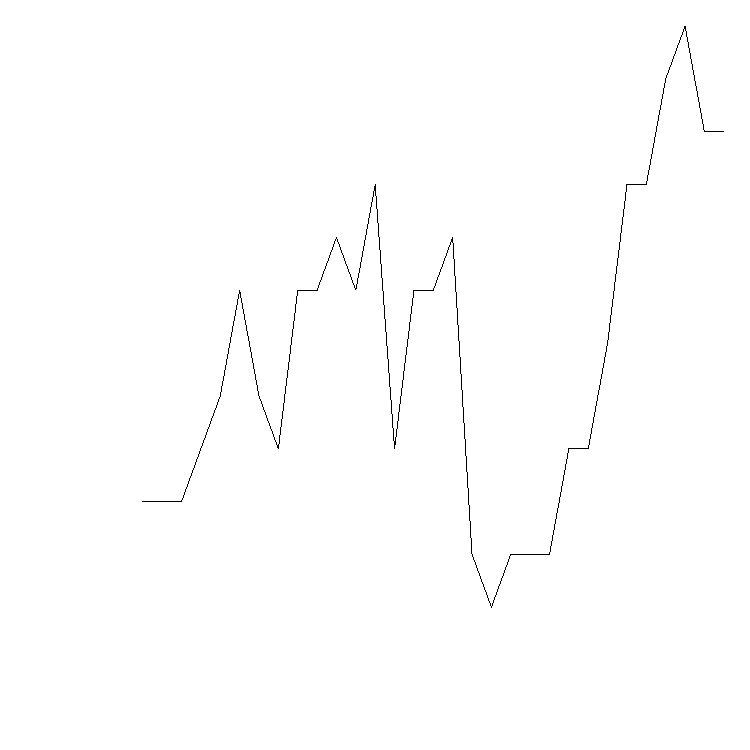
\includegraphics[width=\maxwidth]{figure/graphics-unnamed-chunk-98-1} 

}



\end{knitrout}
\caption{ Andamento della temperatura a Gennaio 2016  a Milano. }
\label{fig:datiist}
\end{center}
\end{figure}

Raggruppiamo ora i dati in classi comprese  tra due estremi che comprendano certamente tutti i dati, per esempio \ensuremath{-2} e 10, decidendo di applicare un passo di 2 e vedere come si distribuiscono. Il comando \texttt{cut} associa a ciascun dato la classe di appartenenza selezionata in base ai punti di taglio.

\begin{knitrout}
\definecolor{shadecolor}{rgb}{0.969, 0.969, 0.969}\color{fgcolor}\begin{kframe}
\begin{alltt}
\hlstd{tagli}\hlkwb{=}\hlkwd{c}\hlstd{(}\hlopt{-}\hlnum{2}\hlstd{,}\hlnum{0}\hlstd{,}\hlnum{2}\hlstd{,}\hlnum{4}\hlstd{,}\hlnum{6}\hlstd{,}\hlnum{10}\hlstd{)}
\hlkwd{cut}\hlstd{(Milano,}\hlkwc{breaks}\hlstd{=tagli)}
\end{alltt}
\begin{verbatim}
##  [1] (0,2]  (0,2]  (0,2]  (0,2]  (2,4]  (4,6]  (2,4]  (0,2] 
##  [9] (4,6]  (4,6]  (4,6]  (4,6]  (6,10] (0,2]  (4,6]  (4,6] 
## [17] (4,6]  (-2,0] (-2,0] (-2,0] (-2,0] (-2,0] (0,2]  (0,2] 
## [25] (2,4]  (6,10] (6,10] (6,10] (6,10] (6,10] (6,10]
## Levels: (-2,0] (0,2] (2,4] (4,6] (6,10]
\end{verbatim}
\end{kframe}
\end{knitrout}

Il comando \texttt{table} conta i dati di ciascuna classe

\begin{knitrout}
\definecolor{shadecolor}{rgb}{0.969, 0.969, 0.969}\color{fgcolor}\begin{kframe}
\begin{alltt}
\hlkwd{table}\hlstd{(}\hlkwd{cut}\hlstd{(Milano,}\hlkwc{breaks}\hlstd{=tagli))}
\end{alltt}
\begin{verbatim}
## 
## (-2,0]  (0,2]  (2,4]  (4,6] (6,10] 
##      5      8      3      8      7
\end{verbatim}
\end{kframe}
\end{knitrout}
Si noti che la suddivisione in classi prevede intervalli aperti a sinistra e chiusi a destra.
Per suddividere in modo che gli intervalli siano chiusi a sinistra e aperti a destra si specifica il parametro \texttt{right=FALSE}.
Possiamo anche usare il comando \texttt{seq} per specificare i tagli.
 \begin{eqnarray*}
\texttt{table(cut}( \varia{variabile},\texttt{breaks=seq}(\varia{estremo inf},\\
\varia{estremo sup},\texttt{by}=\varia{passo}),\texttt{right=TRUE}))
\end{eqnarray*}
o in modo  pi\`u generale
\begin{eqnarray*}
&\texttt{table(cut}(\varia{ variabile},\\
&\texttt{breaks=c}(\varia{estremo\; inferiore}, \ldots,\varia{estremo superiore}))
\end{eqnarray*}
estremamente utile in quanto consente di raggruppare i dati in classi non necessariamente di ugual ampiezza.
\begin{knitrout}
\definecolor{shadecolor}{rgb}{0.969, 0.969, 0.969}\color{fgcolor}\begin{kframe}
\begin{alltt}
\hlkwd{table}\hlstd{(}\hlkwd{cut}\hlstd{(Milano,}\hlkwc{breaks}\hlstd{=}\hlkwd{c}\hlstd{(}\hlopt{-}\hlnum{3}\hlstd{,}\hlnum{1}\hlstd{,}\hlnum{3}\hlstd{,}\hlnum{4}\hlstd{,}\hlnum{5}\hlstd{,}\hlnum{6}\hlstd{,}\hlnum{8}\hlstd{,}\hlnum{10}\hlstd{)))}
\end{alltt}
\begin{verbatim}
## 
## (-3,1]  (1,3]  (3,4]  (4,5]  (5,6]  (6,8] (8,10] 
##      8      7      1      6      2      5      2
\end{verbatim}
\end{kframe}
\end{knitrout}
Volendo raggruppare in classi i dati delle precedenti uscite del dado possiamo scrivere
\begin{knitrout}
\definecolor{shadecolor}{rgb}{0.969, 0.969, 0.969}\color{fgcolor}\begin{kframe}
\begin{alltt}
\hlkwd{table}\hlstd{(}\hlkwd{cut}\hlstd{(dadi100,}\hlkwc{breaks}\hlstd{=}\hlnum{0}\hlopt{:}\hlnum{6}\hlstd{))}
\end{alltt}
\begin{verbatim}
## 
## (0,1] (1,2] (2,3] (3,4] (4,5] (5,6] 
##    15    25    11    17    18    14
\end{verbatim}
\end{kframe}
\end{knitrout}
Se scegliamo di chiudere a sinistra gli intervalli dobbiamo però includere il 7 altrimenti 
il valore 6 non risutlerebbe incluso.
\begin{knitrout}
\definecolor{shadecolor}{rgb}{0.969, 0.969, 0.969}\color{fgcolor}\begin{kframe}
\begin{alltt}
\hlkwd{table}\hlstd{(}\hlkwd{cut}\hlstd{(dadi100,}\hlkwc{breaks}\hlstd{=} \hlnum{1}\hlopt{:}\hlnum{7}\hlstd{,}\hlkwc{right}\hlstd{=}\hlnum{FALSE}\hlstd{))}
\end{alltt}
\begin{verbatim}
## 
## [1,2) [2,3) [3,4) [4,5) [5,6) [6,7) 
##    15    25    11    17    18    14
\end{verbatim}
\end{kframe}
\end{knitrout}

\subsection{Areogrammi}
Il comando generico per generare un istogramma \`e:
\begin{equation*}
\texttt{hist}(\varia{variabile})\index{\texttt{hist}}
\end{equation*}
che segue per\`o la struttura del comando \texttt{cut}. L'ampiezza di ciascuna classe salvo diversamente indicato \`e costante e decisa da \textsf{R}.
\`E  possibile variare tale condizione definendo una lista con i punti di taglio ({\it cutoff}) delle classi volute:
\begin{equation} \texttt{hist}(\varia{variabile},\texttt{c}(\varia{valore}_1, \varia{valore}_2, \ldots))
\end{equation}
Per esempio se \texttt{dadi100} rappresenta le solite 100 uscite del lancio del dado, il comando
\begin{knitrout}
\definecolor{shadecolor}{rgb}{0.969, 0.969, 0.969}\color{fgcolor}\begin{kframe}
\begin{alltt}
\hlkwd{par}\hlstd{(}\hlkwc{mfrow}\hlstd{=}\hlkwd{c}\hlstd{(}\hlnum{1}\hlstd{,}\hlnum{2}\hlstd{))}
\hlkwd{hist}\hlstd{(dadi100,}\hlkwc{breaks}\hlstd{=}\hlkwd{seq}\hlstd{(}\hlnum{0.5}\hlstd{,}\hlnum{6.5}\hlstd{,}\hlnum{1}\hlstd{),}\hlkwc{col}\hlstd{=}\hlstr{"red"}\hlstd{)}
\end{alltt}


{\ttfamily\noindent\bfseries\color{errorcolor}{\#\# Error in getMetricsFromLatex(TeXMetrics, verbose = verbose): \\\#\# TeX was unable to calculate metrics for the following string\\\#\# or character:\\\#\# \\\#\# 	Histogram of dadi100\\\#\# \\\#\# Common reasons for failure include:\\\#\#\ \  * The string contains a character which is special to LaTeX unless\\\#\#\ \ \ \  escaped properly, such as \% or \$.\\\#\#\ \  * The string makes use of LaTeX commands provided by a package and\\\#\#\ \ \ \  the tikzDevice was not told to load the package.\\\#\# \\\#\# The contents of the LaTeX log of the aborted run have been printed above,\\\#\# it may contain additional details as to why the metric calculation failed.}}\begin{alltt}
\hlkwd{hist}\hlstd{(dadi100,}\hlkwc{freq}\hlstd{=}\hlnum{FALSE}\hlstd{,}\hlkwc{breaks}\hlstd{=}\hlkwd{seq}\hlstd{(}\hlnum{0.5}\hlstd{,}\hlnum{6.5}\hlstd{,}\hlnum{1}\hlstd{),}\hlkwc{col}\hlstd{=}\hlstr{"blue"}\hlstd{)}
\end{alltt}


{\ttfamily\noindent\bfseries\color{errorcolor}{\#\# Error in getMetricsFromLatex(TeXMetrics, verbose = verbose): \\\#\# TeX was unable to calculate metrics for the following string\\\#\# or character:\\\#\# \\\#\# 	Histogram of dadi100\\\#\# \\\#\# Common reasons for failure include:\\\#\#\ \  * The string contains a character which is special to LaTeX unless\\\#\#\ \ \ \  escaped properly, such as \% or \$.\\\#\#\ \  * The string makes use of LaTeX commands provided by a package and\\\#\#\ \ \ \  the tikzDevice was not told to load the package.\\\#\# \\\#\# The contents of the LaTeX log of the aborted run have been printed above,\\\#\# it may contain additional details as to why the metric calculation failed.}}\end{kframe}
\end{knitrout}
\begin{figure}[htbp]
\begin{center}
\begin{knitrout}
\definecolor{shadecolor}{rgb}{0.969, 0.969, 0.969}\color{fgcolor}\begin{kframe}


{\ttfamily\noindent\bfseries\color{errorcolor}{\#\# Error in getMetricsFromLatex(TeXMetrics, verbose = verbose): \\\#\# TeX was unable to calculate metrics for the following string\\\#\# or character:\\\#\# \\\#\# 	Histogram of dadi100\\\#\# \\\#\# Common reasons for failure include:\\\#\#\ \  * The string contains a character which is special to LaTeX unless\\\#\#\ \ \ \  escaped properly, such as \% or \$.\\\#\#\ \  * The string makes use of LaTeX commands provided by a package and\\\#\#\ \ \ \  the tikzDevice was not told to load the package.\\\#\# \\\#\# The contents of the LaTeX log of the aborted run have been printed above,\\\#\# it may contain additional details as to why the metric calculation failed.}}

{\ttfamily\noindent\bfseries\color{errorcolor}{\#\# Error in getMetricsFromLatex(TeXMetrics, verbose = verbose): \\\#\# TeX was unable to calculate metrics for the following string\\\#\# or character:\\\#\# \\\#\# 	Histogram of dadi100\\\#\# \\\#\# Common reasons for failure include:\\\#\#\ \  * The string contains a character which is special to LaTeX unless\\\#\#\ \ \ \  escaped properly, such as \% or \$.\\\#\#\ \  * The string makes use of LaTeX commands provided by a package and\\\#\#\ \ \ \  the tikzDevice was not told to load the package.\\\#\# \\\#\# The contents of the LaTeX log of the aborted run have been printed above,\\\#\# it may contain additional details as to why the metric calculation failed.}}\end{kframe}

{\centering 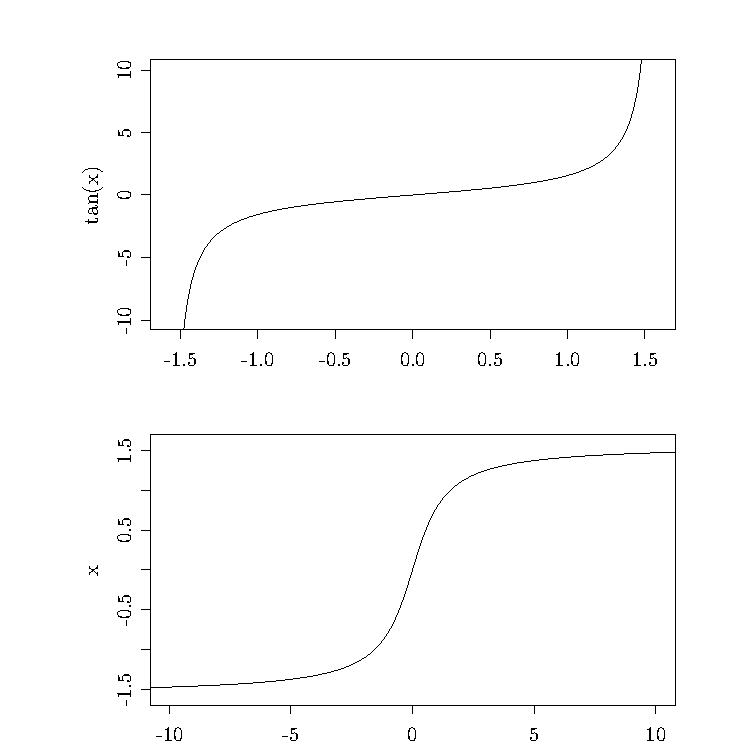
\includegraphics[width=\maxwidth]{figure/graphics-unnamed-chunk-105-1} 

}



\end{knitrout}
\caption{Diagramma a colonne e areogramma per il lancio di un dado.}
\label{fig:datidado}
\end{center}
\end{figure}
genera l'istogramma (in rosso, a sinistra Figura~\ref{fig:datiist}) con le frequenze assolute delle classi in ordinata. La sequenza dei punti di taglio \`e stata scelta in modo che i numeri interi da 1 a 6 siano al centro delle classi corrispondenti. Se invece volessimo creare un areogramma  (ossia avere un tracciato per cui le aree siano pari alle frequenze relative) a partire dalle stesse uscite dovremo imporre il parametro \texttt{freq=FALSE} otterremo il pannello a destra (in blu) della figura~(\ref{fig:datiist}). Avendo scelto classi di ampiezza costante i 2 grafici differiscono semplicemente per un cambio di scala sull'asse $y$.

In modo simile possiamo tracciare un areogramma  dei dati nella variabile \texttt{milano}
\begin{knitrout}
\definecolor{shadecolor}{rgb}{0.969, 0.969, 0.969}\color{fgcolor}\begin{kframe}
\begin{alltt}
\hlkwd{par}\hlstd{(}\hlkwc{mfrow}\hlstd{=}\hlkwd{c}\hlstd{(}\hlnum{1}\hlstd{,}\hlnum{2}\hlstd{))}
\hlkwd{hist}\hlstd{(Milano,} \hlkwc{col}\hlstd{=}\hlstr{"green"}\hlstd{,}\hlkwc{freq}\hlstd{=}\hlnum{FALSE}\hlstd{,}\hlkwc{right}\hlstd{=}\hlnum{FALSE}\hlstd{,}
\hlkwc{main}\hlstd{=}\hlstr{"Cutoff automatici"}\hlstd{)}
\end{alltt}
\end{kframe}
\end{knitrout}
lasciando \textsf{R} libero di scegliere i punti di taglio (pannelli a sinistra della figura \ref{fig:datiistmilano}) o scegliendoli a nostra volta (pannelli a destra della stessa figura  \ref{fig:datiistmilano})

\begin{knitrout}
\definecolor{shadecolor}{rgb}{0.969, 0.969, 0.969}\color{fgcolor}\begin{kframe}
\begin{alltt}
\hlkwd{hist}\hlstd{(Milano,}\hlkwc{col}\hlstd{=}\hlstr{"red"}\hlstd{,}\hlkwc{freq}\hlstd{=}\hlnum{FALSE}\hlstd{,}
\hlkwc{breaks}\hlstd{=}\hlkwd{unique}\hlstd{(}\hlkwd{as.vector}\hlstd{(}\hlkwd{quantile}\hlstd{(Milano,}\hlkwd{seq}\hlstd{(}\hlnum{0}\hlstd{,}\hlnum{1}\hlstd{,}\hlkwc{by}\hlstd{=}\hlnum{1}\hlopt{/}\hlnum{6}\hlstd{)))),}
\hlkwc{main}\hlstd{=}\hlstr{"Cutoff personalizzati"}\hlstd{)}
\end{alltt}


{\ttfamily\noindent\bfseries\color{errorcolor}{\#\# Error in getMetricsFromLatex(TeXMetrics, verbose = verbose): \\\#\# TeX was unable to calculate metrics for the following string\\\#\# or character:\\\#\# \\\#\# 	Cutoff personalizzati\\\#\# \\\#\# Common reasons for failure include:\\\#\#\ \  * The string contains a character which is special to LaTeX unless\\\#\#\ \ \ \  escaped properly, such as \% or \$.\\\#\#\ \  * The string makes use of LaTeX commands provided by a package and\\\#\#\ \ \ \  the tikzDevice was not told to load the package.\\\#\# \\\#\# The contents of the LaTeX log of the aborted run have been printed above,\\\#\# it may contain additional details as to why the metric calculation failed.}}\end{kframe}

{\centering 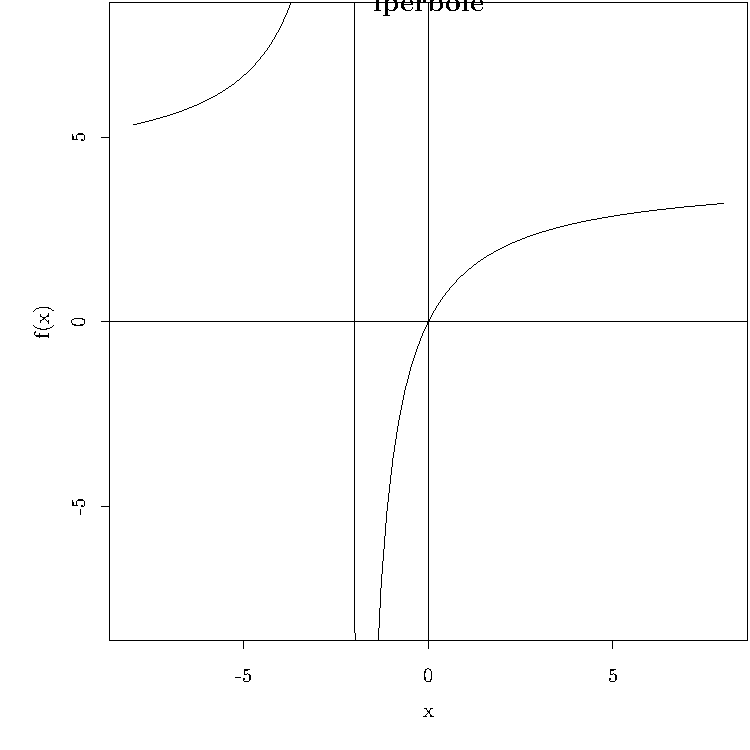
\includegraphics[width=\maxwidth]{figure/graphics-unnamed-chunk-108-1} 

}



\end{knitrout}
\begin{figure}[htbp]
\begin{center}
\begin{knitrout}
\definecolor{shadecolor}{rgb}{0.969, 0.969, 0.969}\color{fgcolor}\begin{kframe}


{\ttfamily\noindent\bfseries\color{errorcolor}{\#\# Error in getMetricsFromLatex(TeXMetrics, verbose = verbose): \\\#\# TeX was unable to calculate metrics for the following string\\\#\# or character:\\\#\# \\\#\# 	Cutoff automatici\\\#\# \\\#\# Common reasons for failure include:\\\#\#\ \  * The string contains a character which is special to LaTeX unless\\\#\#\ \ \ \  escaped properly, such as \% or \$.\\\#\#\ \  * The string makes use of LaTeX commands provided by a package and\\\#\#\ \ \ \  the tikzDevice was not told to load the package.\\\#\# \\\#\# The contents of the LaTeX log of the aborted run have been printed above,\\\#\# it may contain additional details as to why the metric calculation failed.}}

{\ttfamily\noindent\bfseries\color{errorcolor}{\#\# Error in getMetricsFromLatex(TeXMetrics, verbose = verbose): \\\#\# TeX was unable to calculate metrics for the following string\\\#\# or character:\\\#\# \\\#\# 	Cutoff personalizzati\\\#\# \\\#\# Common reasons for failure include:\\\#\#\ \  * The string contains a character which is special to LaTeX unless\\\#\#\ \ \ \  escaped properly, such as \% or \$.\\\#\#\ \  * The string makes use of LaTeX commands provided by a package and\\\#\#\ \ \ \  the tikzDevice was not told to load the package.\\\#\# \\\#\# The contents of the LaTeX log of the aborted run have been printed above,\\\#\# it may contain additional details as to why the metric calculation failed.}}\end{kframe}

{\centering 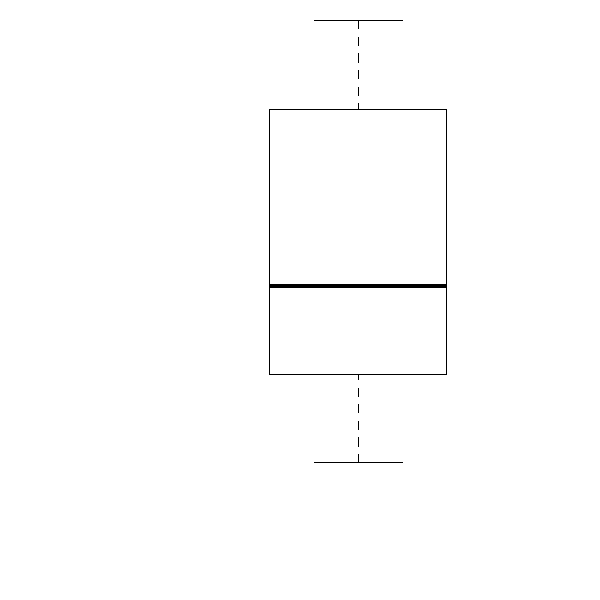
\includegraphics[width=\maxwidth]{figure/graphics-unnamed-chunk-109-1} 

}



\end{knitrout}
\caption{ Areogramma dei dati della temperatura. Scelta automatica dei punti di taglio.}
\label{fig:datiistmilano}
\end{center}
\end{figure}
Si noti la stabilit\`a degli areogrammi rispetto ai cambi nella suddivisione.
\subsection{Generazione di boxplot}

Il \texttt{boxplot}  \`e una rappresentazione grafica immediata della statistica dei 5 numeri e simultaneamente ci  segnala eventuali punti discordanti o anomali, {\it outlier}.
Il comando generico \`e: \begin{equation}\texttt{boxplot}(\varia{variabile})\end{equation}
prendendo il vettore $x$ contenente i risultati di 100 lanci
otteniamo la figura~\ref{fig:boxplotdado}
\begin{figure}[htbp]
\begin{center}
\begin{knitrout}
\definecolor{shadecolor}{rgb}{0.969, 0.969, 0.969}\color{fgcolor}\begin{kframe}
\begin{alltt}
\hlkwd{boxplot}\hlstd{(dadi100)}
\end{alltt}


{\ttfamily\noindent\bfseries\color{errorcolor}{\#\# Error in getMetricsFromLatex(TeXMetrics, verbose = verbose): \\\#\# TeX was unable to calculate metrics for the following string\\\#\# or character:\\\#\# \\\#\# 	m\\\#\# \\\#\# Common reasons for failure include:\\\#\#\ \  * The string contains a character which is special to LaTeX unless\\\#\#\ \ \ \  escaped properly, such as \% or \$.\\\#\#\ \  * The string makes use of LaTeX commands provided by a package and\\\#\#\ \ \ \  the tikzDevice was not told to load the package.\\\#\# \\\#\# The contents of the LaTeX log of the aborted run have been printed above,\\\#\# it may contain additional details as to why the metric calculation failed.}}\end{kframe}

{\centering 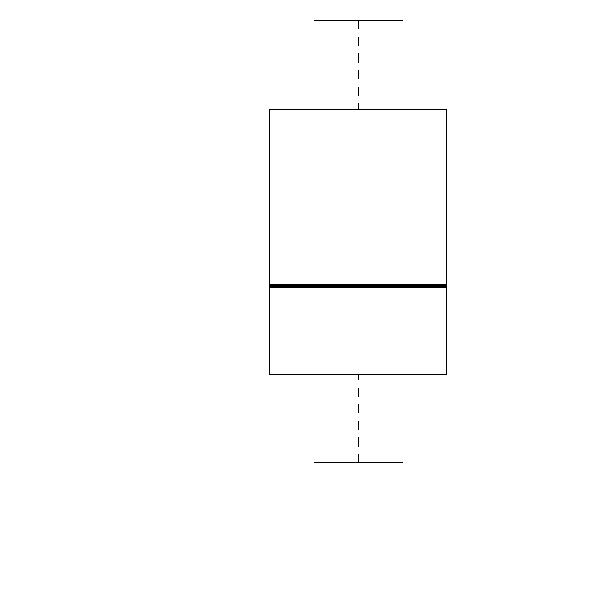
\includegraphics[width=\maxwidth]{figure/graphics-unnamed-chunk-110-1} 

}



\end{knitrout}
\caption{Boxplot dei risultati del lancio di un dado}
\label{fig:boxplotdado}
\end{center}
\end{figure}
da cui si evince che il valore massimo dei dati \`e 6, il minimo \`e 1 e non ci sono punti anomali, per cui non vi sono dati anomali, altrimenti evidenziati da un pallino. Si legge inoltre il valore di mediana (4) primo quartile (2) e terzo quartile (5).

\subsection{Creazione di grafici a torta}

Il comando \texttt{pie} consente, partendo da una tabella, di tracciare il diagramma a torta per una variabile nominale raggruppata in classi. Il comando \`e

\begin{equation*}\texttt{pie(table}(\varia{variabile} ))
\end{equation*}
ad esempio (facendo riferimento ai precedenti dati):
\begin{knitrout}
\definecolor{shadecolor}{rgb}{0.969, 0.969, 0.969}\color{fgcolor}\begin{kframe}
\begin{alltt}
\hlkwd{pie}\hlstd{(}\hlkwd{table}\hlstd{(dadi100))}
\end{alltt}


{\ttfamily\noindent\bfseries\color{errorcolor}{\#\# Error in getMetricsFromLatex(TeXMetrics, verbose = verbose): \\\#\# TeX was unable to calculate metrics for the following string\\\#\# or character:\\\#\# \\\#\# 	1\\\#\# \\\#\# Common reasons for failure include:\\\#\#\ \  * The string contains a character which is special to LaTeX unless\\\#\#\ \ \ \  escaped properly, such as \% or \$.\\\#\#\ \  * The string makes use of LaTeX commands provided by a package and\\\#\#\ \ \ \  the tikzDevice was not told to load the package.\\\#\# \\\#\# The contents of the LaTeX log of the aborted run have been printed above,\\\#\# it may contain additional details as to why the metric calculation failed.}}\end{kframe}
\end{knitrout}
fornisce in uscita  la Figura~\ref{fig:pie}
\begin{figure}[htbp]
\begin{center}
\begin{knitrout}
\definecolor{shadecolor}{rgb}{0.969, 0.969, 0.969}\color{fgcolor}\begin{kframe}


{\ttfamily\noindent\bfseries\color{errorcolor}{\#\# Error in getMetricsFromLatex(TeXMetrics, verbose = verbose): \\\#\# TeX was unable to calculate metrics for the following string\\\#\# or character:\\\#\# \\\#\# 	1\\\#\# \\\#\# Common reasons for failure include:\\\#\#\ \  * The string contains a character which is special to LaTeX unless\\\#\#\ \ \ \  escaped properly, such as \% or \$.\\\#\#\ \  * The string makes use of LaTeX commands provided by a package and\\\#\#\ \ \ \  the tikzDevice was not told to load the package.\\\#\# \\\#\# The contents of the LaTeX log of the aborted run have been printed above,\\\#\# it may contain additional details as to why the metric calculation failed.}}\end{kframe}

{\centering 
\includegraphics[width=\maxwidth]{figure/graphics-unnamed-chunk-112-1} 

}



\end{knitrout}
\caption{Diagramma a torta per il lancio di un dado equo.}
\label{fig:pie}
\end{center}
\end{figure}
\begin{shaded}{Costruire una matrice contenente le coordinate di 50 punti nel rettangolo $[0,4]\times [0,2]$ in due dimensioni (generate utilizzando il generatore di numeri pseudocasuali). Produrre un grafico con due pannelli, dove il primo pannello \`e uno scatter-plot}
\end{shaded}
\section{Variabili doppie e rette di regressione}
Supponiamo di misurare la concentrazione di acido lattico muscolare durante uno sforzo di 10 minuti,
\begin{knitrout}
\definecolor{shadecolor}{rgb}{0.969, 0.969, 0.969}\color{fgcolor}\begin{kframe}
\begin{alltt}
\hlstd{x}\hlkwb{<-}\hlstd{tempo}\hlkwb{<-}\hlkwd{c}\hlstd{(}\hlnum{1}\hlstd{,}\hlnum{2}\hlstd{,}\hlnum{3}\hlstd{,}\hlnum{4}\hlstd{,}\hlnum{5}\hlstd{,}\hlnum{6}\hlstd{,}\hlnum{7}\hlstd{,}\hlnum{8}\hlstd{,}\hlnum{9}\hlstd{,}\hlnum{10}\hlstd{)}
\hlstd{y}\hlkwb{<-}\hlstd{concentrazione}\hlkwb{<-}\hlkwd{c}\hlstd{(}\hlnum{0.3}\hlstd{,}\hlnum{0.65}\hlstd{,}\hlnum{0.7}\hlstd{,}\hlnum{0.8}\hlstd{,}\hlnum{0.95}\hlstd{,}\hlnum{1.05}\hlstd{,}\hlnum{1.3}\hlstd{,}\hlnum{1.7}\hlstd{,}\hlnum{1.9}\hlstd{,}
\hlnum{2.5}\hlstd{)}
\end{alltt}
\end{kframe}
\end{knitrout}
Per analizzare questi dati conviene preliminarmente tracciarne un diagramma a dispersione.
\begin{figure}[htbp]
\begin{center}
\begin{knitrout}
\definecolor{shadecolor}{rgb}{0.969, 0.969, 0.969}\color{fgcolor}\begin{kframe}
\begin{alltt}
\hlkwd{plot}\hlstd{(x,y)}
\end{alltt}


{\ttfamily\noindent\bfseries\color{errorcolor}{\#\# Error in getMetricsFromLatex(TeXMetrics, verbose = verbose): \\\#\# TeX was unable to calculate metrics for the following string\\\#\# or character:\\\#\# \\\#\# 	m\\\#\# \\\#\# Common reasons for failure include:\\\#\#\ \  * The string contains a character which is special to LaTeX unless\\\#\#\ \ \ \  escaped properly, such as \% or \$.\\\#\#\ \  * The string makes use of LaTeX commands provided by a package and\\\#\#\ \ \ \  the tikzDevice was not told to load the package.\\\#\# \\\#\# The contents of the LaTeX log of the aborted run have been printed above,\\\#\# it may contain additional details as to why the metric calculation failed.}}\end{kframe}

{\centering 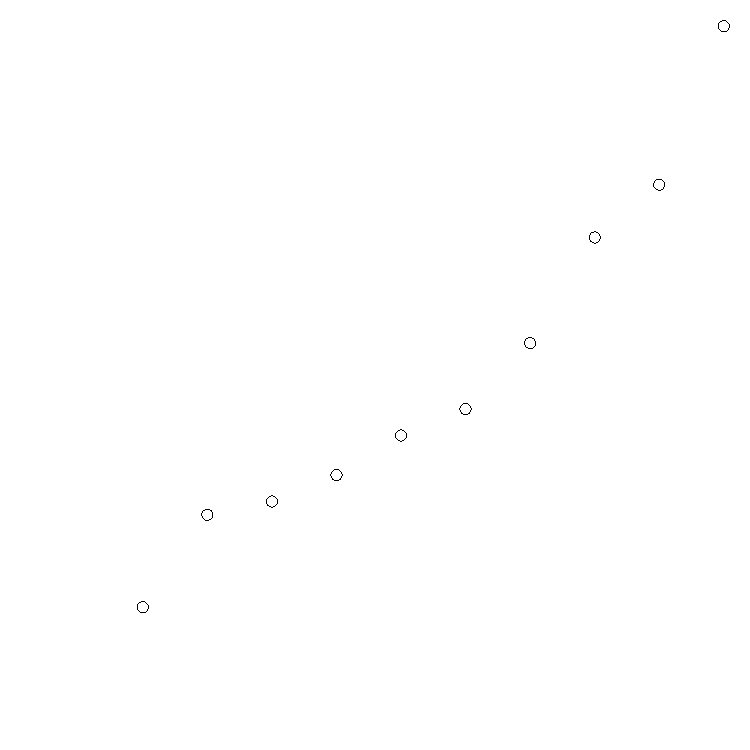
\includegraphics[width=\maxwidth]{figure/graphics-unnamed-chunk-114-1} 

}



\end{knitrout}
\caption{Diagramma a dispersione tempo/concentrazione.}
\label{fig:scatte}
\end{center}
\end{figure}
Possiamo inoltre determinare il coefficiente di correlazione lineare
\begin{knitrout}
\definecolor{shadecolor}{rgb}{0.969, 0.969, 0.969}\color{fgcolor}\begin{kframe}
\begin{alltt}
\hlkwd{cor}\hlstd{(x,y)}
\end{alltt}
\begin{verbatim}
## [1] 0.9620456
\end{verbatim}
\end{kframe}
\end{knitrout}
Per definire un modello di relazione lineare occorre usare il comando \texttt{lm} (\varia{linear model}).
Nella sua generica forma il comando \`e espresso come\footnote{ Per digitare la tilde  \mytilde\;  su Mac premere ALT 5 su PC invece il tasto Alt Gr (attivazione del codice ASCII) e sul tastierino numerico digitare il numero 126. Lavorando su un portatile il tastierino numerico \`e spesso incorporato nella tastiera con colorazione blu dei tasti.}
$$\texttt{lm}(\varia{y} \sim  \varia{x})$$
Otteniamo i valori di pendenza e intercetta.

Possiamo tracciare la retta di regressione con il comando \texttt{abline}.
\begin{knitrout}
\definecolor{shadecolor}{rgb}{0.969, 0.969, 0.969}\color{fgcolor}\begin{kframe}
\begin{alltt}
\hlkwd{plot}\hlstd{(x,y,}\hlkwc{pch}\hlstd{=}\hlnum{19}\hlstd{,}\hlkwc{col}\hlstd{=}\hlstr{"red"}\hlstd{)}
\end{alltt}


{\ttfamily\noindent\bfseries\color{errorcolor}{\#\# Error in getMetricsFromLatex(TeXMetrics, verbose = verbose): \\\#\# TeX was unable to calculate metrics for the following string\\\#\# or character:\\\#\# \\\#\# 	m\\\#\# \\\#\# Common reasons for failure include:\\\#\#\ \  * The string contains a character which is special to LaTeX unless\\\#\#\ \ \ \  escaped properly, such as \% or \$.\\\#\#\ \  * The string makes use of LaTeX commands provided by a package and\\\#\#\ \ \ \  the tikzDevice was not told to load the package.\\\#\# \\\#\# The contents of the LaTeX log of the aborted run have been printed above,\\\#\# it may contain additional details as to why the metric calculation failed.}}\begin{alltt}
\hlkwd{abline}\hlstd{(}\hlkwd{lm}\hlstd{(y}\hlopt{~}\hlstd{x),}\hlkwc{col}\hlstd{=}\hlstr{"blue"}\hlstd{)}
\end{alltt}
\end{kframe}
\end{knitrout}
Per determinare  la retta di regressione sulle $y$ dobbiamo invertire $x$ e $y$.
\begin{knitrout}
\definecolor{shadecolor}{rgb}{0.969, 0.969, 0.969}\color{fgcolor}\begin{kframe}
\begin{alltt}
\hlstd{(modellox}\hlkwb{=}\hlkwd{lm}\hlstd{(x}\hlopt{~}\hlstd{y))}
\end{alltt}
\begin{verbatim}
## 
## Call:
## lm(formula = x ~ y)
## 
## Coefficients:
## (Intercept)            y  
##      0.3516       4.3446
\end{verbatim}
\begin{alltt}
\hlstd{coeff}\hlkwb{=}\hlstd{modellox}\hlopt{$}\hlstd{coefficients}
\hlstd{(a}\hlkwb{=}\hlnum{1}\hlopt{/}\hlstd{coeff[}\hlnum{2}\hlstd{])}
\end{alltt}
\begin{verbatim}
##         y 
## 0.2301707
\end{verbatim}
\begin{alltt}
\hlstd{(b}\hlkwb{=}\hlopt{-}\hlstd{coeff[}\hlnum{1}\hlstd{]}\hlopt{/}\hlstd{coeff[}\hlnum{2}\hlstd{])}
\end{alltt}
\begin{verbatim}
## (Intercept) 
## -0.08093883
\end{verbatim}
\begin{alltt}
\hlkwd{abline}\hlstd{(b,a,}\hlkwc{col}\hlstd{=}\hlstr{"green"}\hlstd{)}
\end{alltt}


{\ttfamily\noindent\bfseries\color{errorcolor}{\#\# Error in int\_abline(a = a, b = b, h = h, v = v, untf = untf, ...): plot.new has not been called yet}}\end{kframe}
\end{knitrout}
In tal modo otteniamo il grafico~\ref{fig:duerettex}.
\begin{center}
\begin{figure}[htbp]
\begin{knitrout}
\definecolor{shadecolor}{rgb}{0.969, 0.969, 0.969}\color{fgcolor}\begin{kframe}


{\ttfamily\noindent\bfseries\color{errorcolor}{\#\# Error in getMetricsFromLatex(TeXMetrics, verbose = verbose): \\\#\# TeX was unable to calculate metrics for the following string\\\#\# or character:\\\#\# \\\#\# 	m\\\#\# \\\#\# Common reasons for failure include:\\\#\#\ \  * The string contains a character which is special to LaTeX unless\\\#\#\ \ \ \  escaped properly, such as \% or \$.\\\#\#\ \  * The string makes use of LaTeX commands provided by a package and\\\#\#\ \ \ \  the tikzDevice was not told to load the package.\\\#\# \\\#\# The contents of the LaTeX log of the aborted run have been printed above,\\\#\# it may contain additional details as to why the metric calculation failed.}}\end{kframe}

{\centering 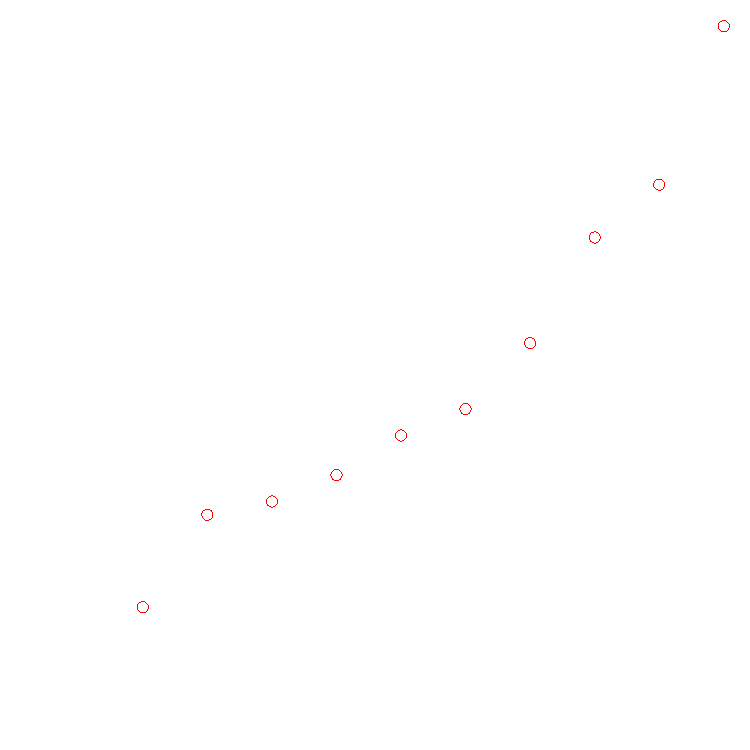
\includegraphics[width=\maxwidth]{figure/graphics-unnamed-chunk-118-1} 

}



\end{knitrout}
\caption{Rette di regressione. In blu $R_x$, in verde $R_y$.}
\label{fig:duerettex}
\end{figure}
\end{center}

\subsubsection{I bambini di Kalama (Egitto). Ancora retta di regressione}
Da DASL \cite{DASL} possiamo scaricare un \emph{dataset} in cui i ricercatori hanno misurato le altezze (cm) dai 18 ai 29 mesi di vita, di 161 bambini di Kalama, un villaggio egiziano. Le altezze sono state mediate tra i bambini per fornire un singolo valore mese per mese.
\begin{knitrout}
\definecolor{shadecolor}{rgb}{0.969, 0.969, 0.969}\color{fgcolor}\begin{kframe}
\begin{alltt}
\hlstd{age}\hlkwb{=}\hlnum{18}\hlopt{:}\hlnum{29}
\hlstd{height}\hlkwb{=}\hlkwd{c}\hlstd{(}\hlnum{76.1}\hlstd{,}\hlnum{77}\hlstd{,}\hlnum{78.1}\hlstd{,}\hlnum{78.2}\hlstd{,}\hlnum{78.8}\hlstd{,}\hlnum{79.7}\hlstd{,}\hlnum{79.9}\hlstd{,}\hlnum{81.1}\hlstd{,}\hlnum{81.2}\hlstd{,}\hlnum{81.8}\hlstd{,}\hlnum{82.8}\hlstd{,}\hlnum{83.5}\hlstd{)}
\end{alltt}
\end{kframe}
\end{knitrout}
Possiamo quindi costruire il \texttt{data.frame}
\begin{knitrout}
\definecolor{shadecolor}{rgb}{0.969, 0.969, 0.969}\color{fgcolor}\begin{kframe}
\begin{alltt}
\hlstd{village}\hlkwb{=}\hlkwd{data.frame}\hlstd{(}\hlkwc{age}\hlstd{=age,}\hlkwc{height}\hlstd{=height)}
\end{alltt}
\end{kframe}
\end{knitrout}
Ora diamo una prima occhiata ai dati:
 %code chunk
\begin{figure}[htbp]
\begin{center}
\begin{knitrout}
\definecolor{shadecolor}{rgb}{0.969, 0.969, 0.969}\color{fgcolor}\begin{kframe}
\begin{alltt}
\hlkwd{plot}\hlstd{(age,height)}
\end{alltt}


{\ttfamily\noindent\bfseries\color{errorcolor}{\#\# Error in getMetricsFromLatex(TeXMetrics, verbose = verbose): \\\#\# TeX was unable to calculate metrics for the following string\\\#\# or character:\\\#\# \\\#\# 	m\\\#\# \\\#\# Common reasons for failure include:\\\#\#\ \  * The string contains a character which is special to LaTeX unless\\\#\#\ \ \ \  escaped properly, such as \% or \$.\\\#\#\ \  * The string makes use of LaTeX commands provided by a package and\\\#\#\ \ \ \  the tikzDevice was not told to load the package.\\\#\# \\\#\# The contents of the LaTeX log of the aborted run have been printed above,\\\#\# it may contain additional details as to why the metric calculation failed.}}\end{kframe}

{\centering 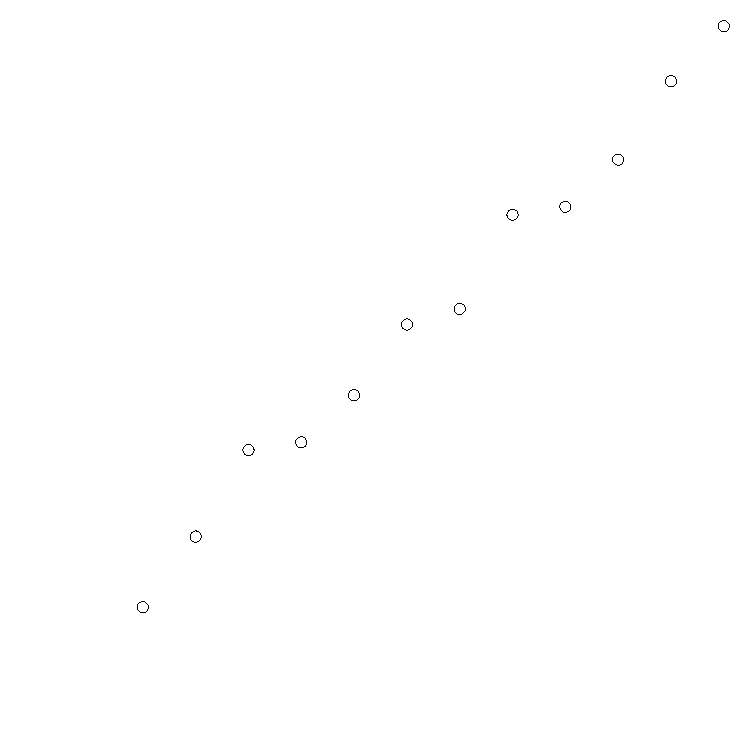
\includegraphics[width=\maxwidth]{figure/graphics-unnamed-chunk-121-1} 

}



\end{knitrout}
\caption{Crescita dei bambini di Kalama}
\label{kalama}
\end{center}
\end{figure}
L'andamento \`e lineare. Determiniamo la retta di regressione
per predire l'altezza media nota l'et\`a in mesi.
%code chunk
\begin{knitrout}
\definecolor{shadecolor}{rgb}{0.969, 0.969, 0.969}\color{fgcolor}\begin{kframe}
\begin{alltt}
\hlstd{(modello}\hlkwb{=}\hlkwd{lm}\hlstd{(height}\hlopt{~}\hlstd{age))}
\end{alltt}
\begin{verbatim}
## 
## Call:
## lm(formula = height ~ age)
## 
## Coefficients:
## (Intercept)          age  
##      64.928        0.635
\end{verbatim}
\end{kframe}
\end{knitrout}
La retta di regressione cercata ha formula:
$$h(\texttt{age})=64.93+ 0.63\, \texttt{age}$$

Possiamo ora utilizzare \textsf{R} come semplice calcolatore per predire l'altezza a 27.5 mesi di et\`a:
oppure, \`e pi\`u  efficiente utilizzare direttamente il \emph{dataframe} e la funzione
\texttt{predict}:
%codechunk
\begin{knitrout}
\definecolor{shadecolor}{rgb}{0.969, 0.969, 0.969}\color{fgcolor}\begin{kframe}
\begin{alltt}
\hlkwd{predict}\hlstd{(modello,}\hlkwd{data.frame}\hlstd{(}\hlkwc{age}\hlstd{=}\hlnum{27.5}\hlstd{))}
\end{alltt}
\begin{verbatim}
##        1 
## 82.38986
\end{verbatim}
\end{kframe}
\end{knitrout}
fornendo in input i parametri della retta ed un preciso valore della variabile indipendente (richiamata col proprio nome).
Molti comandi di \textsf{R} sono in grado di manipolare \emph{dataframe}  lavorando direttamente sulla struttura. Per esempio, il comando plot di un \texttt{dataframe} in due colonne, esegue in automatico il grafico della seconda colonna (variabile dipendente) vs prima colonna (variabile indipendente).
Possiamo ottenere il modello lineare visto nel caso precedente, passando \texttt{village} direttamente al comando:
\begin{knitrout}
\definecolor{shadecolor}{rgb}{0.969, 0.969, 0.969}\color{fgcolor}\begin{kframe}
\begin{alltt}
\hlstd{modello}\hlkwb{=}\hlkwd{lm}\hlstd{(height}\hlopt{~}\hlstd{age,}\hlkwc{data}\hlstd{=village)}
\hlstd{modello}
\end{alltt}
\begin{verbatim}
## 
## Call:
## lm(formula = height ~ age, data = village)
## 
## Coefficients:
## (Intercept)          age  
##      64.928        0.635
\end{verbatim}
\end{kframe}
\end{knitrout}
con la formula \texttt{lm(y \mytilde x,data=dataset)}.
%Inoltre possiamo considerare il plot di un oggetto \texttt{lm}  che fornisce una serie di rappresentazioni grafiche
%<<fig=TRUE,echo=FALSE>>=
%oldpar<-par(mfrow=c(2,2))
%par(ask=FALSE)
%plot(lm(height~age))
%oldpar
%@
\section{Modelli potenza}
Consideriamo ora il seguente \emph{dataset} di mammiferi  in cui le 2 variabili rappresentano  le dimensioni del corpo e del cervello.
\begin{knitrout}
\definecolor{shadecolor}{rgb}{0.969, 0.969, 0.969}\color{fgcolor}\begin{kframe}
\begin{alltt}
\hlkwd{library}\hlstd{(MASS)}
\end{alltt}


{\ttfamily\noindent\itshape\color{messagecolor}{\#\# \\\#\# Attaching package: 'MASS'}}

{\ttfamily\noindent\itshape\color{messagecolor}{\#\# The following object is masked from 'package:EsamiR':\\\#\# \\\#\#\ \ \ \  crabs}}\begin{alltt}
\hlstd{mammals}
\end{alltt}
\begin{verbatim}
##                               body   brain
## Arctic fox                   3.385   44.50
## Owl monkey                   0.480   15.50
## Mountain beaver              1.350    8.10
## Cow                        465.000  423.00
## Grey wolf                   36.330  119.50
## Goat                        27.660  115.00
## Roe deer                    14.830   98.20
## Guinea pig                   1.040    5.50
## Verbet                       4.190   58.00
## Chinchilla                   0.425    6.40
## Ground squirrel              0.101    4.00
## Arctic ground squirrel       0.920    5.70
## African giant pouched rat    1.000    6.60
## Lesser short-tailed shrew    0.005    0.14
## Star-nosed mole              0.060    1.00
## Nine-banded armadillo        3.500   10.80
## Tree hyrax                   2.000   12.30
## N.A. opossum                 1.700    6.30
## Asian elephant            2547.000 4603.00
## Big brown bat                0.023    0.30
## Donkey                     187.100  419.00
## Horse                      521.000  655.00
## European hedgehog            0.785    3.50
## Patas monkey                10.000  115.00
## Cat                          3.300   25.60
## Galago                       0.200    5.00
## Genet                        1.410   17.50
## Giraffe                    529.000  680.00
## Gorilla                    207.000  406.00
## Grey seal                   85.000  325.00
## Rock hyrax-a                 0.750   12.30
## Human                       62.000 1320.00
## African elephant          6654.000 5712.00
## Water opossum                3.500    3.90
## Rhesus monkey                6.800  179.00
## Kangaroo                    35.000   56.00
## Yellow-bellied marmot        4.050   17.00
## Golden hamster               0.120    1.00
## Mouse                        0.023    0.40
## Little brown bat             0.010    0.25
## Slow loris                   1.400   12.50
## Okapi                      250.000  490.00
## Rabbit                       2.500   12.10
## Sheep                       55.500  175.00
## Jaguar                     100.000  157.00
## Chimpanzee                  52.160  440.00
## Baboon                      10.550  179.50
## Desert hedgehog              0.550    2.40
## Giant armadillo             60.000   81.00
## Rock hyrax-b                 3.600   21.00
## Raccoon                      4.288   39.20
## Rat                          0.280    1.90
## E. American mole             0.075    1.20
## Mole rat                     0.122    3.00
## Musk shrew                   0.048    0.33
## Pig                        192.000  180.00
## Echidna                      3.000   25.00
## Brazilian tapir            160.000  169.00
## Tenrec                       0.900    2.60
## Phalanger                    1.620   11.40
## Tree shrew                   0.104    2.50
## Red fox                      4.235   50.40
\end{verbatim}
\end{kframe}
\end{knitrout}
Per prima cosa tracciamo il grafico dei punti  in scala non trasformata e, visto la compresenza di dati molto prossimi all'origine e di dati molto distanti in scala logaritmica (sia le $x$ che le $y$ vengono trasformate prendendone i logaritmi)
\begin{knitrout}
\definecolor{shadecolor}{rgb}{0.969, 0.969, 0.969}\color{fgcolor}\begin{kframe}
\begin{alltt}
\hlkwd{par}\hlstd{(}\hlkwc{mfrow}\hlstd{=}\hlkwd{c}\hlstd{(}\hlnum{1}\hlstd{,}\hlnum{2}\hlstd{))}
\hlkwd{plot}\hlstd{(mammals)}
\end{alltt}


{\ttfamily\noindent\bfseries\color{errorcolor}{\#\# Error in getMetricsFromLatex(TeXMetrics, verbose = verbose): \\\#\# TeX was unable to calculate metrics for the following string\\\#\# or character:\\\#\# \\\#\# 	m\\\#\# \\\#\# Common reasons for failure include:\\\#\#\ \  * The string contains a character which is special to LaTeX unless\\\#\#\ \ \ \  escaped properly, such as \% or \$.\\\#\#\ \  * The string makes use of LaTeX commands provided by a package and\\\#\#\ \ \ \  the tikzDevice was not told to load the package.\\\#\# \\\#\# The contents of the LaTeX log of the aborted run have been printed above,\\\#\# it may contain additional details as to why the metric calculation failed.}}\begin{alltt}
\hlkwd{plot}\hlstd{(mammals,}\hlkwc{log}\hlstd{=}\hlstr{"xy"}\hlstd{)}
\end{alltt}


{\ttfamily\noindent\bfseries\color{errorcolor}{\#\# Error in getMetricsFromLatex(TeXMetrics, verbose = verbose): \\\#\# TeX was unable to calculate metrics for the following string\\\#\# or character:\\\#\# \\\#\# 	m\\\#\# \\\#\# Common reasons for failure include:\\\#\#\ \  * The string contains a character which is special to LaTeX unless\\\#\#\ \ \ \  escaped properly, such as \% or \$.\\\#\#\ \  * The string makes use of LaTeX commands provided by a package and\\\#\#\ \ \ \  the tikzDevice was not told to load the package.\\\#\# \\\#\# The contents of the LaTeX log of the aborted run have been printed above,\\\#\# it may contain additional details as to why the metric calculation failed.}}\end{kframe}
\end{knitrout}
come in Figura~\ref{fig:duemammals}.\begin{figure}[htbp]
\begin{center}
\begin{knitrout}
\definecolor{shadecolor}{rgb}{0.969, 0.969, 0.969}\color{fgcolor}\begin{kframe}


{\ttfamily\noindent\bfseries\color{errorcolor}{\#\# Error in getMetricsFromLatex(TeXMetrics, verbose = verbose): \\\#\# TeX was unable to calculate metrics for the following string\\\#\# or character:\\\#\# \\\#\# 	m\\\#\# \\\#\# Common reasons for failure include:\\\#\#\ \  * The string contains a character which is special to LaTeX unless\\\#\#\ \ \ \  escaped properly, such as \% or \$.\\\#\#\ \  * The string makes use of LaTeX commands provided by a package and\\\#\#\ \ \ \  the tikzDevice was not told to load the package.\\\#\# \\\#\# The contents of the LaTeX log of the aborted run have been printed above,\\\#\# it may contain additional details as to why the metric calculation failed.}}

{\ttfamily\noindent\bfseries\color{errorcolor}{\#\# Error in getMetricsFromLatex(TeXMetrics, verbose = verbose): \\\#\# TeX was unable to calculate metrics for the following string\\\#\# or character:\\\#\# \\\#\# 	m\\\#\# \\\#\# Common reasons for failure include:\\\#\#\ \  * The string contains a character which is special to LaTeX unless\\\#\#\ \ \ \  escaped properly, such as \% or \$.\\\#\#\ \  * The string makes use of LaTeX commands provided by a package and\\\#\#\ \ \ \  the tikzDevice was not told to load the package.\\\#\# \\\#\# The contents of the LaTeX log of the aborted run have been printed above,\\\#\# it may contain additional details as to why the metric calculation failed.}}\end{kframe}

{\centering 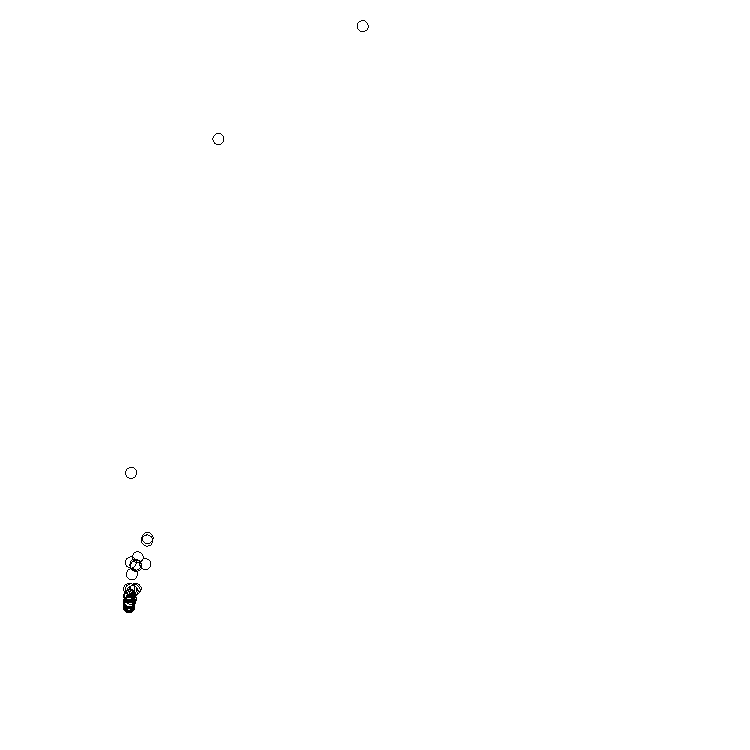
\includegraphics[width=\maxwidth]{figure/graphics-unnamed-chunk-127-1} 

}



\end{knitrout}
\caption{Diagramma a dispersione massa corporea/massa del cervello in scala normale ed in scala logaritmica. }
\label{fig:duemammals}
\end{center}
\end{figure}
Visti i  risultati ottenuti usando la scala logaritmica tracciamo anche la corrispondente retta di regressione
\begin{knitrout}
\definecolor{shadecolor}{rgb}{0.969, 0.969, 0.969}\color{fgcolor}\begin{kframe}
\begin{alltt}
\hlkwd{plot}\hlstd{(}\hlkwd{log}\hlstd{(mammals}\hlopt{$}\hlstd{brain)}\hlopt{~}\hlkwd{log}\hlstd{(mammals}\hlopt{$}\hlstd{body),}\hlkwc{col}\hlstd{=}\hlstr{"BLUE"}\hlstd{,}\hlkwc{pch}\hlstd{=}\hlnum{19}\hlstd{,}\hlkwc{type}\hlstd{=}\hlstr{"p"}\hlstd{)}
\end{alltt}


{\ttfamily\noindent\bfseries\color{errorcolor}{\#\# Error in getMetricsFromLatex(TeXMetrics, verbose = verbose): \\\#\# TeX was unable to calculate metrics for the following string\\\#\# or character:\\\#\# \\\#\# 	m\\\#\# \\\#\# Common reasons for failure include:\\\#\#\ \  * The string contains a character which is special to LaTeX unless\\\#\#\ \ \ \  escaped properly, such as \% or \$.\\\#\#\ \  * The string makes use of LaTeX commands provided by a package and\\\#\#\ \ \ \  the tikzDevice was not told to load the package.\\\#\# \\\#\# The contents of the LaTeX log of the aborted run have been printed above,\\\#\# it may contain additional details as to why the metric calculation failed.}}\begin{alltt}
\hlkwd{abline}\hlstd{(}\hlkwd{lm}\hlstd{(}\hlkwd{log}\hlstd{(mammals}\hlopt{$}\hlstd{brain)}\hlopt{~} \hlkwd{log}\hlstd{(mammals}\hlopt{$}\hlstd{body)),}\hlkwc{col}\hlstd{=}\hlstr{"red"}\hlstd{,}\hlkwc{lwd}\hlstd{=}\hlnum{3}\hlstd{);}
\hlstd{uomo}\hlkwb{=}\hlkwd{which}\hlstd{(}\hlkwd{rownames}\hlstd{(mammals)}\hlopt{==}\hlstr{"Human"}\hlstd{)}
\hlkwd{text}\hlstd{(}\hlkwd{log}\hlstd{(mammals[uomo ,}\hlnum{1}\hlstd{]),}\hlkwd{log}\hlstd{(mammals[uomo ,}\hlnum{2}\hlstd{]),}\hlkwd{rownames}\hlstd{(mammals)[uomo])}
\end{alltt}


{\ttfamily\noindent\bfseries\color{errorcolor}{\#\# Error in getMetricsFromLatex(TeXMetrics, verbose = verbose): \\\#\# TeX was unable to calculate metrics for the following string\\\#\# or character:\\\#\# \\\#\# 	Human\\\#\# \\\#\# Common reasons for failure include:\\\#\#\ \  * The string contains a character which is special to LaTeX unless\\\#\#\ \ \ \  escaped properly, such as \% or \$.\\\#\#\ \  * The string makes use of LaTeX commands provided by a package and\\\#\#\ \ \ \  the tikzDevice was not told to load the package.\\\#\# \\\#\# The contents of the LaTeX log of the aborted run have been printed above,\\\#\# it may contain additional details as to why the metric calculation failed.}}\end{kframe}

{\centering 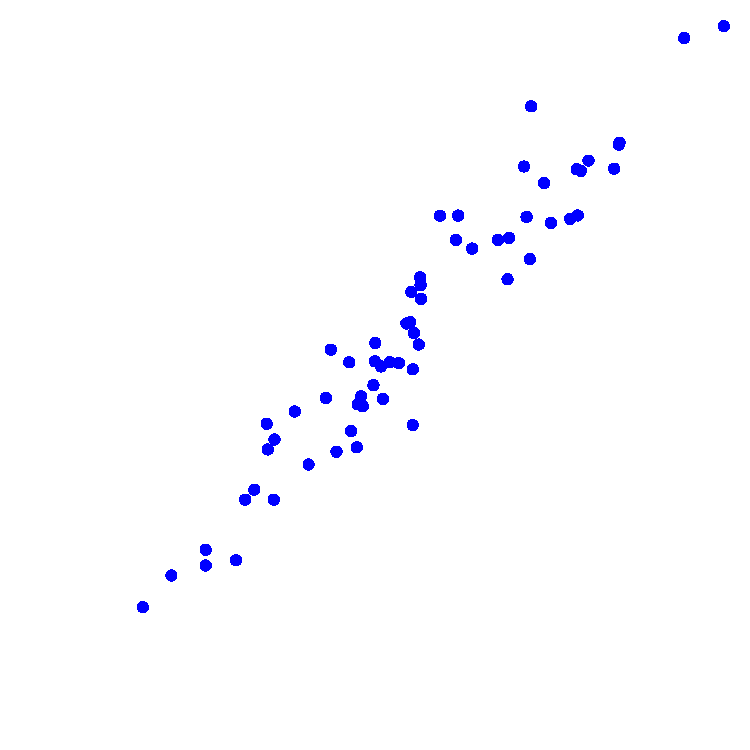
\includegraphics[width=\maxwidth]{figure/graphics-unnamed-chunk-128-1} 

}



\end{knitrout}

\begin{figure}
\begin{center}
\begin{knitrout}
\definecolor{shadecolor}{rgb}{0.969, 0.969, 0.969}\color{fgcolor}\begin{kframe}
\begin{alltt}
\hlkwd{plot}\hlstd{(}\hlkwd{log}\hlstd{(mammals}\hlopt{$}\hlstd{brain)}\hlopt{~}\hlkwd{log}\hlstd{(mammals}\hlopt{$}\hlstd{body),}\hlkwc{col}\hlstd{=}\hlstr{"BLUE"}\hlstd{,}\hlkwc{pch}\hlstd{=}\hlnum{19}\hlstd{,}\hlkwc{type}\hlstd{=}\hlstr{"p"}\hlstd{)}
\end{alltt}


{\ttfamily\noindent\bfseries\color{errorcolor}{\#\# Error in getMetricsFromLatex(TeXMetrics, verbose = verbose): \\\#\# TeX was unable to calculate metrics for the following string\\\#\# or character:\\\#\# \\\#\# 	m\\\#\# \\\#\# Common reasons for failure include:\\\#\#\ \  * The string contains a character which is special to LaTeX unless\\\#\#\ \ \ \  escaped properly, such as \% or \$.\\\#\#\ \  * The string makes use of LaTeX commands provided by a package and\\\#\#\ \ \ \  the tikzDevice was not told to load the package.\\\#\# \\\#\# The contents of the LaTeX log of the aborted run have been printed above,\\\#\# it may contain additional details as to why the metric calculation failed.}}\begin{alltt}
\hlkwd{abline}\hlstd{(}\hlkwd{lm}\hlstd{(}\hlkwd{log}\hlstd{(mammals}\hlopt{$}\hlstd{brain)}\hlopt{~} \hlkwd{log}\hlstd{(mammals}\hlopt{$}\hlstd{body)),}\hlkwc{col}\hlstd{=}\hlstr{"red"}\hlstd{,}\hlkwc{lwd}\hlstd{=}\hlnum{3} \hlstd{);}
\hlstd{uomo}\hlkwb{=}\hlkwd{which}\hlstd{(}\hlkwd{rownames}\hlstd{(mammals)}\hlopt{==}\hlstr{"Human"}\hlstd{)}
\hlkwd{text}\hlstd{(} \hlkwd{log}\hlstd{(mammals[uomo ,}\hlnum{1}\hlstd{]),}\hlkwd{log}\hlstd{(mammals[uomo ,}\hlnum{2}\hlstd{]),}\hlkwd{rownames}\hlstd{(mammals)[uomo])}
\end{alltt}


{\ttfamily\noindent\bfseries\color{errorcolor}{\#\# Error in getMetricsFromLatex(TeXMetrics, verbose = verbose): \\\#\# TeX was unable to calculate metrics for the following string\\\#\# or character:\\\#\# \\\#\# 	Human\\\#\# \\\#\# Common reasons for failure include:\\\#\#\ \  * The string contains a character which is special to LaTeX unless\\\#\#\ \ \ \  escaped properly, such as \% or \$.\\\#\#\ \  * The string makes use of LaTeX commands provided by a package and\\\#\#\ \ \ \  the tikzDevice was not told to load the package.\\\#\# \\\#\# The contents of the LaTeX log of the aborted run have been printed above,\\\#\# it may contain additional details as to why the metric calculation failed.}}\end{kframe}

{\centering 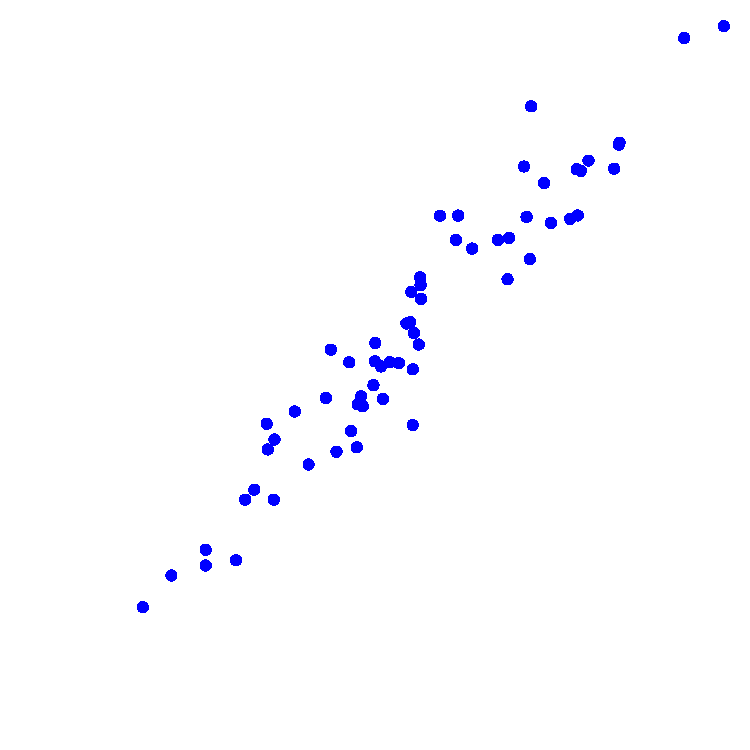
\includegraphics[width=\maxwidth]{figure/graphics-ddd-1} 

}



\end{knitrout}
\caption{ Retta di regressione. Dimensione del corpo e del cervello. Si noti la posizione dell'uomo.}
\label{duerette}
\end{center}
\end{figure}
Si noti il comando \texttt{text(\varia{x},\varia{y}, \varia{testo})}
dove    $\varia{x}$ e $\varia{y}$  e $\varia{testo}$ sono vettori di arbitraria lunghezza contenenti ascisse, ordinate e testo da inserire.
\section{Distribuzioni in \textsf{R}}
I nomi delle principali distribuzioni in \textsf{R} sono\vskip10pt
\begin{tabular}{|r|c |}
\hline
\texttt{norm}&normale\\
\texttt{t}  &Student\\
\texttt{chisq}& chi quadro\\
\texttt{f}&Fisher\\
\texttt{binom }&binomiale\\
\hline
\end{tabular}\vskip10pt
A questi nomi possiamo aggiungere diversi prefissi\vskip10pt
\begin{tabular}{|r|c |}
\hline
\texttt{d}&densit\`a\\
\texttt{p}  &primitiva\\
\texttt{q}& quantile\\
\texttt{r}&random\\
  \hline
\end{tabular}
\vskip10pt
per caratterizzare diversi aspetti.
\begin{comment}
\begin{knitrout}
\definecolor{shadecolor}{rgb}{0.969, 0.969, 0.969}\color{fgcolor}\begin{kframe}


{\ttfamily\noindent\color{warningcolor}{\#\# Warning in sqrt(1 - r\textasciicircum{}2): NaNs produced}}

{\ttfamily\noindent\color{warningcolor}{\#\# Warning in rnorm(200, a, sy * sqrt(1 - r\textasciicircum{}2)): NAs produced}}

{\ttfamily\noindent\color{warningcolor}{\#\# Warning in solutions[1] <- abs(b - 1) < 0.1: number of items to replace is not a multiple of replacement length}}

{\ttfamily\noindent\color{warningcolor}{\#\# Warning in explanations[1] <- paste("{}The slope of the regression line is given by \$r \textbackslash{}\textbackslash{}\textbackslash{}\textbackslash{}cdot s\_y/s\_x\$ and hence"{}, : number of items to replace is not a multiple of replacement length}}

{\ttfamily\noindent\color{warningcolor}{\#\# Warning in solutions[2] <- abs(r) <= 0.8: number of items to replace is not a multiple of replacement length}}

{\ttfamily\noindent\color{warningcolor}{\#\# Warning in if (abs(r) >= 0.9) \{: the condition has length > 1 and only the first element will be used}}

{\ttfamily\noindent\color{warningcolor}{\#\# Warning in if (abs(r) > 0 \& abs(mx - xh) > 0) sign(mx - xh) * sign(r) else 1: the condition has length > 1 and only the first element will be used}}

{\ttfamily\noindent\color{warningcolor}{\#\# Warning in solutions[5] <- abs(yh - yhr) < 0.01 * sy: number of items to replace is not a multiple of replacement length}}

{\ttfamily\noindent\color{warningcolor}{\#\# Warning in explanations[5] <- paste("{}The regression line at \$X="{}, xh, "{}\$ implies a value of about \$Y = "{}, : number of items to replace is not a multiple of replacement length}}\end{kframe}
\end{knitrout}
\begin{itemize}
\begin{question}
  Figure~\ref{fig:scatterplot} shows a scatterplot. Which of the
  following statements are correct?


\begin{figure}[htb!]
\begin{center}
\begin{knitrout}
\definecolor{shadecolor}{rgb}{0.969, 0.969, 0.969}\color{fgcolor}\begin{kframe}


{\ttfamily\noindent\bfseries\color{errorcolor}{\#\# Error in getMetricsFromLatex(TeXMetrics, verbose = verbose): \\\#\# TeX was unable to calculate metrics for the following string\\\#\# or character:\\\#\# \\\#\# 	m\\\#\# \\\#\# Common reasons for failure include:\\\#\#\ \  * The string contains a character which is special to LaTeX unless\\\#\#\ \ \ \  escaped properly, such as \% or \$.\\\#\#\ \  * The string makes use of LaTeX commands provided by a package and\\\#\#\ \ \ \  the tikzDevice was not told to load the package.\\\#\# \\\#\# The contents of the LaTeX log of the aborted run have been printed above,\\\#\# it may contain additional details as to why the metric calculation failed.}}\end{kframe}

{\centering 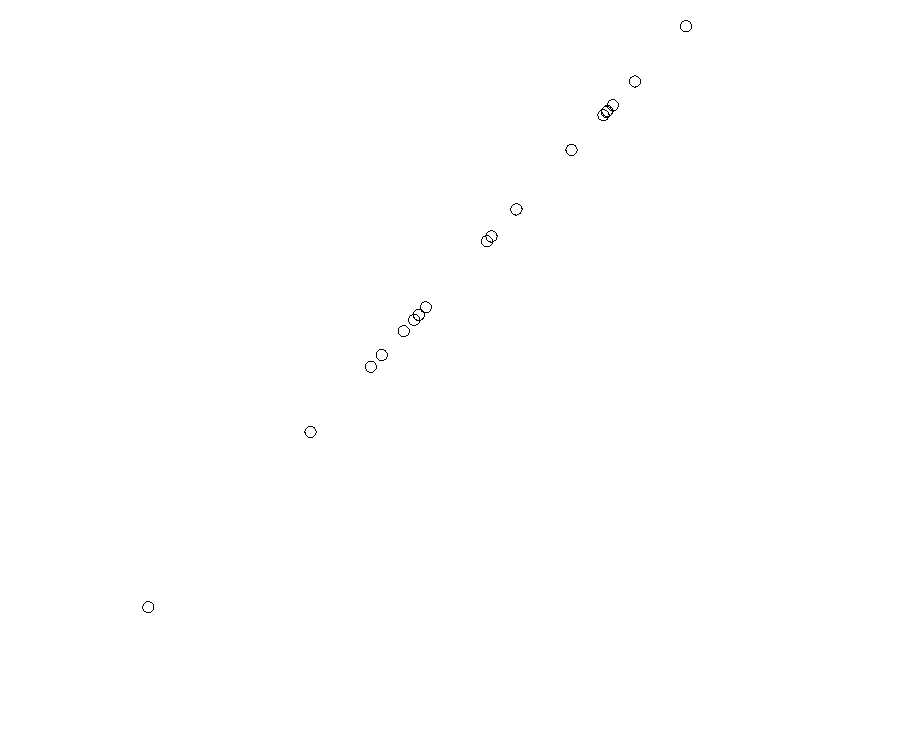
\includegraphics[width=\maxwidth]{figure/graphics-unnamed-chunk-130-1} 

}



\end{knitrout}
\caption{ Scatterplot}\label{fig:scatterplot}
\end{center}
\end{figure}

\begin{answerlist}
  \item The standard deviation of $Y$ is at least $6$.
  \item For $X =  13.6 $, $Y$ can be expected to be about  -44 .
  \item La pendenza della retta di regressione ? circa $1$.
  \item The mean of $X$ is at most $5$.
  \item The absolute value of the correlation coefficient is at most $0.8$.
\end{answerlist}
\end{question}

%% SOLUTIONS
\begin{solution}
\begin{answerlist}
  \item \\textbf{True}: The standard deviation of $Y$ is about equal to $ 20 $ and is therefore larger than $6$.
  \item \\textbf{False}: The regression line at $X=13.6$ implies a value of about $Y = 7.2$.
  \item \\textbf{False}: The slope of the regression line is given by $r \\cdot s_y/s_x$ and hence not about equal to $1$.
  \item \\textbf{False}: The mean of $X$ is about equal to $ 20 $ and hence is larger than $5$.
  \item \\textbf{False}: A strong association between the variables is given in the scatterplot. Hence the absolute value of the correlation coefficient is close to $1$ and therefore larger than $0.8$.
\end{answerlist}
\end{solution}
\end{itemize}
%% META-INFORMATION
%% \extype{mchoice}
%% \exsolution{mchoice2string(solutions)}
%% \exname{Multiple choice}

\end{comment}
\subsection{Distribuzione normale}
\subsubsection{La funzione \texttt{dnorm}}
Come appena visto \textsf{R }indica con il nome \texttt{dnorm}, la densit\`a normale o gaussiana. Essa accetta come parametri sia la media $\mu$ che la deviazione standard $\sigma$ come \`e possibile verificare con il comando \texttt{formals} che ci fornisce gli argomenti di una funzione e gli eventuali valori preassegnati.
\begin{knitrout}
\definecolor{shadecolor}{rgb}{0.969, 0.969, 0.969}\color{fgcolor}\begin{kframe}
\begin{alltt}
\hlkwd{formals}\hlstd{(dnorm)}
\end{alltt}
\begin{verbatim}
## $x
## 
## 
## $mean
## [1] 0
## 
## $sd
## [1] 1
## 
## $log
## [1] FALSE
\end{verbatim}
\end{kframe}
\end{knitrout}
Se i parametri sono omessi \texttt{dnorm} rappresenta la densit\`a normale standard con $\mu=0$ e $\sigma=1$.
Il grafico~(\ref{fig:normalesta}) della gaussiana
 tra due estremi, ad esempio -2.5 e 2.5 si ottiene con il solito comando
\begin{knitrout}
\definecolor{shadecolor}{rgb}{0.969, 0.969, 0.969}\color{fgcolor}\begin{kframe}
\begin{alltt}
\hlkwd{curve}\hlstd{(dnorm,}\hlopt{-}\hlnum{2.5}\hlstd{,}\hlnum{2.5}\hlstd{)}
\end{alltt}


{\ttfamily\noindent\bfseries\color{errorcolor}{\#\# Error in getMetricsFromLatex(TeXMetrics, verbose = verbose): \\\#\# TeX was unable to calculate metrics for the following string\\\#\# or character:\\\#\# \\\#\# 	m\\\#\# \\\#\# Common reasons for failure include:\\\#\#\ \  * The string contains a character which is special to LaTeX unless\\\#\#\ \ \ \  escaped properly, such as \% or \$.\\\#\#\ \  * The string makes use of LaTeX commands provided by a package and\\\#\#\ \ \ \  the tikzDevice was not told to load the package.\\\#\# \\\#\# The contents of the LaTeX log of the aborted run have been printed above,\\\#\# it may contain additional details as to why the metric calculation failed.}}\end{kframe}
\end{knitrout}

\begin{figure}[htbp]
\begin{center}
\begin{knitrout}
\definecolor{shadecolor}{rgb}{0.969, 0.969, 0.969}\color{fgcolor}\begin{kframe}


{\ttfamily\noindent\bfseries\color{errorcolor}{\#\# Error in getMetricsFromLatex(TeXMetrics, verbose = verbose): \\\#\# TeX was unable to calculate metrics for the following string\\\#\# or character:\\\#\# \\\#\# 	m\\\#\# \\\#\# Common reasons for failure include:\\\#\#\ \  * The string contains a character which is special to LaTeX unless\\\#\#\ \ \ \  escaped properly, such as \% or \$.\\\#\#\ \  * The string makes use of LaTeX commands provided by a package and\\\#\#\ \ \ \  the tikzDevice was not told to load the package.\\\#\# \\\#\# The contents of the LaTeX log of the aborted run have been printed above,\\\#\# it may contain additional details as to why the metric calculation failed.}}\end{kframe}

{\centering 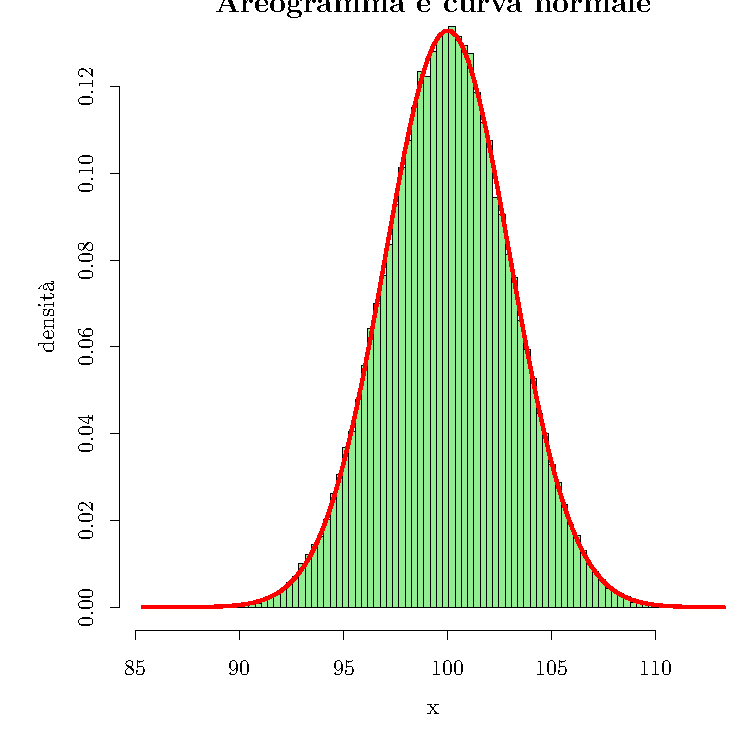
\includegraphics[width=\maxwidth]{figure/graphics-unnamed-chunk-133-1} 

}



\end{knitrout}
\caption{ Grafico della normale standard nell'intervallo $[-2.5,2.5]$. }
\label{fig:normalesta}
\end{center}
\end{figure}
Per  visualizzare una gaussiana non standard, ad esempio una gaussiana con media $\mu=1$ e  deviazione standard $\sigma=1.5$, tra -3 e 3. scriveremo invece
\begin{knitrout}
\definecolor{shadecolor}{rgb}{0.969, 0.969, 0.969}\color{fgcolor}\begin{kframe}
\begin{alltt}
\hlkwd{curve}\hlstd{(}\hlkwd{dnorm}\hlstd{(x,}\hlkwc{mean}\hlstd{=}\hlnum{1}\hlstd{,}\hlkwc{sd}\hlstd{=}\hlnum{1.5}\hlstd{),}\hlopt{-}\hlnum{3}\hlstd{,}\hlnum{3}\hlstd{)}
\end{alltt}


{\ttfamily\noindent\bfseries\color{errorcolor}{\#\# Error in getMetricsFromLatex(TeXMetrics, verbose = verbose): \\\#\# TeX was unable to calculate metrics for the following string\\\#\# or character:\\\#\# \\\#\# 	m\\\#\# \\\#\# Common reasons for failure include:\\\#\#\ \  * The string contains a character which is special to LaTeX unless\\\#\#\ \ \ \  escaped properly, such as \% or \$.\\\#\#\ \  * The string makes use of LaTeX commands provided by a package and\\\#\#\ \ \ \  the tikzDevice was not told to load the package.\\\#\# \\\#\# The contents of the LaTeX log of the aborted run have been printed above,\\\#\# it may contain additional details as to why the metric calculation failed.}}\end{kframe}

{\centering 
\includegraphics[width=\maxwidth]{figure/graphics-unnamed-chunk-134-1} 

}



\end{knitrout}
\subsection{La funzione \texttt{pnorm}}
La funzione \texttt{pnorm}(\varia{x})   \`e la antiderivata di \texttt{dnorm} calcolata come segue
\begin{equation*}\texttt{pnorm}(\varia{x}) =\int_{-\infty}^x  \texttt{dnorm}(s)ds
\end{equation*}
Ovviamente
$$\int_a^b \texttt{dnorm}(x)dx=\texttt{pnorm}(b)-\texttt{pnorm}(a)$$
e per avere l'area sottesa tra $3$ e $5$  basta scrivere:
\begin{knitrout}
\definecolor{shadecolor}{rgb}{0.969, 0.969, 0.969}\color{fgcolor}\begin{kframe}
\begin{alltt}
\hlkwd{pnorm}\hlstd{(}\hlnum{5}\hlstd{)}\hlopt{-}\hlkwd{pnorm}\hlstd{(}\hlnum{3}\hlstd{)}
\end{alltt}
\begin{verbatim}
## [1] 0.001349611
\end{verbatim}
\end{kframe}
\end{knitrout}

Per ottenere il valore dell'area tra 0 e $x$ bisogna allora sottrarre \texttt{pnorm}(0)=0.5 all'area fornita dalla funzione.
Per cui possiamo scrivere:
\begin{knitrout}
\definecolor{shadecolor}{rgb}{0.969, 0.969, 0.969}\color{fgcolor}\begin{kframe}
\begin{alltt}
\hlkwd{pnorm}\hlstd{(}\hlnum{1}\hlstd{)}\hlopt{-}\hlnum{0.5}
\end{alltt}
\begin{verbatim}
## [1] 0.3413447
\end{verbatim}
\end{kframe}
\end{knitrout}


\subsection{La funzione \texttt{qnorm} e la tabella della densit\`a di Gauss}


La funzione \texttt{qnorm} rappresenta la funzione inversa di \texttt{pnorm}.
\[\texttt{qnorm}(A)=x\Leftrightarrow A=\int_{-\infty}^x \texttt{dnorm}(s)ds\] 
come illustrato nella figura~\ref{fig:fig2code}.
\begin{center}
\begin{figure}[H]
\begin{knitrout}
\definecolor{shadecolor}{rgb}{0.969, 0.969, 0.969}\color{fgcolor}\begin{kframe}


{\ttfamily\noindent\bfseries\color{errorcolor}{\#\# Error in getMetricsFromLatex(TeXMetrics, verbose = verbose): \\\#\# TeX was unable to calculate metrics for the following string\\\#\# or character:\\\#\# \\\#\# 	dnorm(x, mu, sigma)\\\#\# \\\#\# Common reasons for failure include:\\\#\#\ \  * The string contains a character which is special to LaTeX unless\\\#\#\ \ \ \  escaped properly, such as \% or \$.\\\#\#\ \  * The string makes use of LaTeX commands provided by a package and\\\#\#\ \ \ \  the tikzDevice was not told to load the package.\\\#\# \\\#\# The contents of the LaTeX log of the aborted run have been printed above,\\\#\# it may contain additional details as to why the metric calculation failed.}}\end{kframe}

{\centering 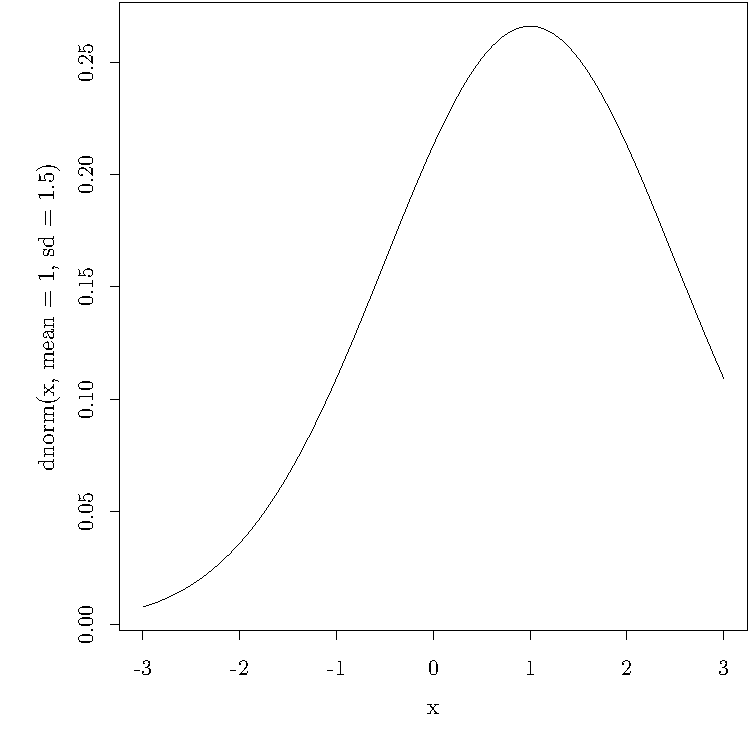
\includegraphics[width=\maxwidth]{figure/graphics-unnamed-chunk-138-1} 

}



\end{knitrout}
\caption{$x=\texttt{qnorm}(A)$}
\label{fig:fig2code}
\end{figure}
\end{center}
Vogliamo costruire una funzione, diciamo $U$ tale che assegnato un valore di area $A$   fornisca l'ascissa $x=U(A)$ come in figura~\ref{fig:fig12code} in modo che l'area tra - $x$ e $x$ sia esattamente pari ad $A$.  

\begin{figure}[H]
\begin{knitrout}
\definecolor{shadecolor}{rgb}{0.969, 0.969, 0.969}\color{fgcolor}\begin{kframe}


{\ttfamily\noindent\bfseries\color{errorcolor}{\#\# Error in getMetricsFromLatex(TeXMetrics, verbose = verbose): \\\#\# TeX was unable to calculate metrics for the following string\\\#\# or character:\\\#\# \\\#\# 	m\\\#\# \\\#\# Common reasons for failure include:\\\#\#\ \  * The string contains a character which is special to LaTeX unless\\\#\#\ \ \ \  escaped properly, such as \% or \$.\\\#\#\ \  * The string makes use of LaTeX commands provided by a package and\\\#\#\ \ \ \  the tikzDevice was not told to load the package.\\\#\# \\\#\# The contents of the LaTeX log of the aborted run have been printed above,\\\#\# it may contain additional details as to why the metric calculation failed.}}

{\ttfamily\noindent\bfseries\color{errorcolor}{\#\# Error in getMetricsFromLatex(TeXMetrics, verbose = verbose): \\\#\# TeX was unable to calculate metrics for the following string\\\#\# or character:\\\#\# \\\#\# 	m\\\#\# \\\#\# Common reasons for failure include:\\\#\#\ \  * The string contains a character which is special to LaTeX unless\\\#\#\ \ \ \  escaped properly, such as \% or \$.\\\#\#\ \  * The string makes use of LaTeX commands provided by a package and\\\#\#\ \ \ \  the tikzDevice was not told to load the package.\\\#\# \\\#\# The contents of the LaTeX log of the aborted run have been printed above,\\\#\# it may contain additional details as to why the metric calculation failed.}}\end{kframe}

{\centering 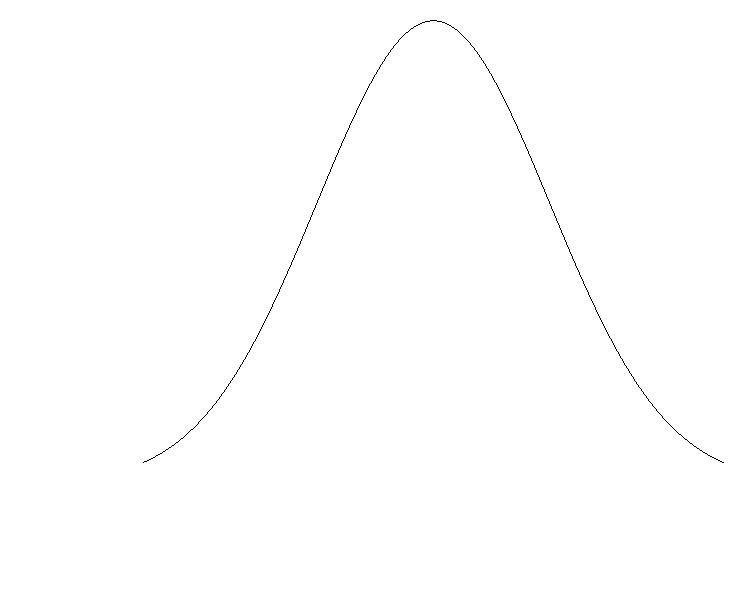
\includegraphics[width=\maxwidth]{figure/graphics-unnamed-chunk-139-1} 

}



\end{knitrout}
\caption{$x=U(A)=\texttt{qnorm}(1/2+A/2)$}
\label{fig:fig12code}
\end{figure}
Dalla stessa figura  si evince che la funzione che riproduce la tabella è
\begin{knitrout}
\definecolor{shadecolor}{rgb}{0.969, 0.969, 0.969}\color{fgcolor}\begin{kframe}
\begin{alltt}
\hlstd{U} \hlkwb{<-}\hlkwa{function} \hlstd{(}\hlkwc{A}\hlstd{)} \hlkwd{qnorm} \hlstd{(}\hlnum{1}\hlopt{/}\hlnum{2} \hlopt{+} \hlstd{A}\hlopt{/}\hlnum{2}\hlstd{)}
\end{alltt}
\end{kframe}
\end{knitrout}
Questa funzione fornisce fissato il livello di fiducia l'ascissa $x$  tale che l'intervallo simmetrico $[-x,x]$ racchiuda un'area pari al lvello di fiducia. Per esempio
\begin{knitrout}
\definecolor{shadecolor}{rgb}{0.969, 0.969, 0.969}\color{fgcolor}\begin{kframe}
\begin{alltt}
\hlkwd{U}\hlstd{(}\hlnum{0.95}\hlstd{)}
\end{alltt}
\begin{verbatim}
## [1] 1.959964
\end{verbatim}
\end{kframe}
\end{knitrout}
\begin{figure}[htbp]
\begin{center}
\begin{knitrout}
\definecolor{shadecolor}{rgb}{0.969, 0.969, 0.969}\color{fgcolor}\begin{kframe}


{\ttfamily\noindent\bfseries\color{errorcolor}{\#\# Error in axis(1, c(-3, -1, 0, 1, 3), c("{}"{}, expression(-u[1 - epsilon]), : plot.new has not been called yet}}\end{kframe}
\end{knitrout}
\begin{knitrout}
\definecolor{shadecolor}{rgb}{0.969, 0.969, 0.969}\color{fgcolor}\begin{kframe}


{\ttfamily\noindent\bfseries\color{errorcolor}{\#\# Error in getMetricsFromLatex(TeXMetrics, verbose = verbose): \\\#\# TeX was unable to calculate metrics for the following string\\\#\# or character:\\\#\# \\\#\# 	m\\\#\# \\\#\# Common reasons for failure include:\\\#\#\ \  * The string contains a character which is special to LaTeX unless\\\#\#\ \ \ \  escaped properly, such as \% or \$.\\\#\#\ \  * The string makes use of LaTeX commands provided by a package and\\\#\#\ \ \ \  the tikzDevice was not told to load the package.\\\#\# \\\#\# The contents of the LaTeX log of the aborted run have been printed above,\\\#\# it may contain additional details as to why the metric calculation failed.}}

{\ttfamily\noindent\bfseries\color{errorcolor}{\#\# Error in getMetricsFromLatex(TeXMetrics, verbose = verbose): \\\#\# TeX was unable to calculate metrics for the following string\\\#\# or character:\\\#\# \\\#\# 	77\\\#\# \\\#\# Common reasons for failure include:\\\#\#\ \  * The string contains a character which is special to LaTeX unless\\\#\#\ \ \ \  escaped properly, such as \% or \$.\\\#\#\ \  * The string makes use of LaTeX commands provided by a package and\\\#\#\ \ \ \  the tikzDevice was not told to load the package.\\\#\# \\\#\# The contents of the LaTeX log of the aborted run have been printed above,\\\#\# it may contain additional details as to why the metric calculation failed.}}

{\ttfamily\noindent\bfseries\color{errorcolor}{\#\# Error in getMetricsFromLatex(TeXMetrics, verbose = verbose): \\\#\# TeX was unable to calculate metrics for the following string\\\#\# or character:\\\#\# \\\#\# 	77\\\#\# \\\#\# Common reasons for failure include:\\\#\#\ \  * The string contains a character which is special to LaTeX unless\\\#\#\ \ \ \  escaped properly, such as \% or \$.\\\#\#\ \  * The string makes use of LaTeX commands provided by a package and\\\#\#\ \ \ \  the tikzDevice was not told to load the package.\\\#\# \\\#\# The contents of the LaTeX log of the aborted run have been printed above,\\\#\# it may contain additional details as to why the metric calculation failed.}}

{\ttfamily\noindent\bfseries\color{errorcolor}{\#\# Error in getMetricsFromLatex(TeXMetrics, verbose = verbose): \\\#\# TeX was unable to calculate metrics for the following string\\\#\# or character:\\\#\# \\\#\# 	77\\\#\# \\\#\# Common reasons for failure include:\\\#\#\ \  * The string contains a character which is special to LaTeX unless\\\#\#\ \ \ \  escaped properly, such as \% or \$.\\\#\#\ \  * The string makes use of LaTeX commands provided by a package and\\\#\#\ \ \ \  the tikzDevice was not told to load the package.\\\#\# \\\#\# The contents of the LaTeX log of the aborted run have been printed above,\\\#\# it may contain additional details as to why the metric calculation failed.}}\end{kframe}

{\centering 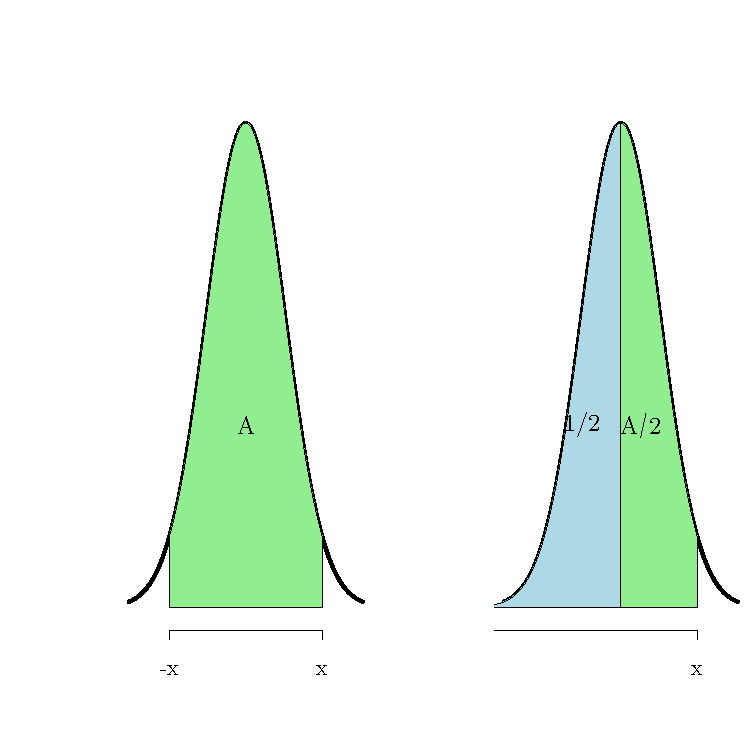
\includegraphics[width=\maxwidth]{figure/graphics-unnamed-chunk-143-1} 

}



\end{knitrout}
\caption{Code della distribuzione normale}
\label{fig:normaletratto}
\end{center}
\end{figure}

 \subsection{La funzione \texttt{rnorm}}
\`E possibile generare dei valori standardizzati casuali (media uguale a 0, deviazione standard pari a 1) che seguono la distribuzione normale standard. Basta semplicemente definire il numero di valori desiderati.
Il comando nella sua espressione generale \`e:
\begin{equation}\texttt{rnorm}(n,\texttt{mean}=\varia{valore}_1,\texttt{sd}=\varia{valore}_2)\end{equation}
Nel caso in cui volessimo una lista di 20 valori di una variabile normale con media assegnata 5 e deviazione standard 1 scriveremo
\begin{knitrout}
\definecolor{shadecolor}{rgb}{0.969, 0.969, 0.969}\color{fgcolor}\begin{kframe}
\begin{alltt}
\hlkwd{rnorm}\hlstd{(}\hlnum{20}\hlstd{,}\hlkwc{mean}\hlstd{=}\hlnum{5}\hlstd{,}\hlkwc{sd}\hlstd{=}\hlnum{1}\hlstd{)}
\end{alltt}
\begin{verbatim}
##  [1] 4.468756 5.062037 5.103530 6.169799 5.394189
##  [6] 4.865898 4.620124 6.278667 4.300668 5.564251
## [11] 5.302942 5.215441 5.921003 4.112448 4.997107
## [16] 4.804826 2.765321 5.478323 6.622692 3.803926
\end{verbatim}
\end{kframe}
\end{knitrout}
\subsection{La distribuzione $t$ di Student}
In \textsf{R} la distribuzione di Student \`e indicata con la lettera  \texttt{t}.  Come per le altre densit\`a  si possono considerare le funzioni\vskip5pt
\begin{tabular}{|r|r |}
\hline
dt  &densit\`a\\
pt  &primitiva\\
qt & quantili\\
rt  &generatore random\\
\hline
\end{tabular}
\vskip10pt
Il grafico della distribuzione di Student ad un certo numero \texttt{df} di gradi di libert\`a  si ottiene con il comando
\begin{equation*}
\texttt{curve(dt(x},\texttt{df}),\varia{a},\varia{b})
\end{equation*}
Tracciamo ad esempio un grafico tra -2 e 2 per una distribuzione a 10 gradi di libert\`a (vedi figura ~(\ref{fig:graficostudent1})):

\begin{figure}[H]
\begin{center}
\begin{knitrout}
\definecolor{shadecolor}{rgb}{0.969, 0.969, 0.969}\color{fgcolor}\begin{kframe}
\begin{alltt}
\hlkwd{curve}\hlstd{(}\hlkwd{dt}\hlstd{(x,}\hlnum{10}\hlstd{),}\hlopt{-}\hlnum{2}\hlstd{,}\hlnum{2}\hlstd{)}
\end{alltt}


{\ttfamily\noindent\bfseries\color{errorcolor}{\#\# Error in getMetricsFromLatex(TeXMetrics, verbose = verbose): \\\#\# TeX was unable to calculate metrics for the following string\\\#\# or character:\\\#\# \\\#\# 	m\\\#\# \\\#\# Common reasons for failure include:\\\#\#\ \  * The string contains a character which is special to LaTeX unless\\\#\#\ \ \ \  escaped properly, such as \% or \$.\\\#\#\ \  * The string makes use of LaTeX commands provided by a package and\\\#\#\ \ \ \  the tikzDevice was not told to load the package.\\\#\# \\\#\# The contents of the LaTeX log of the aborted run have been printed above,\\\#\# it may contain additional details as to why the metric calculation failed.}}\end{kframe}

{\centering 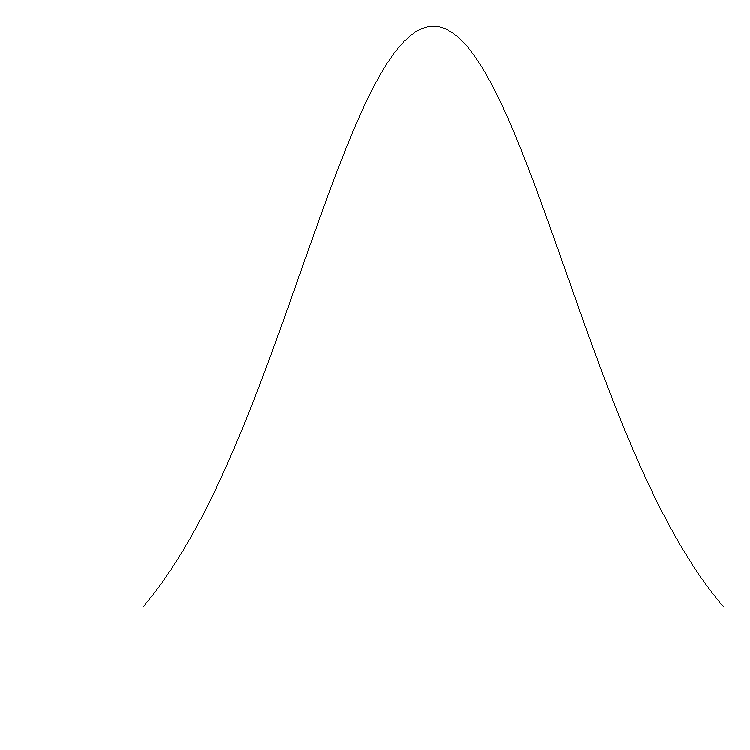
\includegraphics[width=\maxwidth]{figure/graphics-unnamed-chunk-145-1} 

}



\end{knitrout}
\caption{Grafico della distribuzione di Student a 10 gradi di libert\`a. }
\label{fig:graficostudent1}
\end{center}
\end{figure}
Ricordiamo che la distribuzione di Student si usa in  particolare nei casi in cui la deviazione standard della popolazione $\sigma$  non \`e conosciuta e viene rimpiazzata  dalla deviazione standard campionaria  $S$, calcolata con un numero $N$ di dati e quindi con $N-1$ gradi di libert\`a. Quando per\`o il numero di dati si avvicina a 30 la curva di Student \`e praticamente sovrapposta a quella della distribuzione normale, come mostra il grafico~(\ref{fig:graficostudent}):

\begin{figure}[H]
\begin{center}
\begin{knitrout}
\definecolor{shadecolor}{rgb}{0.969, 0.969, 0.969}\color{fgcolor}\begin{kframe}
\begin{alltt}
\hlkwd{curve}\hlstd{(}\hlkwd{dnorm}\hlstd{(x),}\hlopt{-}\hlnum{2}\hlstd{,}\hlnum{2}\hlstd{,}\hlkwc{col}\hlstd{=}\hlnum{3}\hlstd{)}
\end{alltt}


{\ttfamily\noindent\bfseries\color{errorcolor}{\#\# Error in getMetricsFromLatex(TeXMetrics, verbose = verbose): \\\#\# TeX was unable to calculate metrics for the following string\\\#\# or character:\\\#\# \\\#\# 	m\\\#\# \\\#\# Common reasons for failure include:\\\#\#\ \  * The string contains a character which is special to LaTeX unless\\\#\#\ \ \ \  escaped properly, such as \% or \$.\\\#\#\ \  * The string makes use of LaTeX commands provided by a package and\\\#\#\ \ \ \  the tikzDevice was not told to load the package.\\\#\# \\\#\# The contents of the LaTeX log of the aborted run have been printed above,\\\#\# it may contain additional details as to why the metric calculation failed.}}\begin{alltt}
\hlkwd{curve}\hlstd{(}\hlkwd{dt}\hlstd{(x,}\hlnum{2}\hlstd{),}\hlopt{-}\hlnum{2}\hlstd{,}\hlnum{2}\hlstd{,}\hlkwc{col}\hlstd{=}\hlnum{1}\hlstd{,}\hlkwc{add}\hlstd{=T)}
\hlkwd{curve}\hlstd{(}\hlkwd{dt}\hlstd{(x,}\hlnum{25}\hlstd{),}\hlopt{-}\hlnum{2}\hlstd{,}\hlnum{2}\hlstd{,}\hlkwc{col}\hlstd{=}\hlnum{2}\hlstd{,}\hlkwc{add}\hlstd{=T)}
\hlkwd{legend}\hlstd{(}\hlstr{"topleft"}\hlstd{,} \hlkwd{c}\hlstd{(}\hlstr{"df=2"}\hlstd{,}\hlstr{"df=25"}\hlstd{,}\hlstr{"normale"}\hlstd{),}\hlkwc{pch}\hlstd{=}\hlnum{15}\hlstd{,}\hlkwc{col}\hlstd{=}\hlnum{1}\hlopt{:}\hlnum{3}\hlstd{);}
\end{alltt}


{\ttfamily\noindent\bfseries\color{errorcolor}{\#\# Error in getMetricsFromLatex(TeXMetrics, verbose = verbose): \\\#\# TeX was unable to calculate metrics for the following string\\\#\# or character:\\\#\# \\\#\# 	df=2\\\#\# \\\#\# Common reasons for failure include:\\\#\#\ \  * The string contains a character which is special to LaTeX unless\\\#\#\ \ \ \  escaped properly, such as \% or \$.\\\#\#\ \  * The string makes use of LaTeX commands provided by a package and\\\#\#\ \ \ \  the tikzDevice was not told to load the package.\\\#\# \\\#\# The contents of the LaTeX log of the aborted run have been printed above,\\\#\# it may contain additional details as to why the metric calculation failed.}}\end{kframe}

{\centering 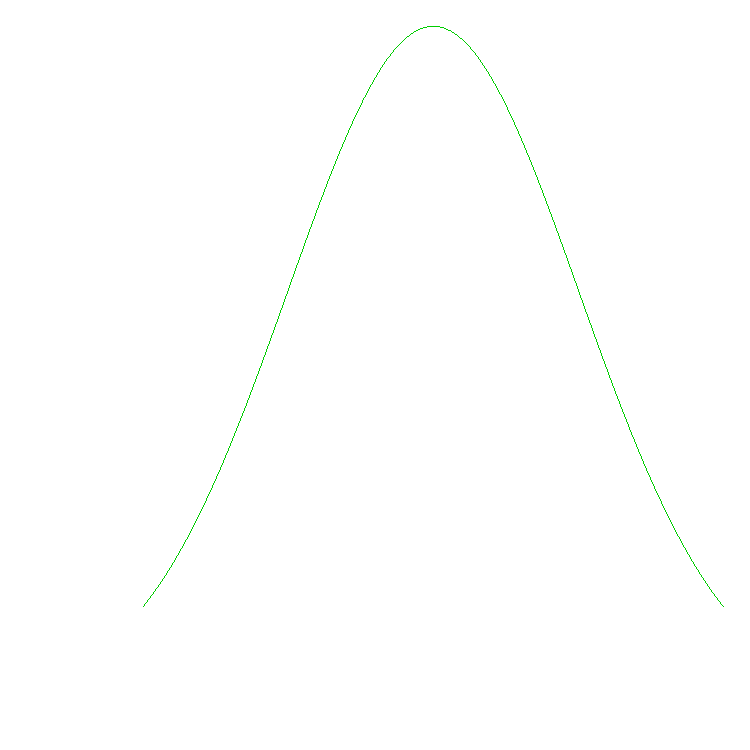
\includegraphics[width=\maxwidth]{figure/graphics-unnamed-chunk-146-1} 

}



\end{knitrout}
\caption{Grafico della distribuzione di Student a 10 gradi di libert\`a. }
\label{fig:graficostudent}
\end{center}
\end{figure}
Come nel caso della distribuzione normale se vogliamo una funzione diciamo \texttt{student}  tale che assegnato un valore di area $A$   fornisca l'ascissa $x=student(A)$  in modo che l'area tra - $x$ e $x$ sia esattamente pari ad $A$ dobbiamo scrivere la funzione
\begin{knitrout}
\definecolor{shadecolor}{rgb}{0.969, 0.969, 0.969}\color{fgcolor}\begin{kframe}
\begin{alltt}
\hlstd{student}\hlkwb{<-}\hlkwa{function} \hlstd{(}\hlkwc{A}\hlstd{,}\hlkwc{..}\hlstd{)} \hlkwd{qt} \hlstd{(}\hlnum{1}\hlopt{/}\hlnum{2} \hlopt{+} \hlstd{A}\hlopt{/}\hlnum{2}\hlstd{,..)}
\end{alltt}
\end{kframe}
\end{knitrout}
dove i puntini stanno per le variabili omesse o pi\`u esplicitamente
\begin{knitrout}
\definecolor{shadecolor}{rgb}{0.969, 0.969, 0.969}\color{fgcolor}\begin{kframe}
\begin{alltt}
\hlstd{student}\hlkwb{<-}\hlkwa{function} \hlstd{(}\hlkwc{A}\hlstd{,}\hlkwc{df}\hlstd{)} \hlkwd{qt} \hlstd{(}\hlnum{1}\hlopt{/}\hlnum{2} \hlopt{+} \hlstd{A}\hlopt{/}\hlnum{2}\hlstd{,df)}
\end{alltt}
\end{kframe}
\end{knitrout}
dove \texttt{df} sono i gradi di libert\`a. 
 \subsection
{Intervalli di confidenza e test di Student}
La funzione di
\textsf{R} che esegue il test di Student nelle sue diverse forme \`e  \texttt{t.test}.   Nella sua forma pi\`u semplice

\begin{knitrout}
\definecolor{shadecolor}{rgb}{0.969, 0.969, 0.969}\color{fgcolor}\begin{kframe}
\begin{alltt}
\hlstd{x}\hlkwb{=}\hlnum{1}\hlopt{:}\hlnum{20}\hlstd{;}  \hlkwd{t.test}\hlstd{(x)}
\end{alltt}
\begin{verbatim}
## 
## 	One Sample t-test
## 
## data:  x
## t = 7.9373, df = 19, p-value = 1.884e-07
## alternative hypothesis: true mean is not equal to 0
## 95 percent confidence interval:
##   7.731189 13.268811
## sample estimates:
## mean of x 
##      10.5
\end{verbatim}
\end{kframe}
\end{knitrout}
In assenza di ipotesi  \textsf{R} calcola il valore osservato del consuntivo $$T=\dfrac{M_N(X)-\mu}{S_X}\sqrt {N}$$
assumendo che sia $\mu=0$.
Possiamo anche eseguire specificare l'ipotesi sul valore di $\mu$:
\begin{knitrout}
\definecolor{shadecolor}{rgb}{0.969, 0.969, 0.969}\color{fgcolor}\begin{kframe}
\begin{alltt}
\hlkwd{t.test}\hlstd{(x,}\hlkwc{mu}\hlstd{=}\hlnum{7}\hlstd{)}
\end{alltt}
\begin{verbatim}
## 
## 	One Sample t-test
## 
## data:  x
## t = 2.6458, df = 19, p-value = 0.01595
## alternative hypothesis: true mean is not equal to 7
## 95 percent confidence interval:
##   7.731189 13.268811
## sample estimates:
## mean of x 
##      10.5
\end{verbatim}
\end{kframe}
\end{knitrout}
Possiamo infine specificare l'ipotesi alternativa. Per esempio se l'ipotesi alternativa \`e
\texttt{\virgolette less\virgolette}  il risultato del test cambia completamente.
\begin{knitrout}
\definecolor{shadecolor}{rgb}{0.969, 0.969, 0.969}\color{fgcolor}\begin{kframe}
\begin{alltt}
\hlkwd{t.test}\hlstd{(x,}\hlkwc{mu}\hlstd{=}\hlnum{7}\hlstd{,} \hlkwc{alternative}\hlstd{=}\hlstr{"less"}\hlstd{)}
\end{alltt}
\begin{verbatim}
## 
## 	One Sample t-test
## 
## data:  x
## t = 2.6458, df = 19, p-value = 0.992
## alternative hypothesis: true mean is less than 7
## 95 percent confidence interval:
##      -Inf 12.78743
## sample estimates:
## mean of x 
##      10.5
\end{verbatim}
\end{kframe}
\end{knitrout}

In pratica ci viene fornito come $p$-value il valore dell'area sottesa dalla distribuzione di Student da $-\infty$ al valore di $t$ se l'ipotesi alternativa \`e  \texttt{\virgolette less\virgolette} e il valore dell'area sottesa dalla distribuzione di Student dal valore di $t$ a $+\infty$ se l'ipotesi alternativa \`e     \texttt{\virgolette greater\virgolette}  \subsection{Test di Student per dati appaiati}
Il test di Student per dati appaiati non \`e altro che un test di Student sulla differenza di 2 liste di dati di ugual lunghezza. Consideriamo ad esempio il confronto di 2 tecniche di misura applicate agli stessi campioni
\begin{knitrout}
\definecolor{shadecolor}{rgb}{0.969, 0.969, 0.969}\color{fgcolor}\begin{kframe}
\begin{alltt}
\hlstd{x}\hlkwb{<-}\hlkwd{c}\hlstd{(}\hlnum{1.46}\hlstd{,}\hlnum{2.22}\hlstd{,}\hlnum{2.84}\hlstd{,}\hlnum{1.97}\hlstd{,}\hlnum{1.13}\hlstd{,}\hlnum{2.35}\hlstd{)}
\hlstd{y}\hlkwb{<-}\hlkwd{c}\hlstd{(}\hlnum{1.42}\hlstd{,}\hlnum{2.38}\hlstd{,}\hlnum{2.67}\hlstd{,}\hlnum{1.8}\hlstd{,}\hlnum{1.09}\hlstd{,}\hlnum{2.25}\hlstd{)}
\end{alltt}
\end{kframe}
\end{knitrout}

Possiamo calcolare la differenza \texttt{x-y} ed applicare il test di Student oppure ottenere lo stesso risultato specificando l'opzione \texttt{paired=TRUE}
\begin{knitrout}
\definecolor{shadecolor}{rgb}{0.969, 0.969, 0.969}\color{fgcolor}\begin{kframe}
\begin{alltt}
 \hlkwd{t.test}\hlstd{(x,y,}\hlkwc{paired}\hlstd{=}\hlnum{TRUE}\hlstd{)}
\end{alltt}
\begin{verbatim}
## 
## 	Paired t-test
## 
## data:  x and y
## t = 1.2, df = 5, p-value = 0.2839
## alternative hypothesis: true difference in means is not equal to 0
## 95 percent confidence interval:
##  -0.06852909  0.18852909
## sample estimates:
## mean of the differences 
##                    0.06
\end{verbatim}
\end{kframe}
\end{knitrout}

Il consuntivo   \texttt{t} cade entro la regione di accettazione del test.
\`E  possibile specificare il livello di fiducia da utilizzare per il test di Student come:

$$\texttt{conf.level}=\varia{numero}$$

Il comando completo di tutti i parametri  \`e quindi:
\begin{eqnarray*}
\texttt{t.test}(\varia{dati}_1,\varia{dati}_2,
\\
\texttt{paired=TRUE,conf.level}=\varia{valore})
\end{eqnarray*}
Ad esempio eseguiamo un $t$-test per dati appaiati, tra $x=(1,2,3,4)$ e $y=(3,2,4,5)$ con {\it confidence level} di 0.85. Scriveremo
\begin{knitrout}
\definecolor{shadecolor}{rgb}{0.969, 0.969, 0.969}\color{fgcolor}\begin{kframe}
\begin{alltt}
\hlkwd{t.test}\hlstd{(}\hlnum{1}\hlopt{:}\hlnum{4}\hlstd{,}\hlnum{5}\hlopt{:}\hlnum{2}\hlstd{,}\hlkwc{paired}\hlstd{=}\hlnum{TRUE}\hlstd{,}\hlkwc{conf.level}\hlstd{=}\hlnum{0.85}\hlstd{)}
\end{alltt}
\end{kframe}
\end{knitrout}
 Il consuntivo $t$ cade fuori dalla regione di accettazione proposta.


\subsection{t-test: caso ad egual varianza}

Si considerino i seguenti dati relativi alla misura di una grandezza fisica.


\[(
\color{red}{11.4},\color{blue}{23.7},\color{blue}{24.3},\color{red}{16.5},\color{blue}{28.5},
\color{blue}{26.6},\color{red}{21.1},\color{red}{29.9},\color{blue}{17.9},\color{red}{25.3},\color{blue}{14.2})\]


I colori rosso e blu si riferiscono all'utilizzo di due diversi strumenti di misura. Si noti che il numero di esperimenti in rosso (esperimenti 1,4, 7,8,10) non é uguale al numero di esperimenti in blu (esperimenti 2,3,5,6,9,11): non si tratta di misure ripetute sugli stessi campioni, ma di misure effettuate su campioni diversi.

Si dica, con fiducia al 95\% se esiste una differenza fra i due strumenti.
\begin{itemize}
\item I dati sono
\begin{knitrout}
\definecolor{shadecolor}{rgb}{0.969, 0.969, 0.969}\color{fgcolor}\begin{kframe}
\begin{verbatim}
## 11.4 16.5 21.1 29.9 25.3
## 23.7 24.3 28.5 26.6 17.9 14.2
\end{verbatim}
\end{kframe}
\end{knitrout}
\item Ipotesi di lavoro \[\mu_R= \mu_B\]
  \item Calcoliamo i valori dei parametri statistici per il campione rosso e per il campione blu.
\item Indicatori:
\[m_R=20.84\]
\[m_B=22.5333333\]
 \[s_R=7.2455504\]
\[s_B=5.4320039\]
\end{itemize}

Dobbiamo valutare il valore del consuntivo
\[ t_{ R, B} =\frac{ (M_R-M_B) -(\mu_R-\mu_B)}{\Sigma }\]
nell'ipotesi di lavoro 
\[\mu_R-\mu_B= 0\Leftrightarrow \mu_R=\mu_B\]

dove
\[
\begin{aligned}
\Sigma =& \sqrt{\dfrac{(n_R-1) S_R^2+(n_B-1) S_B^2 }{n_R+n_B-2}  \left(\frac{1}{n_R} +\frac{1}{n_B}\right)}\rightarrow  \\
&\sqrt{\dfrac{209.992+147.5333333 }{9}   \left(\frac{1}{5} +\frac{1}{6}\right)}= 
\sqrt{14.5658469} = 3.8165229
\end{aligned}
\] 

Il valore osservato di $t_{R,B}$ è

\[t_{ R,B} = \frac{m_R-m_B}{\Sigma}  =\ensuremath{-0.4436848} \]


La regione di accettazione \`e

\[[-t_{ 0.95, 9} , t_{0.95, 9} ] = [-2.262, 2.262]\]

Visto che il consuntivo  cade ampiamente in tale intervallo accettiamo l'ipotesi di lavoro.

con \rpr basta scrivere:
\begin{knitrout}
\definecolor{shadecolor}{rgb}{0.969, 0.969, 0.969}\color{fgcolor}\begin{kframe}
\begin{alltt}
\hlstd{R}\hlkwb{=}\hlkwd{c}\hlstd{(}\hlnum{11.4}\hlstd{,}\hlnum{16.5}\hlstd{,}\hlnum{21.1}\hlstd{,}\hlnum{29.9}\hlstd{,}\hlnum{25.3}\hlstd{)}
\hlstd{B}\hlkwb{=}\hlkwd{c}\hlstd{(}\hlnum{23.7}\hlstd{,}\hlnum{24.3}\hlstd{,}\hlnum{28.5}\hlstd{,}\hlnum{26.6}\hlstd{,} \hlnum{17.9}\hlstd{,}\hlnum{14.2}\hlstd{)}
\hlkwd{t.test}\hlstd{(R,B,}\hlkwc{var.equal}\hlstd{=T)}
\end{alltt}
\begin{verbatim}
## 
## 	Two Sample t-test
## 
## data:  R and B
## t = -0.44368, df = 9, p-value = 0.6677
## alternative hypothesis: true difference in means is not equal to 0
## 95 percent confidence interval:
##  -10.326908   6.940241
## sample estimates:
## mean of x mean of y 
##  20.84000  22.53333
\end{verbatim}
\end{kframe}
\end{knitrout}
Se non potessimo ipotizzare la provenienza dei due campioni da popolazioni con ugual varianza potremmo scrivere

\subsection{Caso generale (test di Welch)}

Qualora non si possa affermare l'eguaglianza delle varianze l'errore standard della differenza delle medie si può stimare come

\[ \Sigma= \sqrt{\frac{s_X^2}{n_X}+\frac{s_Y^2}{n_Y}}\]
\[ df =\dfrac
{ \left(\frac{s_X^2}{n_X}+\frac{s_Y^2}{n_Y}\right)^2}
{
\frac{(s_X^2/n_X)^2}{n_X-1}+
\frac{(s_Y^2/n_Y)^2}{n_Y-1}
}\]

Il consuntivo diviene

\[\frac{M_X-M_Y-(\mu_X-\mu_Y)}{\Sigma}  \]

e la regione di accettazione si calcola come

\[ [-t_{1-\epsilon,df},t_{1-\epsilon,df}]\]


\subsubsection{Esempio}
Con gli stessi dati di prima si ipotizzi $\mu_X=\mu_Y$ (fiducia al 95\%)

\[ X=(11.4, 16.5, 21.1, 29.9, 25.3)\quad Y=(23.7, 24.3, 28.5, 26.6, 17.9, 14.2)\]


\[ \Sigma= \sqrt{15.4173778}\]
e i gradi di libertà  
\[ df =\dfrac
{  (15.4173778)^2}
{
(110.2416002/4+
24.1845383/5)
}= \]
\[
  7.3368917
\]

Se si usa  \rpr basta scrivere

\begin{knitrout}
\definecolor{shadecolor}{rgb}{0.969, 0.969, 0.969}\color{fgcolor}\begin{kframe}
\begin{alltt}
\hlkwd{t.test}\hlstd{(X,Y)}
\end{alltt}
\begin{verbatim}
## 
## 	Welch Two Sample t-test
## 
## data:  X and Y
## t = -0.43126, df = 7.3369, p-value = 0.6787
## alternative hypothesis: true difference in means is not equal to 0
## 95 percent confidence interval:
##  -10.892293   7.505627
## sample estimates:
## mean of x mean of y 
##  20.84000  22.53333
\end{verbatim}
\end{kframe}
\end{knitrout}

\section{Test $\chi^2$  di indipendenza}

%code chunk
Consideriamo il seguente \emph{dataframe} che riporta le ambizioni di un gruppo di scolari americani
\begin{knitrout}
\definecolor{shadecolor}{rgb}{0.969, 0.969, 0.969}\color{fgcolor}\begin{kframe}
\begin{alltt}
\hlkwd{data}\hlstd{(bambini)}
\hlkwd{str}\hlstd{(bambini)}
\end{alltt}
\begin{verbatim}
## 'data.frame':	478 obs. of  11 variables:
##  $ Gender     : Factor w/ 2 levels "boy","girl": 1 1 2 2 2 2 2 2 2 2 ...
##  $ Grade      : int  5 5 5 5 5 5 5 5 5 5 ...
##  $ Age        : int  11 10 11 11 10 11 10 10 10 10 ...
##  $ Race       : Factor w/ 2 levels "Other","White": 2 2 2 2 2 2 2 2 2 2 ...
##  $ Urban.Rural: Factor w/ 3 levels "Rural","Suburban",..: 1 1 1 1 1 1 1 1 1 1 ...
##  $ School     : Factor w/ 9 levels "Brentwood Elementary",..: 4 4 4 4 4 4 4 4 4 4 ...
##  $ Goals      : Factor w/ 3 levels "Grades","Popular",..: 3 2 2 2 2 2 2 1 3 3 ...
##  $ Grades     : int  1 2 4 2 4 4 3 3 3 4 ...
##  $ Sports     : int  2 1 3 3 2 2 4 4 2 3 ...
##  $ Looks      : int  4 4 1 4 1 1 1 2 1 2 ...
##  $ Money      : int  3 3 2 1 3 3 2 1 4 1 ...
\end{verbatim}
\end{kframe}
\end{knitrout}

Nella tabella le colonne che ci interessano al momento sono quelle che riguardano il sesso, gli obiettivi (scelti tra successo scolastico, capacit\`a sportiva e popolarit\`a) e la provenienza (colonne 1, 5  e 7). Nelle colonne dalla 8 alla 11 sono messi in ordine di importanza per il conseguimento della popolarit\`a  voti, sport, aspetto esteriore e denaro.
%codechunk
 
Consideriamo per esempio le variabili provenienza e traguardi
\begin{knitrout}
\definecolor{shadecolor}{rgb}{0.969, 0.969, 0.969}\color{fgcolor}\begin{kframe}
\begin{alltt}
\hlstd{interessi2}\hlkwb{=}\hlstd{bambini[,}\hlkwd{c}\hlstd{(}\hlnum{5}\hlstd{,}\hlnum{7}\hlstd{)]}
\hlstd{tabella}\hlkwb{=}\hlkwd{table}\hlstd{(interessi2)}
\hlstd{tabella}
\end{alltt}
\begin{verbatim}
##            Goals
## Urban.Rural Grades Popular Sports
##    Rural        57      50     42
##    Suburban     87      42     22
##    Urban       103      49     26
\end{verbatim}
\end{kframe}
\end{knitrout}
 
Il test $\chi^2$  di indipendenza consente di  verificare se  due variabili sono indipendenti.
Se consideriamo le due variabili precedenti sesso e interessi.
\textsf{R}  dispone del comando \texttt{chisq.test},\index{\texttt{chisq.tst},test $\chi^2$}
dalla sintassi generale:$$\texttt{chisq.test}(\varia{tabella})$$
\begin{knitrout}
\definecolor{shadecolor}{rgb}{0.969, 0.969, 0.969}\color{fgcolor}\begin{kframe}
\begin{alltt}
\hlkwd{chisq.test}\hlstd{(tabella)}
\end{alltt}
\begin{verbatim}
## 
## 	Pearson's Chi-squared test
## 
## data:  tabella
## X-squared = 18.828, df = 4, p-value = 0.0008497
\end{verbatim}
\end{kframe}
\end{knitrout}
Nell'esempio degli studenti
%code chunk
\begin{knitrout}
\definecolor{shadecolor}{rgb}{0.969, 0.969, 0.969}\color{fgcolor}\begin{kframe}
\begin{alltt}
\hlkwd{data}\hlstd{(studenti)}
\hlkwd{str}\hlstd{(studenti)}
\end{alltt}
\begin{verbatim}
## 'data.frame':	96 obs. of  8 variables:
##  $ Sex : Factor w/ 2 levels "F","M": 2 2 2 1 2 1 2 2 1 1 ...
##  $ W   : num  86 53 64 61 64 51 78 55 59 52 ...
##  $ H   : num  1.9 1.76 1.74 1.64 1.8 1.68 1.78 1.68 1.68 1.67 ...
##  $ Eyes: Factor w/ 3 levels "azzurri","castani",..: 2 1 3 2 3 2 2 2 2 2 ...
##  $ Hair: Factor w/ 3 levels "biondi","castani",..: 3 2 2 2 2 2 2 3 2 2 ...
##  $ Sh  : int  48 42 41 39 42 38 42 40 38 39 ...
##  $ hM  : num  1.58 1.7 1.63 1.65 1.56 1.6 1.65 1.56 1.58 1.65 ...
##  $ hF  : num  1.82 1.6 1.8 1.78 1.75 1.75 1.75 1.7 1.83 1.7 ...
\end{verbatim}
\begin{alltt}
\hlstd{tabellaEH}\hlkwb{=}\hlkwd{table}\hlstd{(studenti}\hlopt{$}\hlstd{Eyes,studenti}\hlopt{$}\hlstd{Hair)}
\hlkwd{chisq.test}\hlstd{(tabellaEH)}
\end{alltt}


{\ttfamily\noindent\color{warningcolor}{\#\# Warning in chisq.test(tabellaEH): Chi-squared approximation may be incorrect}}\begin{verbatim}
## 
## 	Pearson's Chi-squared test
## 
## data:  tabellaEH
## X-squared = 5.9614, df = 4, p-value = 0.202
\end{verbatim}
\end{kframe}
\end{knitrout}
L'intervallo di accettazione dell'ipotesi (che ricordiamo \`e l'indipendenza) al 95\% di fiducia e 1 gradi di libert\`a \`e  $[0, 3.841]$, il consuntivo cade dentro, per cui l'ipotesi \`e accettata.
 
Se le celle in una tabella 2x2 contengono numeri bassi R utilizza la correzione di Yates. Se la si vuole eliminare  si utilizza il parametro  \texttt{correct=FALSE}.
Ad esempio scriveremo:
%code chunk
\begin{knitrout}
\definecolor{shadecolor}{rgb}{0.969, 0.969, 0.969}\color{fgcolor}\begin{kframe}
\begin{alltt}
\hlkwd{chisq.test}\hlstd{(}\hlkwd{matrix}\hlstd{(}\hlkwd{c}\hlstd{(}\hlnum{12}\hlstd{,}\hlnum{3}\hlstd{,}\hlnum{4}\hlstd{,}\hlnum{5}\hlstd{),}\hlkwc{nc}\hlstd{=}\hlnum{2}\hlstd{))}
\end{alltt}


{\ttfamily\noindent\color{warningcolor}{\#\# Warning in chisq.test(matrix(c(12, 3, 4, 5), nc = 2)): Chi-squared approximation may be incorrect}}\begin{verbatim}
## 
## 	Pearson's Chi-squared test with Yates'
## 	continuity correction
## 
## data:  matrix(c(12, 3, 4, 5), nc = 2)
## X-squared = 1.8, df = 1, p-value = 0.1797
\end{verbatim}
\begin{alltt}
\hlkwd{chisq.test}\hlstd{(}\hlkwd{matrix}\hlstd{(}\hlkwd{c}\hlstd{(}\hlnum{12}\hlstd{,}\hlnum{3}\hlstd{,}\hlnum{4}\hlstd{,}\hlnum{5}\hlstd{),}\hlkwc{nc}\hlstd{=}\hlnum{2}\hlstd{),}\hlkwc{correct}\hlstd{=F)}
\end{alltt}


{\ttfamily\noindent\color{warningcolor}{\#\# Warning in chisq.test(matrix(c(12, 3, 4, 5), nc = 2), correct = F): Chi-squared approximation may be incorrect}}\begin{verbatim}
## 
## 	Pearson's Chi-squared test
## 
## data:  matrix(c(12, 3, 4, 5), nc = 2)
## X-squared = 3.2, df = 1, p-value = 0.07364
\end{verbatim}
\end{kframe}
\end{knitrout}
\subsection{Test $\chi^2$  di adeguamento}
Consideriamo una variabile aleatoria discreta con frequenza assoluta delle uscite racchiuse in una lista \texttt{data}. Ci si pone il problema di stabilire se tali frequenze sono compatibili con le probabilit\`a (riportate nella lista $p$).
\begin{knitrout}
\definecolor{shadecolor}{rgb}{0.969, 0.969, 0.969}\color{fgcolor}\begin{kframe}
\begin{alltt}
\hlstd{data}\hlkwb{<-}\hlkwd{c}\hlstd{(}\hlnum{2}\hlstd{,}\hlnum{3}\hlstd{,}\hlnum{4}\hlstd{,}\hlnum{5}\hlstd{,}\hlnum{6}\hlstd{,}\hlnum{7}\hlstd{,}\hlnum{8}\hlstd{,}\hlnum{9}\hlstd{,}\hlnum{10}\hlstd{,}\hlnum{11}\hlstd{)}
\hlstd{prob}\hlkwb{<-}\hlkwd{c}\hlstd{(}\hlnum{5}\hlstd{,}\hlnum{20}\hlstd{,}\hlnum{5}\hlstd{,}\hlnum{10}\hlstd{,}\hlnum{5}\hlstd{,}\hlnum{15}\hlstd{,}\hlnum{5}\hlstd{,}\hlnum{10}\hlstd{,}\hlnum{10}\hlstd{,}\hlnum{15}\hlstd{)}
\hlkwd{sum}\hlstd{(prob)}
\hlkwd{chisq.test}\hlstd{(data,}\hlkwc{p}\hlstd{=prob,}\hlkwc{rescale.p}\hlstd{=}\hlnum{TRUE}\hlstd{)}
\end{alltt}
\end{kframe}
\end{knitrout}
Si \`e usata qui la scelta \texttt{rescale.p=TRUE} in quanto la somma delle  probabilit\`a non era 1.
L'uscita del test riporta il valore del consuntivo $\chi^2$ i gradi di libert\`a ed il valore $p$.

\section{Distribuzione Binomiale}
Il coefficiente binomiale \`e definito come
\begin{equation*} \texttt{choose}(\varia{n},\varia{m})={n \choose m}=\dfrac{n!}{m!\times (n-m)!}\end{equation*}
Ad esempio
\begin{knitrout}
\definecolor{shadecolor}{rgb}{0.969, 0.969, 0.969}\color{fgcolor}\begin{kframe}
\begin{alltt}
\hlkwd{choose}\hlstd{(}\hlnum{6}\hlstd{,}\hlnum{3}\hlstd{)}
\end{alltt}
\begin{verbatim}
## [1] 20
\end{verbatim}
\end{kframe}
\end{knitrout}
La distribuzione binomiale in \textsf{R} ha la sintassi $$\texttt{dbinom}(\varia{successi},\varia{prove},
\varia{probabilit\`a successo})$$ e fornisce la  probabilit\`a di ottenere nel corso di un certo numero di prove  il numero di successi indicato.\index{\texttt{dbinom}}
Ad esempio, nel lancio di un dado 10 volte, vogliamo determinare la  probabilit\`a che esca  \emph{esattamente} due volte il numero 4:
%codechunk
\begin{knitrout}
\definecolor{shadecolor}{rgb}{0.969, 0.969, 0.969}\color{fgcolor}\begin{kframe}
\begin{alltt}
\hlkwd{dbinom}\hlstd{(}\hlnum{2}\hlstd{,}\hlnum{10}\hlstd{,}\hlnum{1}\hlopt{/}\hlnum{6}\hlstd{)}
\end{alltt}
\begin{verbatim}
## [1] 0.29071
\end{verbatim}
\end{kframe}
\end{knitrout}

La  probabilit\`a \`e circa del 29\%.
\begin{comment}

\begin{shaded}
\begin{description}
 \item{}conta i caratteri del tuo nome
\item{} vettore che contenga il quadrato dei primi 8 numeri pari
\item{}vettore che contenga la radice cubica dei primi 10 numeri naturali.
\item{}inserire in una matrice le coordinate 2D dei punti di un pentagono. Plot dei punti, come punti, come linee e come linee tratteggiate. Pi\`u arduo: riempimento della superficie
\item{}derivata di $x^3+x^2+2x+1$, plot della funzione e plot della derivata come due pannelli distinti in un grafico unico. hint: par(mfrow)
\end{description}
\end{shaded}
\end{comment}
\begin{comment}

\section{Operatori condizionali e cicli}
with(rainforest, table(complete.cases(root), species))

Gli operatori condizionali valutano una condizione e in base alle risultanze assegnano valore ad una espressione

\begin{knitrout}
\definecolor{shadecolor}{rgb}{0.969, 0.969, 0.969}\color{fgcolor}\begin{kframe}
\begin{alltt}
\hlstd{b}\hlkwb{=}\hlnum{1}
\hlkwa{if} \hlstd{(b}\hlopt{==}\hlnum{1}\hlstd{) \{}\hlkwd{print} \hlstd{(}\hlstr{"b vale 1"}\hlstd{);b}\hlkwb{=}\hlstd{b}\hlopt{+}\hlnum{1}\hlstd{\}}  \hlkwa{else} \hlkwd{print}\hlstd{(b);}
\end{alltt}
\begin{verbatim}
## [1] "b vale 1"
\end{verbatim}
\end{kframe}
\end{knitrout}

Abbiamo poi i cicli \texttt{for} con la struttura
\begin{equation*}
\texttt{for} (i \texttt{it} \varia{sequenza}) \varia{esegui} B
\end{equation*}

\begin{knitrout}
\definecolor{shadecolor}{rgb}{0.969, 0.969, 0.969}\color{fgcolor}\begin{kframe}
\begin{alltt}
\hlkwa{for} \hlstd{(i} \hlkwa{in} \hlnum{1}\hlopt{:}\hlnum{10}\hlstd{)} \hlkwd{print}\hlstd{(i)}\hlcom{#Somma di interi}
\hlstd{somma}\hlkwb{<-}\hlnum{0}
\hlkwa{for} \hlstd{(i} \hlkwa{in}  \hlnum{1}\hlopt{:}\hlnum{10}\hlstd{) somma}\hlkwb{<-}\hlstd{somma}\hlopt{+}\hlstd{i;somma}
\hlcom{#o anche come funzione}
\hlstd{somma}\hlkwb{<-}\hlkwa{function}\hlstd{(}\hlkwc{n}\hlstd{)}
\hlstd{\{somma}\hlkwb{<-}\hlnum{0}
\hlkwa{for} \hlstd{(i} \hlkwa{in}  \hlnum{1}\hlopt{:}\hlstd{n) somma}\hlkwb{<-}\hlstd{somma}\hlopt{+}\hlstd{i;somma}
\hlkwd{return}\hlstd{(somma)\}}
\end{alltt}
\end{kframe}
\end{knitrout}


\section{Funzioni di pi\`u variabili}
Finora abbiamo considerato funzioni di singola variabile. Una generalizzazione estremamente naturale consiste nel considerare funzioni di due o pi\`u variabili. Diamo alcuni esempi
\begin{enumerate}
\item{}
Calcolare la lunghezza del segmento che congiunge  due punti nel piano (distanza euclidea). Possiamo procedere con  una funzione di 4 numeri (le 2 coordinate dei 2 punti)
\begin{knitrout}
\definecolor{shadecolor}{rgb}{0.969, 0.969, 0.969}\color{fgcolor}\begin{kframe}
\begin{alltt}
\hlstd{dist}\hlkwb{<-}\hlkwa{function}\hlstd{(}\hlkwc{x1}\hlstd{,}\hlkwc{y1}\hlstd{,}\hlkwc{x2}\hlstd{,}\hlkwc{y2}\hlstd{)}
\hlstd{\{dx}\hlkwb{<-}\hlstd{(x2}\hlopt{-}\hlstd{x1)}\hlopt{^}\hlnum{2}\hlstd{;dy}\hlkwb{<-}\hlstd{(y2}\hlopt{-}\hlstd{y1)}\hlopt{^}\hlnum{2}\hlstd{;}\hlkwd{return} \hlstd{(}\hlkwd{sqrt}\hlstd{(dx}\hlopt{+}\hlstd{dy))\}}
\hlkwd{dist}\hlstd{(}\hlnum{0}\hlstd{,}\hlnum{0}\hlstd{,}\hlnum{3}\hlstd{,}\hlnum{4}\hlstd{)}
\end{alltt}
\begin{verbatim}
## [1] 5
\end{verbatim}
\end{kframe}
\end{knitrout}
oppure possiamo generalizzare con una funzione che dipenda dai 2 vettori (e non direttamente dalle loro coordinate)
\begin{knitrout}
\definecolor{shadecolor}{rgb}{0.969, 0.969, 0.969}\color{fgcolor}\begin{kframe}
\begin{alltt}
\hlstd{dist}\hlkwb{<-}\hlkwa{function}\hlstd{(}\hlkwc{x}\hlstd{,}\hlkwc{y}\hlstd{)}
\hlstd{\{}\hlkwd{return} \hlstd{(}\hlkwd{sqrt}\hlstd{(}\hlkwd{sum}\hlstd{((x}\hlopt{-}\hlstd{y)}\hlopt{^}\hlnum{2}\hlstd{)))\}}
\end{alltt}
\end{kframe}
\end{knitrout}
\item{}: il massimo di due numeri
\begin{knitrout}
\definecolor{shadecolor}{rgb}{0.969, 0.969, 0.969}\color{fgcolor}\begin{kframe}
\begin{alltt}
\hlstd{massimo}\hlkwb{<-}\hlkwa{function}\hlstd{(}\hlkwc{a}\hlstd{,}\hlkwc{b}\hlstd{)}
\hlkwa{if} \hlstd{(a}\hlopt{>}\hlstd{b)} \hlkwd{return}\hlstd{(a)} \hlkwa{else} \hlkwd{return}\hlstd{(b)}
\end{alltt}
\end{kframe}
\end{knitrout}
Si noti che la condizione viene messa tra parentesi tonde.
\item{}: Il valore assoluto
\begin{knitrout}
\definecolor{shadecolor}{rgb}{0.969, 0.969, 0.969}\color{fgcolor}\begin{kframe}
\begin{alltt}
\hlstd{valoreassoluto}\hlkwb{<-}\hlkwa{function}\hlstd{(}\hlkwc{a}\hlstd{)} \hlkwa{if} \hlstd{(a}\hlopt{>}\hlnum{0}\hlstd{)} \hlkwd{return}\hlstd{(a)}  \hlkwa{else} \hlkwd{return}\hlstd{(}\hlopt{-}\hlstd{a)}
\end{alltt}
\end{kframe}
\end{knitrout}


\item{} Somma sino a $n$

\begin{knitrout}
\definecolor{shadecolor}{rgb}{0.969, 0.969, 0.969}\color{fgcolor}\begin{kframe}
\begin{alltt}
\hlstd{n}\hlkwb{=}\hlnum{0}\hlstd{;}\hlkwa{while} \hlstd{(}\hlkwd{somma}\hlstd{(n)}\hlopt{<}\hlnum{10000}\hlstd{)}
\hlstd{n}\hlkwb{=}\hlstd{n}\hlopt{+}\hlnum{1}
\hlstd{sommasinoa}\hlkwb{<-}\hlkwa{function}\hlstd{(}\hlkwc{b}\hlstd{) \{i}\hlkwb{<-}\hlnum{1}\hlstd{;somma}\hlkwb{<-}\hlstd{i;}\hlkwa{while} \hlstd{(somma}\hlopt{<=}\hlstd{b)}
\hlstd{\{i}\hlkwb{=}\hlstd{i}\hlopt{+}\hlnum{1}\hlstd{;somma}\hlkwb{=}\hlstd{somma}\hlopt{+}\hlstd{i\};} \hlkwd{return}\hlstd{(i)\}}
\end{alltt}
\end{kframe}
\end{knitrout}
\end{enumerate}


Generazione ricorsiva di successioni (successione di Fibonacci)
%code chunk
\begin{knitrout}
\definecolor{shadecolor}{rgb}{0.969, 0.969, 0.969}\color{fgcolor}\begin{kframe}
\begin{alltt}
\hlstd{fibonacci}\hlkwb{<-}\hlkwa{function}\hlstd{(}\hlkwc{n}\hlstd{)}
\hlstd{\{f}\hlkwb{=}\hlnum{0}\hlstd{;f[}\hlnum{1}\hlstd{]}\hlkwb{<-}\hlnum{1}\hlstd{;f[}\hlnum{2}\hlstd{]}\hlkwb{<-}\hlnum{1}\hlstd{;}\hlkwa{for} \hlstd{(i} \hlkwa{in} \hlnum{3}\hlopt{:}\hlstd{n) \{f[i]}\hlkwb{<-}\hlstd{f[i}\hlopt{-}\hlnum{1}\hlstd{]}\hlopt{+}\hlstd{f[i}\hlopt{-}\hlnum{2}\hlstd{]\};}\hlkwd{return}\hlstd{(f[n])\}}
\end{alltt}
\end{kframe}
\end{knitrout}

\section{R  Output su file}

\begin{knitrout}
\definecolor{shadecolor}{rgb}{0.969, 0.969, 0.969}\color{fgcolor}\begin{kframe}
\begin{alltt}
\hlkwd{cat}\hlstd{(}\hlstr{"TITLE extra line"}\hlstd{,} \hlstr{"2 4 5 7"}\hlstd{,} \hlstr{"11 13 17"}\hlstd{,} \hlkwc{file}\hlstd{=}\hlstr{"ex.data"}\hlstd{,} \hlkwc{sep}\hlstd{=}\hlstr{"\textbackslash{}n"}\hlstd{,}\hlkwc{append}\hlstd{=T)}
\hlkwd{cat}\hlstd{(}\hlstr{"TITLE extra line"}\hlstd{,} \hlstr{"2 4 5 7"}\hlstd{,} \hlstr{"11 13 17"}\hlstd{,} \hlkwc{sep}\hlstd{=}\hlstr{"\textbackslash{}n"}\hlstd{)}
\end{alltt}
\end{kframe}
\end{knitrout}
\begin{knitrout}
\definecolor{shadecolor}{rgb}{0.969, 0.969, 0.969}\color{fgcolor}\begin{kframe}
\begin{alltt}
\hlkwd{print}\hlstd{()}
\hlstd{read.delim}
 \hlstd{aggregate}
\end{alltt}
\end{kframe}
\end{knitrout}

\chapter{Statistica II parte}
%\section{Simulazioni e statistica Bayesiana}
Uno degli usi rilevanti a fini statistici dei computer  \`e la possibilit\`a di stimare attraverso simulazioni probabilit\`a difficili da calcolare teoricamente.
\begin{shaded}\begin{description}
\item{\bf Estrazioni da un'urna. }Supponiamo 2 palle siano estratte da un'urna contenente 6 palle rosse e 2 verdi.
Simuliamo due estrazioni e consideriamo gli eventi:
\begin{itemize}
\item{}$A$ = {la prima palla  \`e rossa}
\item{}$B$ = {la seconda palla \`e rossa}
\end{itemize}
Determinare le probabilit\`a
$P(A)$, $P(B)$,
$P(A\wedge B)$, $P(A \mid B)$,
$P(B \mid A)$.
Eseguire poi la simulazione 1000 volte e verificare che le stime frequentiste si avvicinano ai valori teorici. Si usi la funzione \texttt{replicates}.\index{\texttt{replicates}}
Gli ultimi due punti richiedono opportuni accorgimenti.
\item{\bf Simulazione del problema di  Monthy Hall.}
Il problema di Monthy Hall ricalca una trasmissione televisiva americana. Immaginate di avere tre porte chiuse dietro alle quali si nascondono 2 capre e un premio, una Ferrari per esempio. L'ospite deve scegliere una porta; effettuata tale scelta il presentatore (che conosce cosa si nasconde dietro alle 3 porte) apre una porta mostrando una capra e d\`a all'ospite la scelta se attenersi alla scelta originale o cambiare porta. Cosa fareste se foste voi l'ospite?
\end{description}
\end{shaded}
Come si pu\`o simulare il problema di Monthy Hall?
Iniziamo a disporre gli oggetti e a fare la nostra scelta
%code chunk
\begin{knitrout}
\definecolor{shadecolor}{rgb}{0.969, 0.969, 0.969}\color{fgcolor}\begin{kframe}
\begin{alltt}
\hlkwd{set.seed}\hlstd{(}\hlnum{12}\hlstd{)}
\hlstd{(}\hlkwd{sample}\hlstd{(}\hlkwd{c}\hlstd{(}\hlstr{"capra"}\hlstd{,}\hlstr{"capra"}\hlstd{,}\hlstr{"ferrari"}\hlstd{))}\hlkwb{->}\hlstd{posizione)}
\end{alltt}
\begin{verbatim}
## [1] "capra"   "capra"   "ferrari"
\end{verbatim}
\begin{alltt}
\hlstd{(scelta}\hlkwb{<-}\hlkwd{sample}\hlstd{(}\hlnum{1}\hlopt{:}\hlnum{3}\hlstd{,}\hlnum{1}\hlstd{))}
\end{alltt}
\begin{verbatim}
## [1] 1
\end{verbatim}
\end{kframe}
\end{knitrout}
A questo punto  il presentatore deve aprire una porta,
\begin{knitrout}
\definecolor{shadecolor}{rgb}{0.969, 0.969, 0.969}\color{fgcolor}\begin{kframe}
\begin{alltt}
\hlstd{(ammessa}\hlkwb{<-}\hlstd{(}\hlnum{1}\hlopt{:}\hlnum{3}\hlstd{)[}\hlopt{-}\hlkwd{unique}\hlstd{(}\hlkwd{c}\hlstd{(scelta,}\hlkwd{which}\hlstd{(posizione}\hlopt{==}\hlstr{"ferrari"}\hlstd{)))])}
\end{alltt}
\begin{verbatim}
## [1] 2
\end{verbatim}
\begin{alltt}
\hlkwa{if}\hlstd{(}\hlkwd{length}\hlstd{(ammessa)}\hlopt{==}\hlnum{1}\hlstd{)}
\hlstd{presentatore}\hlkwb{<-}\hlstd{ammessa} \hlkwa{else} \hlstd{presentatore}\hlkwb{=}\hlkwd{sample}\hlstd{(ammessa,}\hlnum{1}\hlstd{)}
\end{alltt}
\end{kframe}
\end{knitrout}
Ripetiamolo ora 1000 volte
\begin{knitrout}
\definecolor{shadecolor}{rgb}{0.969, 0.969, 0.969}\color{fgcolor}\begin{kframe}
\begin{alltt}
\hlkwd{replicate}\hlstd{(}\hlnum{1000}\hlstd{,\{}
\hlkwd{sample}\hlstd{(}\hlkwd{c}\hlstd{(}\hlstr{"capra"}\hlstd{,}\hlstr{"capra"}\hlstd{,}\hlstr{"ferrari"}\hlstd{))}\hlkwb{->}\hlstd{dietro;}
\hlstd{scelta}\hlkwb{=}\hlkwd{sample}\hlstd{(}\hlnum{1}\hlopt{:}\hlnum{3}\hlstd{,}\hlnum{1}\hlstd{);}
\hlstd{ammessi}\hlkwb{=}\hlstd{(}\hlnum{1}\hlopt{:}\hlnum{3}\hlstd{)[}\hlopt{-}\hlkwd{unique}\hlstd{(}\hlkwd{c}\hlstd{(scelta,}\hlkwd{which}\hlstd{(}
\hlstd{dietro}\hlopt{==}\hlstr{"ferrari"}\hlstd{)))];}
\hlkwa{if}\hlstd{(}\hlkwd{length}\hlstd{(ammessi)}\hlopt{==}\hlnum{1}\hlstd{) \{presentatore}\hlkwb{=}\hlstd{ammessi\}} \hlkwa{else} \hlstd{\{presentatore}\hlkwb{=}\hlkwd{sample}\hlstd{(ammessi,}\hlnum{1}\hlstd{)\};}
\hlkwd{c}\hlstd{(dietro[scelta],dietro[}\hlopt{-}\hlkwd{c}\hlstd{(scelta,presentatore)])\})}\hlkwb{->}\hlstd{risultato}
\hlkwd{table}\hlstd{(risultato[}\hlnum{1}\hlstd{,]);}\hlkwd{table}\hlstd{(risultato[}\hlnum{2}\hlstd{,]);}
\end{alltt}
\end{kframe}
\end{knitrout}

\section{Analisi della Varianza (ANOVA)}
L'analisi della varianza diviene estremamente semplice da eseguire con \textsf{R}  a patto di \emph{preparare} i dati in modo opportuno.
Consideriamo il seguente esempio tratto dal libro di Snedecor \cite{snedecor} in cui si considera l'assorbimento di grasso durante la cottura di 24 \emph{donuts}. Si esaminano 4 tipi di grasso di cottura 4 e la cottura di 6 \emph{donuts} per ciascun tipo. Inseriamo nella lista  $x$ il gruppo di appartenenza e nella lista $y$ le quantit\`a di grasso assorbito.
\begin{knitrout}
\definecolor{shadecolor}{rgb}{0.969, 0.969, 0.969}\color{fgcolor}\begin{kframe}
\begin{alltt}
\hlstd{x}\hlkwb{<-}\hlkwd{rep}\hlstd{(}\hlnum{1}\hlopt{:}\hlnum{4}\hlstd{,}\hlkwc{each}\hlstd{=}\hlnum{6}\hlstd{)}
\hlkwd{factor}\hlstd{(x)}\hlkwb{->}\hlstd{x}
\hlstd{x}\hlkwb{<-}\hlkwd{gl}\hlstd{(}\hlnum{4}\hlstd{,}\hlnum{6}\hlstd{);x}
\end{alltt}
\begin{verbatim}
##  [1] 1 1 1 1 1 1 2 2 2 2 2 2 3 3 3 3 3 3 4 4 4 4 4 4
## Levels: 1 2 3 4
\end{verbatim}
\begin{alltt}
\hlstd{y}\hlkwb{<-}\hlkwd{c}\hlstd{(}\hlnum{15}\hlstd{,}\hlnum{20}\hlstd{,}\hlnum{22}\hlstd{,}\hlnum{23}\hlstd{,}\hlnum{25}\hlstd{,}\hlnum{26}\hlstd{,}\hlnum{80}\hlstd{,}\hlnum{90}\hlstd{,}\hlnum{76}\hlstd{,}\hlnum{56}\hlstd{,}\hlnum{5}\hlstd{,}
\hlnum{43}\hlstd{,}\hlnum{23}\hlstd{,}\hlnum{45}\hlstd{,}\hlnum{67}\hlstd{,}\hlnum{89}\hlstd{,}\hlnum{87}\hlstd{,}\hlnum{65}\hlstd{,}\hlnum{43}\hlstd{,}\hlnum{23}\hlstd{,}\hlnum{45}\hlstd{,}\hlnum{10}\hlstd{,}\hlnum{11}\hlstd{,}\hlnum{23}\hlstd{)}
\hlstd{tabelladati}\hlkwb{=}\hlkwd{data.frame}\hlstd{(y,x)}
\hlstd{tabelladati}
\end{alltt}
\begin{verbatim}
##     y x
## 1  15 1
## 2  20 1
## 3  22 1
## 4  23 1
## 5  25 1
## 6  26 1
## 7  80 2
## 8  90 2
## 9  76 2
## 10 56 2
## 11  5 2
## 12 43 2
## 13 23 3
## 14 45 3
## 15 67 3
## 16 89 3
## 17 87 3
## 18 65 3
## 19 43 4
## 20 23 4
## 21 45 4
## 22 10 4
## 23 11 4
## 24 23 4
\end{verbatim}
\end{kframe}
\end{knitrout}
Il comando  \texttt{tapply} consente di applicare una funzione (in questo caso la media) alla lista  $y$ in base alla ripartizione indicata da $x$.
$$\texttt{tapply}(y,x,\texttt{mean})$$
In questo caso
\begin{knitrout}
\definecolor{shadecolor}{rgb}{0.969, 0.969, 0.969}\color{fgcolor}\begin{kframe}
\begin{alltt}
\hlkwd{tapply}\hlstd{(y,x,mean)}
\end{alltt}
\begin{verbatim}
##        1        2        3        4 
## 21.83333 58.33333 62.66667 25.83333
\end{verbatim}
\end{kframe}
\end{knitrout}
In modo simile all'uso del simbolo $\sim$ visto nei comandi per la regressione lineare il comando
$$\texttt{boxplot}(y\sim x,data=tabella)$$
consente il tracciamento di un \emph{boxplot} comparativo.
\begin{knitrout}
\definecolor{shadecolor}{rgb}{0.969, 0.969, 0.969}\color{fgcolor}\begin{kframe}
\begin{alltt}
\hlkwd{boxplot}\hlstd{(y}\hlopt{~}\hlstd{x,}\hlkwc{data}\hlstd{=tabelladati)}
\end{alltt}
\end{kframe}
\end{knitrout}
\begin{figure}[htbp]
\begin{center}
\begin{knitrout}
\definecolor{shadecolor}{rgb}{0.969, 0.969, 0.969}\color{fgcolor}\begin{kframe}


{\ttfamily\noindent\bfseries\color{errorcolor}{\#\# Error in getMetricsFromLatex(TeXMetrics, verbose = verbose): \\\#\# TeX was unable to calculate metrics for the following string\\\#\# or character:\\\#\# \\\#\# 	m\\\#\# \\\#\# Common reasons for failure include:\\\#\#\ \  * The string contains a character which is special to LaTeX unless\\\#\#\ \ \ \  escaped properly, such as \% or \$.\\\#\#\ \  * The string makes use of LaTeX commands provided by a package and\\\#\#\ \ \ \  the tikzDevice was not told to load the package.\\\#\# \\\#\# The contents of the LaTeX log of the aborted run have been printed above,\\\#\# it may contain additional details as to why the metric calculation failed.}}\end{kframe}

{\centering 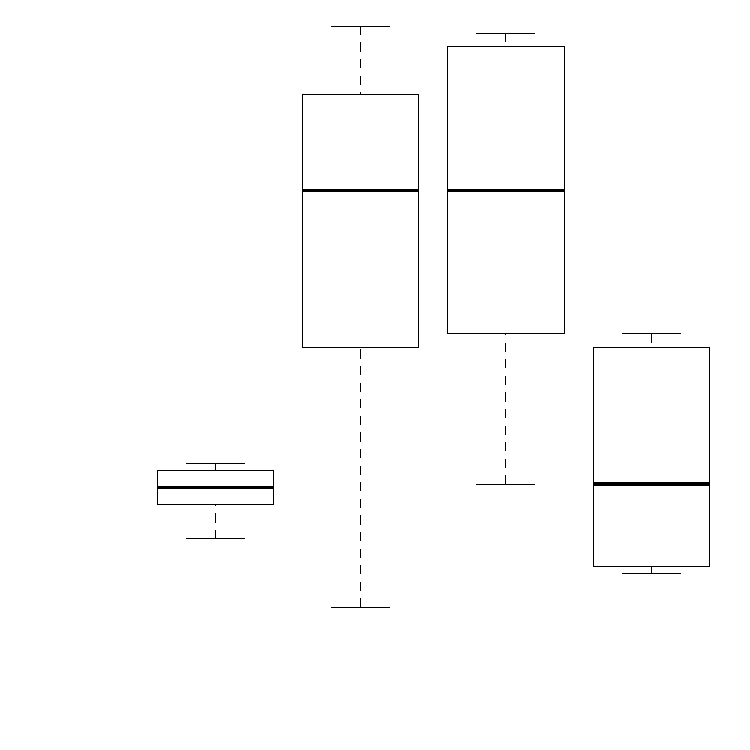
\includegraphics[width=\maxwidth]{figure/graphics-unnamed-chunk-184-1} 

}



\end{knitrout}
\caption{Boxplot comparativo di 4 tipi di grasso di cottura.}
\label{datiist}
\end{center}
\end{figure}
In modo analogo
\begin{knitrout}
\definecolor{shadecolor}{rgb}{0.969, 0.969, 0.969}\color{fgcolor}\begin{kframe}
\begin{alltt}
\hlkwd{anova}\hlstd{(}\hlkwd{lm}\hlstd{(y}\hlopt{~}\hlstd{x))}
\end{alltt}
\begin{verbatim}
## Analysis of Variance Table
## 
## Response: y
##           Df Sum Sq Mean Sq F value   Pr(>F)   
## x          3 8171.0 2723.67  5.8622 0.004833 **
## Residuals 20 9292.3  464.62                    
## ---
## Signif. codes:  
## 0 '***' 0.001 '**' 0.01 '*' 0.05 '.' 0.1 ' ' 1
\end{verbatim}
\end{kframe}
\end{knitrout}

fornisce il risultato dell'analisi della varianza.



\subsection{Test $\chi^2$  di indipendenza}

%code chunk
\begin{knitrout}
\definecolor{shadecolor}{rgb}{0.969, 0.969, 0.969}\color{fgcolor}\begin{kframe}
\begin{alltt}
\hlkwd{read.table}\hlstd{(}\hlstr{"../filedati/PopularKids.html"}\hlstd{,}\hlkwc{skip}\hlstd{=}\hlnum{39}\hlstd{,}\hlkwc{header}\hlstd{=T,}\hlkwc{nrow}\hlstd{=}\hlnum{478}\hlstd{,}\hlkwc{sep}\hlstd{=}\hlstr{"\textbackslash{}t"}\hlstd{)}\hlkwb{->}\hlstd{kidinterest}
\end{alltt}
\end{kframe}
\end{knitrout}
Il test $\chi^2$  di indipendenza consente di  verificare se  due variabili sono indipendenti.
Se consideriamo le due variabili precedenti sesso e interessi.
\textsf{R}  dispone del comando \texttt{chisq.test},\index{\texttt{chisq.tst},test $\chi^2$} dalla sintassi generale:$$\texttt{chisq.test}(\varia{tabella})$$

Nell'esempio
%code chunk
\begin{knitrout}
\definecolor{shadecolor}{rgb}{0.969, 0.969, 0.969}\color{fgcolor}\begin{kframe}
\begin{alltt}
\hlstd{tabellaEH}\hlkwb{=}\hlkwd{table}\hlstd{(studenti}\hlopt{$}\hlstd{Eyes,studenti}\hlopt{$}\hlstd{Hair)}
\hlkwd{chisq.test}\hlstd{(tabellaEH)}
\end{alltt}


{\ttfamily\noindent\color{warningcolor}{\#\# Warning in chisq.test(tabellaEH): Chi-squared approximation may be incorrect}}\begin{verbatim}
## 
## 	Pearson's Chi-squared test
## 
## data:  tabellaEH
## X-squared = 5.9614, df = 4, p-value = 0.202
\end{verbatim}
\end{kframe}
\end{knitrout}
L'intervallo di accettazione dell'ipotesi (che ricordiamo \`e l'indipendenza) al 95\% di fiducia e 1 gradi di libert\`a \`e  $[0, 3.841]$, il consuntivo cade dentro, per cui l'ipotesi \`e accettata.
Per eliminare la correzione di Pearson si utilizza il parametro  \texttt{correct=FALSE}.
Ad esempio scriveremo:
%code chunk
\begin{knitrout}
\definecolor{shadecolor}{rgb}{0.969, 0.969, 0.969}\color{fgcolor}\begin{kframe}
\begin{alltt}
\hlkwd{chisq.test}\hlstd{(tabellaEH,}\hlkwc{correct}\hlstd{=}\hlnum{FALSE}\hlstd{)}
\end{alltt}
\end{kframe}
\end{knitrout}

\subsection{Test $\chi^2$  di adeguamento}
Consideriamo una variabile aleatoria discreta con frequenza assoluta delle uscite racchiuse in una lista \texttt{data}. Ci si pone il problema di stabilire se tali frequenze sono compatibili con le probabilit\`a (riportate nella lista $p$).
\begin{knitrout}
\definecolor{shadecolor}{rgb}{0.969, 0.969, 0.969}\color{fgcolor}\begin{kframe}
\begin{alltt}
\hlstd{data}\hlkwb{<-}\hlkwd{c}\hlstd{(}\hlnum{2}\hlstd{,}\hlnum{3}\hlstd{,}\hlnum{4}\hlstd{,}\hlnum{5}\hlstd{,}\hlnum{6}\hlstd{,}\hlnum{7}\hlstd{,}\hlnum{8}\hlstd{,}\hlnum{9}\hlstd{,}\hlnum{10}\hlstd{,}\hlnum{11}\hlstd{)}
\hlstd{prob}\hlkwb{<-}\hlkwd{c}\hlstd{(}\hlnum{5}\hlstd{,}\hlnum{20}\hlstd{,}\hlnum{5}\hlstd{,}\hlnum{10}\hlstd{,}\hlnum{5}\hlstd{,}\hlnum{15}\hlstd{,}\hlnum{5}\hlstd{,}\hlnum{10}\hlstd{,}\hlnum{10}\hlstd{,}\hlnum{15}\hlstd{)}
\hlkwd{sum}\hlstd{(prob)}
\hlkwd{chisq.test}\hlstd{(data,}\hlkwc{p}\hlstd{=prob,}\hlkwc{rescale.p}\hlstd{=}\hlnum{TRUE}\hlstd{)}
\end{alltt}
\end{kframe}
\end{knitrout}
Si \`e usata qui la scelta \texttt{rescale.p=TRUE} in quanto la somma delle  probabilit\`a non era 1.
L'uscita del test riporta il valore del consuntivo $\chi^2$ i gradi di libert\`a ed il valore $p$.

\section{Distribuzione Binomiale}
Il coefficiente binomiale \`e definito come
\begin{equation*} \texttt{choose}(\varia{n},\varia{m})={n \choose m}=\dfrac{n!}{m!\times (n-m)!}\end{equation*}
Ad esempio
\begin{knitrout}
\definecolor{shadecolor}{rgb}{0.969, 0.969, 0.969}\color{fgcolor}\begin{kframe}
\begin{alltt}
\hlkwd{choose}\hlstd{(}\hlnum{6}\hlstd{,}\hlnum{3}\hlstd{)}
\end{alltt}
\begin{verbatim}
## [1] 20
\end{verbatim}
\end{kframe}
\end{knitrout}
La distribuzione binomiale in \textsf{R} ha la sintassi $$\texttt{dbinom}(\varia{successi},\varia{prove},
\varia{probabilit\`a successo})$$ e fornisce la  probabilit\`a di ottenere nel corso di un certo numero di prove  il numero di successi indicato.\index{\texttt{dbinom}}
Ad esempio, nel lancio di un dado 10 volte, vogliamo determinare la  probabilit\`a che esca  \emph{esattamente} due volte il numero 4:
%codechunk
\begin{knitrout}
\definecolor{shadecolor}{rgb}{0.969, 0.969, 0.969}\color{fgcolor}\begin{kframe}
\begin{alltt}
\hlkwd{dbinom}\hlstd{(}\hlnum{2}\hlstd{,}\hlnum{10}\hlstd{,}\hlnum{1}\hlopt{/}\hlnum{6}\hlstd{)}
\end{alltt}
\begin{verbatim}
## [1] 0.29071
\end{verbatim}
\end{kframe}
\end{knitrout}

La  probabilit\`a \`e circa del 29\%.


\section{Distribuzione di Fisher}

La distribuzione di Fisher \`e indicata in \textsf{R} con la lettera \texttt{f}. Per tracciare il grafico della densit\`a con gradi di libert\`a $\nu_1$ e $\nu_2$ basta scrivere
\begin{knitrout}
\definecolor{shadecolor}{rgb}{0.969, 0.969, 0.969}\color{fgcolor}\begin{kframe}
\begin{alltt}
\hlkwd{curve}\hlstd{(}\hlkwd{df}\hlstd{(x,}\hlnum{3}\hlstd{,}\hlnum{10}\hlstd{),}\hlnum{0}\hlstd{,}\hlnum{5}\hlstd{)}
\end{alltt}


{\ttfamily\noindent\bfseries\color{errorcolor}{\#\# Error in getMetricsFromLatex(TeXMetrics, verbose = verbose): \\\#\# TeX was unable to calculate metrics for the following string\\\#\# or character:\\\#\# \\\#\# 	m\\\#\# \\\#\# Common reasons for failure include:\\\#\#\ \  * The string contains a character which is special to LaTeX unless\\\#\#\ \ \ \  escaped properly, such as \% or \$.\\\#\#\ \  * The string makes use of LaTeX commands provided by a package and\\\#\#\ \ \ \  the tikzDevice was not told to load the package.\\\#\# \\\#\# The contents of the LaTeX log of the aborted run have been printed above,\\\#\# it may contain additional details as to why the metric calculation failed.}}\end{kframe}

{\centering 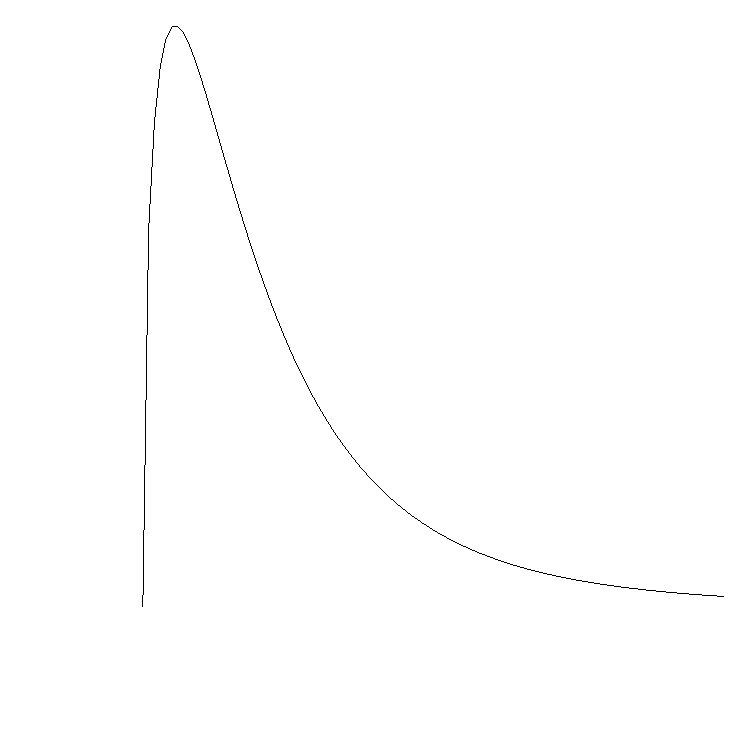
\includegraphics[width=\maxwidth]{figure/graphics-unnamed-chunk-192-1} 

}



\end{knitrout}
ottenendo il grafico
\begin{figure}[htbp]
\begin{center}
\begin{knitrout}
\definecolor{shadecolor}{rgb}{0.969, 0.969, 0.969}\color{fgcolor}\begin{kframe}
\begin{alltt}
\hlkwd{curve}\hlstd{(}\hlkwd{df}\hlstd{(x,}\hlnum{3}\hlstd{,}\hlnum{10}\hlstd{),}\hlnum{0}\hlstd{,}\hlnum{5}\hlstd{)}
\end{alltt}


{\ttfamily\noindent\bfseries\color{errorcolor}{\#\# Error in getMetricsFromLatex(TeXMetrics, verbose = verbose): \\\#\# TeX was unable to calculate metrics for the following string\\\#\# or character:\\\#\# \\\#\# 	m\\\#\# \\\#\# Common reasons for failure include:\\\#\#\ \  * The string contains a character which is special to LaTeX unless\\\#\#\ \ \ \  escaped properly, such as \% or \$.\\\#\#\ \  * The string makes use of LaTeX commands provided by a package and\\\#\#\ \ \ \  the tikzDevice was not told to load the package.\\\#\# \\\#\# The contents of the LaTeX log of the aborted run have been printed above,\\\#\# it may contain additional details as to why the metric calculation failed.}}\end{kframe}

{\centering 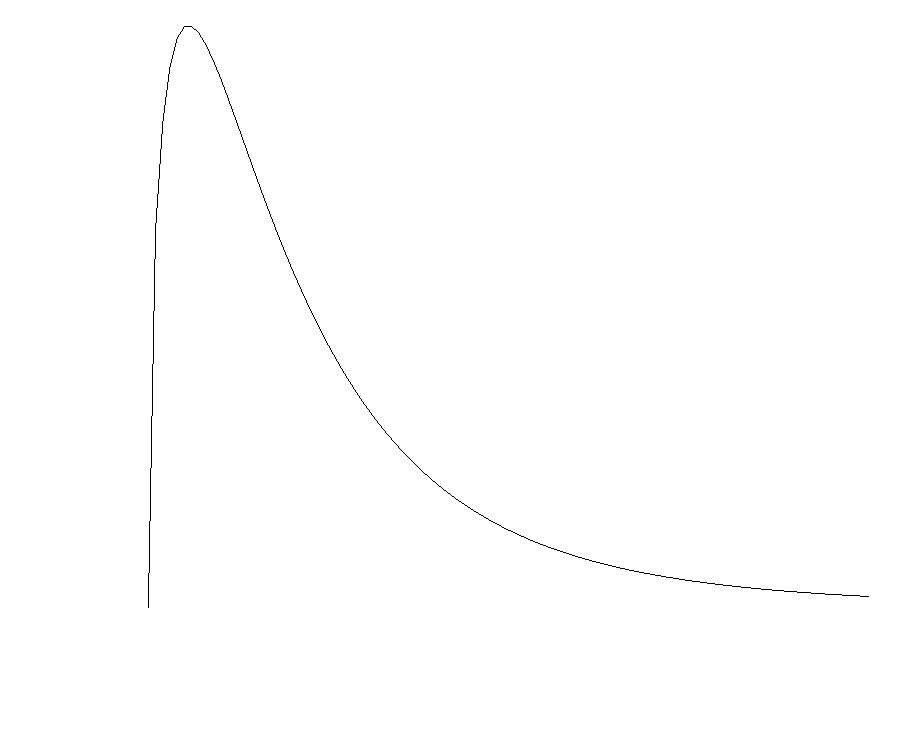
\includegraphics[width=\maxwidth]{figure/graphics-unnamed-chunk-193-1} 

}



\end{knitrout}
\caption{Distribuzione di Fisher.}
\label{fig:fisher}
\end{center}
\end{figure}.

Dobbiamo solo definire $x$, $df1$ e $df2$, gradi di libert\`a per poi applicare \texttt{df},\texttt{qf}, \texttt{rf} come visto per le distribuzioni precedenti.
Per esempio per ottenere il valore della funzione inversa  per $x=0.9$ e $df1=3$ e $df2=4$ scriveremo:
\begin{knitrout}
\definecolor{shadecolor}{rgb}{0.969, 0.969, 0.969}\color{fgcolor}\begin{kframe}
\begin{alltt}
\hlkwd{qf}\hlstd{(}\hlnum{0.9}\hlstd{,}\hlnum{3}\hlstd{,}\hlnum{4}\hlstd{)}
\end{alltt}
\begin{verbatim}
## [1] 4.19086
\end{verbatim}
\end{kframe}
\end{knitrout}


\section{Tabelle di contingenza}

Il comando
$\texttt{table}$ applicato ad un lista contenente valori di una singola variabile nominale conta le frequenze di ciascuna livello, se applicato ad un \emph{dataframe} di $n$  variabili conta le occorrenze di  ciascuna combinazione di livelli possibile ($2^n$ se le variabili sono dicotomiche). Per esempio se consideriamo il \emph{dataframe}  \texttt{studenti}  possiamo creare una tabella dei colori degli occhi e dei capelli
%code chunk
\begin{knitrout}
\definecolor{shadecolor}{rgb}{0.969, 0.969, 0.969}\color{fgcolor}\begin{kframe}
\begin{alltt}
\hlstd{tabellaEH}\hlkwb{=}\hlkwd{table}\hlstd{(studenti}\hlopt{$}\hlstd{Eyes,studenti}\hlopt{$}\hlstd{Hair)}
\end{alltt}
\end{kframe}
\end{knitrout}






\section{Farmacocinetica e modelli non lineari}

Dopo la somministrazione, un farmaco viene distribuito alle regioni del corpo accessibili.
Se consideriamo questo evento istantaneo, il corpo pu\`o qui essere considerato un contenitore omogeneo del farmaco, e la cinetica di diffusione pu\`o essere modellata con un modello a singolo compartimento aperto.
Quest'ultimo termine significa che il contenuto del compartimento non \`e confinato nel compartimento.
Se invece la diffusione non \`e istantanea e il contenuto arriva al siero secondo un modello di decrescita malthusiana,  il sistema  pu\`o essere modellato come un sistema a due compartimenti aperti.

Il dataset \texttt{Theoph} contiene 11 misure di concentrazione (a diversa tempistica) per ciascuno dei 12 soggetti sottoposti a somministrazione orale di teofillina.
\begin{knitrout}
\definecolor{shadecolor}{rgb}{0.969, 0.969, 0.969}\color{fgcolor}\begin{kframe}
\begin{alltt}
\hlkwd{head}\hlstd{(Theoph)}
\end{alltt}
\begin{verbatim}
##   Subject   Wt Dose Time  conc
## 1       1 79.6 4.02 0.00  0.74
## 2       1 79.6 4.02 0.25  2.84
## 3       1 79.6 4.02 0.57  6.57
## 4       1 79.6 4.02 1.12 10.50
## 5       1 79.6 4.02 2.02  9.66
## 6       1 79.6 4.02 3.82  8.58
\end{verbatim}
\end{kframe}
\end{knitrout}
Diamo una prima occhiata ai dati con il comando \texttt{coplot}, ovvero {\it conditioning plot}.  Il comando richiede un modello/formula, del tipo $(x y|a)$, che significa $x$ versus $y$ dato $a$ (ecco perch? conditioning). Se le variabili rispetto alle quali riportare il grafico sono pi\`u di una, basta aggiungere tra esse un segno $+$.
\begin{knitrout}
\definecolor{shadecolor}{rgb}{0.969, 0.969, 0.969}\color{fgcolor}\begin{kframe}
\begin{alltt}
\hlkwd{require}\hlstd{(graphics)}
\hlkwd{coplot}\hlstd{(conc} \hlopt{~} \hlstd{Time} \hlopt{|} \hlstd{Subject,} \hlkwc{data} \hlstd{= Theoph,} \hlkwc{show.given} \hlstd{=} \hlnum{FALSE}\hlstd{)}
\end{alltt}


{\ttfamily\noindent\bfseries\color{errorcolor}{\#\# Error in getMetricsFromLatex(TeXMetrics, verbose = verbose): \\\#\# TeX was unable to calculate metrics for the following string\\\#\# or character:\\\#\# \\\#\# 	m\\\#\# \\\#\# Common reasons for failure include:\\\#\#\ \  * The string contains a character which is special to LaTeX unless\\\#\#\ \ \ \  escaped properly, such as \% or \$.\\\#\#\ \  * The string makes use of LaTeX commands provided by a package and\\\#\#\ \ \ \  the tikzDevice was not told to load the package.\\\#\# \\\#\# The contents of the LaTeX log of the aborted run have been printed above,\\\#\# it may contain additional details as to why the metric calculation failed.}}\end{kframe}

{\centering 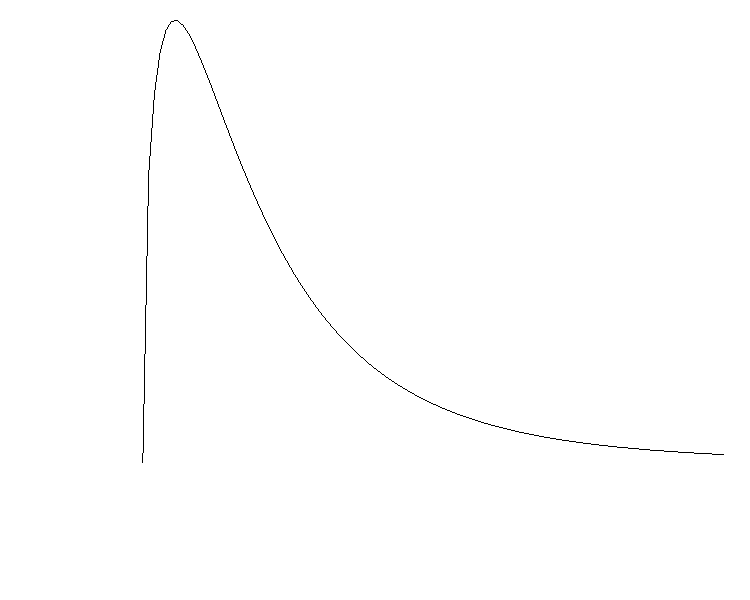
\includegraphics[width=\maxwidth]{figure/graphics-unnamed-chunk-198-1} 

}



\end{knitrout}

Selezioniamo ora il paziente 4, lo possiamo fare note le righe che esso occupa nel dataframe oppure selezionando per un preciso valore della variabile Subject.

\begin{knitrout}
\definecolor{shadecolor}{rgb}{0.969, 0.969, 0.969}\color{fgcolor}\begin{kframe}
\begin{alltt}
\hlstd{Theoph.4} \hlkwb{<-} \hlkwd{subset}\hlstd{(Theoph, Subject} \hlopt{==} \hlnum{4}\hlstd{)}
\end{alltt}
\end{kframe}
\end{knitrout}
\subsection{Regressione non lineare}
In statistica, una regressione non lineare \`e una forma di regressione in cui i dati osservati sono modellati da una funzione che non \`e una combinazione lineare dei parametri e che dipende da una o pi\`u  variabili indipendenti.

Il comando \texttt{nls} determina le stime dei parametri di un modello non lineare con il metodo dei minimi quadrati (ponderati).
Se consideriamo un modello a 2 compartimenti aperti del primo ordine descritto da sistema di equazioni differenziali
\begin{equation}\begin{cases}
x'(t)&= -k_a x(t)\\
y'(t)&= k_a x(t)-k_e y(t)
\end{cases}
\end{equation}
troviamo la soluzione
\begin{equation}
\begin{cases}
x(t)=&x_0 e^{-k_a t}\\
y(t) =&x_0 k_a  \frac{e^{-k_e t} - e^{-k_a t}}{k_a-k_e}
\end{cases}
 \end{equation}
In particolare la funzione \texttt{SSfol} in \textsf{R} consente di descrivere una cinetica del primo ordine per il modello a proposto. Essa infatti restituisce i logaritmi dei parametri di eliminazione, assorbimento e  \emph{clearance} (\texttt{lKe, lKa, lCl}).
L'uso \`e il seguente
\begin{equation*}\texttt{SSfol(Dose, input, lKe, lKa, lCl})
\end{equation*}
dove \texttt{Dose}  rappresenta la dose iniziale,  \texttt{input} \`e un vettore numerico con il quale valutiamo il modello. \texttt{lKe} \`e un parametro numerico che rappresenta il logaritmo naturale della costante velocit\`a di eliminazione. \texttt{lKa} \`e un parametro numerico che rappresenta il logaritmo naturale della costante velocit\`a di assorbimento mentre  \texttt{lCl} \`e un parametro numerico che rappresenta il logaritmo naturale  della \emph{clearance}.
Proviamo ad utilizzare il comando \texttt{SSfol}, e inseriamo il risultato della regressione nella variabile \texttt{fm1} (modello 1).
%code chunk
\begin{knitrout}
\definecolor{shadecolor}{rgb}{0.969, 0.969, 0.969}\color{fgcolor}\begin{kframe}
\begin{alltt}
\hlstd{fm1} \hlkwb{<-} \hlkwd{nls}\hlstd{(conc} \hlopt{~} \hlkwd{SSfol}\hlstd{(Dose, Time, lKe, lKa, lCl),} \hlkwc{data} \hlstd{= Theoph.4)}
\end{alltt}
\end{kframe}
\end{knitrout}
Osserviamo \texttt{fm1},  con il comando \texttt{summary}
\begin{knitrout}
\definecolor{shadecolor}{rgb}{0.969, 0.969, 0.969}\color{fgcolor}\begin{kframe}
\begin{alltt}
\hlkwd{summary}\hlstd{(fm1)}
\end{alltt}
\begin{verbatim}
## 
## Formula: conc ~ SSfol(Dose, Time, lKe, lKa, lCl)
## 
## Parameters:
##     Estimate Std. Error t value Pr(>|t|)    
## lKe  -2.4365     0.2257 -10.797 4.77e-06 ***
## lKa   0.1583     0.2297   0.689     0.51    
## lCl  -3.2861     0.1448 -22.695 1.51e-08 ***
## ---
## Signif. codes:  
## 0 '***' 0.001 '**' 0.01 '*' 0.05 '.' 0.1 ' ' 1
## 
## Residual standard error: 0.8465 on 8 degrees of freedom
## 
## Number of iterations to convergence: 7 
## Achieved convergence tolerance: 2.969e-06
\end{verbatim}
\end{kframe}
\end{knitrout}

Ora riportiamo il grafico delle osservazioni per il soggetto 4 su un grafico singolo:

\begin{knitrout}
\definecolor{shadecolor}{rgb}{0.969, 0.969, 0.969}\color{fgcolor}\begin{kframe}
\begin{alltt}
\hlkwd{options}\hlstd{(}\hlkwc{width}\hlstd{=}\hlnum{40}\hlstd{)}
\hlkwd{plot}\hlstd{(conc} \hlopt{~} \hlstd{Time,} \hlkwc{data} \hlstd{= Theoph.4,}
\hlkwc{xlab} \hlstd{=} \hlstr{"tempo dalla somministazione (ore)"}\hlstd{,}
 \hlkwc{ylab} \hlstd{=} \hlstr{"Concentrazione di Teofillina(mg/L)"}\hlstd{,}
\hlkwc{main} \hlstd{=} \hlstr{"Concentrazioni osservate e modello"}\hlstd{,} \hlkwc{sub} \hlstd{=} \hlstr{"Soggetto 4"}\hlstd{,}
\hlkwc{las} \hlstd{=} \hlnum{1}\hlstd{,} \hlkwc{col} \hlstd{=} \hlnum{4}\hlstd{)}
\end{alltt}


{\ttfamily\noindent\bfseries\color{errorcolor}{\#\# Error in getMetricsFromLatex(TeXMetrics, verbose = verbose): \\\#\# TeX was unable to calculate metrics for the following string\\\#\# or character:\\\#\# \\\#\# 	m\\\#\# \\\#\# Common reasons for failure include:\\\#\#\ \  * The string contains a character which is special to LaTeX unless\\\#\#\ \ \ \  escaped properly, such as \% or \$.\\\#\#\ \  * The string makes use of LaTeX commands provided by a package and\\\#\#\ \ \ \  the tikzDevice was not told to load the package.\\\#\# \\\#\# The contents of the LaTeX log of the aborted run have been printed above,\\\#\# it may contain additional details as to why the metric calculation failed.}}\end{kframe}

{\centering 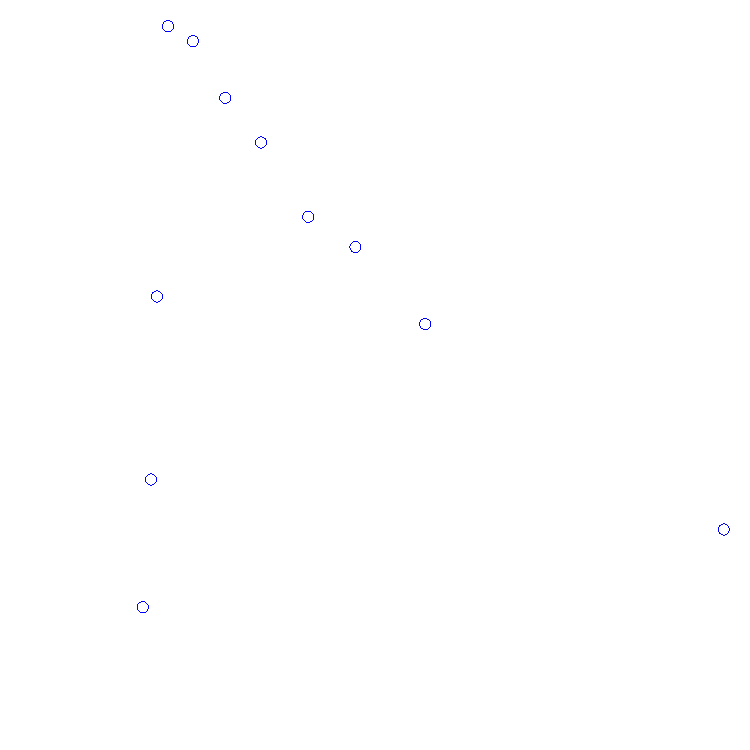
\includegraphics[width=\maxwidth]{figure/graphics-unnamed-chunk-202-1} 

}



\end{knitrout}

Si pu\`o ora sovrapporre la curva ottenuta con il modello al grafico attuale.
Per prima cosa definiamo i possibili valori di $x$.

\begin{knitrout}
\definecolor{shadecolor}{rgb}{0.969, 0.969, 0.969}\color{fgcolor}\begin{kframe}
\begin{alltt}
\hlstd{xvals} \hlkwb{<-} \hlkwd{seq}\hlstd{(}\hlnum{0}\hlstd{,} \hlkwd{par}\hlstd{(}\hlstr{"usr"}\hlstd{)[}\hlnum{2}\hlstd{],} \hlkwc{length.out} \hlstd{=} \hlnum{55}\hlstd{)}
\end{alltt}
\end{kframe}
\end{knitrout}

dove \texttt{par(usr)}  \`e un ottimo modo per conoscere l'estensione di una delle dimensioni della finestra grafica. A tali valori di $x$ vengono associati i corrispettivi valori $y$ della curva, ottenuti con il comando \texttt{predict}, che utilizza diversi metodi predittivi noti i valori delle costanti del modello ed i valori di $x$. In questo caso il tempo (la nostra $x$)  \`e  uguale ai valori \texttt{xvars} appena calcolati.

\begin{knitrout}
\definecolor{shadecolor}{rgb}{0.969, 0.969, 0.969}\color{fgcolor}\begin{kframe}
\begin{alltt}
\hlkwd{plot}\hlstd{(conc} \hlopt{~} \hlstd{Time,} \hlkwc{data} \hlstd{= Theoph.4,}
\hlkwc{xlab} \hlstd{=} \hlstr{"tempo dalla somministazione (ore)"}\hlstd{,}
\hlkwc{ylab} \hlstd{=} \hlstr{"Concentrazione di Teofillina(mg/L)"}\hlstd{,}
\hlkwc{main} \hlstd{=} \hlstr{"Concentrazioni osservate e modello"}\hlstd{,} \hlkwc{sub} \hlstd{=} \hlstr{"Soggetto 4"}\hlstd{,}
\hlkwc{las} \hlstd{=} \hlnum{1}\hlstd{,} \hlkwc{col} \hlstd{=} \hlnum{4}\hlstd{)}
\end{alltt}


{\ttfamily\noindent\bfseries\color{errorcolor}{\#\# Error in getMetricsFromLatex(TeXMetrics, verbose = verbose): \\\#\# TeX was unable to calculate metrics for the following string\\\#\# or character:\\\#\# \\\#\# 	m\\\#\# \\\#\# Common reasons for failure include:\\\#\#\ \  * The string contains a character which is special to LaTeX unless\\\#\#\ \ \ \  escaped properly, such as \% or \$.\\\#\#\ \  * The string makes use of LaTeX commands provided by a package and\\\#\#\ \ \ \  the tikzDevice was not told to load the package.\\\#\# \\\#\# The contents of the LaTeX log of the aborted run have been printed above,\\\#\# it may contain additional details as to why the metric calculation failed.}}\begin{alltt}
\hlkwd{lines}\hlstd{(xvals,} \hlkwd{predict}\hlstd{(fm1,} \hlkwc{newdata} \hlstd{=} \hlkwd{list}\hlstd{(}\hlkwc{Time} \hlstd{= xvals)),} \hlkwc{col} \hlstd{=} \hlnum{4}\hlstd{)}
\end{alltt}
\end{kframe}

{\centering 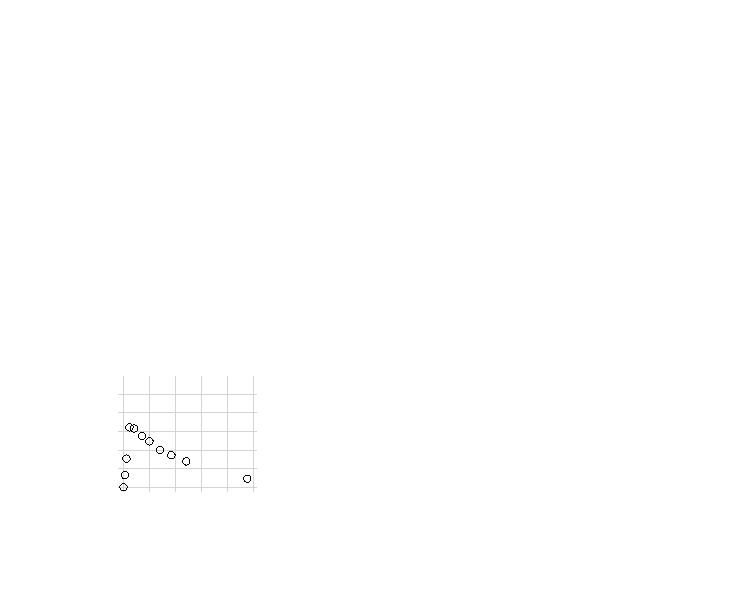
\includegraphics[width=\maxwidth]{figure/graphics-unnamed-chunk-204-1} 

}



\end{knitrout}
\chpater{Varie}
\subsubsection{La funzione \texttt{apply}}
Quando abbiamo una struttura di dati a pi\`u dimensioni ad esempio un \emph{array}
\begin{knitrout}
\definecolor{shadecolor}{rgb}{0.969, 0.969, 0.969}\color{fgcolor}\begin{kframe}
\begin{alltt}
\hlkwd{array}\hlstd{(}\hlnum{1}\hlopt{:}\hlnum{30}\hlstd{,}\hlkwc{dim}\hlstd{=}\hlkwd{c}\hlstd{(}\hlnum{2}\hlstd{,}\hlnum{5}\hlstd{,}\hlnum{3}\hlstd{))}\hlkwb{->}\hlstd{x}
\hlstd{x}
\end{alltt}
\begin{verbatim}
## , , 1
## 
##      [,1] [,2] [,3] [,4] [,5]
## [1,]    1    3    5    7    9
## [2,]    2    4    6    8   10
## 
## , , 2
## 
##      [,1] [,2] [,3] [,4] [,5]
## [1,]   11   13   15   17   19
## [2,]   12   14   16   18   20
## 
## , , 3
## 
##      [,1] [,2] [,3] [,4] [,5]
## [1,]   21   23   25   27   29
## [2,]   22   24   26   28   30
\end{verbatim}
\end{kframe}
\end{knitrout}
possiamo applicare una funzione selezionando il livello escluso:
\begin{knitrout}
\definecolor{shadecolor}{rgb}{0.969, 0.969, 0.969}\color{fgcolor}\begin{kframe}
\begin{alltt}
\hlkwd{apply}\hlstd{(x,}\hlnum{2}\hlstd{,mean)}
\end{alltt}
\begin{verbatim}
## [1] 11.5 13.5 15.5 17.5 19.5
\end{verbatim}
\begin{alltt}
\hlkwd{apply}\hlstd{(x,}\hlkwd{c}\hlstd{(}\hlnum{1}\hlstd{,}\hlnum{3}\hlstd{),mean)}
\end{alltt}
\begin{verbatim}
##      [,1] [,2] [,3]
## [1,]    5   15   25
## [2,]    6   16   26
\end{verbatim}
\end{kframe}
\end{knitrout}

In un \emph{dataframe} possiamo considerare diverse operazioni che coinvolgano due o pi\`u colonne. Per esempio possiamo considerare la tabella \texttt{farmacia} e proporci di calcolare la media del peso dei maschi e la media del peso delle femmine. Il comando \texttt{tapply} \index{\texttt{tapply}} consente di applicare una funzione ad una colonna di una tabella ripartita in gruppi in accordo ad un criterio specificato da un'altra colonna (nominale) della stessa tabella
\begin{eqnarray*}
\texttt{tapply}(\varia{vettore},\varia{criterio} ,\varia{funzione})\end{eqnarray*}
L'esempio sopra riportato si risolve con la scrittura:
%code chunk
\begin{knitrout}
\definecolor{shadecolor}{rgb}{0.969, 0.969, 0.969}\color{fgcolor}\begin{kframe}
\begin{alltt}
\hlkwd{tapply}\hlstd{(studenti}\hlopt{$}\hlstd{W, studenti}\hlopt{$}\hlstd{Sex,mean)}\hlkwb{->}\hlstd{Wmean}
\hlstd{Wmean}
\end{alltt}
\begin{verbatim}
##        F        M 
## 58.19298 69.34615
\end{verbatim}
\end{kframe}
\end{knitrout}
Possiamo anche chiedere di calcolare altri indicatori sempre basandoci  su questa ripartizione maschi/femmine.
Ad esempio possiamo ottenere la deviazione standard(\texttt{sd}) di maschi e femmine:
%code chunk
\begin{knitrout}
\definecolor{shadecolor}{rgb}{0.969, 0.969, 0.969}\color{fgcolor}\begin{kframe}
\begin{alltt}
\hlkwd{tapply}\hlstd{(studenti}\hlopt{$}\hlstd{W, studenti}\hlopt{$}\hlstd{Sex,sd)}\hlkwb{->}\hlstd{Wsd}
\hlstd{Wsd}
\end{alltt}
\begin{verbatim}
##        F        M 
## 10.01149 10.61971
\end{verbatim}
\end{kframe}
\end{knitrout}

\subsubsection{Il comando \texttt{table} applicato a diverse variabili nominali e le tabelle di contingenza}
Consideriamo il seguente \emph{dataframe} che riporta le ambizioni di un gruppo di scolari americani
\begin{knitrout}
\definecolor{shadecolor}{rgb}{0.969, 0.969, 0.969}\color{fgcolor}\begin{kframe}
\begin{alltt}
\hlkwd{data}\hlstd{(bambini)}
\end{alltt}
\end{kframe}
\end{knitrout}
Nella tabella le colonne che ci interessano al momento sono quelle che riguardano il sesso, gli obiettivi (scelti tra successo scolastico, capacit\`a sportiva e popolarit\`a) e la provenienza (colonne 1, 5  e 7). Nelle colonne dalla 8 alla 11 sono messi in ordine di importanza per il conseguimento della popolarit\`a  voti, sport, aspetto esteriore e denaro.
%codechunk
\begin{knitrout}
\definecolor{shadecolor}{rgb}{0.969, 0.969, 0.969}\color{fgcolor}\begin{kframe}
\begin{alltt}
\hlkwd{colnames}\hlstd{(bambini)}
\end{alltt}
\begin{verbatim}
##  [1] "Gender"      "Grade"      
##  [3] "Age"         "Race"       
##  [5] "Urban.Rural" "School"     
##  [7] "Goals"       "Grades"     
##  [9] "Sports"      "Looks"      
## [11] "Money"
\end{verbatim}
\begin{alltt}
\hlstd{interessi}\hlkwb{=}\hlstd{bambini[,}\hlkwd{c}\hlstd{(}\hlnum{1}\hlstd{,}\hlnum{5}\hlstd{,}\hlnum{7}\hlstd{)]}
\hlkwd{head}\hlstd{(interessi)}
\end{alltt}
\begin{verbatim}
##   Gender Urban.Rural   Goals
## 1    boy       Rural  Sports
## 2    boy       Rural Popular
## 3   girl       Rural Popular
## 4   girl       Rural Popular
## 5   girl       Rural Popular
## 6   girl       Rural Popular
\end{verbatim}
\begin{alltt}
\hlkwd{table}\hlstd{(interessi)}
\end{alltt}
\begin{verbatim}
## , , Goals = Grades
## 
##       Urban.Rural
## Gender Rural Suburban Urban
##   boy     21       51    45
##   girl    36       36    58
## 
## , , Goals = Popular
## 
##       Urban.Rural
## Gender Rural Suburban Urban
##   boy     19       20    11
##   girl    31       22    38
## 
## , , Goals = Sports
## 
##       Urban.Rural
## Gender Rural Suburban Urban
##   boy     26       18    16
##   girl    16        4    10
\end{verbatim}
\end{kframe}
\end{knitrout}
 Consideriamo per esempio le variabili provenienza e traguardi
\begin{knitrout}
\definecolor{shadecolor}{rgb}{0.969, 0.969, 0.969}\color{fgcolor}\begin{kframe}
\begin{alltt}
\hlstd{interessi2}\hlkwb{=}\hlstd{bambini[,}\hlkwd{c}\hlstd{(}\hlnum{5}\hlstd{,}\hlnum{7}\hlstd{)]}
\hlstd{tabella}\hlkwb{=}\hlkwd{table}\hlstd{(interessi2)}
\hlstd{tabella}
\end{alltt}
\begin{verbatim}
##            Goals
## Urban.Rural Grades Popular Sports
##    Rural        57      50     42
##    Suburban     87      42     22
##    Urban       103      49     26
\end{verbatim}
\end{kframe}
\end{knitrout}

La tabella di contingenza delle due variabili (in questo caso a 3  livelli ciascuna) si realizza con il comando
\texttt{table}.
\texttt{table}(\varia(lista))
applicato ad una singola variabile nominale conta le frequenze di ciascuna classe, se le variabili sono $n$ esamina tutte le combinazioni possibili ($2^n$ se le variabili sono dicotomiche) e ne conta tutte le occorrenze

Allo stesso modo possiamo creare una tabella dei colori degli occhi e dei capelli
%code chunk
\begin{knitrout}
\definecolor{shadecolor}{rgb}{0.969, 0.969, 0.969}\color{fgcolor}\begin{kframe}
\begin{alltt}
\hlstd{tabellaEH}\hlkwb{=}\hlkwd{table}\hlstd{(studenti}\hlopt{$}\hlstd{Eyes,studenti}\hlopt{$}\hlstd{Hair)}
\end{alltt}
\end{kframe}
\end{knitrout}
 %code chunk
O ripartirne il peso in base al colore degli occhi
\begin{knitrout}
\definecolor{shadecolor}{rgb}{0.969, 0.969, 0.969}\color{fgcolor}\begin{kframe}
\begin{alltt}
\hlstd{stEyeW}\hlkwb{=}\hlkwd{split}\hlstd{(studenti}\hlopt{$}\hlstd{W,studenti}\hlopt{$}\hlstd{Eyes)}
\hlkwd{boxplot}\hlstd{(stEyeW)}
\end{alltt}


{\ttfamily\noindent\bfseries\color{errorcolor}{\#\# Error in getMetricsFromLatex(TeXMetrics, verbose = verbose): \\\#\# TeX was unable to calculate metrics for the following string\\\#\# or character:\\\#\# \\\#\# 	m\\\#\# \\\#\# Common reasons for failure include:\\\#\#\ \  * The string contains a character which is special to LaTeX unless\\\#\#\ \ \ \  escaped properly, such as \% or \$.\\\#\#\ \  * The string makes use of LaTeX commands provided by a package and\\\#\#\ \ \ \  the tikzDevice was not told to load the package.\\\#\# \\\#\# The contents of the LaTeX log of the aborted run have been printed above,\\\#\# it may contain additional details as to why the metric calculation failed.}}\end{kframe}

{\centering 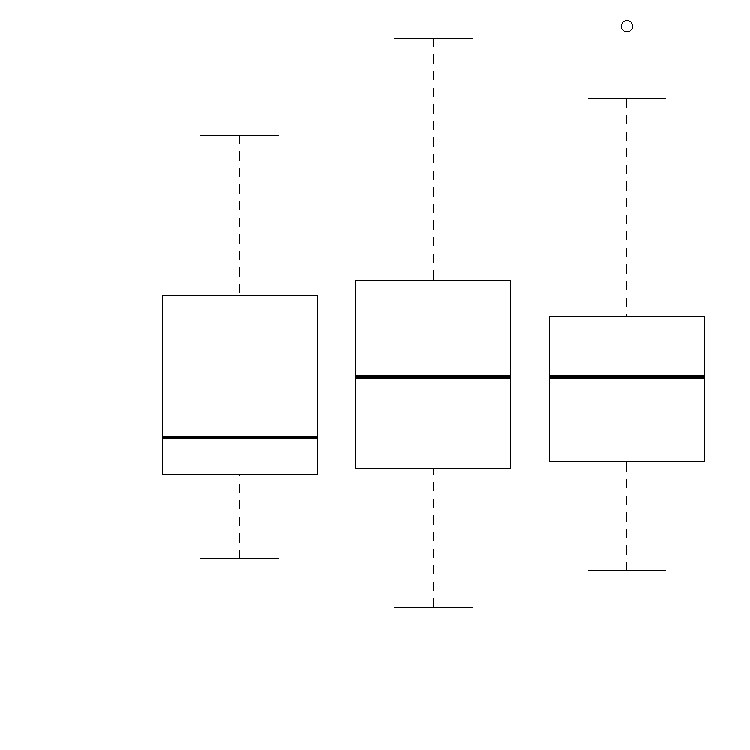
\includegraphics[width=\maxwidth]{figure/graphics-unnamed-chunk-213-1} 

}



\end{knitrout}


\begin{enumerate}
\item{} Costruire una funzione \texttt{inserisci} tale che il comando
$\texttt{inserisci}(\varia{x}, \varia{dove},\varia{cosa})$ inserisca nel vettore $\varia{x}$ l'elemento $\varia{cosa}$ nella posizione $\varia{dove}$.
Per esempio
\begin{knitrout}
\definecolor{shadecolor}{rgb}{0.969, 0.969, 0.969}\color{fgcolor}\begin{kframe}
\begin{alltt}
\hlstd{y} \hlkwb{<-}\hlstd{letters[}\hlnum{1}\hlopt{:}\hlnum{10}\hlstd{]}
\hlstd{y}
\end{alltt}
\begin{verbatim}
##  [1] "a" "b" "c" "d" "e" "f" "g" "h" "i"
## [10] "j"
\end{verbatim}
\end{kframe}
\end{knitrout}
\begin{knitrout}
\definecolor{shadecolor}{rgb}{0.969, 0.969, 0.969}\color{fgcolor}\begin{kframe}
\begin{alltt}
\hlkwd{inserisci}\hlstd{(x,} \hlnum{5}\hlstd{,} \hlnum{0}\hlstd{)}
\end{alltt}
\end{kframe}
\end{knitrout}
\begin{knitrout}
\definecolor{shadecolor}{rgb}{0.969, 0.969, 0.969}\color{fgcolor}\begin{kframe}
\begin{verbatim}
##  [1] "a" "b" "c" "d" "0" "e" "f" "g" "h"
## [10] "i" "j"
\end{verbatim}
\end{kframe}
\end{knitrout}
Generalizzare  al caso di inserimento di righe in \emph{dataframe}.
\item{}
Come si pu\`o verificare l'uguaglianza di 2 vettori includendo gli ingressi \texttt{NA}
\begin{knitrout}
\definecolor{shadecolor}{rgb}{0.969, 0.969, 0.969}\color{fgcolor}\begin{kframe}
\begin{alltt}
\hlnum{NA}\hlopt{==}\hlnum{NA}
\end{alltt}
\end{kframe}
\end{knitrout}
Aiuto: usare \texttt{is.na}
\item{}\cite{dalgaard}
Carichiamo il \emph{dataset} \texttt{juul} dal pacchetto \texttt{ISwR}. Ricavare il sottoinsieme di dati che corrispondono a ragazze tra i 7 e i 14 anni. Plottare \texttt{igf1} versus et\`a per ragazzi e ragazze separatamente. Conclusioni?
\end{enumerate}


\chapter{Operatori logici e selezione di elementi}
Consideriamo la selezione di elementi di un oggetto di \textsf{R}, per esempio \texttt{granchi}.
Selezioniamo per esempio tra i primi  50 i granchi con carapaci di lunghezza (sesta colonna) maggiore di 42:
\begin{knitrout}
\definecolor{shadecolor}{rgb}{0.969, 0.969, 0.969}\color{fgcolor}\begin{kframe}
\begin{alltt}
\hlkwd{data}\hlstd{(granchi)}
\hlstd{granchi[}\hlnum{1}\hlopt{:}\hlnum{50}\hlstd{,}\hlnum{6}\hlstd{]}\hlopt{>}\hlnum{42}
\end{alltt}
\begin{verbatim}
##  [1] FALSE FALSE FALSE FALSE FALSE FALSE
##  [7] FALSE FALSE FALSE FALSE FALSE FALSE
## [13] FALSE FALSE FALSE FALSE FALSE FALSE
## [19] FALSE FALSE FALSE FALSE FALSE FALSE
## [25] FALSE FALSE FALSE FALSE FALSE FALSE
## [31] FALSE FALSE FALSE FALSE FALSE FALSE
## [37] FALSE FALSE FALSE FALSE FALSE FALSE
## [43] FALSE  TRUE FALSE FALSE FALSE  TRUE
## [49]  TRUE  TRUE
\end{verbatim}
\end{kframe}
\end{knitrout}
Ciascun elemento del vettore viene confrontato con la soglia scelta (42) e quando supera la soglia la risposta \`e \texttt{TRUE} altrimenti \texttt{FALSE}.
\vskip20pt
%\begin{table}
\begin{tabular}
{|r r |}\hline
 \texttt{operatore}&  significato\\
\hline
\texttt{$>$}&  maggiore\\
\texttt{>=}& maggiore o uguale\\
\texttt{<}&   minore\\
\texttt{<=}&   minore o uguale\\
\texttt{==}&   uguale\\
\texttt{!=}&   diverso\\
\texttt{\&}&   and (e)\\
\texttt{|} & or (o)\\
\hline
\end{tabular}
\vskip20pt
%\end{table}
Gli ultimi due operatori combinano gli operatori precedenti. Per esempio
%code chunk
\begin{knitrout}
\definecolor{shadecolor}{rgb}{0.969, 0.969, 0.969}\color{fgcolor}\begin{kframe}
\begin{alltt}
\hlstd{crabs[crabs}\hlopt{$}\hlstd{sex} \hlopt{==} \hlstr{"F"} \hlopt{|} \hlstd{crabs}\hlopt{$}\hlstd{sp} \hlopt{==} \hlstr{"O"}\hlstd{,]}
\hlkwd{dim}\hlstd{(crabs[crabs}\hlopt{$}\hlstd{sex} \hlopt{==} \hlstr{"F"} \hlopt{&} \hlstd{crabs}\hlopt{$}\hlstd{sp} \hlopt{==} \hlstr{"O"}\hlstd{,])}
\end{alltt}
\end{kframe}
\end{knitrout}
%code chunk

\subsection{I valori non assegnati}
Capita frequentemente che un oggetto contenga valori non assegnati.
Per esempio
\begin{knitrout}
\definecolor{shadecolor}{rgb}{0.969, 0.969, 0.969}\color{fgcolor}\begin{kframe}
\begin{alltt}
\hlstd{x}\hlkwb{=}\hlnum{1}\hlstd{;x[}\hlnum{10}\hlstd{]}\hlkwb{=}\hlnum{4}\hlstd{;x}
\end{alltt}
\begin{verbatim}
##  [1]  1 NA NA NA NA NA NA NA NA  4
\end{verbatim}
\end{kframe}
\end{knitrout}
\begin{knitrout}
\definecolor{shadecolor}{rgb}{0.969, 0.969, 0.969}\color{fgcolor}\begin{kframe}
\begin{alltt}
\hlstd{x[}\hlopt{!}\hlkwd{is.na}\hlstd{(x)]}
\end{alltt}
\begin{verbatim}
## [1] 1 4
\end{verbatim}
\begin{alltt}
\hlkwd{class}\hlstd{(x)}
\end{alltt}
\begin{verbatim}
## [1] "numeric"
\end{verbatim}
\begin{alltt}
\hlkwd{class}\hlstd{(}\hlkwd{unclass}\hlstd{(x))}
\end{alltt}
\begin{verbatim}
## [1] "numeric"
\end{verbatim}
\begin{alltt}
\hlkwd{is.na}\hlstd{(x)}
\end{alltt}
\begin{verbatim}
##  [1] FALSE  TRUE  TRUE  TRUE  TRUE  TRUE
##  [7]  TRUE  TRUE  TRUE FALSE
\end{verbatim}
\begin{alltt}
 \hlstd{DF} \hlkwb{<-} \hlkwd{data.frame}\hlstd{(}\hlkwc{x} \hlstd{=} \hlkwd{c}\hlstd{(}\hlnum{1}\hlstd{,} \hlnum{2}\hlstd{,} \hlnum{3}\hlstd{),} \hlkwc{y} \hlstd{=} \hlkwd{c}\hlstd{(}\hlnum{0}\hlstd{,} \hlnum{10}\hlstd{,} \hlnum{NA}\hlstd{))}
\hlkwd{na.omit}\hlstd{(DF)}
\end{alltt}
\begin{verbatim}
##   x  y
## 1 1  0
## 2 2 10
\end{verbatim}
\begin{alltt}
\hlkwd{complete.cases}\hlstd{(x)}
\end{alltt}
\begin{verbatim}
##  [1]  TRUE FALSE FALSE FALSE FALSE FALSE
##  [7] FALSE FALSE FALSE  TRUE
\end{verbatim}
\end{kframe}
\end{knitrout}

\section{QQPlot
normality test}
\chapter{Grafica}
Il sistema grafico di \textsf{R} si compone di 3 parti: grafica di alto livello che produce grafici completi (per esempio \texttt{plot}, \texttt{curve}), grafica di basso livello che aggiunge elementi a grafici preesistenti (\texttt{text}, \texttt{abline}) e funzioni che lavorano interattivamente con grafici (ad esempio \texttt{locator()} e \texttt{identify()}).
\cite{murrell}.
A fianco della grafica tradizionale (gestita dal pacchetto \texttt{graphics}) esistono sistemi non tradizionali cui si pu\`o accedere attraverso il pacchetto \texttt{grid}. \index{\texttt{grid}}
In questo capitolo ci dedicheremo essenzialmente ad inquadrare la grafica tradizionale e daremo alcuni cenni sulla grafica non tradizionale.
\section{Le \emph{device} grafiche}
Le \emph{device} grafiche consentono di realizzare grafici di \textsf{R} su file di diversi formati (per esempio \texttt{.pdf}, \texttt{.ps}, \texttt{.bmp},\texttt{ .jpeg}, \texttt{.tiff}).
Il grafico anzich\'e essere  visualizzato a schermo, pu\`o quindi essere salvato direttamente in diversi formati. Per esempio il comando
\begin{knitrout}
\definecolor{shadecolor}{rgb}{0.969, 0.969, 0.969}\color{fgcolor}\begin{kframe}
\begin{alltt}
\hlkwd{pdf}\hlstd{(}\hlkwc{file} \hlstd{=} \hlstr{"miografico.pdf"}\hlstd{)}
\hlkwd{plot}\hlstd{(}\hlnum{1}\hlopt{:}\hlnum{10}\hlstd{)}
\hlkwd{dev.off}\hlstd{()}
\end{alltt}
\end{kframe}
\end{knitrout}
genera un file \texttt{.pdf} di nome \texttt{miografico} nella \emph{working directory}.
Se omettiamo il nome avremo il nome di defaults \texttt{Rplots}.
Per particolari \emph{device}  (per esempio \text{pdf}) la stampa su \emph{file} pu\`o occupare diverse pagine e quindi si possono inserire in un unico file diversi grafici.
Occorre ricordarsi di chiudere la \emph{device} al termine della produzione grafica con il comando \texttt{dev.off()}.
Il grafico sar\`a direttamente prodotto nel file indicato, dunque non si vedranno finestre grafiche e  apparir\`a  a schermo solo  un messaggio di avvenuta realizzazione del file una volta che la
\emph{device} viene chiusa.
La sintassi generica richiede dunque
\begin{enumerate}
\item{}Apertura della \emph{device} (definendone il nome, la dimensione
ed altri parametri non obbligatori, come la risoluzione)
\item{} Comandi grafici.
\item{} Chiusura della \emph{device}.
\end{enumerate}
Nota: le \emph{device} possono presentare piccole variazioni nei parametri, in particolare nei loro nomi. Un esempio: il nome del file in \texttt{png} \`e  definito dal parametro \texttt{filename=}, mentre nella device pdf \`e definito dal parametro \texttt{file=}. Consultare l'\emph{help} prima di utilizzarle non \`e  una cattiva idea. Tutti i parametri grafici visti valgono allo stesso modo per le \emph{device}.

\section{Lo stato grafico}
Ogni \emph{device} grafica mantiene uno stato grafico che viene consultato da \textsf{R} ogni volta che la \emph{device} viene usata. Lo stato grafico consiste in una serie di parametri specificabili con il comando \texttt{par}, nella forma
\begin{equation*}\texttt{par}(\varia{parametro}_1=\texttt{val}_1,\ldots)
\end{equation*}
Tecnicamente \texttt{par()} \`e una funzione  che restituisce una lista.
I parametri grafici specificabili con \texttt{par} sono ottenibili con il comando
\begin{knitrout}
\definecolor{shadecolor}{rgb}{0.969, 0.969, 0.969}\color{fgcolor}\begin{kframe}
\begin{alltt}
\hlkwd{options}\hlstd{(}\hlkwc{width}\hlstd{=}\hlnum{55}\hlstd{)}
\hlkwd{class}\hlstd{(}\hlkwd{par}\hlstd{())}
\end{alltt}
\begin{verbatim}
## [1] "list"
\end{verbatim}
\begin{alltt}
\hlkwd{names}\hlstd{(}\hlkwd{par}\hlstd{())}
\end{alltt}
\begin{verbatim}
##  [1] "xlog"      "ylog"      "adj"       "ann"      
##  [5] "ask"       "bg"        "bty"       "cex"      
##  [9] "cex.axis"  "cex.lab"   "cex.main"  "cex.sub"  
## [13] "cin"       "col"       "col.axis"  "col.lab"  
## [17] "col.main"  "col.sub"   "cra"       "crt"      
## [21] "csi"       "cxy"       "din"       "err"      
## [25] "family"    "fg"        "fig"       "fin"      
## [29] "font"      "font.axis" "font.lab"  "font.main"
## [33] "font.sub"  "lab"       "las"       "lend"     
## [37] "lheight"   "ljoin"     "lmitre"    "lty"      
## [41] "lwd"       "mai"       "mar"       "mex"      
## [45] "mfcol"     "mfg"       "mfrow"     "mgp"      
## [49] "mkh"       "new"       "oma"       "omd"      
## [53] "omi"       "page"      "pch"       "pin"      
## [57] "plt"       "ps"        "pty"       "smo"      
## [61] "srt"       "tck"       "tcl"       "usr"      
## [65] "xaxp"      "xaxs"      "xaxt"      "xpd"      
## [69] "yaxp"      "yaxs"      "yaxt"      "ylbias"
\end{verbatim}
\end{kframe}
\end{knitrout}
Per verificare lo stato grafico corrente basta scrivere \texttt{par()}. Per conoscere lo stato grafico di un particolare parametro basta scrivere $\texttt{par("\varia{nome parametro})"}$.
Ad esempio il parametro \texttt{bg} si riferisce al colore dello sfondo del grafico di default trasparente, mentre il parametro \texttt{lwd} si riferisce allo spessore delle linee.
Per cambiare i default dei due parametri
\begin{knitrout}
\definecolor{shadecolor}{rgb}{0.969, 0.969, 0.969}\color{fgcolor}\begin{kframe}
\begin{alltt}
\hlstd{oldpar}\hlkwb{<-}\hlkwd{par}\hlstd{(}\hlkwc{bg}\hlstd{=}\hlstr{"seashell1"}\hlstd{,}\hlstr{"lwd"}\hlstd{=}\hlnum{5}\hlstd{)}
\hlkwd{plot}\hlstd{(sin)}
\end{alltt}


{\ttfamily\noindent\bfseries\color{errorcolor}{\#\# Error in getMetricsFromLatex(TeXMetrics, verbose = verbose): \\\#\# TeX was unable to calculate metrics for the following string\\\#\# or character:\\\#\# \\\#\# 	m\\\#\# \\\#\# Common reasons for failure include:\\\#\#\ \  * The string contains a character which is special to LaTeX unless\\\#\#\ \ \ \  escaped properly, such as \% or \$.\\\#\#\ \  * The string makes use of LaTeX commands provided by a package and\\\#\#\ \ \ \  the tikzDevice was not told to load the package.\\\#\# \\\#\# The contents of the LaTeX log of the aborted run have been printed above,\\\#\# it may contain additional details as to why the metric calculation failed.}}\end{kframe}

{\centering 
\includegraphics[width=\maxwidth]{figure/graphics-unnamed-chunk-224-1} 

}



\end{knitrout}
Qui contestualmente alla ridefinizione abbiamo salvato (con il nome \texttt{oldpar}) la versione corrente dei parametri per poterli eventualmente ripristinare in seguito.
\begin{figure}\begin{center}
\begin{knitrout}
\definecolor{shadecolor}{rgb}{0.969, 0.969, 0.969}\color{fgcolor}\begin{kframe}


{\ttfamily\noindent\bfseries\color{errorcolor}{\#\# Error in getMetricsFromLatex(TeXMetrics, verbose = verbose): \\\#\# TeX was unable to calculate metrics for the following string\\\#\# or character:\\\#\# \\\#\# 	m\\\#\# \\\#\# Common reasons for failure include:\\\#\#\ \  * The string contains a character which is special to LaTeX unless\\\#\#\ \ \ \  escaped properly, such as \% or \$.\\\#\#\ \  * The string makes use of LaTeX commands provided by a package and\\\#\#\ \ \ \  the tikzDevice was not told to load the package.\\\#\# \\\#\# The contents of the LaTeX log of the aborted run have been printed above,\\\#\# it may contain additional details as to why the metric calculation failed.}}\end{kframe}

{\centering 
\includegraphics[width=\maxwidth]{figure/graphics-unnamed-chunk-225-1} 

}



\end{knitrout}
\caption{esempio di utilizzo di \texttt{par()}
}
\label{parbg}
\end{center}
\end{figure}
ottenendo la figura~\ref{parbg}.
Si noti che si possono riesumare i valori precedenti
\begin{knitrout}
\definecolor{shadecolor}{rgb}{0.969, 0.969, 0.969}\color{fgcolor}\begin{kframe}
\begin{alltt}
\hlkwd{par}\hlstd{(}\hlstr{"bg"}\hlstd{)}
\end{alltt}
\begin{verbatim}
## [1] "transparent"
\end{verbatim}
\begin{alltt}
\hlkwd{par}\hlstd{(oldpar)}
\hlkwd{par}\hlstd{(}\hlstr{"bg"}\hlstd{)}
\end{alltt}
\begin{verbatim}
## [1] "transparent"
\end{verbatim}
\end{kframe}
\end{knitrout}
\section{Elementi grafici di base}
\subsection{Costruzione di grafici multipli}
In questo capitolo disegneremo diversi grafici;  consideriamo preliminarmente la possibilit\`a di affiancarli in riga e in colonna, sia per ragioni di spazio che di chiarezza.
Per costruire tabelle di grafici in una finestra unica si usa il comando
\begin{equation*}
\texttt{par(mfrow=c}(\varia{nrighe},\varia{ncolonne}))
\end{equation*}
Per esempio  con una riga e due colonne
\begin{knitrout}
\definecolor{shadecolor}{rgb}{0.969, 0.969, 0.969}\color{fgcolor}\begin{kframe}
\begin{alltt}
\hlkwd{par}\hlstd{(}\hlkwc{mfrow}\hlstd{=}\hlkwd{c}\hlstd{(}\hlnum{1}\hlstd{,}\hlnum{2}\hlstd{))}
\hlkwd{plot}\hlstd{(iris[,}\hlnum{1}\hlstd{],iris[,}\hlnum{2}\hlstd{])}
\end{alltt}


{\ttfamily\noindent\bfseries\color{errorcolor}{\#\# Error in getMetricsFromLatex(TeXMetrics, verbose = verbose): \\\#\# TeX was unable to calculate metrics for the following string\\\#\# or character:\\\#\# \\\#\# 	m\\\#\# \\\#\# Common reasons for failure include:\\\#\#\ \  * The string contains a character which is special to LaTeX unless\\\#\#\ \ \ \  escaped properly, such as \% or \$.\\\#\#\ \  * The string makes use of LaTeX commands provided by a package and\\\#\#\ \ \ \  the tikzDevice was not told to load the package.\\\#\# \\\#\# The contents of the LaTeX log of the aborted run have been printed above,\\\#\# it may contain additional details as to why the metric calculation failed.}}\begin{alltt}
\hlkwd{plot}\hlstd{(iris[,}\hlnum{3}\hlstd{],iris[,}\hlnum{4}\hlstd{])}
\end{alltt}


{\ttfamily\noindent\bfseries\color{errorcolor}{\#\# Error in getMetricsFromLatex(TeXMetrics, verbose = verbose): \\\#\# TeX was unable to calculate metrics for the following string\\\#\# or character:\\\#\# \\\#\# 	m\\\#\# \\\#\# Common reasons for failure include:\\\#\#\ \  * The string contains a character which is special to LaTeX unless\\\#\#\ \ \ \  escaped properly, such as \% or \$.\\\#\#\ \  * The string makes use of LaTeX commands provided by a package and\\\#\#\ \ \ \  the tikzDevice was not told to load the package.\\\#\# \\\#\# The contents of the LaTeX log of the aborted run have been printed above,\\\#\# it may contain additional details as to why the metric calculation failed.}}\end{kframe}
\end{knitrout}
otteniamo i grafici affiancati della figura \ref{graficiaffiancati}.
\begin{figure}
\begin{center}
\begin{knitrout}
\definecolor{shadecolor}{rgb}{0.969, 0.969, 0.969}\color{fgcolor}\begin{kframe}


{\ttfamily\noindent\bfseries\color{errorcolor}{\#\# Error in getMetricsFromLatex(TeXMetrics, verbose = verbose): \\\#\# TeX was unable to calculate metrics for the following string\\\#\# or character:\\\#\# \\\#\# 	m\\\#\# \\\#\# Common reasons for failure include:\\\#\#\ \  * The string contains a character which is special to LaTeX unless\\\#\#\ \ \ \  escaped properly, such as \% or \$.\\\#\#\ \  * The string makes use of LaTeX commands provided by a package and\\\#\#\ \ \ \  the tikzDevice was not told to load the package.\\\#\# \\\#\# The contents of the LaTeX log of the aborted run have been printed above,\\\#\# it may contain additional details as to why the metric calculation failed.}}

{\ttfamily\noindent\bfseries\color{errorcolor}{\#\# Error in getMetricsFromLatex(TeXMetrics, verbose = verbose): \\\#\# TeX was unable to calculate metrics for the following string\\\#\# or character:\\\#\# \\\#\# 	m\\\#\# \\\#\# Common reasons for failure include:\\\#\#\ \  * The string contains a character which is special to LaTeX unless\\\#\#\ \ \ \  escaped properly, such as \% or \$.\\\#\#\ \  * The string makes use of LaTeX commands provided by a package and\\\#\#\ \ \ \  the tikzDevice was not told to load the package.\\\#\# \\\#\# The contents of the LaTeX log of the aborted run have been printed above,\\\#\# it may contain additional details as to why the metric calculation failed.}}\end{kframe}

{\centering 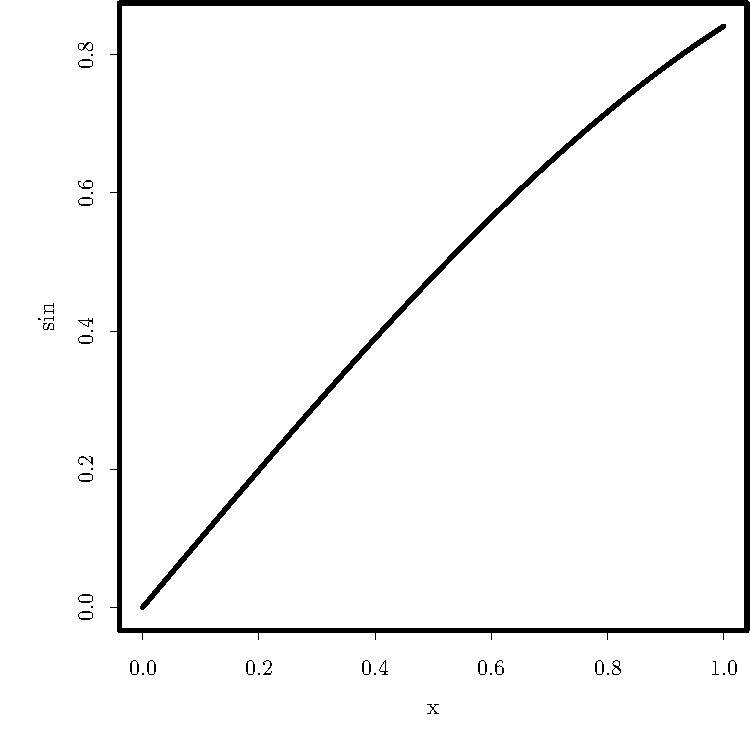
\includegraphics[width=\maxwidth]{figure/graphics-unnamed-chunk-228-1} 

}



\end{knitrout}
\caption{Grafici affiancati con \texttt{mfrow=c(1,2)}}
\label{fig:graficiaffiancati}
\end{center}
\end{figure}

\subsection{Diagrammi a dispersione}
La sintassi di riferimento della funzione \texttt{plot} \index{\texttt{plot}} \`e
\begin{equation*}
\texttt{plot}(\varia{dati},\varia{opzione}_1=val_1, \varia{opzione}_2=val_2,\ldots,\varia{opzione}_n=val_n)\end{equation*}
Scarichiamo da \cite{dasl} il \emph{dataset} che chiameremo \texttt{Gompertz} in cui si studia la mortalit\`a di una popolazione di moscerini al variare dell'et\`a
%code chunk

\begin{knitrout}
\definecolor{shadecolor}{rgb}{0.969, 0.969, 0.969}\color{fgcolor}\begin{kframe}
\begin{alltt}
\hlstd{url}\hlkwb{=}\hlstr{"http://lib.stat.cmu.edu/DASL/Datafiles/Medflies.html"}
\hlstd{gompertz}\hlkwb{<-}\hlkwd{read.table}\hlstd{(url,}\hlkwc{skip}\hlstd{=}\hlnum{25}\hlstd{,}\hlkwc{nrow}\hlstd{=}\hlnum{173}\hlstd{,}\hlkwc{header}\hlstd{=T)}
\end{alltt}
\end{kframe}
\end{knitrout}
\begin{knitrout}
\definecolor{shadecolor}{rgb}{0.969, 0.969, 0.969}\color{fgcolor}\begin{kframe}
\begin{alltt}
\hlkwd{class}\hlstd{(gompertz)}
\end{alltt}
\begin{verbatim}
## [1] "data.frame"
\end{verbatim}
\begin{alltt}
\hlkwd{head}\hlstd{(gompertz)}
\end{alltt}
\begin{verbatim}
##   day  living mort.rate
## 1   0 1203646         0
## 2   1 1203646    0.0014
## 3   2 1201913    0.0040
## 4   3 1197098    0.0051
## 5   4 1191020    0.0064
## 6   5 1183419    0.0075
\end{verbatim}
\begin{alltt}
\hlkwd{par}\hlstd{(}\hlkwc{mfrow}\hlstd{=}\hlkwd{c}\hlstd{(}\hlnum{1}\hlstd{,}\hlnum{2}\hlstd{))}
\hlkwd{plot}\hlstd{(gompertz[,}\hlnum{1}\hlstd{],gompertz[,}\hlnum{2}\hlstd{])}
\end{alltt}


{\ttfamily\noindent\bfseries\color{errorcolor}{\#\# Error in getMetricsFromLatex(TeXMetrics, verbose = verbose): \\\#\# TeX was unable to calculate metrics for the following string\\\#\# or character:\\\#\# \\\#\# 	m\\\#\# \\\#\# Common reasons for failure include:\\\#\#\ \  * The string contains a character which is special to LaTeX unless\\\#\#\ \ \ \  escaped properly, such as \% or \$.\\\#\#\ \  * The string makes use of LaTeX commands provided by a package and\\\#\#\ \ \ \  the tikzDevice was not told to load the package.\\\#\# \\\#\# The contents of the LaTeX log of the aborted run have been printed above,\\\#\# it may contain additional details as to why the metric calculation failed.}}\begin{alltt}
\hlkwd{plot}\hlstd{(gompertz[,}\hlnum{1}\hlstd{],gompertz[,}\hlnum{3}\hlstd{])}
\end{alltt}


{\ttfamily\noindent\color{warningcolor}{\#\# Warning in xy.coords(x, y, xlabel, ylabel, log): NAs introduced by coercion}}

{\ttfamily\noindent\bfseries\color{errorcolor}{\#\# Error in getMetricsFromLatex(TeXMetrics, verbose = verbose): \\\#\# TeX was unable to calculate metrics for the following string\\\#\# or character:\\\#\# \\\#\# 	m\\\#\# \\\#\# Common reasons for failure include:\\\#\#\ \  * The string contains a character which is special to LaTeX unless\\\#\#\ \ \ \  escaped properly, such as \% or \$.\\\#\#\ \  * The string makes use of LaTeX commands provided by a package and\\\#\#\ \ \ \  the tikzDevice was not told to load the package.\\\#\# \\\#\# The contents of the LaTeX log of the aborted run have been printed above,\\\#\# it may contain additional details as to why the metric calculation failed.}}\end{kframe}

{\centering 
\includegraphics[width=\maxwidth]{figure/graphics-unnamed-chunk-231-1} 

}



\end{knitrout}

\begin{figure}\begin{center}
\begin{knitrout}
\definecolor{shadecolor}{rgb}{0.969, 0.969, 0.969}\color{fgcolor}\begin{kframe}


{\ttfamily\noindent\bfseries\color{errorcolor}{\#\# Error in getMetricsFromLatex(TeXMetrics, verbose = verbose): \\\#\# TeX was unable to calculate metrics for the following string\\\#\# or character:\\\#\# \\\#\# 	m\\\#\# \\\#\# Common reasons for failure include:\\\#\#\ \  * The string contains a character which is special to LaTeX unless\\\#\#\ \ \ \  escaped properly, such as \% or \$.\\\#\#\ \  * The string makes use of LaTeX commands provided by a package and\\\#\#\ \ \ \  the tikzDevice was not told to load the package.\\\#\# \\\#\# The contents of the LaTeX log of the aborted run have been printed above,\\\#\# it may contain additional details as to why the metric calculation failed.}}

{\ttfamily\noindent\color{warningcolor}{\#\# Warning in xy.coords(x, y, xlabel, ylabel, log): NAs introduced by coercion}}

{\ttfamily\noindent\bfseries\color{errorcolor}{\#\# Error in getMetricsFromLatex(TeXMetrics, verbose = verbose): \\\#\# TeX was unable to calculate metrics for the following string\\\#\# or character:\\\#\# \\\#\# 	m\\\#\# \\\#\# Common reasons for failure include:\\\#\#\ \  * The string contains a character which is special to LaTeX unless\\\#\#\ \ \ \  escaped properly, such as \% or \$.\\\#\#\ \  * The string makes use of LaTeX commands provided by a package and\\\#\#\ \ \ \  the tikzDevice was not told to load the package.\\\#\# \\\#\# The contents of the LaTeX log of the aborted run have been printed above,\\\#\# it may contain additional details as to why the metric calculation failed.}}\end{kframe}

{\centering 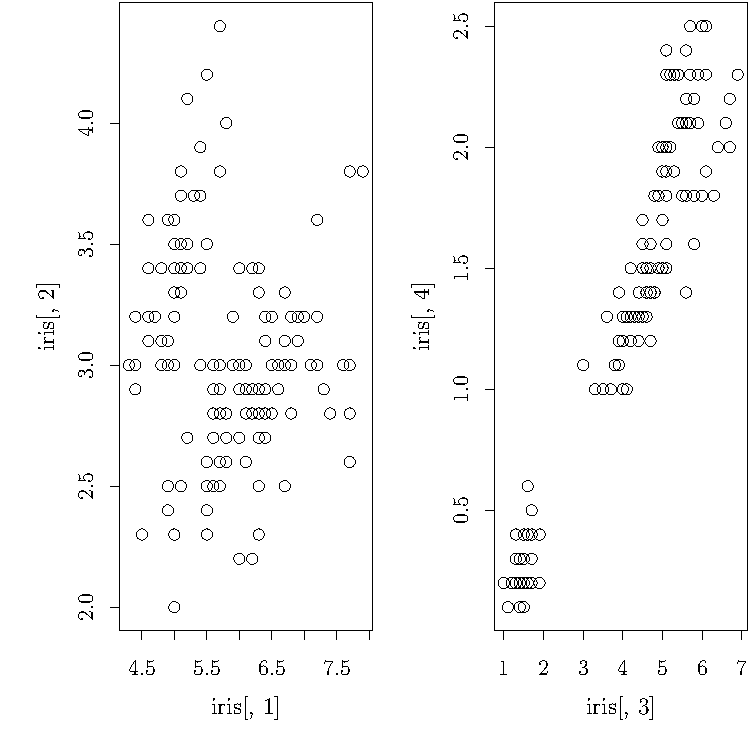
\includegraphics[width=\maxwidth]{figure/graphics-unnamed-chunk-232-1} 

}



\end{knitrout}
\caption{Mortalit\`a dei moscerini. A sinistra la decrescita della popolazione, a destra la mortalit\`a.}
\label{moscerini}
\end{center}
\end{figure}
Il tasso di mortalit\`a (\texttt{mort.rate}) all'istante $t_1$ \`e definito  come rapporto tra numero di individui deceduti nell'intervallo di tempo  $(t_1,t_1+1)$ e  numero di individui all'istante $t_1$. Il comando \texttt{diff} \index{\texttt{diff}} applicato ad una lista ne calcola le differenze termine a termine.
Per esempio
\begin{knitrout}
\definecolor{shadecolor}{rgb}{0.969, 0.969, 0.969}\color{fgcolor}\begin{kframe}
\begin{alltt}
\hlkwd{diff}\hlstd{(}\hlnum{2}\hlopt{^}\hlstd{(}\hlnum{1}\hlopt{:}\hlnum{10}\hlstd{))}
\end{alltt}
\begin{verbatim}
## [1]   2   4   8  16  32  64 128 256 512
\end{verbatim}
\end{kframe}
\end{knitrout}
Il comando che segue consente quindi di verificare la terza colonna di Gompertz
\begin{knitrout}
\definecolor{shadecolor}{rgb}{0.969, 0.969, 0.969}\color{fgcolor}\begin{kframe}
\begin{alltt}
\hlkwd{head}\hlstd{(}\hlopt{-}\hlkwd{diff}\hlstd{(gompertz[,}\hlnum{2}\hlstd{])}\hlopt{/}\hlstd{gompertz[}\hlopt{-}\hlnum{1}\hlstd{,}\hlnum{2}\hlstd{])}
\end{alltt}
\begin{verbatim}
## [1] 0.000000000 0.001441868 0.004022227 0.005103189
## [5] 0.006422915 0.007592154
\end{verbatim}
\end{kframe}
\end{knitrout}

Alcune opzioni che possono perfezionare un grafico sono
\begin{itemize}
\item{}\texttt{main}=: assegna il titolo al grafico;
\item{}\texttt{xlab}=: assegna l'etichetta all'asse delle $x$;
\item{}\texttt{ylab}=: assegna l'etichetta all'asse delle $y$;
\item{}\texttt{type}=:
\begin{itemize}
\item{} \texttt{p} Disegna solo i punti.
\item{} \texttt{l} Disegna linee.
\item{} \texttt{b} Disegna entrambi ma senza
sovrapporre le linee ai punti.
\item{} \texttt{o} Disegna linee e punti ma sovrapposti.
\item{} \texttt{n} Non disegna n\'e linee n\'e punti. Serve talora a impostare la finestra grafica.
\end{itemize}
\item{} \texttt{col}=: assegna il colore il cui elenco si ottiene con il comando: \texttt{colors()};
\item{} \texttt{cex}=: un valore numerico, da 0 (sopprime i punti) a valori numerici consigliati minori di 2, definisce la dimensione dei punti;
\item{}\texttt{lty}=: definisce il tipo di linea ({\it line type}), se 1 linea continua, se 2 tratteggiata, se 3 tratteggiata con tratto ridotto, se 4 tratto e punto;
\item{}\texttt{lwd}=: definisce lo spessore della linea ({\it line width}), valori suggeriti tra 0.5 e 2;
\item{} \texttt{pch}=: definisce il \emph{marker} dei punti
\end{itemize}
\footnote{Si noti che tali opzioni coincidono in alcuni casi con opzioni specificabili con \texttt{par}.  In questo caso sono per\`o solo locali. }

Per esempio
\begin{knitrout}
\definecolor{shadecolor}{rgb}{0.969, 0.969, 0.969}\color{fgcolor}\begin{kframe}
\begin{alltt}
\hlkwd{par}\hlstd{(}\hlkwc{mfrow}\hlstd{=}\hlkwd{c}\hlstd{(}\hlnum{2}\hlstd{,}\hlnum{2}\hlstd{))}
\hlstd{gompertz[,}\hlkwd{c}\hlstd{(}\hlnum{1}\hlstd{,}\hlnum{3}\hlstd{)]}\hlkwb{->}\hlstd{dati}
\hlkwd{plot}\hlstd{(dati,}\hlkwc{main}\hlstd{=}\hlstr{"La mortalit\textbackslash{}uE5 dei moscerini"}\hlstd{,} \hlkwc{xlab}\hlstd{=}\hlstr{"t (giorni)"}\hlstd{,}
\hlkwc{ylab}\hlstd{=}\hlstr{"Tasso di mortalit\textbackslash{}uE5"}\hlstd{)}
\hlkwd{plot}\hlstd{(dati,}\hlkwc{main}\hlstd{=}\hlstr{"La mortalit\textbackslash{}uE5 dei moscerini"}\hlstd{,} \hlkwc{xlab}\hlstd{=}\hlstr{"t (giorni)"}\hlstd{,}
\hlkwc{ylab}\hlstd{=}\hlstr{"Tasso di mortalit\textbackslash{}uE5"}\hlstd{,}\hlkwc{type}\hlstd{=}\hlstr{"l"}\hlstd{)}
\hlkwd{plot}\hlstd{(dati,}\hlkwc{main}\hlstd{=}\hlstr{"La mortalit\textbackslash{}uE5 dei moscerini"}\hlstd{,} \hlkwc{xlab}\hlstd{=}\hlstr{"t (giorni)"}\hlstd{,}
\hlkwc{ylab}\hlstd{=}\hlstr{"Tasso di mortalit\textbackslash{}uE5"}\hlstd{,} \hlkwc{col}\hlstd{=}\hlstr{"dark green"}\hlstd{,}\hlkwc{cex}\hlstd{=}\hlnum{0.5}\hlstd{)}
\hlkwd{plot}\hlstd{(dati,}\hlkwc{main}\hlstd{=}\hlstr{"La mortalit\textbackslash{}uE5 dei moscerini"}\hlstd{,} \hlkwc{xlab}\hlstd{=}\hlstr{"t (giorni)"}\hlstd{,}
\hlkwc{ylab}\hlstd{=}\hlstr{"Tasso di mortalit\textbackslash{}uE5"}\hlstd{,} \hlkwc{col}\hlstd{=}\hlstr{"dark green"}\hlstd{,}\hlkwc{cex}\hlstd{=}\hlnum{0.5}\hlstd{,}
\hlkwc{lty}\hlstd{=}\hlnum{4}\hlstd{,}\hlkwc{lwd}\hlstd{=}\hlnum{2}\hlstd{)}
\end{alltt}
\end{kframe}
\end{knitrout}
Il risultato \`e riportato nella figura~\ref{4moscerini}
\begin{figure}\begin{center}
\begin{knitrout}
\definecolor{shadecolor}{rgb}{0.969, 0.969, 0.969}\color{fgcolor}\begin{kframe}


{\ttfamily\noindent\color{warningcolor}{\#\# Warning in xy.coords(x, y, xlabel, ylabel, log): NAs introduced by coercion}}

{\ttfamily\noindent\bfseries\color{errorcolor}{\#\# Error in getMetricsFromLatex(TeXMetrics, verbose = verbose): \\\#\# TeX was unable to calculate metrics for the following string\\\#\# or character:\\\#\# \\\#\# 	m\\\#\# \\\#\# Common reasons for failure include:\\\#\#\ \  * The string contains a character which is special to LaTeX unless\\\#\#\ \ \ \  escaped properly, such as \% or \$.\\\#\#\ \  * The string makes use of LaTeX commands provided by a package and\\\#\#\ \ \ \  the tikzDevice was not told to load the package.\\\#\# \\\#\# The contents of the LaTeX log of the aborted run have been printed above,\\\#\# it may contain additional details as to why the metric calculation failed.}}

{\ttfamily\noindent\color{warningcolor}{\#\# Warning in xy.coords(x, y, xlabel, ylabel, log): NAs introduced by coercion}}

{\ttfamily\noindent\bfseries\color{errorcolor}{\#\# Error in getMetricsFromLatex(TeXMetrics, verbose = verbose): \\\#\# TeX was unable to calculate metrics for the following string\\\#\# or character:\\\#\# \\\#\# 	m\\\#\# \\\#\# Common reasons for failure include:\\\#\#\ \  * The string contains a character which is special to LaTeX unless\\\#\#\ \ \ \  escaped properly, such as \% or \$.\\\#\#\ \  * The string makes use of LaTeX commands provided by a package and\\\#\#\ \ \ \  the tikzDevice was not told to load the package.\\\#\# \\\#\# The contents of the LaTeX log of the aborted run have been printed above,\\\#\# it may contain additional details as to why the metric calculation failed.}}

{\ttfamily\noindent\color{warningcolor}{\#\# Warning in xy.coords(x, y, xlabel, ylabel, log): NAs introduced by coercion}}

{\ttfamily\noindent\bfseries\color{errorcolor}{\#\# Error in getMetricsFromLatex(TeXMetrics, verbose = verbose): \\\#\# TeX was unable to calculate metrics for the following string\\\#\# or character:\\\#\# \\\#\# 	m\\\#\# \\\#\# Common reasons for failure include:\\\#\#\ \  * The string contains a character which is special to LaTeX unless\\\#\#\ \ \ \  escaped properly, such as \% or \$.\\\#\#\ \  * The string makes use of LaTeX commands provided by a package and\\\#\#\ \ \ \  the tikzDevice was not told to load the package.\\\#\# \\\#\# The contents of the LaTeX log of the aborted run have been printed above,\\\#\# it may contain additional details as to why the metric calculation failed.}}

{\ttfamily\noindent\color{warningcolor}{\#\# Warning in xy.coords(x, y, xlabel, ylabel, log): NAs introduced by coercion}}

{\ttfamily\noindent\bfseries\color{errorcolor}{\#\# Error in getMetricsFromLatex(TeXMetrics, verbose = verbose): \\\#\# TeX was unable to calculate metrics for the following string\\\#\# or character:\\\#\# \\\#\# 	m\\\#\# \\\#\# Common reasons for failure include:\\\#\#\ \  * The string contains a character which is special to LaTeX unless\\\#\#\ \ \ \  escaped properly, such as \% or \$.\\\#\#\ \  * The string makes use of LaTeX commands provided by a package and\\\#\#\ \ \ \  the tikzDevice was not told to load the package.\\\#\# \\\#\# The contents of the LaTeX log of the aborted run have been printed above,\\\#\# it may contain additional details as to why the metric calculation failed.}}\end{kframe}

{\centering 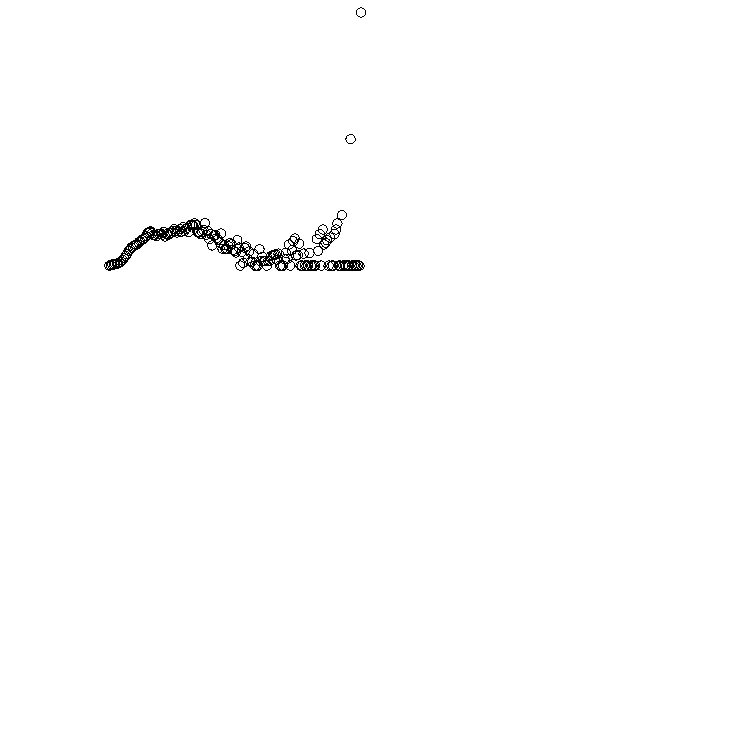
\includegraphics[width=\maxwidth]{figure/graphics-unnamed-chunk-236-1} 

}



\end{knitrout}
\caption{Utilizzo di diversi parametri grafici}
\label{4moscerini}
\end{center}
\end{figure}





\subsection{Grafici multipli e/o sovrapposti}

Analizziamo il {\it dataframe} \texttt{quakes} che riporta numerosi dati sui terremoti che colpiscono la zona delle isole Fiji.
Carichiamo i dati e utilizziamo la funzione \texttt{pairs}\index{pairs} per costruire grafici multipli in un'unica finestra:
\begin{knitrout}
\definecolor{shadecolor}{rgb}{0.969, 0.969, 0.969}\color{fgcolor}\begin{kframe}
\begin{alltt}
\hlstd{quakes}
\hlkwd{pairs}\hlstd{(quakes,} \hlkwc{main} \hlstd{=} \hlstr{"Fiji Earthquakes, N = 1000"}\hlstd{,} \hlkwc{cex.main}\hlstd{=}\hlnum{1.2}\hlstd{,} \hlkwc{pch}\hlstd{=}\hlstr{"."}\hlstd{)}
\end{alltt}


{\ttfamily\noindent\bfseries\color{errorcolor}{\#\# Error in getMetricsFromLatex(TeXMetrics, verbose = verbose): \\\#\# TeX was unable to calculate metrics for the following string\\\#\# or character:\\\#\# \\\#\# 	lat\\\#\# \\\#\# Common reasons for failure include:\\\#\#\ \  * The string contains a character which is special to LaTeX unless\\\#\#\ \ \ \  escaped properly, such as \% or \$.\\\#\#\ \  * The string makes use of LaTeX commands provided by a package and\\\#\#\ \ \ \  the tikzDevice was not told to load the package.\\\#\# \\\#\# The contents of the LaTeX log of the aborted run have been printed above,\\\#\# it may contain additional details as to why the metric calculation failed.}}\end{kframe}
\end{knitrout}

\begin{center}
\begin{figure}
\begin{knitrout}
\definecolor{shadecolor}{rgb}{0.969, 0.969, 0.969}\color{fgcolor}\begin{kframe}


{\ttfamily\noindent\bfseries\color{errorcolor}{\#\# Error in getMetricsFromLatex(TeXMetrics, verbose = verbose): \\\#\# TeX was unable to calculate metrics for the following string\\\#\# or character:\\\#\# \\\#\# 	lat\\\#\# \\\#\# Common reasons for failure include:\\\#\#\ \  * The string contains a character which is special to LaTeX unless\\\#\#\ \ \ \  escaped properly, such as \% or \$.\\\#\#\ \  * The string makes use of LaTeX commands provided by a package and\\\#\#\ \ \ \  the tikzDevice was not told to load the package.\\\#\# \\\#\# The contents of the LaTeX log of the aborted run have been printed above,\\\#\# it may contain additional details as to why the metric calculation failed.}}\end{kframe}

{\centering 
\includegraphics[width=\maxwidth]{figure/graphics-unnamed-chunk-238-1} 

}



\end{knitrout}
\caption{Plot per variabili multiple}
\label{pairplot}
\end{figure}
\end{center}
In effetti il comando \texttt{plot} funziona anche su \emph{dataframe} come \`e verificabile con
\begin{knitrout}
\definecolor{shadecolor}{rgb}{0.969, 0.969, 0.969}\color{fgcolor}\begin{kframe}
\begin{alltt}
\hlkwd{methods}\hlstd{(plot)}
\end{alltt}
\begin{verbatim}
##  [1] plot,ANY-method      plot,Funzione-method
##  [3] plot.acf*            plot.correspondence*
##  [5] plot.data.frame*     plot.decomposed.ts* 
##  [7] plot.default         plot.dendrogram*    
##  [9] plot.density*        plot.ecdf           
## [11] plot.factor*         plot.formula*       
## [13] plot.function        plot.hclust*        
## [15] plot.histogram*      plot.HoltWinters*   
## [17] plot.isoreg*         plot.lda*           
## [19] plot.lm*             plot.mca*           
## [21] plot.medpolish*      plot.mlm*           
## [23] plot.ppr*            plot.prcomp*        
## [25] plot.princomp*       plot.profile*       
## [27] plot.profile.nls*    plot.raster*        
## [29] plot.ridgelm*        plot.spec*          
## [31] plot.stepfun         plot.stl*           
## [33] plot.table*          plot.ts             
## [35] plot.tskernel*       plot.TukeyHSD*      
## see '?methods' for accessing help and source code
\end{verbatim}
\end{kframe}
\end{knitrout}
e produce lo stesso risultato.
Il grafico risulta complesso da comprendere anche per via delle ridotte dimensioni. Selezioniamo solo i dati relativi alla longitudine ed alla latitudine (prime 2 colonne):
\begin{knitrout}
\definecolor{shadecolor}{rgb}{0.969, 0.969, 0.969}\color{fgcolor}\begin{kframe}
\begin{alltt}
 \hlkwd{plot}\hlstd{(quakes[,}\hlkwd{c}\hlstd{(}\hlnum{1}\hlstd{,}\hlnum{2}\hlstd{)],} \hlkwc{main} \hlstd{=} \hlstr{"Fiji Earthquakes, N = 1000"}\hlstd{,} \hlkwc{cex.main}\hlstd{=}\hlnum{1.2}\hlstd{,} \hlkwc{pch}\hlstd{=}\hlstr{"."}\hlstd{)}
\end{alltt}


{\ttfamily\noindent\bfseries\color{errorcolor}{\#\# Error in getMetricsFromLatex(TeXMetrics, verbose = verbose): \\\#\# TeX was unable to calculate metrics for the following string\\\#\# or character:\\\#\# \\\#\# 	m\\\#\# \\\#\# Common reasons for failure include:\\\#\#\ \  * The string contains a character which is special to LaTeX unless\\\#\#\ \ \ \  escaped properly, such as \% or \$.\\\#\#\ \  * The string makes use of LaTeX commands provided by a package and\\\#\#\ \ \ \  the tikzDevice was not told to load the package.\\\#\# \\\#\# The contents of the LaTeX log of the aborted run have been printed above,\\\#\# it may contain additional details as to why the metric calculation failed.}}\end{kframe}

{\centering 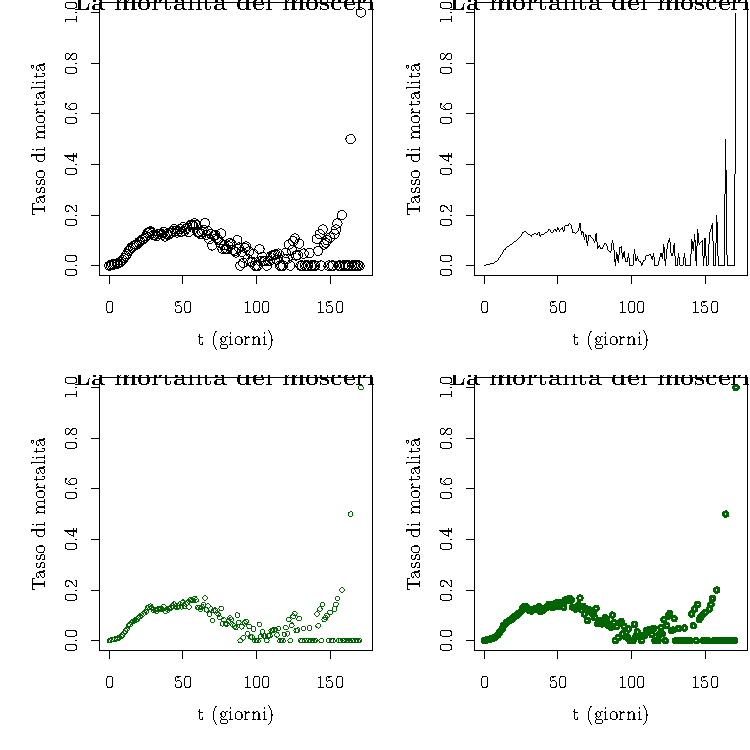
\includegraphics[width=\maxwidth]{figure/graphics-unnamed-chunk-240-1} 

}



\end{knitrout}
\ese{Migliorare questi grafici secondo il gusto personale inserendo, titoli, colorazioni, sfondo, tipo di rappresentazione, tipo di punti, etc.}
\subsection{Aggiungere testo al grafico}
Si pu\`o aggiungere testo in qualunque posizione del grafico, in particolare possiamo posizionare commenti, annotazioni, formule, ecc. Si devono solo specificare coordinate e testo, oltre ad altri parametri visualizzabili con \texttt{?text}.
Nell'esempio seguente generiamo i vertici di un poligono regolare con numero di lati uguali al numero di lettere dell'alfabeto.
\begin{knitrout}
\definecolor{shadecolor}{rgb}{0.969, 0.969, 0.969}\color{fgcolor}\begin{kframe}
\begin{alltt}
\hlkwd{set.seed}\hlstd{(}\hlnum{20}\hlstd{)}\hlcom{#inizializza il generatore}
\hlstd{nl}\hlkwb{=}\hlkwd{length}\hlstd{(letters)}\hlcom{#numero di lettere}
\hlstd{coord.poli}\hlkwb{=}\hlkwd{matrix}\hlstd{(}\hlkwd{c}\hlstd{(}\hlkwd{cos}\hlstd{(}\hlnum{2}\hlopt{*} \hlstd{pi} \hlopt{*}\hlstd{(}\hlnum{1}\hlopt{:}\hlstd{nl)}\hlopt{/}\hlstd{nl),} \hlkwd{sin} \hlstd{(}\hlnum{2}\hlopt{*}\hlstd{pi}\hlopt{*}\hlstd{(}\hlnum{1}\hlopt{:}\hlstd{nl)}\hlopt{/}\hlstd{nl)),}
\hlkwc{nc}\hlstd{=}\hlnum{2}\hlstd{,}\hlkwc{nrow}\hlstd{=nl);}\hlcom{#vertici del poligono}
\hlstd{coord.random}\hlkwb{<-}\hlkwd{matrix}\hlstd{(}\hlkwd{runif}\hlstd{(}\hlnum{2}\hlopt{*}\hlstd{nl),}\hlkwc{nc}\hlstd{=}\hlnum{2}\hlstd{,}\hlkwc{nrow}\hlstd{=nl)}\hlcom{#perturbazione}
\hlstd{coord}\hlkwb{=}\hlstd{coord.random}\hlopt{+}\hlnum{3}\hlopt{*}\hlstd{coord.poli;}\hlcom{#coordinate perturbate}
\hlcom{#plot(coord,col="blue",lwd=4,lty=1,type="l")}
\hlcom{#text(coord,letters,col="red",cex=1.6,adj=2)#inserimento del testo}
\hlkwd{plot}\hlstd{(coord,}\hlkwc{col}\hlstd{=}\hlstr{"blue"}\hlstd{,}\hlkwc{lwd}\hlstd{=}\hlnum{4}\hlstd{,}\hlkwc{lty}\hlstd{=}\hlnum{1}\hlstd{,}\hlkwc{type}\hlstd{=}\hlstr{"n"}\hlstd{)}
\end{alltt}


{\ttfamily\noindent\bfseries\color{errorcolor}{\#\# Error in getMetricsFromLatex(TeXMetrics, verbose = verbose): \\\#\# TeX was unable to calculate metrics for the following string\\\#\# or character:\\\#\# \\\#\# 	m\\\#\# \\\#\# Common reasons for failure include:\\\#\#\ \  * The string contains a character which is special to LaTeX unless\\\#\#\ \ \ \  escaped properly, such as \% or \$.\\\#\#\ \  * The string makes use of LaTeX commands provided by a package and\\\#\#\ \ \ \  the tikzDevice was not told to load the package.\\\#\# \\\#\# The contents of the LaTeX log of the aborted run have been printed above,\\\#\# it may contain additional details as to why the metric calculation failed.}}\begin{alltt}
\hlkwd{polygon}\hlstd{(coord,}\hlkwc{col}\hlstd{=}\hlstr{"yellow"}\hlstd{,}\hlkwc{density}\hlstd{=}\hlnum{10}\hlstd{,}\hlkwc{angle}\hlstd{=}\hlnum{30}\hlstd{)}
\hlkwd{text}\hlstd{(coord,letters,}\hlkwc{col}\hlstd{=}\hlstr{"red"}\hlstd{)}
\end{alltt}


{\ttfamily\noindent\bfseries\color{errorcolor}{\#\# Error in getMetricsFromLatex(TeXMetrics, verbose = verbose): \\\#\# TeX was unable to calculate metrics for the following string\\\#\# or character:\\\#\# \\\#\# 	a\\\#\# \\\#\# Common reasons for failure include:\\\#\#\ \  * The string contains a character which is special to LaTeX unless\\\#\#\ \ \ \  escaped properly, such as \% or \$.\\\#\#\ \  * The string makes use of LaTeX commands provided by a package and\\\#\#\ \ \ \  the tikzDevice was not told to load the package.\\\#\# \\\#\# The contents of the LaTeX log of the aborted run have been printed above,\\\#\# it may contain additional details as to why the metric calculation failed.}}\end{kframe}

{\centering \includegraphics[width=\maxwidth]{figure/graphics-unnamed-chunk-241-1} 

}



\end{knitrout}

Il parametro  \texttt{adj} sposta il testo rispetto alle coordinate
\subsection{Immagini di un vulcano}
Vediamo alcune rappresentazioni grafiche 3D.
\begin{knitrout}
\definecolor{shadecolor}{rgb}{0.969, 0.969, 0.969}\color{fgcolor}\begin{kframe}
\begin{alltt}
\hlcom{#require(grDevices);}
\hlcom{#require(graphics)}
\hlkwd{filled.contour}\hlstd{(volcano,} \hlkwc{color.palette} \hlstd{= terrain.colors,} \hlkwc{asp} \hlstd{=} \hlnum{1}\hlstd{)}
\end{alltt}


{\ttfamily\noindent\bfseries\color{errorcolor}{\#\# Error in getMetricsFromLatex(TeXMetrics, verbose = verbose): \\\#\# TeX was unable to calculate metrics for the following string\\\#\# or character:\\\#\# \\\#\# 	m\\\#\# \\\#\# Common reasons for failure include:\\\#\#\ \  * The string contains a character which is special to LaTeX unless\\\#\#\ \ \ \  escaped properly, such as \% or \$.\\\#\#\ \  * The string makes use of LaTeX commands provided by a package and\\\#\#\ \ \ \  the tikzDevice was not told to load the package.\\\#\# \\\#\# The contents of the LaTeX log of the aborted run have been printed above,\\\#\# it may contain additional details as to why the metric calculation failed.}}\begin{alltt}
\hlkwd{title}\hlstd{(}\hlkwc{main} \hlstd{=} \hlstr{"volcano data: filled contour map"}\hlstd{)}
\end{alltt}


{\ttfamily\noindent\bfseries\color{errorcolor}{\#\# Error in getMetricsFromLatex(TeXMetrics, verbose = verbose): \\\#\# TeX was unable to calculate metrics for the following string\\\#\# or character:\\\#\# \\\#\# 	volcano data: filled contour map\\\#\# \\\#\# Common reasons for failure include:\\\#\#\ \  * The string contains a character which is special to LaTeX unless\\\#\#\ \ \ \  escaped properly, such as \% or \$.\\\#\#\ \  * The string makes use of LaTeX commands provided by a package and\\\#\#\ \ \ \  the tikzDevice was not told to load the package.\\\#\# \\\#\# The contents of the LaTeX log of the aborted run have been printed above,\\\#\# it may contain additional details as to why the metric calculation failed.}}\end{kframe}

{\centering 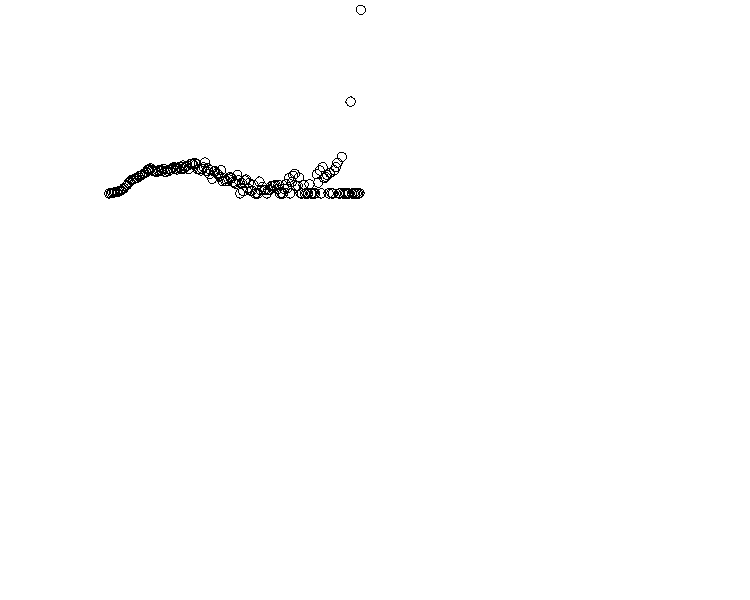
\includegraphics[width=\maxwidth]{figure/graphics-unnamed-chunk-242-1} 

}



\end{knitrout}
\begin{figure}[htbp]
\begin{center}

\begin{knitrout}
\definecolor{shadecolor}{rgb}{0.969, 0.969, 0.969}\color{fgcolor}\begin{kframe}


{\ttfamily\noindent\bfseries\color{errorcolor}{\#\# Error in getMetricsFromLatex(TeXMetrics, verbose = verbose): \\\#\# TeX was unable to calculate metrics for the following string\\\#\# or character:\\\#\# \\\#\# 	m\\\#\# \\\#\# Common reasons for failure include:\\\#\#\ \  * The string contains a character which is special to LaTeX unless\\\#\#\ \ \ \  escaped properly, such as \% or \$.\\\#\#\ \  * The string makes use of LaTeX commands provided by a package and\\\#\#\ \ \ \  the tikzDevice was not told to load the package.\\\#\# \\\#\# The contents of the LaTeX log of the aborted run have been printed above,\\\#\# it may contain additional details as to why the metric calculation failed.}}

{\ttfamily\noindent\bfseries\color{errorcolor}{\#\# Error in getMetricsFromLatex(TeXMetrics, verbose = verbose): \\\#\# TeX was unable to calculate metrics for the following string\\\#\# or character:\\\#\# \\\#\# 	volcano data: filled contour map\\\#\# \\\#\# Common reasons for failure include:\\\#\#\ \  * The string contains a character which is special to LaTeX unless\\\#\#\ \ \ \  escaped properly, such as \% or \$.\\\#\#\ \  * The string makes use of LaTeX commands provided by a package and\\\#\#\ \ \ \  the tikzDevice was not told to load the package.\\\#\# \\\#\# The contents of the LaTeX log of the aborted run have been printed above,\\\#\# it may contain additional details as to why the metric calculation failed.}}\end{kframe}

{\centering 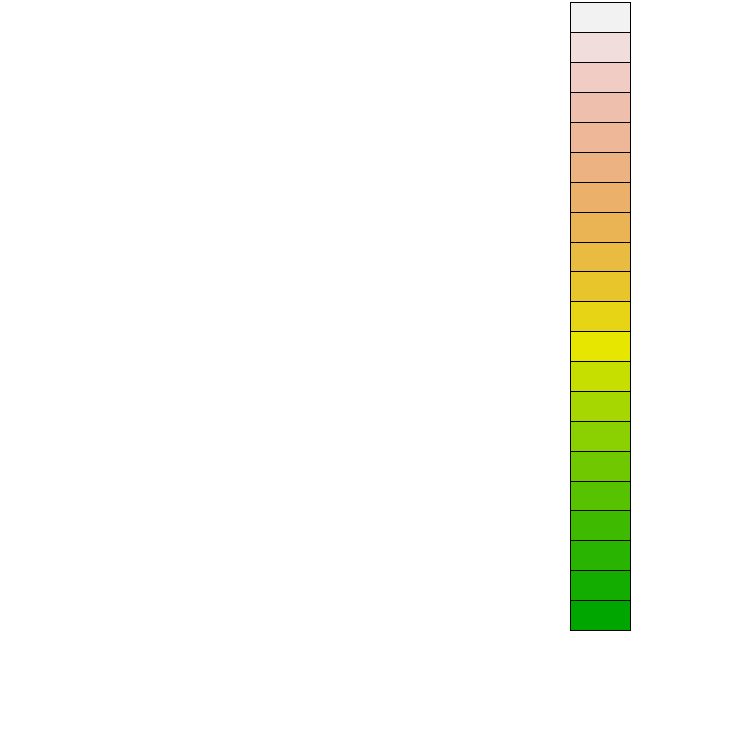
\includegraphics[width=\maxwidth]{figure/graphics-unnamed-chunk-243-1} 

}



\end{knitrout}
\caption{Linee di livello}
\label{vulcano1}
\end{center}
\end{figure}


\begin{knitrout}
\definecolor{shadecolor}{rgb}{0.969, 0.969, 0.969}\color{fgcolor}\begin{kframe}
\begin{alltt}
\hlstd{x}\hlkwb{<-} \hlkwd{c}\hlstd{(}\hlnum{0.00}\hlstd{,} \hlnum{0.40}\hlstd{,} \hlnum{0.86}\hlstd{,} \hlnum{0.85}\hlstd{,} \hlnum{0.69}\hlstd{,} \hlnum{0.48}\hlstd{,} \hlnum{0.54}\hlstd{,} \hlnum{1.09}\hlstd{,} \hlnum{1.11}\hlstd{,} \hlnum{1.73}\hlstd{,} \hlnum{2.05}\hlstd{,} \hlnum{2.02}\hlstd{)}
\hlkwd{par}\hlstd{(}\hlkwc{bg}\hlstd{=}\hlstr{"lightgray"}\hlstd{)}
\hlkwd{plot}\hlstd{(x,} \hlkwc{type}\hlstd{=}\hlstr{"n"}\hlstd{,} \hlkwc{axes}\hlstd{=}\hlnum{FALSE}\hlstd{,} \hlkwc{ann}\hlstd{=}\hlnum{FALSE}\hlstd{)}
\hlstd{usr} \hlkwb{<-} \hlkwd{par}\hlstd{(}\hlstr{"usr"}\hlstd{)}
\hlkwd{rect}\hlstd{(usr[}\hlnum{1}\hlstd{], usr[}\hlnum{3}\hlstd{], usr[}\hlnum{2}\hlstd{], usr[}\hlnum{4}\hlstd{],} \hlkwc{col}\hlstd{=}\hlstr{"cornsilk"}\hlstd{,} \hlkwc{border}\hlstd{=}\hlstr{"black"}\hlstd{)}
\hlkwd{lines}\hlstd{(x,} \hlkwc{col}\hlstd{=}\hlstr{"blue"}\hlstd{)}
\hlkwd{points}\hlstd{(x,} \hlkwc{pch}\hlstd{=}\hlnum{21}\hlstd{,} \hlkwc{bg}\hlstd{=}\hlstr{"lightcyan"}\hlstd{,} \hlkwc{cex}\hlstd{=}\hlnum{1.25}\hlstd{)}
\hlkwd{axis}\hlstd{(}\hlnum{2}\hlstd{,} \hlkwc{col.axis}\hlstd{=}\hlstr{"blue"}\hlstd{,} \hlkwc{las}\hlstd{=}\hlnum{1}\hlstd{)}
\end{alltt}


{\ttfamily\noindent\bfseries\color{errorcolor}{\#\# Error in getMetricsFromLatex(TeXMetrics, verbose = verbose): \\\#\# TeX was unable to calculate metrics for the following string\\\#\# or character:\\\#\# \\\#\# 	m\\\#\# \\\#\# Common reasons for failure include:\\\#\#\ \  * The string contains a character which is special to LaTeX unless\\\#\#\ \ \ \  escaped properly, such as \% or \$.\\\#\#\ \  * The string makes use of LaTeX commands provided by a package and\\\#\#\ \ \ \  the tikzDevice was not told to load the package.\\\#\# \\\#\# The contents of the LaTeX log of the aborted run have been printed above,\\\#\# it may contain additional details as to why the metric calculation failed.}}\begin{alltt}
\hlkwd{axis}\hlstd{(}\hlnum{1}\hlstd{,} \hlkwc{at}\hlstd{=}\hlnum{1}\hlopt{:}\hlnum{12}\hlstd{,} \hlkwc{lab}\hlstd{=month.abb,} \hlkwc{col.axis}\hlstd{=}\hlstr{"blue"}\hlstd{)}
\end{alltt}


{\ttfamily\noindent\bfseries\color{errorcolor}{\#\# Error in getMetricsFromLatex(TeXMetrics, verbose = verbose): \\\#\# TeX was unable to calculate metrics for the following string\\\#\# or character:\\\#\# \\\#\# 	m\\\#\# \\\#\# Common reasons for failure include:\\\#\#\ \  * The string contains a character which is special to LaTeX unless\\\#\#\ \ \ \  escaped properly, such as \% or \$.\\\#\#\ \  * The string makes use of LaTeX commands provided by a package and\\\#\#\ \ \ \  the tikzDevice was not told to load the package.\\\#\# \\\#\# The contents of the LaTeX log of the aborted run have been printed above,\\\#\# it may contain additional details as to why the metric calculation failed.}}\begin{alltt}
\hlkwd{box}\hlstd{()}
\hlkwd{title}\hlstd{(}\hlkwc{main}\hlstd{=}\hlstr{"Interesse per R"}\hlstd{,} \hlkwc{font.main}\hlstd{=}\hlnum{4}\hlstd{,} \hlkwc{col.main}\hlstd{=}\hlstr{"red"}\hlstd{)}
\end{alltt}


{\ttfamily\noindent\bfseries\color{errorcolor}{\#\# Error in getMetricsFromLatex(TeXMetrics, verbose = verbose): \\\#\# TeX was unable to calculate metrics for the following string\\\#\# or character:\\\#\# \\\#\# 	Interesse per R\\\#\# \\\#\# Common reasons for failure include:\\\#\#\ \  * The string contains a character which is special to LaTeX unless\\\#\#\ \ \ \  escaped properly, such as \% or \$.\\\#\#\ \  * The string makes use of LaTeX commands provided by a package and\\\#\#\ \ \ \  the tikzDevice was not told to load the package.\\\#\# \\\#\# The contents of the LaTeX log of the aborted run have been printed above,\\\#\# it may contain additional details as to why the metric calculation failed.}}\begin{alltt}
\hlkwd{title}\hlstd{(}\hlkwc{xlab}\hlstd{=}\hlstr{"1996"}\hlstd{,} \hlkwc{col.lab}\hlstd{=}\hlstr{"red"}\hlstd{)}
\end{alltt}


{\ttfamily\noindent\bfseries\color{errorcolor}{\#\# Error in getMetricsFromLatex(TeXMetrics, verbose = verbose): \\\#\# TeX was unable to calculate metrics for the following string\\\#\# or character:\\\#\# \\\#\# 	1996\\\#\# \\\#\# Common reasons for failure include:\\\#\#\ \  * The string contains a character which is special to LaTeX unless\\\#\#\ \ \ \  escaped properly, such as \% or \$.\\\#\#\ \  * The string makes use of LaTeX commands provided by a package and\\\#\#\ \ \ \  the tikzDevice was not told to load the package.\\\#\# \\\#\# The contents of the LaTeX log of the aborted run have been printed above,\\\#\# it may contain additional details as to why the metric calculation failed.}}\end{kframe}

{\centering 
\includegraphics[width=\maxwidth]{figure/graphics-unnamed-chunk-244-1} 

}



\end{knitrout}

Un esempio:

\begin{knitrout}
\definecolor{shadecolor}{rgb}{0.969, 0.969, 0.969}\color{fgcolor}\begin{kframe}
\begin{alltt}
\hlkwd{boxplot}\hlstd{(len}\hlopt{~}\hlstd{dose,} \hlkwc{data} \hlstd{= ToothGrowth,}
\hlkwc{boxwex} \hlstd{=} \hlnum{0.25}\hlstd{,} \hlkwc{at} \hlstd{=} \hlnum{1}\hlopt{:}\hlnum{3} \hlopt{-} \hlnum{0.2}\hlstd{,}
\hlkwc{subset} \hlstd{= supp} \hlopt{==} \hlstr{"VC"}\hlstd{,} \hlkwc{col} \hlstd{=} \hlstr{"yellow"}\hlstd{,}
\hlkwc{main} \hlstd{=} \hlstr{"Guinea Pigs' Tooth Growth"}\hlstd{,}
\hlkwc{xlab} \hlstd{=} \hlstr{"Vitamin C dose mg"}\hlstd{,}
\hlkwc{ylab} \hlstd{=} \hlstr{"tooth length"}\hlstd{)}
\end{alltt}


{\ttfamily\noindent\bfseries\color{errorcolor}{\#\# Error in getMetricsFromLatex(TeXMetrics, verbose = verbose): \\\#\# TeX was unable to calculate metrics for the following string\\\#\# or character:\\\#\# \\\#\# 	m\\\#\# \\\#\# Common reasons for failure include:\\\#\#\ \  * The string contains a character which is special to LaTeX unless\\\#\#\ \ \ \  escaped properly, such as \% or \$.\\\#\#\ \  * The string makes use of LaTeX commands provided by a package and\\\#\#\ \ \ \  the tikzDevice was not told to load the package.\\\#\# \\\#\# The contents of the LaTeX log of the aborted run have been printed above,\\\#\# it may contain additional details as to why the metric calculation failed.}}\end{kframe}

{\centering 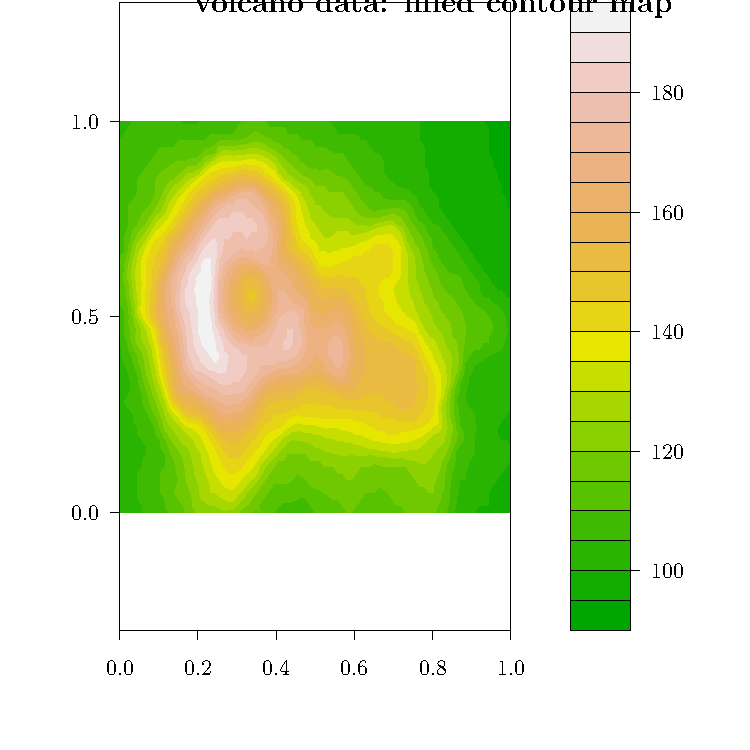
\includegraphics[width=\maxwidth]{figure/graphics-unnamed-chunk-246-1} 

}



\end{knitrout}

\subsection{I rettangoli }
\textsf{R} consente di disegnare forme (dette primitive) come rettangoli o poligoni. I rettangoli in particolare sono molto utili e versatili, consentendo di realizzare riquadri, evidenziare regioni grafiche, ecc.
%code chunk
\begin{knitrout}
\definecolor{shadecolor}{rgb}{0.969, 0.969, 0.969}\color{fgcolor}\begin{kframe}
\begin{alltt}
\hlkwd{plot}\hlstd{(}\hlkwd{c}\hlstd{(}\hlnum{100}\hlstd{,} \hlnum{200}\hlstd{),} \hlkwd{c}\hlstd{(}\hlnum{300}\hlstd{,} \hlnum{450}\hlstd{),} \hlkwc{type}\hlstd{=} \hlstr{"n"}\hlstd{,} \hlkwc{xlab}\hlstd{=}\hlstr{""}\hlstd{,} \hlkwc{ylab}\hlstd{=}\hlstr{""}\hlstd{)}
\end{alltt}


{\ttfamily\noindent\bfseries\color{errorcolor}{\#\# Error in getMetricsFromLatex(TeXMetrics, verbose = verbose): \\\#\# TeX was unable to calculate metrics for the following string\\\#\# or character:\\\#\# \\\#\# 	m\\\#\# \\\#\# Common reasons for failure include:\\\#\#\ \  * The string contains a character which is special to LaTeX unless\\\#\#\ \ \ \  escaped properly, such as \% or \$.\\\#\#\ \  * The string makes use of LaTeX commands provided by a package and\\\#\#\ \ \ \  the tikzDevice was not told to load the package.\\\#\# \\\#\# The contents of the LaTeX log of the aborted run have been printed above,\\\#\# it may contain additional details as to why the metric calculation failed.}}\begin{alltt}
\hlkwd{rect}\hlstd{(}\hlnum{100}\hlstd{,} \hlnum{300}\hlstd{,} \hlnum{125}\hlstd{,} \hlnum{350}\hlstd{)} \hlcom{# transparent}
\hlkwd{rect}\hlstd{(}\hlnum{100}\hlstd{,} \hlnum{400}\hlstd{,} \hlnum{125}\hlstd{,} \hlnum{450}\hlstd{,} \hlkwc{col}\hlstd{=}\hlstr{"green"}\hlstd{,} \hlkwc{border}\hlstd{=}\hlstr{"blue"}\hlstd{)} \hlcom{# coloured}
\hlkwd{rect}\hlstd{(}\hlnum{115}\hlstd{,} \hlnum{375}\hlstd{,} \hlnum{150}\hlstd{,} \hlnum{425}\hlstd{,} \hlkwc{col}\hlstd{=}\hlkwd{par}\hlstd{(}\hlstr{"bg"}\hlstd{),} \hlkwc{border}\hlstd{=}\hlstr{"transparent"}\hlstd{)}
\hlkwd{rect}\hlstd{(}\hlnum{150}\hlstd{,} \hlnum{300}\hlstd{,} \hlnum{175}\hlstd{,} \hlnum{350}\hlstd{,} \hlkwc{density}\hlstd{=}\hlnum{10}\hlstd{,} \hlkwc{border}\hlstd{=}\hlstr{"red"}\hlstd{)}
\hlkwd{rect}\hlstd{(}\hlnum{150}\hlstd{,} \hlnum{400}\hlstd{,} \hlnum{175}\hlstd{,} \hlnum{450}\hlstd{,} \hlkwc{density}\hlstd{=}\hlnum{30}\hlstd{,} \hlkwc{col}\hlstd{=}\hlstr{"blue"}\hlstd{,} \hlkwc{angle}\hlstd{=}\hlopt{-}\hlnum{30}\hlstd{,} \hlkwc{border}\hlstd{=}\hlstr{"transparent"}\hlstd{)}
\hlkwd{legend}\hlstd{(}\hlnum{180}\hlstd{,} \hlnum{450}\hlstd{,} \hlkwc{legend}\hlstd{=}\hlnum{1}\hlopt{:}\hlnum{4}\hlstd{,} \hlkwc{fill}\hlstd{=}\hlkwd{c}\hlstd{(}\hlnum{NA}\hlstd{,} \hlstr{"green"}\hlstd{,} \hlkwd{par}\hlstd{(}\hlstr{"fg"}\hlstd{),} \hlstr{"blue"}\hlstd{),}
\hlkwc{density}\hlstd{=}\hlkwd{c}\hlstd{(}\hlnum{NA}\hlstd{,} \hlnum{NA}\hlstd{,} \hlnum{10}\hlstd{,} \hlnum{30}\hlstd{),} \hlkwc{angle}\hlstd{=}\hlkwd{c}\hlstd{(}\hlnum{NA}\hlstd{,} \hlnum{NA}\hlstd{,} \hlnum{30}\hlstd{,} \hlopt{-}\hlnum{30}\hlstd{))}
\end{alltt}


{\ttfamily\noindent\bfseries\color{errorcolor}{\#\# Error in getMetricsFromLatex(TeXMetrics, verbose = verbose): \\\#\# TeX was unable to calculate metrics for the following string\\\#\# or character:\\\#\# \\\#\# 	1\\\#\# \\\#\# Common reasons for failure include:\\\#\#\ \  * The string contains a character which is special to LaTeX unless\\\#\#\ \ \ \  escaped properly, such as \% or \$.\\\#\#\ \  * The string makes use of LaTeX commands provided by a package and\\\#\#\ \ \ \  the tikzDevice was not told to load the package.\\\#\# \\\#\# The contents of the LaTeX log of the aborted run have been printed above,\\\#\# it may contain additional details as to why the metric calculation failed.}}\end{kframe}

{\centering 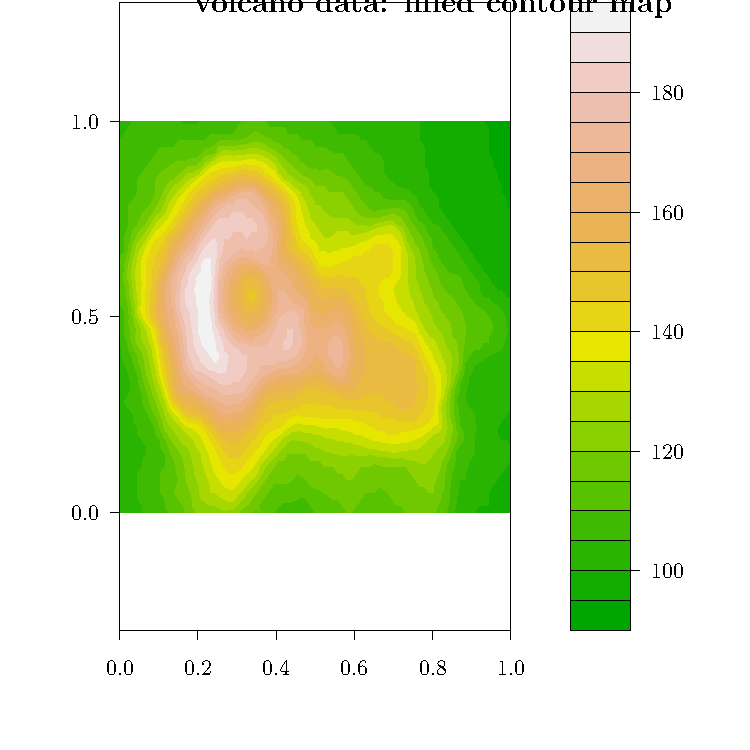
\includegraphics[width=\maxwidth]{figure/graphics-unnamed-chunk-247-1} 

}



\end{knitrout}

\section{Grafici professionali: legenda, annotazioni e formule}
Ricordiamo che una volta che sia  assegnato il livello di fiducia $1-\epsilon$, il numero $u_{1-\epsilon}$ che leggiamo nelle tabelle  distribuzione normale \`e il valore dell'ascissa tale che nell'intervallo $[-u_{1-\epsilon},u_{1-\epsilon}]$  cada un'area pari al livello di fiducia; in altre parole le 2 code della distribuzione vengono rimosse.
Vogliamo ora creare un grafico illustrativo di questa definizione.

Tracceremo inizialmente un grafico della normale tra $[-3,3]$ scegliendo come valore dell'ascissa
$u_{1-\epsilon}$  il numero  1.  Vogliamo quindi scrivere l'espressione $u_{1-\epsilon}$ nel punto di ascissa  1 e il suo opposto nel punto di ascissa -1 dell'asse $x$.
Per disegnare delle tacche sugli assi e assegnare valori alfanumerici alle stesse
si pu\`o utilizzare Il comando\selectlanguage{english}
\begin{eqnarray*}
\texttt{axis}(\varia{num},\texttt{c}(\varia{tacca}_1,\varia{tacca}_2,\ldots,\varia{tacca}_\varia{n}),\\
\texttt{c("}\varia{nome}_1, \texttt{"}\varia{nome}_2 \texttt{"},\ldots,\texttt{"}\varia{nome}_\varia{n}\texttt{"}))
\end{eqnarray*}
\selectlanguage{italian}
Qui $\varia{tacca}$ rappresenta il valore della coordinata mentre $\varia{num}$ \`e un indice che rappresenta  l'asse in esame  come segue 1=sotto, 2=sinistra, 3=sopra and 4=destra.

Possiamo  procedere con
\begin{knitrout}
\definecolor{shadecolor}{rgb}{0.969, 0.969, 0.969}\color{fgcolor}\begin{kframe}
\begin{alltt}
\hlkwd{curve}\hlstd{(}\hlkwd{dnorm}\hlstd{(x),}\hlopt{-}\hlnum{3}\hlstd{,}\hlnum{3}\hlstd{,}\hlkwc{axes}\hlstd{=}\hlnum{FALSE}\hlstd{,}\hlkwc{ylab}\hlstd{=}\hlstr{""}\hlstd{,}\hlkwc{xlab}\hlstd{=}\hlstr{""}\hlstd{,}\hlkwc{ylim}\hlstd{=}\hlkwd{c}\hlstd{(}\hlnum{0}\hlstd{,}\hlnum{0.5}\hlstd{))}
\hlkwd{axis}\hlstd{(}\hlnum{1}\hlstd{,}\hlkwd{c}\hlstd{(}\hlopt{-}\hlnum{3}\hlstd{,}\hlopt{-}\hlnum{1}\hlstd{,}\hlnum{0}\hlstd{,}\hlnum{1}\hlstd{,}\hlnum{3}\hlstd{),}\hlkwd{c}\hlstd{(}\hlstr{""}\hlstd{,}\hlkwd{expression}\hlstd{(}\hlopt{-}\hlstd{u[}\hlnum{1}\hlopt{-}\hlstd{epsilon]),}\hlnum{0}\hlstd{,}\hlkwd{expression}\hlstd{(u[}\hlnum{1}\hlopt{-}\hlstd{epsilon]),}\hlstr{""}\hlstd{))}
\end{alltt}


{\ttfamily\noindent\bfseries\color{errorcolor}{\#\# Error in getMetricsFromLatex(TeXMetrics, verbose = verbose): \\\#\# TeX was unable to calculate metrics for the following string\\\#\# or character:\\\#\# \\\#\# 	m\\\#\# \\\#\# Common reasons for failure include:\\\#\#\ \  * The string contains a character which is special to LaTeX unless\\\#\#\ \ \ \  escaped properly, such as \% or \$.\\\#\#\ \  * The string makes use of LaTeX commands provided by a package and\\\#\#\ \ \ \  the tikzDevice was not told to load the package.\\\#\# \\\#\# The contents of the LaTeX log of the aborted run have been printed above,\\\#\# it may contain additional details as to why the metric calculation failed.}}\end{kframe}
\end{knitrout}

\begin{figure}\begin{center}
\begin{knitrout}
\definecolor{shadecolor}{rgb}{0.969, 0.969, 0.969}\color{fgcolor}\begin{kframe}


{\ttfamily\noindent\bfseries\color{errorcolor}{\#\# Error in getMetricsFromLatex(TeXMetrics, verbose = verbose): \\\#\# TeX was unable to calculate metrics for the following string\\\#\# or character:\\\#\# \\\#\# 	m\\\#\# \\\#\# Common reasons for failure include:\\\#\#\ \  * The string contains a character which is special to LaTeX unless\\\#\#\ \ \ \  escaped properly, such as \% or \$.\\\#\#\ \  * The string makes use of LaTeX commands provided by a package and\\\#\#\ \ \ \  the tikzDevice was not told to load the package.\\\#\# \\\#\# The contents of the LaTeX log of the aborted run have been printed above,\\\#\# it may contain additional details as to why the metric calculation failed.}}\end{kframe}

{\centering 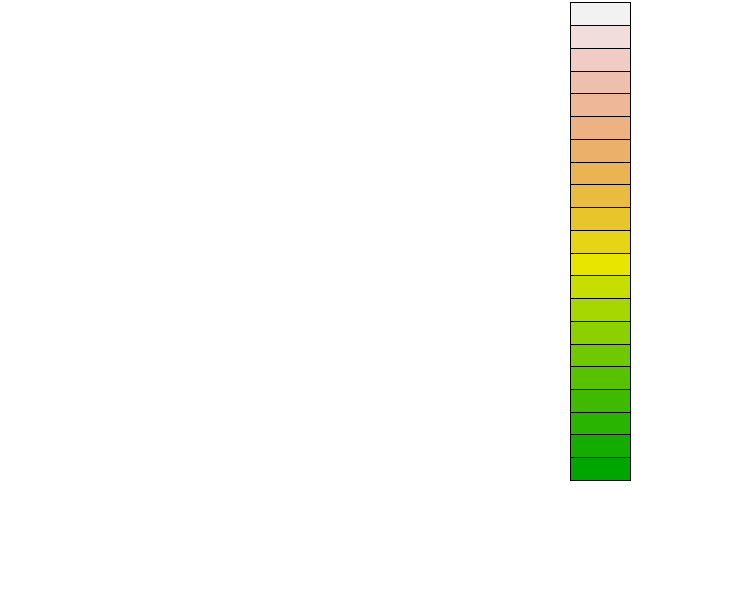
\includegraphics[width=\maxwidth]{figure/graphics-unnamed-chunk-249-1} 

}



\end{knitrout}
\caption{Selezione delle etichette sull'asse $x$. }
\label{normale13}
\end{center}
\end{figure}

Il comando \texttt{expression} consente di scrivere simboli e anche lettere greche.
Come uscita di questo primo comando troviamo il grafico~(\ref{normale13})
Per evidenziare le 2 code tratteggiamo l'area sottesa dalla normale tra 1 e 3  (e in seguito da  -3 a -1). Per operare questo tratteggio si approssima
la regione da tratteggiare con un poligono con un numero molto elevato (200) di vertici definiti come segue
%code chunk
\begin{knitrout}
\definecolor{shadecolor}{rgb}{0.969, 0.969, 0.969}\color{fgcolor}\begin{kframe}
\begin{alltt}
\hlstd{xmin}\hlkwb{<-}\hlnum{1}\hlstd{;xmax}\hlkwb{<-}\hlnum{3}\hlstd{;}
\hlstd{npunti}\hlkwb{<-}\hlnum{200}
\hlstd{f}\hlkwb{=}\hlstd{dnorm}\hlcom{#selezione degli  estremi}
\hlcom{#e del numero di punti base del poligono}
\hlstd{vals}\hlkwb{<-}\hlkwd{seq}\hlstd{(xmin,xmax,}\hlkwc{length}\hlstd{=npunti)}
\hlstd{x}\hlkwb{<-}\hlkwd{c}\hlstd{(xmin,vals,xmax,xmin)}
\hlstd{y}\hlkwb{<-}\hlkwd{c}\hlstd{(}\hlnum{0}\hlstd{,}\hlkwd{f}\hlstd{(vals),}\hlnum{0}\hlstd{,}\hlnum{0}\hlstd{);}
\end{alltt}
\end{kframe}
\end{knitrout}

La sintassi di \texttt{polygon}?\`e
\begin{eqnarray*}
\texttt{polygon}(\varia{x,y},\texttt{density}=\varia{val1},
\texttt{angle}=\varia{val2},
\\
\texttt{col=\virgolette col\virgolette
})
\end{eqnarray*}

Il comando
\begin{knitrout}
\definecolor{shadecolor}{rgb}{0.969, 0.969, 0.969}\color{fgcolor}\begin{kframe}
\begin{alltt}
\hlkwd{curve}\hlstd{(}\hlkwd{dnorm}\hlstd{(x),}\hlopt{-}\hlnum{3}\hlstd{,}\hlnum{3}\hlstd{,}\hlkwc{axes}\hlstd{=}\hlnum{FALSE}\hlstd{,}\hlkwc{ylab}\hlstd{=}\hlstr{""}\hlstd{,}\hlkwc{xlab}\hlstd{=}\hlstr{""}\hlstd{,}\hlkwc{ylim}\hlstd{=}\hlkwd{c}\hlstd{(}\hlnum{0}\hlstd{,}\hlnum{0.5}\hlstd{))}
\hlkwd{axis}\hlstd{(}\hlnum{1}\hlstd{,}\hlkwd{c}\hlstd{(}\hlopt{-}\hlnum{3}\hlstd{,}\hlopt{-}\hlnum{1}\hlstd{,}\hlnum{0}\hlstd{,}\hlnum{1}\hlstd{,}\hlnum{3}\hlstd{),}\hlkwd{c}\hlstd{(}\hlstr{""}\hlstd{,}\hlkwd{expression}\hlstd{(}\hlopt{-}\hlstd{u[}\hlnum{1}\hlopt{-}\hlstd{epsilon]),}\hlnum{0}\hlstd{,}\hlkwd{expression}\hlstd{(u[}\hlnum{1}\hlopt{-}\hlstd{epsilon]),}\hlstr{""}\hlstd{))}
\end{alltt}


{\ttfamily\noindent\bfseries\color{errorcolor}{\#\# Error in getMetricsFromLatex(TeXMetrics, verbose = verbose): \\\#\# TeX was unable to calculate metrics for the following string\\\#\# or character:\\\#\# \\\#\# 	m\\\#\# \\\#\# Common reasons for failure include:\\\#\#\ \  * The string contains a character which is special to LaTeX unless\\\#\#\ \ \ \  escaped properly, such as \% or \$.\\\#\#\ \  * The string makes use of LaTeX commands provided by a package and\\\#\#\ \ \ \  the tikzDevice was not told to load the package.\\\#\# \\\#\# The contents of the LaTeX log of the aborted run have been printed above,\\\#\# it may contain additional details as to why the metric calculation failed.}}\begin{alltt}
\hlkwd{points}\hlstd{(x,y,}\hlkwc{pch}\hlstd{=}\hlnum{20}\hlstd{,}\hlkwc{col}\hlstd{=}\hlstr{"red"}\hlstd{,}\hlkwc{cex}\hlstd{=}\hlnum{0.2}\hlstd{)}
\end{alltt}
\end{kframe}
\end{knitrout}
consente la visualizzazione dei punti ottenuti (come in figura~(\ref{normale200punti})).

\begin{figure}\begin{center}
\begin{knitrout}
\definecolor{shadecolor}{rgb}{0.969, 0.969, 0.969}\color{fgcolor}\begin{kframe}


{\ttfamily\noindent\bfseries\color{errorcolor}{\#\# Error in getMetricsFromLatex(TeXMetrics, verbose = verbose): \\\#\# TeX was unable to calculate metrics for the following string\\\#\# or character:\\\#\# \\\#\# 	m\\\#\# \\\#\# Common reasons for failure include:\\\#\#\ \  * The string contains a character which is special to LaTeX unless\\\#\#\ \ \ \  escaped properly, such as \% or \$.\\\#\#\ \  * The string makes use of LaTeX commands provided by a package and\\\#\#\ \ \ \  the tikzDevice was not told to load the package.\\\#\# \\\#\# The contents of the LaTeX log of the aborted run have been printed above,\\\#\# it may contain additional details as to why the metric calculation failed.}}\end{kframe}

{\centering 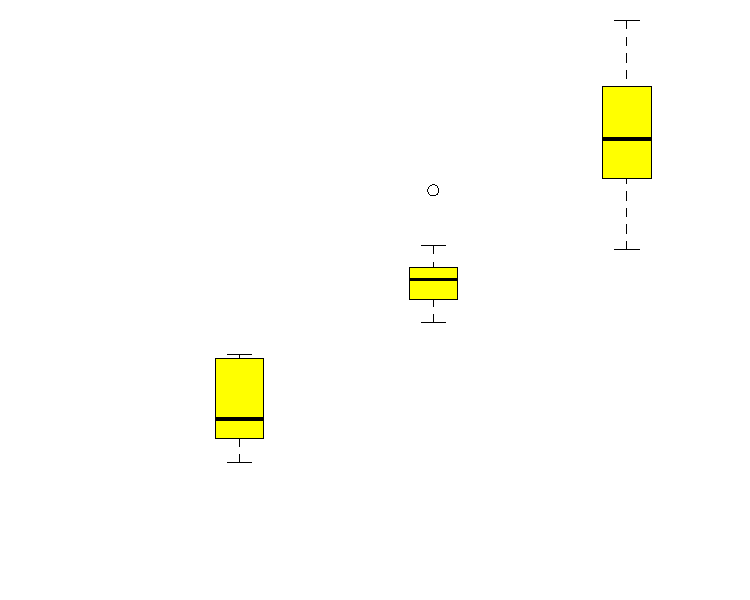
\includegraphics[width=\maxwidth]{figure/graphics-unnamed-chunk-252-1} 

}



\end{knitrout}
\caption{ Selezione dei punti per l'ombreggiamento di una regione poligonale}
\label{normale200punti}
\end{center}
\end{figure}

Questi punti  possono poi essere uniti con una curva poligonale
\begin{knitrout}
\definecolor{shadecolor}{rgb}{0.969, 0.969, 0.969}\color{fgcolor}\begin{kframe}
\begin{alltt}
\hlkwd{curve}\hlstd{(}\hlkwd{dnorm}\hlstd{(x),}\hlopt{-}\hlnum{3}\hlstd{,}\hlnum{3}\hlstd{,}\hlkwc{axes}\hlstd{=}\hlnum{FALSE}\hlstd{,}\hlkwc{ylab}\hlstd{=}\hlstr{""}\hlstd{,}\hlkwc{xlab}\hlstd{=}\hlstr{""}\hlstd{,}\hlkwc{ylim}\hlstd{=}\hlkwd{c}\hlstd{(}\hlnum{0}\hlstd{,}\hlnum{0.5}\hlstd{))}
\hlkwd{axis}\hlstd{(}\hlnum{1}\hlstd{,}\hlkwd{c}\hlstd{(}\hlopt{-}\hlnum{3}\hlstd{,}\hlopt{-}\hlnum{1}\hlstd{,}\hlnum{0}\hlstd{,}\hlnum{1}\hlstd{,}\hlnum{3}\hlstd{),}\hlkwd{c}\hlstd{(}\hlstr{""}\hlstd{,}\hlkwd{expression}\hlstd{(}\hlopt{-}\hlstd{u[}\hlnum{1}\hlopt{-}\hlstd{epsilon]),}\hlnum{0}\hlstd{,}\hlkwd{expression}\hlstd{(u[}\hlnum{1}\hlopt{-}\hlstd{epsilon]),}\hlstr{""}\hlstd{))}
\end{alltt}


{\ttfamily\noindent\bfseries\color{errorcolor}{\#\# Error in getMetricsFromLatex(TeXMetrics, verbose = verbose): \\\#\# TeX was unable to calculate metrics for the following string\\\#\# or character:\\\#\# \\\#\# 	m\\\#\# \\\#\# Common reasons for failure include:\\\#\#\ \  * The string contains a character which is special to LaTeX unless\\\#\#\ \ \ \  escaped properly, such as \% or \$.\\\#\#\ \  * The string makes use of LaTeX commands provided by a package and\\\#\#\ \ \ \  the tikzDevice was not told to load the package.\\\#\# \\\#\# The contents of the LaTeX log of the aborted run have been printed above,\\\#\# it may contain additional details as to why the metric calculation failed.}}\begin{alltt}
\hlkwd{points}\hlstd{(x,y,}\hlkwc{pch}\hlstd{=}\hlnum{20}\hlstd{,}\hlkwc{col}\hlstd{=}\hlstr{"red"}\hlstd{,}\hlkwc{cex}\hlstd{=}\hlnum{0.2}\hlstd{)}
\hlkwd{polygon}\hlstd{(x,y,}\hlkwc{density}\hlstd{=}\hlnum{20}\hlstd{,}\hlkwc{angle}\hlstd{=}\hlnum{45}\hlstd{,}\hlkwc{col}\hlstd{=}\hlstr{"RED"}\hlstd{)}
\hlstd{x}\hlkwb{<-}\hlopt{-}\hlstd{x}
\hlstd{y}\hlkwb{<-}\hlkwd{c}\hlstd{(}\hlnum{0}\hlstd{,}\hlkwd{dnorm}\hlstd{(}\hlopt{-}\hlstd{vals),}\hlnum{0}\hlstd{,}\hlnum{0}\hlstd{)}
\hlkwd{polygon}\hlstd{(x,y,}\hlkwc{density}\hlstd{=}\hlnum{20}\hlstd{,}\hlkwc{angle}\hlstd{=}\hlnum{45}\hlstd{,}\hlkwc{col}\hlstd{=}\hlstr{"RED"}\hlstd{)}
\end{alltt}
\end{kframe}

{\centering 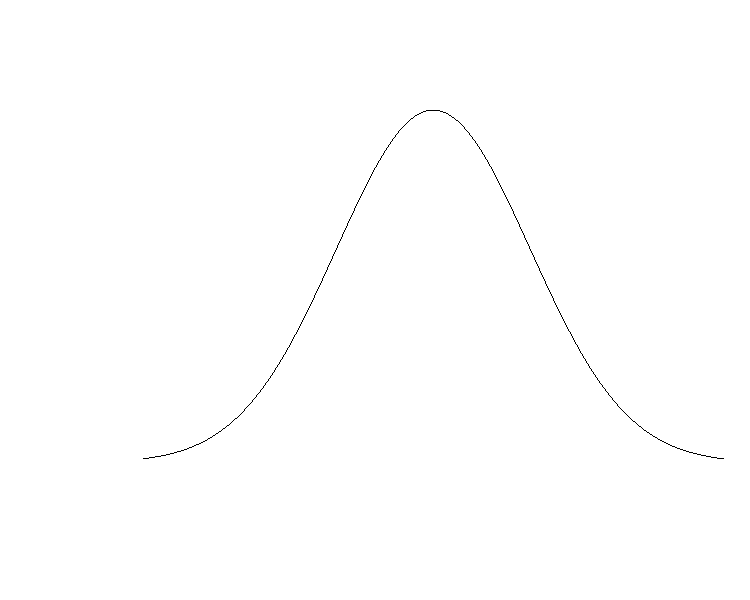
\includegraphics[width=\maxwidth]{figure/graphics-a-1} 

}



\end{knitrout}

Infine possiamo riportare i valori delle aree delle 2 code, evidenziare l'asse di simmetria  e dare un titolo al grafico


\begin{knitrout}
\definecolor{shadecolor}{rgb}{0.969, 0.969, 0.969}\color{fgcolor}\begin{kframe}
\begin{alltt}
\hlkwd{curve}\hlstd{(}\hlkwd{dnorm}\hlstd{(x),}\hlopt{-}\hlnum{3}\hlstd{,}\hlnum{3}\hlstd{,}\hlkwc{axes}\hlstd{=}\hlnum{FALSE}\hlstd{,}\hlkwc{ylab}\hlstd{=}\hlstr{""}\hlstd{,}\hlkwc{xlab}\hlstd{=}\hlstr{""}\hlstd{,}\hlkwc{ylim}\hlstd{=}\hlkwd{c}\hlstd{(}\hlnum{0}\hlstd{,}\hlnum{0.5}\hlstd{))}
\hlkwd{axis}\hlstd{(}\hlnum{1}\hlstd{,}\hlkwd{c}\hlstd{(}\hlopt{-}\hlnum{3}\hlstd{,}\hlopt{-}\hlnum{1}\hlstd{,}\hlnum{0}\hlstd{,}\hlnum{1}\hlstd{,}\hlnum{3}\hlstd{),}\hlkwd{c}\hlstd{(}\hlstr{""}\hlstd{,}\hlkwd{expression}\hlstd{(}\hlopt{-}\hlstd{u[}\hlnum{1}\hlopt{-}\hlstd{epsilon]),}\hlnum{0}\hlstd{,}\hlkwd{expression}\hlstd{(u[}\hlnum{1}\hlopt{-}\hlstd{epsilon]),}\hlstr{""}\hlstd{))}
\end{alltt}


{\ttfamily\noindent\bfseries\color{errorcolor}{\#\# Error in getMetricsFromLatex(TeXMetrics, verbose = verbose): \\\#\# TeX was unable to calculate metrics for the following string\\\#\# or character:\\\#\# \\\#\# 	m\\\#\# \\\#\# Common reasons for failure include:\\\#\#\ \  * The string contains a character which is special to LaTeX unless\\\#\#\ \ \ \  escaped properly, such as \% or \$.\\\#\#\ \  * The string makes use of LaTeX commands provided by a package and\\\#\#\ \ \ \  the tikzDevice was not told to load the package.\\\#\# \\\#\# The contents of the LaTeX log of the aborted run have been printed above,\\\#\# it may contain additional details as to why the metric calculation failed.}}\begin{alltt}
\hlkwd{points}\hlstd{(x,y,}\hlkwc{pch}\hlstd{=}\hlnum{20}\hlstd{,}\hlkwc{col}\hlstd{=}\hlstr{"red"}\hlstd{,}\hlkwc{cex}\hlstd{=}\hlnum{0.2}\hlstd{)}
\hlkwd{polygon}\hlstd{(x,y,}\hlkwc{density}\hlstd{=}\hlnum{20}\hlstd{,}\hlkwc{angle}\hlstd{=}\hlnum{45}\hlstd{,}\hlkwc{col}\hlstd{=}\hlstr{"RED"}\hlstd{)}
\hlstd{x}\hlkwb{<-}\hlopt{-}\hlstd{x}
\hlstd{y}\hlkwb{<-}\hlkwd{c}\hlstd{(}\hlnum{0}\hlstd{,}\hlkwd{dnorm}\hlstd{(}\hlopt{-}\hlstd{vals),}\hlnum{0}\hlstd{,}\hlnum{0}\hlstd{)}
\hlkwd{polygon}\hlstd{(x,y,}\hlkwc{density}\hlstd{=}\hlnum{20}\hlstd{,}\hlkwc{angle}\hlstd{=}\hlnum{45}\hlstd{,}\hlkwc{col}\hlstd{=}\hlstr{"RED"}\hlstd{)}
\hlkwd{polygon}\hlstd{(x,y,}\hlkwc{density}\hlstd{=}\hlnum{20}\hlstd{,}\hlkwc{angle}\hlstd{=}\hlnum{45}\hlstd{,}\hlkwc{col}\hlstd{=}\hlstr{"RED"}\hlstd{)}
\hlkwd{abline}\hlstd{(}\hlkwc{h}\hlstd{=}\hlkwd{min}\hlstd{(y))}
\hlkwd{text}\hlstd{(}\hlnum{0}\hlstd{,}\hlnum{0.45}\hlstd{,}\hlkwd{expression}\hlstd{(}\hlstr{"code della gaussiana"}\hlstd{))}
\end{alltt}


{\ttfamily\noindent\bfseries\color{errorcolor}{\#\# Error in getMetricsFromLatex(TeXMetrics, verbose = verbose): \\\#\# TeX was unable to calculate metrics for the following string\\\#\# or character:\\\#\# \\\#\# 	77\\\#\# \\\#\# Common reasons for failure include:\\\#\#\ \  * The string contains a character which is special to LaTeX unless\\\#\#\ \ \ \  escaped properly, such as \% or \$.\\\#\#\ \  * The string makes use of LaTeX commands provided by a package and\\\#\#\ \ \ \  the tikzDevice was not told to load the package.\\\#\# \\\#\# The contents of the LaTeX log of the aborted run have been printed above,\\\#\# it may contain additional details as to why the metric calculation failed.}}\begin{alltt}
\hlkwd{text}\hlstd{(}\hlopt{-}\hlnum{1.6}\hlstd{,}\hlnum{0.03}\hlstd{,}\hlkwd{expression}\hlstd{(epsilon}\hlopt{/}\hlnum{2}\hlstd{))}
\end{alltt}


{\ttfamily\noindent\bfseries\color{errorcolor}{\#\# Error in getMetricsFromLatex(TeXMetrics, verbose = verbose): \\\#\# TeX was unable to calculate metrics for the following string\\\#\# or character:\\\#\# \\\#\# 	77\\\#\# \\\#\# Common reasons for failure include:\\\#\#\ \  * The string contains a character which is special to LaTeX unless\\\#\#\ \ \ \  escaped properly, such as \% or \$.\\\#\#\ \  * The string makes use of LaTeX commands provided by a package and\\\#\#\ \ \ \  the tikzDevice was not told to load the package.\\\#\# \\\#\# The contents of the LaTeX log of the aborted run have been printed above,\\\#\# it may contain additional details as to why the metric calculation failed.}}\begin{alltt}
\hlkwd{text}\hlstd{(}\hlnum{1.6}\hlstd{,}\hlnum{0.03}\hlstd{,}\hlkwd{expression}\hlstd{(epsilon}\hlopt{/}\hlnum{2}\hlstd{))}
\end{alltt}


{\ttfamily\noindent\bfseries\color{errorcolor}{\#\# Error in getMetricsFromLatex(TeXMetrics, verbose = verbose): \\\#\# TeX was unable to calculate metrics for the following string\\\#\# or character:\\\#\# \\\#\# 	77\\\#\# \\\#\# Common reasons for failure include:\\\#\#\ \  * The string contains a character which is special to LaTeX unless\\\#\#\ \ \ \  escaped properly, such as \% or \$.\\\#\#\ \  * The string makes use of LaTeX commands provided by a package and\\\#\#\ \ \ \  the tikzDevice was not told to load the package.\\\#\# \\\#\# The contents of the LaTeX log of the aborted run have been printed above,\\\#\# it may contain additional details as to why the metric calculation failed.}}\begin{alltt}
\hlkwd{lines}\hlstd{(}\hlkwd{c}\hlstd{(}\hlnum{0}\hlstd{,}\hlnum{0}\hlstd{),}\hlkwd{c}\hlstd{(}\hlnum{0}\hlstd{,}\hlkwd{dnorm}\hlstd{(}\hlnum{0}\hlstd{)))}
\end{alltt}
\end{kframe}

{\centering 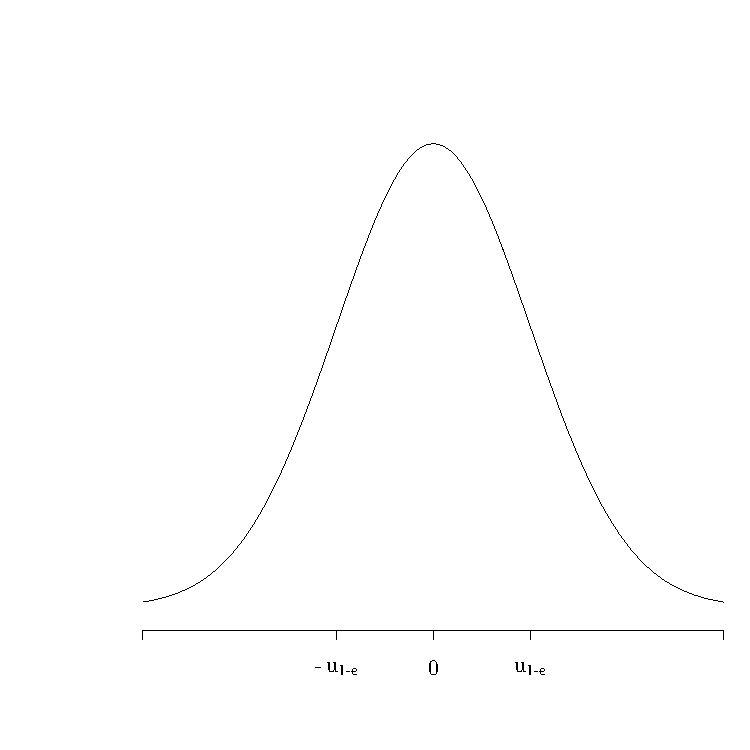
\includegraphics[width=\maxwidth]{figure/graphics-unnamed-chunk-253-1} 

}



\end{knitrout}

\begin{figure}\begin{center}
\begin{knitrout}
\definecolor{shadecolor}{rgb}{0.969, 0.969, 0.969}\color{fgcolor}\begin{kframe}
\begin{alltt}
\hlkwd{curve}\hlstd{(}\hlkwd{dnorm}\hlstd{(x),}\hlopt{-}\hlnum{3}\hlstd{,}\hlnum{3}\hlstd{,}\hlkwc{axes}\hlstd{=}\hlnum{FALSE}\hlstd{,}\hlkwc{ylab}\hlstd{=}\hlstr{""}\hlstd{,}\hlkwc{xlab}\hlstd{=}\hlstr{""}\hlstd{,}\hlkwc{ylim}\hlstd{=}\hlkwd{c}\hlstd{(}\hlnum{0}\hlstd{,}\hlnum{0.5}\hlstd{))}
\hlkwd{polygon}\hlstd{(x,y,}\hlkwc{density}\hlstd{=}\hlnum{20}\hlstd{,}\hlkwc{angle}\hlstd{=}\hlnum{45}\hlstd{,}\hlkwc{col}\hlstd{=}\hlstr{"RED"}\hlstd{)}
\hlkwd{abline}\hlstd{(}\hlkwc{h}\hlstd{=}\hlkwd{min}\hlstd{(y))}
\hlkwd{text}\hlstd{(}\hlnum{0}\hlstd{,}\hlnum{0.45}\hlstd{,}\hlkwd{expression}\hlstd{(}\hlstr{"code della gaussiana"}\hlstd{))}
\end{alltt}


{\ttfamily\noindent\bfseries\color{errorcolor}{\#\# Error in getMetricsFromLatex(TeXMetrics, verbose = verbose): \\\#\# TeX was unable to calculate metrics for the following string\\\#\# or character:\\\#\# \\\#\# 	77\\\#\# \\\#\# Common reasons for failure include:\\\#\#\ \  * The string contains a character which is special to LaTeX unless\\\#\#\ \ \ \  escaped properly, such as \% or \$.\\\#\#\ \  * The string makes use of LaTeX commands provided by a package and\\\#\#\ \ \ \  the tikzDevice was not told to load the package.\\\#\# \\\#\# The contents of the LaTeX log of the aborted run have been printed above,\\\#\# it may contain additional details as to why the metric calculation failed.}}\begin{alltt}
\hlkwd{text}\hlstd{(}\hlopt{-}\hlnum{1.6}\hlstd{,}\hlnum{0.03}\hlstd{,}\hlkwd{expression}\hlstd{(epsilon}\hlopt{/}\hlnum{2}\hlstd{))}
\end{alltt}


{\ttfamily\noindent\bfseries\color{errorcolor}{\#\# Error in getMetricsFromLatex(TeXMetrics, verbose = verbose): \\\#\# TeX was unable to calculate metrics for the following string\\\#\# or character:\\\#\# \\\#\# 	77\\\#\# \\\#\# Common reasons for failure include:\\\#\#\ \  * The string contains a character which is special to LaTeX unless\\\#\#\ \ \ \  escaped properly, such as \% or \$.\\\#\#\ \  * The string makes use of LaTeX commands provided by a package and\\\#\#\ \ \ \  the tikzDevice was not told to load the package.\\\#\# \\\#\# The contents of the LaTeX log of the aborted run have been printed above,\\\#\# it may contain additional details as to why the metric calculation failed.}}\begin{alltt}
\hlkwd{text}\hlstd{(}\hlnum{1.6}\hlstd{,}\hlnum{0.03}\hlstd{,}\hlkwd{expression}\hlstd{(epsilon}\hlopt{/}\hlnum{2}\hlstd{))}
\end{alltt}


{\ttfamily\noindent\bfseries\color{errorcolor}{\#\# Error in getMetricsFromLatex(TeXMetrics, verbose = verbose): \\\#\# TeX was unable to calculate metrics for the following string\\\#\# or character:\\\#\# \\\#\# 	77\\\#\# \\\#\# Common reasons for failure include:\\\#\#\ \  * The string contains a character which is special to LaTeX unless\\\#\#\ \ \ \  escaped properly, such as \% or \$.\\\#\#\ \  * The string makes use of LaTeX commands provided by a package and\\\#\#\ \ \ \  the tikzDevice was not told to load the package.\\\#\# \\\#\# The contents of the LaTeX log of the aborted run have been printed above,\\\#\# it may contain additional details as to why the metric calculation failed.}}\begin{alltt}
\hlkwd{lines}\hlstd{(}\hlkwd{c}\hlstd{(}\hlnum{0}\hlstd{,}\hlnum{0}\hlstd{),}\hlkwd{c}\hlstd{(}\hlnum{0}\hlstd{,}\hlkwd{dnorm}\hlstd{(}\hlnum{0}\hlstd{)))}
\end{alltt}
\end{kframe}

{\centering 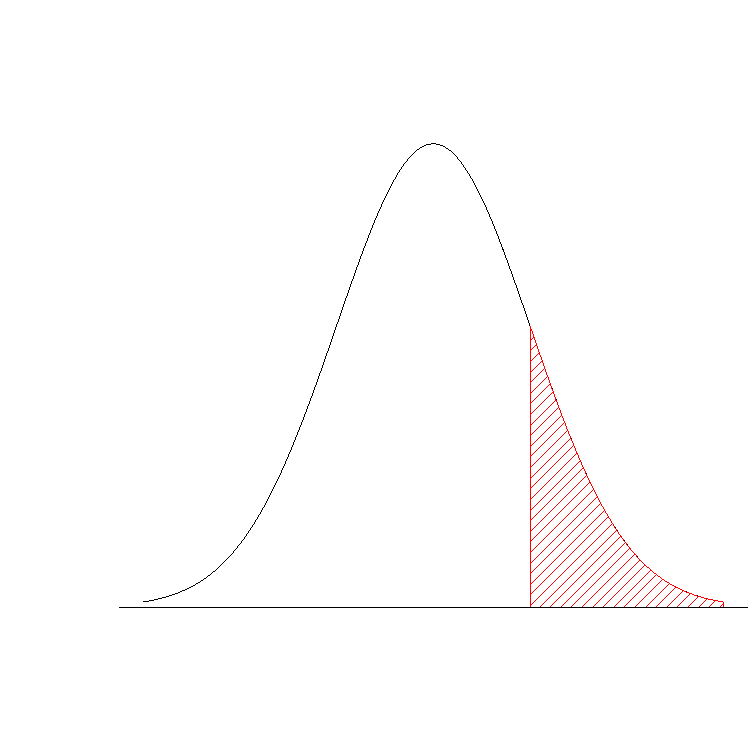
\includegraphics[width=\maxwidth]{figure/graphics-unnamed-chunk-254-1} 

}



\end{knitrout}
\caption{ Area delle code della distribuzione normale. Il valore di $u_{1-\epsilon}$ \`e quello riportato nella  tabella della distribuzione normale. }
\label{normaletratto}
\end{center}
\end{figure}

\section{Pittura virtuale}
Iniziamo a disegnare dei rettangoli, di coordinate casuali ma entro un dato range, di colore casuale, con spessore del bordo casuale.
\begin{knitrout}
\definecolor{shadecolor}{rgb}{0.969, 0.969, 0.969}\color{fgcolor}\begin{kframe}
\begin{alltt}
\hlkwd{par}\hlstd{(}\hlkwc{bg}\hlstd{=}\hlstr{"skyblue"}\hlstd{);}
\hlkwd{plot}\hlstd{(}\hlnum{0}\hlstd{,}\hlkwc{xlim}\hlstd{=}\hlkwd{c}\hlstd{(}\hlnum{0.3}\hlstd{,}\hlnum{1}\hlstd{),}\hlkwc{ylim}\hlstd{=}\hlkwd{c}\hlstd{(}\hlnum{0.3}\hlstd{,}\hlnum{1}\hlstd{),}\hlkwc{axes}\hlstd{=F,} \hlkwc{xlab}\hlstd{=}\hlstr{""}\hlstd{,}\hlkwc{ylab}\hlstd{=}\hlstr{""}\hlstd{)}
\hlkwa{for}\hlstd{(i} \hlkwa{in} \hlnum{1}\hlopt{:}\hlnum{100}\hlstd{)}
\hlstd{\{} \hlkwd{Sys.sleep}\hlstd{(}\hlnum{0.01}\hlstd{);}
\hlkwd{runif}\hlstd{(}\hlnum{1}\hlstd{)}\hlkwb{->}\hlstd{sotto;}
\hlkwd{runif}\hlstd{(}\hlnum{1}\hlstd{)}\hlkwb{->}\hlstd{sinistra;}
\hlkwd{runif}\hlstd{(}\hlnum{1}\hlstd{)}\hlopt{+}\hlstd{sotto}\hlkwb{->}\hlstd{sopra;}
\hlkwd{runif}\hlstd{(}\hlnum{1}\hlstd{)}\hlopt{+}\hlstd{sinistra}\hlkwb{->}\hlstd{destra;}
\hlstd{bordi}\hlkwb{<-}\hlnum{0}\hlstd{;}\hlkwa{for}\hlstd{(i} \hlkwa{in} \hlnum{1}\hlopt{:}\hlnum{100}\hlstd{) bordi[i]}\hlkwb{<-}\hlkwd{floor}\hlstd{(}\hlkwd{runif}\hlstd{(}\hlnum{1}\hlstd{,}\hlnum{1}\hlstd{,}\hlnum{10}\hlstd{))}
\hlstd{spess}\hlkwb{<-}\hlnum{0}\hlstd{;}\hlkwa{for}\hlstd{(i} \hlkwa{in} \hlnum{1}\hlopt{:}\hlnum{100}\hlstd{) spess[i]}\hlkwb{<-}\hlkwd{floor}\hlstd{(}\hlkwd{runif}\hlstd{(}\hlnum{1}\hlstd{,}\hlnum{1}\hlstd{,}\hlnum{10}\hlstd{))}
\hlkwd{rect}\hlstd{(sinistra,sotto,destra,sopra,}\hlkwc{col}\hlstd{=}\hlkwd{rgb}\hlstd{(}\hlkwd{runif}\hlstd{(}\hlnum{1}\hlstd{),}\hlkwd{runif}\hlstd{(}\hlnum{1}\hlstd{),}\hlkwd{runif}\hlstd{(}\hlnum{1}\hlstd{)),}\hlkwc{border}\hlstd{=bordi[i],}\hlkwc{lwd}\hlstd{=spess)\}}
\end{alltt}
\end{kframe}

{\centering 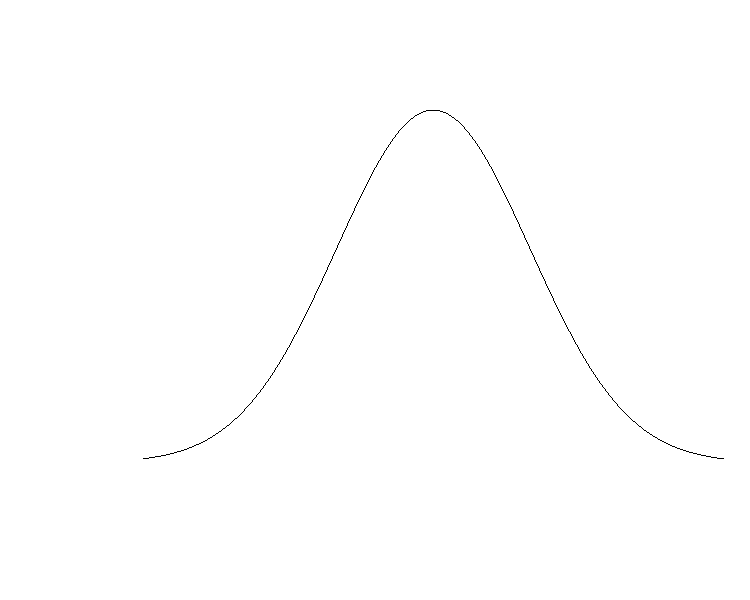
\includegraphics[width=\maxwidth]{figure/graphics-unnamed-chunk-255-1} 

}



\end{knitrout}
\section{Grafica 3D, il vulcano Maunga Whau}
Con il codice che segue

\begin{knitrout}
\definecolor{shadecolor}{rgb}{0.969, 0.969, 0.969}\color{fgcolor}\begin{kframe}
\begin{alltt}
\hlstd{z}\hlkwb{<-} \hlnum{2} \hlopt{*} \hlstd{volcano}
\hlstd{x}\hlkwb{<-} \hlnum{10} \hlopt{*} \hlstd{(}\hlnum{1}\hlopt{:}\hlkwd{nrow}\hlstd{(z))}
\hlstd{y}\hlkwb{<-} \hlnum{10} \hlopt{*} \hlstd{(}\hlnum{1}\hlopt{:}\hlkwd{ncol}\hlstd{(z))}
\hlstd{z0}\hlkwb{<-} \hlkwd{min}\hlstd{(z)} \hlopt{-} \hlnum{20}
\hlstd{z}\hlkwb{<-} \hlkwd{rbind}\hlstd{(z0,} \hlkwd{cbind}\hlstd{(z0, z, z0), z0)}
\hlstd{x}\hlkwb{<-} \hlkwd{c}\hlstd{(}\hlkwd{min}\hlstd{(x)} \hlopt{-} \hlnum{1e-10}\hlstd{, x,} \hlkwd{max}\hlstd{(x)} \hlopt{+} \hlnum{1e-10}\hlstd{)}
\hlstd{y}\hlkwb{<-} \hlkwd{c}\hlstd{(}\hlkwd{min}\hlstd{(y)} \hlopt{-} \hlnum{1e-10}\hlstd{, y,} \hlkwd{max}\hlstd{(y)} \hlopt{+} \hlnum{1e-10}\hlstd{)}
\hlstd{fill} \hlkwb{<-} \hlkwd{matrix}\hlstd{(}\hlstr{"green3"}\hlstd{,} \hlkwc{nr} \hlstd{=} \hlkwd{nrow}\hlstd{(z)}\hlopt{-}\hlnum{1}\hlstd{,} \hlkwc{nc} \hlstd{=} \hlkwd{ncol}\hlstd{(z)}\hlopt{-}\hlnum{1}\hlstd{)}
\hlstd{fill[ , i2} \hlkwb{<-} \hlkwd{c}\hlstd{(}\hlnum{1}\hlstd{,}\hlkwd{ncol}\hlstd{(fill))]} \hlkwb{<-} \hlstr{"gray"}
\hlstd{fill[i1} \hlkwb{<-} \hlkwd{c}\hlstd{(}\hlnum{1}\hlstd{,}\hlkwd{nrow}\hlstd{(fill)) , ]} \hlkwb{<-} \hlstr{"gray"}
\hlstd{fcol} \hlkwb{<-} \hlstd{fill}
\hlstd{zi} \hlkwb{<-} \hlstd{volcano[} \hlopt{-}\hlnum{1}\hlstd{,}\hlopt{-}\hlnum{1}\hlstd{]} \hlopt{+} \hlstd{volcano[} \hlopt{-}\hlnum{1}\hlstd{,}\hlopt{-}\hlnum{61}\hlstd{]} \hlopt{+}
\hlstd{volcano[}\hlopt{-}\hlnum{87}\hlstd{,}\hlopt{-}\hlnum{1}\hlstd{]} \hlopt{+} \hlstd{volcano[}\hlopt{-}\hlnum{87}\hlstd{,}\hlopt{-}\hlnum{61}\hlstd{]} \hlcom{## / 4}
\hlstd{fcol[}\hlopt{-}\hlstd{i1,}\hlopt{-}\hlstd{i2]} \hlkwb{<-} \hlkwd{terrain.colors}\hlstd{(}\hlnum{20}\hlstd{)[}\hlkwd{cut}\hlstd{(zi,} \hlkwd{quantile}\hlstd{(zi,} \hlkwd{seq}\hlstd{(}\hlnum{0}\hlstd{,}\hlnum{1}\hlstd{,} \hlkwc{len} \hlstd{=} \hlnum{21}\hlstd{)),}
\hlkwc{include.lowest} \hlstd{=} \hlnum{TRUE}\hlstd{)]}
\hlkwd{par}\hlstd{(}\hlkwc{mar}\hlstd{=}\hlkwd{rep}\hlstd{(}\hlnum{.5}\hlstd{,}\hlnum{4}\hlstd{))}
\hlkwd{persp}\hlstd{(x, y,} \hlnum{2}\hlopt{*}\hlstd{z,} \hlkwc{theta} \hlstd{=} \hlnum{110}\hlstd{,} \hlkwc{phi} \hlstd{=} \hlnum{40}\hlstd{,} \hlkwc{col} \hlstd{= fcol,} \hlkwc{scale} \hlstd{=} \hlnum{FALSE}\hlstd{,}
\hlkwc{ltheta} \hlstd{=} \hlopt{-}\hlnum{120}\hlstd{,} \hlkwc{shade} \hlstd{=} \hlnum{0.4}\hlstd{,} \hlkwc{border} \hlstd{=} \hlnum{NA}\hlstd{,} \hlkwc{box} \hlstd{=} \hlnum{FALSE}\hlstd{)}
\end{alltt}
\end{kframe}
\end{knitrout}
otteniamo la figura~\ref{vulcano3D}. Il comando di base \`e \texttt{persp} che richiede una griglia di valori di $(x,y)$ e il corrispondente valore di quota.
\begin{figure}[htbp]
\begin{center}
\begin{knitrout}
\definecolor{shadecolor}{rgb}{0.969, 0.969, 0.969}\color{fgcolor}

{\centering \includegraphics[width=\maxwidth]{figure/graphics-unnamed-chunk-257-1} 

}



\end{knitrout}

\caption{Grafica 3 dimensionale, ottenuta con il comando \texttt{persp}}
\label{vulcano3D}
\end{center}
\end{figure}

 Costruiamo due curve che rappresentano due distribuzioni normali, in particolare al posto della funzione \texttt{dnorm} andremo a calcolare i singoli valori di $y$ associati ad un set di valori di
$x$, essendo poi liberi di utilizzare la funzione \texttt{plot}


\begin{knitrout}
\definecolor{shadecolor}{rgb}{0.969, 0.969, 0.969}\color{fgcolor}\begin{kframe}
\begin{alltt}
\hlkwd{options}\hlstd{(}\hlkwc{width}\hlstd{=}\hlnum{60}\hlstd{)}
\hlstd{x}\hlkwb{<-}\hlkwd{seq}\hlstd{(}\hlopt{-}\hlnum{10}\hlstd{,}\hlnum{10}\hlstd{,}\hlkwc{length}\hlstd{=}\hlnum{400}\hlstd{)}
\hlstd{y1}\hlkwb{<-}\hlkwd{dnorm}\hlstd{(x)}
\hlstd{y2}\hlkwb{<-}\hlkwd{dnorm}\hlstd{(x,}\hlkwc{m}\hlstd{=}\hlnum{3}\hlstd{)}
\hlkwd{par}\hlstd{(}\hlkwc{mar}\hlstd{=}\hlkwd{c}\hlstd{(}\hlnum{5}\hlstd{,}\hlnum{4}\hlstd{,}\hlnum{2}\hlstd{,}\hlnum{1}\hlstd{))}
\hlkwd{plot}\hlstd{(x, y2,} \hlkwc{xlim}\hlstd{=}\hlkwd{c}\hlstd{(}\hlopt{-}\hlnum{3}\hlstd{,}\hlnum{8}\hlstd{),} \hlkwc{type}\hlstd{=}\hlstr{"n"}\hlstd{,} \hlkwc{xlab}\hlstd{=}\hlkwd{quote}\hlstd{(Z}\hlopt{==}\hlkwd{frac}\hlstd{(mu[}\hlnum{1}\hlstd{]}\hlopt{-}\hlstd{mu[}\hlnum{2}\hlstd{],}
\hlstd{sigma}\hlopt{/}\hlkwd{sqrt}\hlstd{(n))),} \hlkwc{ylab}\hlstd{=}\hlstr{"Density"}\hlstd{)}
\end{alltt}


{\ttfamily\noindent\bfseries\color{errorcolor}{\#\# Error in getMetricsFromLatex(TeXMetrics, verbose = verbose): \\\#\# TeX was unable to calculate metrics for the following string\\\#\# or character:\\\#\# \\\#\# 	m\\\#\# \\\#\# Common reasons for failure include:\\\#\#\ \  * The string contains a character which is special to LaTeX unless\\\#\#\ \ \ \  escaped properly, such as \% or \$.\\\#\#\ \  * The string makes use of LaTeX commands provided by a package and\\\#\#\ \ \ \  the tikzDevice was not told to load the package.\\\#\# \\\#\# The contents of the LaTeX log of the aborted run have been printed above,\\\#\# it may contain additional details as to why the metric calculation failed.}}\begin{alltt}
\hlkwd{polygon}\hlstd{(}\hlkwd{c}\hlstd{(}\hlnum{1.96}\hlstd{,}\hlnum{1.96}\hlstd{,x[}\hlnum{240}\hlopt{:}\hlnum{400}\hlstd{],}\hlnum{10}\hlstd{),} \hlkwd{c}\hlstd{(}\hlnum{0}\hlstd{,}\hlkwd{dnorm}\hlstd{(}\hlnum{1.96}\hlstd{,}\hlkwc{m}\hlstd{=}\hlnum{3}\hlstd{),y2[}\hlnum{240}\hlopt{:}\hlnum{400}\hlstd{],}\hlnum{0}\hlstd{),}
\hlkwc{col}\hlstd{=}\hlstr{"grey80"}\hlstd{,} \hlkwc{lty}\hlstd{=}\hlnum{0}\hlstd{)}
\hlkwd{lines}\hlstd{(x, y1)}
\hlkwd{polygon}\hlstd{(}\hlkwd{c}\hlstd{(}\hlopt{-}\hlnum{1.96}\hlstd{,}\hlopt{-}\hlnum{1.96}\hlstd{,x[}\hlnum{161}\hlopt{:}\hlnum{1}\hlstd{],}\hlopt{-}\hlnum{10}\hlstd{),} \hlkwd{c}\hlstd{(}\hlnum{0}\hlstd{,}\hlkwd{dnorm}\hlstd{(}\hlopt{-}\hlnum{1.96}\hlstd{,}\hlkwc{m}\hlstd{=}\hlnum{0}\hlstd{), y1[}\hlnum{161}\hlopt{:}\hlnum{1}\hlstd{],}\hlnum{0}\hlstd{),}
\hlkwc{col}\hlstd{=}\hlstr{"grey30"}\hlstd{,} \hlkwc{lty}\hlstd{=}\hlnum{0}\hlstd{)}
\hlkwd{polygon}\hlstd{(}\hlkwd{c}\hlstd{(}\hlnum{1.96}\hlstd{,} \hlnum{1.96}\hlstd{, x[}\hlnum{240}\hlopt{:}\hlnum{400}\hlstd{],} \hlnum{10}\hlstd{),} \hlkwd{c}\hlstd{(}\hlnum{0}\hlstd{,}\hlkwd{dnorm}\hlstd{(}\hlnum{1.96}\hlstd{,}\hlkwc{m}\hlstd{=}\hlnum{0}\hlstd{),}
\hlstd{y1[}\hlnum{240}\hlopt{:}\hlnum{400}\hlstd{],}\hlnum{0}\hlstd{),} \hlkwc{col}\hlstd{=}\hlstr{"grey30"}\hlstd{)}
\hlkwd{legend}\hlstd{(}\hlnum{4.2}\hlstd{,} \hlnum{.4}\hlstd{,} \hlkwc{fill}\hlstd{=}\hlkwd{c}\hlstd{(}\hlstr{"grey80"}\hlstd{,}\hlstr{"grey30"}\hlstd{),}
\hlkwc{legend}\hlstd{=}\hlkwd{expression}\hlstd{(}\hlkwd{P}\hlstd{(}\hlkwd{abs}\hlstd{(Z)}\hlopt{>}\hlnum{1.96}\hlstd{, H[}\hlnum{1}\hlstd{])}\hlopt{==}\hlnum{0.85}\hlstd{,}
\hlkwd{P}\hlstd{(}\hlkwd{abs}\hlstd{(Z)}\hlopt{>}\hlnum{1.96}\hlstd{,H[}\hlnum{0}\hlstd{])}\hlopt{==}\hlnum{0.05}\hlstd{),} \hlkwc{bty}\hlstd{=}\hlstr{"n"}\hlstd{)}
\end{alltt}


{\ttfamily\noindent\bfseries\color{errorcolor}{\#\# Error in getMetricsFromLatex(TeXMetrics, verbose = verbose): \\\#\# TeX was unable to calculate metrics for the following string\\\#\# or character:\\\#\# \\\#\# 	77\\\#\# \\\#\# Common reasons for failure include:\\\#\#\ \  * The string contains a character which is special to LaTeX unless\\\#\#\ \ \ \  escaped properly, such as \% or \$.\\\#\#\ \  * The string makes use of LaTeX commands provided by a package and\\\#\#\ \ \ \  the tikzDevice was not told to load the package.\\\#\# \\\#\# The contents of the LaTeX log of the aborted run have been printed above,\\\#\# it may contain additional details as to why the metric calculation failed.}}\begin{alltt}
\hlkwd{text}\hlstd{(}\hlnum{0}\hlstd{,} \hlnum{.2}\hlstd{,} \hlkwd{quote}\hlstd{(H[}\hlnum{0}\hlstd{]}\hlopt{:~~}\hlstd{mu[}\hlnum{1}\hlstd{]}\hlopt{==}\hlstd{mu[}\hlnum{2}\hlstd{]))}
\end{alltt}


{\ttfamily\noindent\bfseries\color{errorcolor}{\#\# Error in getMetricsFromLatex(TeXMetrics, verbose = verbose): \\\#\# TeX was unable to calculate metrics for the following string\\\#\# or character:\\\#\# \\\#\# 	77\\\#\# \\\#\# Common reasons for failure include:\\\#\#\ \  * The string contains a character which is special to LaTeX unless\\\#\#\ \ \ \  escaped properly, such as \% or \$.\\\#\#\ \  * The string makes use of LaTeX commands provided by a package and\\\#\#\ \ \ \  the tikzDevice was not told to load the package.\\\#\# \\\#\# The contents of the LaTeX log of the aborted run have been printed above,\\\#\# it may contain additional details as to why the metric calculation failed.}}\begin{alltt}
\hlkwd{text}\hlstd{(}\hlnum{3}\hlstd{,} \hlnum{.2}\hlstd{,} \hlkwd{quote}\hlstd{(H[}\hlnum{1}\hlstd{]}\hlopt{:~~}\hlstd{mu[}\hlnum{1}\hlstd{]}\hlopt{==}\hlstd{mu[}\hlnum{2}\hlstd{]}\hlopt{+}\hlstd{delta))}
\end{alltt}


{\ttfamily\noindent\bfseries\color{errorcolor}{\#\# Error in getMetricsFromLatex(TeXMetrics, verbose = verbose): \\\#\# TeX was unable to calculate metrics for the following string\\\#\# or character:\\\#\# \\\#\# 	77\\\#\# \\\#\# Common reasons for failure include:\\\#\#\ \  * The string contains a character which is special to LaTeX unless\\\#\#\ \ \ \  escaped properly, such as \% or \$.\\\#\#\ \  * The string makes use of LaTeX commands provided by a package and\\\#\#\ \ \ \  the tikzDevice was not told to load the package.\\\#\# \\\#\# The contents of the LaTeX log of the aborted run have been printed above,\\\#\# it may contain additional details as to why the metric calculation failed.}}\end{kframe}

{\centering \includegraphics[width=\maxwidth]{figure/graphics-unnamed-chunk-258-1} 

}



\end{knitrout}


\section{Web}
In questa sezione vedremo come collegarsi al \emph{web}, come leggere il contenuto di file \texttt{.html}, come aprire indirizzi web nel browser.
La funzione \texttt{readLines} consente di leggere il codice sorgente \texttt{(.html)} di un determinato sito web. Il numero che segue l'indirizzo definisce il numero di righe che si vogliono leggere.
Se invece vogliamo aprire una pagina web direttamente nel browser utilizziamo \texttt{browseURL},\index{browseURL}
definendo il browser (il default \`e dipendente dalle preferenze dell'utente e soprattutto dal sistema operativo).

\begin{knitrout}
\definecolor{shadecolor}{rgb}{0.969, 0.969, 0.969}\color{fgcolor}\begin{kframe}
\begin{alltt}
\hlkwd{readLines}\hlstd{(}\hlstr{"http://www.r-project.org/"}\hlstd{,}\hlnum{4}\hlstd{)}
\end{alltt}
\end{kframe}
\end{knitrout}
%http://www.youtube.com/watch?v=ZwYQPtU2Pa0
\begin{knitrout}
\definecolor{shadecolor}{rgb}{0.969, 0.969, 0.969}\color{fgcolor}\begin{kframe}
\begin{alltt}
\hlstd{channel}\hlkwb{=}\hlstr{"http://www.youtube.com/watch?v=W2GZFeYGU3s&feature=related"}
\end{alltt}
\end{kframe}
\end{knitrout}
\begin{knitrout}
\definecolor{shadecolor}{rgb}{0.969, 0.969, 0.969}\color{fgcolor}\begin{kframe}
\begin{alltt}
\hlkwd{browseURL}\hlstd{(channel,}\hlkwc{browser}\hlstd{=}\hlkwd{getOption}\hlstd{(}\hlstr{"browser"}\hlstd{))}
\end{alltt}
\end{kframe}
\end{knitrout}

\subsection{Colori}

\subsection{Costruire una funzione per realizzare grafica su {\it device}}
Lo scopo di questa procedura \`e quello di  realizzare una funzione, che chiameremo \texttt{mondrian}, che ci consentir\`a di contenere ed eseguire il codice necessario per disegnare la riproduzione  del quadro che alcuni di voi hanno manualmente digitato la scorsa lezione. Gli step necessari
per realizzare ci\`o sono i seguenti:
\begin{itemize}
\item{1.} Copiare in locale il codice per realizzare la figura su \emph{device};
\item{2.} Inserire questo codice nella funzione mondrian, che realizziamo con il comando fix(mondrian);
\item{3.} Richiamare la funzione con il comando: mondrian()
\item{4.} Verificare che sia stato prodotto il file mondrian.png e sua apertura. Se non specifichiamo l'indirizzo del file esso si trover\`a nella cartella di lavoro di \textsf{R}, ottenibile con il comando getwd().
\end{itemize}
\section{Grafica 3D, grafico di una funzione di due variabili}
La funzione di base in \textsf{R} per realizzare grafica 3D statica \`e \texttt{persp}.
Gli input richiesti sono due vettori (coordinate sulle $x$ e sulle $y$) ed una matrice (di ingressi ingressi $x$ e $y$, contenente
all'incrocio $z$).


\begin{knitrout}
\definecolor{shadecolor}{rgb}{0.969, 0.969, 0.969}\color{fgcolor}\begin{kframe}
\begin{alltt}
\hlstd{f}\hlkwb{<-}\hlkwa{function}\hlstd{(}\hlkwc{x}\hlstd{,}\hlkwc{y}\hlstd{)  y}\hlopt{^}\hlnum{2}\hlopt{+} \hlstd{x}\hlopt{^}\hlnum{2}
\hlstd{xset}\hlkwb{<-}\hlkwd{seq}\hlstd{(}\hlopt{-}\hlnum{1}\hlstd{,}\hlnum{1}\hlstd{,}\hlkwc{length}\hlstd{=}\hlnum{101}\hlstd{)}
\hlstd{yset}\hlkwb{<-}\hlkwd{seq}\hlstd{(}\hlopt{-}\hlnum{1}\hlstd{,}\hlnum{1}\hlstd{,}\hlkwc{length}\hlstd{=}\hlnum{101}\hlstd{)}
\hlstd{zmatr}\hlkwb{<-}\hlkwd{matrix}\hlstd{(}\hlnum{0}\hlstd{,}\hlkwd{length}\hlstd{(xset),}\hlkwd{length}\hlstd{(yset))}
\hlkwa{for}\hlstd{(i} \hlkwa{in} \hlnum{1}\hlopt{:}\hlkwd{length}\hlstd{(xset))} \hlkwa{for}\hlstd{(j} \hlkwa{in} \hlnum{1}\hlopt{:}\hlkwd{length}\hlstd{(yset)) zmatr[i,j]}\hlkwb{<-}\hlkwd{f}\hlstd{(xset[i],xset[j]);}
\hlkwd{persp}\hlstd{(xset,yset,zmatr)}\hlcom{##persp possiede parametri di rotazione, colorazione, ombreggiatura, ecc.}
\end{alltt}


{\ttfamily\noindent\bfseries\color{errorcolor}{\#\# Error in getMetricsFromLatex(TeXMetrics, verbose = verbose): \\\#\# TeX was unable to calculate metrics for the following string\\\#\# or character:\\\#\# \\\#\# 	xset\\\#\# \\\#\# Common reasons for failure include:\\\#\#\ \  * The string contains a character which is special to LaTeX unless\\\#\#\ \ \ \  escaped properly, such as \% or \$.\\\#\#\ \  * The string makes use of LaTeX commands provided by a package and\\\#\#\ \ \ \  the tikzDevice was not told to load the package.\\\#\# \\\#\# The contents of the LaTeX log of the aborted run have been printed above,\\\#\# it may contain additional details as to why the metric calculation failed.}}\begin{alltt}
\hlkwd{persp}\hlstd{(xset,yset,zmatr,}\hlkwc{theta} \hlstd{=} \hlnum{30}\hlstd{,} \hlkwc{phi} \hlstd{=} \hlnum{60}\hlstd{,} \hlkwc{r} \hlstd{=} \hlnum{10}\hlstd{,} \hlkwc{d} \hlstd{=} \hlnum{10}\hlstd{)}
\end{alltt}


{\ttfamily\noindent\bfseries\color{errorcolor}{\#\# Error in getMetricsFromLatex(TeXMetrics, verbose = verbose): \\\#\# TeX was unable to calculate metrics for the following string\\\#\# or character:\\\#\# \\\#\# 	xset\\\#\# \\\#\# Common reasons for failure include:\\\#\#\ \  * The string contains a character which is special to LaTeX unless\\\#\#\ \ \ \  escaped properly, such as \% or \$.\\\#\#\ \  * The string makes use of LaTeX commands provided by a package and\\\#\#\ \ \ \  the tikzDevice was not told to load the package.\\\#\# \\\#\# The contents of the LaTeX log of the aborted run have been printed above,\\\#\# it may contain additional details as to why the metric calculation failed.}}\end{kframe}
\end{knitrout}


\subsection{Il pacchetto \texttt{rgl}}

Il pacchetto \texttt{rgl} si compone di funzioni per la grafica 3D dinamica e consente di realizzare grafici ruotabili, eventualmente animati e sicuramente di grande impatto e potenzialit\`a.
Il comando base per aprire una \emph{device} grafica di \texttt{rgl} \`e \texttt{open3d()}.
Cominciamo con il disegnare un solido, in particolare un cubo, mediante il comando \texttt{shade3d},
Prestiamo attenzione alla  generazione della lista dei   colori (\texttt  {rep} \`e un comando molto potente):

\begin{knitrout}
\definecolor{shadecolor}{rgb}{0.969, 0.969, 0.969}\color{fgcolor}\begin{kframe}
\begin{alltt}
\hlkwd{library}\hlstd{(rgl)}
\hlkwd{rgl.postscript}\hlstd{(}\hlkwc{file}\hlstd{=}\hlstr{"cubo.eps"}\hlstd{)}
\hlkwd{shade3d}\hlstd{(}\hlkwd{cube3d}\hlstd{(}\hlkwc{color}\hlstd{=}\hlkwd{rep}\hlstd{(}\hlkwd{rainbow}\hlstd{(}\hlnum{6}\hlstd{),}\hlkwd{rep}\hlstd{(}\hlnum{4}\hlstd{,}\hlnum{6}\hlstd{))))}
\end{alltt}
\end{kframe}
\end{knitrout}
\begin{figure}[htbp]
\begin{center}
\includegraphics[height=2.in]{../grafici/cubo.pdf}
\caption{{\bf default}}
\label{default}
\end{center}
\end{figure}

II comando \texttt{plot3d} \`e  il pi\`u semplice ed immediato comando per realizzare un grafico tridimensionale. Esso richiede come input le coordinate $(x,y,z)$ dei punti da rappresentare.
Nell'esempio generiamo 1000 punti, notate la colorazione ed il grafico rotabile (mentre con il tasto destro del mouse si esegue lo zoom).
%code chunk
\begin{knitrout}
\definecolor{shadecolor}{rgb}{0.969, 0.969, 0.969}\color{fgcolor}\begin{kframe}
\begin{alltt}
\hlkwd{rgl.postscript}\hlstd{(}\hlkwc{file}\hlstd{=}\hlstr{"1000punti.eps"}\hlstd{)}
\hlkwd{open3d}\hlstd{()}
\hlstd{x} \hlkwb{<-} \hlkwd{sort}\hlstd{(}\hlkwd{rnorm}\hlstd{(}\hlnum{1000}\hlstd{))}
\hlstd{y} \hlkwb{<-} \hlkwd{rnorm}\hlstd{(}\hlnum{1000}\hlstd{)}
\hlstd{z} \hlkwb{<-} \hlkwd{rnorm}\hlstd{(}\hlnum{1000}\hlstd{)}
\hlkwd{plot3d}\hlstd{(x, y, z,} \hlkwc{col}\hlstd{=}\hlkwd{rainbow}\hlstd{(}\hlnum{1000}\hlstd{),} \hlkwc{size}\hlstd{=}\hlnum{2}\hlstd{)}
\hlkwd{dev.off}\hlstd{()}
\end{alltt}
\end{kframe}
\end{knitrout}
otteniamo cos? la figura
\begin{figure}[htbp]
\begin{center}
\includegraphics[scale=0.8]{../grafici/1000punti.pdf}
\caption{Risultato \texttt{plot3D}}
\label{defaue}
\end{center}
\end{figure}

Ora riprendiamo le coordinate del Maunga Whau e rappresentiamolo con il comando \index{\texttt{surface3d}}, il quale possiede numerosi parametri di ombreggiatura, tonalit\`a e sfumature di colorazioni, tutte ottenibili dal comando \texttt{par3d}\index{\texttt{par3D}}. Il vulcano:
\begin{knitrout}
\definecolor{shadecolor}{rgb}{0.969, 0.969, 0.969}\color{fgcolor}\begin{kframe}
\begin{alltt}
\hlkwd{library}\hlstd{(rgl)}
\hlkwd{rgl.postscript}\hlstd{(}\hlkwc{file}\hlstd{=}\hlstr{"../grafici/vulcano.eps"}\hlstd{)}
\hlkwd{data}\hlstd{(volcano)}
\hlstd{z} \hlkwb{<-} \hlnum{2} \hlopt{*} \hlstd{volcano}
\hlstd{x} \hlkwb{<-} \hlnum{10} \hlopt{*} \hlstd{(}\hlnum{1}\hlopt{:}\hlkwd{nrow}\hlstd{(z))}
\hlstd{y} \hlkwb{<-} \hlnum{10} \hlopt{*} \hlstd{(}\hlnum{1}\hlopt{:}\hlkwd{ncol}\hlstd{(z))}
\hlstd{zlim} \hlkwb{<-} \hlkwd{range}\hlstd{(y)}
\hlstd{zlen} \hlkwb{<-} \hlstd{zlim[}\hlnum{2}\hlstd{]} \hlopt{-} \hlstd{zlim[}\hlnum{1}\hlstd{]} \hlopt{+} \hlnum{1}
\hlstd{colorlut} \hlkwb{<-} \hlkwd{terrain.colors}\hlstd{(zlen)}
\hlstd{col} \hlkwb{<-} \hlstd{colorlut[ z}\hlopt{-}\hlstd{zlim[}\hlnum{1}\hlstd{]}\hlopt{+}\hlnum{1} \hlstd{]}
\hlkwd{open3d}\hlstd{()}
\hlkwd{surface3d}\hlstd{(x, y, z,} \hlkwc{color}\hlstd{=col,} \hlkwc{back}\hlstd{=}\hlstr{"lines"}\hlstd{)}
\end{alltt}
\end{kframe}
\end{knitrout}

\begin{figure}[htbp]
\begin{center}
\includegraphics[scale=0.8]{../grafici/vulcano.pdf}
\caption{Il vulcano realizzato con \texttt{surface3D}}
\label{default}
\end{center}
\end{figure}


Il grafico realizzato con il comando precedente in modo automatico, usando il comando \texttt{rgl.viewpoint}:

\begin{knitrout}
\definecolor{shadecolor}{rgb}{0.969, 0.969, 0.969}\color{fgcolor}\begin{kframe}
\begin{alltt}
\hlkwd{example}\hlstd{(rgl.surface)}
\hlkwa{for}\hlstd{(i} \hlkwa{in} \hlnum{1}\hlopt{:}\hlnum{360}\hlstd{) \{}\hlkwd{rgl.viewpoint}\hlstd{(i, i}\hlopt{*}\hlstd{(}\hlnum{60}\hlopt{/}\hlnum{360}\hlstd{),} \hlkwc{interactive}\hlstd{=F)\}}
\end{alltt}
\end{kframe}
\end{knitrout}
 \subsubsection{Creare piccole animazione grafiche: \texttt{play3d}}

\begin{knitrout}
\definecolor{shadecolor}{rgb}{0.969, 0.969, 0.969}\color{fgcolor}\begin{kframe}
\begin{alltt}
\hlkwd{open3d}\hlstd{()}
\hlkwd{plot3d}\hlstd{(} \hlkwd{cube3d}\hlstd{(}\hlkwc{col}\hlstd{=}\hlstr{"green"}\hlstd{) )}
\hlstd{M} \hlkwb{<-}  \hlkwd{par3d}\hlstd{(}\hlstr{"userMatrix"}\hlstd{)}
\hlkwd{play3d}\hlstd{(} \hlkwd{par3dinterp}\hlstd{(} \hlkwc{userMatrix}\hlstd{=}\hlkwd{list}\hlstd{(M,}\hlkwd{rotate3d}\hlstd{(M, pi}\hlopt{/}\hlnum{2}\hlstd{,} \hlnum{1}\hlstd{,} \hlnum{0}\hlstd{,} \hlnum{0}\hlstd{),}
\hlkwd{rotate3d}\hlstd{(M, pi}\hlopt{/}\hlnum{2}\hlstd{,} \hlnum{0}\hlstd{,} \hlnum{1}\hlstd{,} \hlnum{0}\hlstd{) ) ),} \hlkwc{duration}\hlstd{=}\hlnum{1} \hlstd{)}
\end{alltt}
\end{kframe}
\end{knitrout}

\subsection{Personalizzare la regione di plot}
Il comando \texttt{plot.new()} crea una finestra che contiene la regione di plot vera e propria, fiancheggiata dalle regioni di margine che sono predisposte per contenere le annotazioni. La finestra complessiva di default  \`e  mostrata in figura

A volte \`e necessario personalizzare i margini, ad esempio se le annotazioni dei due assi sono molto ingombranti oppure nel caso di plot multipli in un'unica finestra (in tal caso, i grafici diventano molto piccoli ed \`e possibile guadagnare spazio eliminando i margini inutilizzati).

\begin{knitrout}
\definecolor{shadecolor}{rgb}{0.969, 0.969, 0.969}\color{fgcolor}\begin{kframe}
\begin{alltt}
\hlkwd{plot.new}\hlstd{()}
\hlkwd{rect}\hlstd{(}\hlkwd{par}\hlstd{(}\hlstr{"usr"}\hlstd{)[}\hlnum{1}\hlstd{],}\hlkwd{par}\hlstd{(}\hlstr{"usr"}\hlstd{)[}\hlnum{3}\hlstd{],}\hlkwd{par}\hlstd{(}\hlstr{"usr"}\hlstd{)[}\hlnum{2}\hlstd{],}\hlkwd{par}\hlstd{(}\hlstr{"usr"}\hlstd{)[}\hlnum{4}\hlstd{],}\hlkwc{col}\hlstd{=}\hlkwd{gray}\hlstd{(}\hlnum{0.9}\hlstd{))}
\hlkwd{rect}\hlstd{(}\hlnum{0.1}\hlstd{,}\hlnum{0.1}\hlstd{,}\hlnum{0.9}\hlstd{,}\hlnum{0.9}\hlstd{,}\hlkwc{col}\hlstd{=}\hlkwd{gray}\hlstd{(}\hlnum{0.8}\hlstd{))}
\hlkwd{rect}\hlstd{(}\hlnum{0.25}\hlstd{,}\hlnum{0.25}\hlstd{,}\hlnum{0.8}\hlstd{,}\hlnum{0.7}\hlstd{,}\hlkwc{col}\hlstd{=}\hlstr{"red"}\hlstd{)}
\hlkwd{text}\hlstd{(}\hlnum{0}\hlstd{,}\hlnum{0}\hlstd{,}\hlstr{"margini"}\hlstd{)}
\end{alltt}


{\ttfamily\noindent\bfseries\color{errorcolor}{\#\# Error in getMetricsFromLatex(TeXMetrics, verbose = verbose): \\\#\# TeX was unable to calculate metrics for the following string\\\#\# or character:\\\#\# \\\#\# 	margini\\\#\# \\\#\# Common reasons for failure include:\\\#\#\ \  * The string contains a character which is special to LaTeX unless\\\#\#\ \ \ \  escaped properly, such as \% or \$.\\\#\#\ \  * The string makes use of LaTeX commands provided by a package and\\\#\#\ \ \ \  the tikzDevice was not told to load the package.\\\#\# \\\#\# The contents of the LaTeX log of the aborted run have been printed above,\\\#\# it may contain additional details as to why the metric calculation failed.}}\end{kframe}

{\centering \includegraphics[width=\maxwidth]{figure/graphics-unnamed-chunk-268-1} 

}



\end{knitrout}

Tale modifica si opera con il comando \texttt{mar}.
\begin{equation}\texttt{par}(\texttt{mar=c}(l_1, l_2, l_3, l_4))
\end{equation}
dove $l_1$,$ l_2$, $l_3$,$ l_4$ sono le linee di testo da lasciare libere per annotazioni su ciascun lato come in figura.
Un comando analogo \`e \texttt{mai}, che consente di definire gli spazi in {\it inch} (pollici):
\begin{equation}\texttt{par}(\texttt{mai=c}(i_1, i_2, i_3, i_4))\end{equation}
Infine, \`e possibile definire direttamente la regione di plot utilizzando \texttt{pin}, di sintassi:
\begin{equation*}
\texttt{par(pin=c}(w,h))\end{equation*}
dove $w$ \`e la larghezza e $h$ l'altezza della regione di plot.
Proviamo i comandi:


\begin{knitrout}
\definecolor{shadecolor}{rgb}{0.969, 0.969, 0.969}\color{fgcolor}\begin{kframe}
\begin{alltt}
\hlkwd{par}\hlstd{(}\hlkwc{mar}\hlstd{=}\hlkwd{c}\hlstd{(}\hlnum{1}\hlstd{,}\hlnum{1}\hlstd{,}\hlnum{1}\hlstd{,}\hlnum{1}\hlstd{))}
\hlkwd{plot}\hlstd{(}\hlnum{1}\hlopt{:}\hlnum{10}\hlstd{)}
\end{alltt}


{\ttfamily\noindent\bfseries\color{errorcolor}{\#\# Error in getMetricsFromLatex(TeXMetrics, verbose = verbose): \\\#\# TeX was unable to calculate metrics for the following string\\\#\# or character:\\\#\# \\\#\# 	m\\\#\# \\\#\# Common reasons for failure include:\\\#\#\ \  * The string contains a character which is special to LaTeX unless\\\#\#\ \ \ \  escaped properly, such as \% or \$.\\\#\#\ \  * The string makes use of LaTeX commands provided by a package and\\\#\#\ \ \ \  the tikzDevice was not told to load the package.\\\#\# \\\#\# The contents of the LaTeX log of the aborted run have been printed above,\\\#\# it may contain additional details as to why the metric calculation failed.}}\begin{alltt}
\hlkwd{par}\hlstd{(}\hlkwc{mai}\hlstd{=}\hlkwd{c}\hlstd{(}\hlnum{1}\hlstd{,}\hlnum{1}\hlstd{,}\hlnum{1}\hlstd{,}\hlnum{1}\hlstd{))}
\hlkwd{plot}\hlstd{(}\hlnum{1}\hlopt{:}\hlnum{10}\hlstd{)}
\end{alltt}


{\ttfamily\noindent\bfseries\color{errorcolor}{\#\# Error in getMetricsFromLatex(TeXMetrics, verbose = verbose): \\\#\# TeX was unable to calculate metrics for the following string\\\#\# or character:\\\#\# \\\#\# 	m\\\#\# \\\#\# Common reasons for failure include:\\\#\#\ \  * The string contains a character which is special to LaTeX unless\\\#\#\ \ \ \  escaped properly, such as \% or \$.\\\#\#\ \  * The string makes use of LaTeX commands provided by a package and\\\#\#\ \ \ \  the tikzDevice was not told to load the package.\\\#\# \\\#\# The contents of the LaTeX log of the aborted run have been printed above,\\\#\# it may contain additional details as to why the metric calculation failed.}}\begin{alltt}
\hlkwd{par}\hlstd{(}\hlkwc{fin}\hlstd{=}\hlkwd{c}\hlstd{(}\hlnum{5}\hlstd{,}\hlnum{3}\hlstd{))} \hlcom{##notare come questa sia centrata}
\hlkwd{plot}\hlstd{(}\hlnum{1}\hlopt{:}\hlnum{10}\hlstd{)}
\end{alltt}


{\ttfamily\noindent\bfseries\color{errorcolor}{\#\# Error in getMetricsFromLatex(TeXMetrics, verbose = verbose): \\\#\# TeX was unable to calculate metrics for the following string\\\#\# or character:\\\#\# \\\#\# 	m\\\#\# \\\#\# Common reasons for failure include:\\\#\#\ \  * The string contains a character which is special to LaTeX unless\\\#\#\ \ \ \  escaped properly, such as \% or \$.\\\#\#\ \  * The string makes use of LaTeX commands provided by a package and\\\#\#\ \ \ \  the tikzDevice was not told to load the package.\\\#\# \\\#\# The contents of the LaTeX log of the aborted run have been printed above,\\\#\# it may contain additional details as to why the metric calculation failed.}}\end{kframe}

{\centering \includegraphics[width=\maxwidth]{figure/graphics-unnamed-chunk-269-1} 

}



\end{knitrout}

\subsection{Il pacchetto  \texttt{lattice}}
Il pacchetto \texttt{lattice} consente di utilizzare funzioni avanzate di grafica, tra cui alcune che sono in grado di lavorare con \emph{data.frame} anche molto complessi.
\subsubsection{Grafica 3D, il vulcano con la grafica non tradizionale del pacchetto \texttt{lattice}}
Una prima funzione in particolare  \`e la funzione \texttt{wireframe}, parente stretta di \texttt{persp3D} e delle funzioni 3D di \texttt{rgl}.
Possiamo utilizzarla per realizzare il plot del solito vulcano, in particolare abilitando la colorazione (\texttt{shade=F} evita  il riempimento), dandone un aspetto pieno (rapporto larghezza/altezza, dipendente da \texttt{ratio}) e definendo una sorgente di luce particolare:
%codechunk
\begin{knitrout}
\definecolor{shadecolor}{rgb}{0.969, 0.969, 0.969}\color{fgcolor}\begin{kframe}
\begin{alltt}
\hlkwd{library}\hlstd{(datasets)}
\hlkwd{library}\hlstd{(lattice)}
\hlkwd{pdf}\hlstd{(}\hlkwc{file}\hlstd{=}\hlstr{"provawire.pdf"}\hlstd{)}
\hlkwd{wireframe}\hlstd{(volcano,} \hlkwc{shade} \hlstd{=} \hlnum{TRUE}\hlstd{,}
\hlkwc{aspect} \hlstd{=} \hlkwd{c}\hlstd{(}\hlnum{61}\hlopt{/}\hlnum{87}\hlstd{,} \hlnum{0.4}\hlstd{),}
\hlkwc{light.source} \hlstd{=} \hlkwd{c}\hlstd{(}\hlnum{10}\hlstd{,}\hlnum{0}\hlstd{,}\hlnum{10}\hlstd{))}
\hlkwd{dev.off}\hlstd{()}
\end{alltt}
\end{kframe}
\end{knitrout}

\begin{figure}[htbp]
\begin{center}
\includegraphics[scale=0.6]{../grafici/wire.pdf}
\caption{Grafico wireframe.}
\label{wirex}
\end{center}
\end{figure}


Una seconda funzione importante, che consente di realizzare dei plot in tre dimensioni \`e \texttt{cloud}.  \index{\texttt{cloud}}
Se ad esempio disponiamo di una tabella come \texttt{Titanic} (riporta il numero di passeggeri sopravvissuti o meno al naufragio ripartiti per et\`a, classe di viaggio e sesso) e voletssimo ottenere invece una tabella che ne riporti la proporzione  sul totale possiamo usare la funzione \texttt{prop.table()}.
Disegnamo ora con \texttt{cloud} la situazione dopo il naufragio, con
\texttt{strip}\index{\texttt{strip}} definiamo le due righe di titolo (in cui sono ripartiti i dati), e con la quadra [,1:2]  finale disegniamo entrambe le classi (sopravvissuti e non sopravvissuti).
\begin{knitrout}
\definecolor{shadecolor}{rgb}{0.969, 0.969, 0.969}\color{fgcolor}\begin{kframe}
\begin{alltt}
\hlkwd{pdf}\hlstd{(}\hlkwc{file}\hlstd{=}\hlstr{"../grafici/Titanic.pdf"}\hlstd{)}
\hlkwd{library}\hlstd{(lattice)}
\hlkwd{cloud}\hlstd{(}\hlkwd{prop.table}\hlstd{(Titanic),}
\hlkwc{type} \hlstd{=} \hlkwd{c}\hlstd{(}\hlstr{"p"}\hlstd{,} \hlstr{"h"}\hlstd{),} \hlkwc{strip} \hlstd{=} \hlkwd{strip.custom}\hlstd{(}\hlkwc{strip.names} \hlstd{=} \hlnum{TRUE}\hlstd{),}
\hlkwc{scales} \hlstd{=} \hlkwd{list}\hlstd{(}\hlkwc{arrows} \hlstd{=} \hlnum{FALSE}\hlstd{,} \hlkwc{distance} \hlstd{=} \hlnum{2}\hlstd{),} \hlkwc{panel.aspect} \hlstd{=} \hlnum{0.7}\hlstd{,}
\hlkwc{zlab} \hlstd{=} \hlstr{"Proportion"}\hlstd{)[,}\hlnum{1}\hlopt{:}\hlnum{2}\hlstd{]}
\hlkwd{dev.off}\hlstd{()}
\end{alltt}
\end{kframe}
\end{knitrout}
\begin{figure}[htbp]
\begin{center}
\includegraphics[scale=0.8]{../grafici/Titanic.pdf}
\caption{default}
\label{defagult}
\end{center}
\end{figure}


Oppure rappresentiamo il \emph{dataset} colore occhi/capelli degli studenti ripartito in base al sesso
\begin{knitrout}
\definecolor{shadecolor}{rgb}{0.969, 0.969, 0.969}\color{fgcolor}\begin{kframe}
\begin{alltt}
\hlkwd{pdf}\hlstd{(}\hlkwc{file}\hlstd{=}\hlstr{"../grafici/cloudgraph.pdf"}\hlstd{)}
\hlkwd{library}\hlstd{(lattice)}
\hlkwd{cloud}\hlstd{(}\hlkwd{prop.table}\hlstd{(HairEyeColor),}
\hlkwc{type} \hlstd{=} \hlkwd{c}\hlstd{(}\hlstr{"p"}\hlstd{,} \hlstr{"h"}\hlstd{),}
\hlkwc{strip} \hlstd{=} \hlkwd{strip.custom}\hlstd{(}\hlkwc{strip.names} \hlstd{=} \hlnum{TRUE}\hlstd{))}
\hlkwd{dev.off}\hlstd{()}
\end{alltt}
\begin{verbatim}
## tikz output 
##           2
\end{verbatim}
\end{kframe}
\end{knitrout}
\begin{figure}[htbp]
\begin{center}
\includegraphics[scale=0.8]{../grafici/cloudgraph.pdf}
\caption{Cloud graph}
\label{defaulgt}
\end{center}
\end{figure}
\subsection{Il \texttt{parallel plot}}
Un plot di questo tipo parte da una matrice o da un \emph{dataframe}, rappresentando graficamente ogni riga dello stesso (ingresso) con le sue coordinate (il cui numero dipende dal numero dei parametri). I punti ottenuti vengono cos? congiunti da segmenti (attribuendo un colore automatico ad ogni campione, ridefinibile). L'idea di fondo \`e quella di valutare se campioni ad esempio di specie o fenotipi differenti presentano profilo simile (e se diverso lo scopo \`e quello di identificare le variabili/colonne discriminanti).
Nell'esempio vogliamo rappresentare larghezza e lunghezza dei petali e del sepalo dei fiori Iris, volendone poi valutare i profili tra le tre differenti specie. I dati che ci interessano sono cos? le prime 4 colonne (diremo iris[1:4 perch\'e il modello della funzione  lo richiede) mentre le intestazioni saranno le specie di iris, definite da Species, iris.
%code chunk
\begin{knitrout}
\definecolor{shadecolor}{rgb}{0.969, 0.969, 0.969}\color{fgcolor}\begin{kframe}
\begin{alltt}
\hlkwd{pdf}\hlstd{(}\hlkwc{file}\hlstd{=}\hlstr{"../grafici/parallelplot.pdf"}\hlstd{)}
\hlkwd{parallelplot}\hlstd{(}\hlopt{~}\hlstd{iris[}\hlnum{1}\hlopt{:}\hlnum{4}\hlstd{]} \hlopt{|} \hlstd{Species, iris)}
\hlkwd{dev.off}\hlstd{()}
\end{alltt}
\begin{verbatim}
## tikz output 
##           2
\end{verbatim}
\end{kframe}
\end{knitrout}
\begin{figure}[htbp]
\begin{center}
\includegraphics[scale=0.6]{../grafici/parallelplot.pdf}
\caption{Cloud graph}
\label{defauglt}
\end{center}
\end{figure}

Oppure valutiamo due diversi trattamenti con vitamina C per la crescita dei denti suini,
ricordate?
%code chunk

\begin{knitrout}
\definecolor{shadecolor}{rgb}{0.969, 0.969, 0.969}\color{fgcolor}\begin{kframe}
\begin{alltt}
\hlkwd{library}\hlstd{(lattice)}
\hlkwd{pdf}\hlstd{(}\hlkwc{file}\hlstd{=}\hlstr{"../grafici/parplot2.pdf"}\hlstd{)}
\hlkwd{parallelplot}\hlstd{(}\hlopt{~}\hlstd{ToothGrowth[}\hlkwd{c}\hlstd{(}\hlnum{1}\hlstd{,}\hlnum{3}\hlstd{)]} \hlopt{|} \hlstd{supp,ToothGrowth)}
\hlkwd{dev.off}\hlstd{()}
\end{alltt}
\begin{verbatim}
## tikz output 
##           2
\end{verbatim}
\end{kframe}
\end{knitrout}
\begin{figure}[htbp]
\begin{center}
\includegraphics[scale=0.6]{../grafici/parplot2.pdf}
\caption{Cloud graph}
\label{defadult}
\end{center}
\end{figure}


\subsection{Applicazione in campo geografico}
Proveremo ora a rappresentare gli Stati Uniti d'America sfruttando un \emph{dataset} predisposto e due nuovi pacchetti che sono spesso utilizzati per studi geografici e rappresentazione di cartine topologiche.  Esse sono in particolare \texttt{sp} ({\it spatial graphs}, con numerosi comandi di grafica) e \texttt{maptools}, che si compone sostanzialmente di funzioni in grado di lavorare con dei poligoni.
Scaricate (dal menu installazione pacchetti) e caricate i due pacchetti:
%code chunks
\begin{knitrout}
\definecolor{shadecolor}{rgb}{0.969, 0.969, 0.969}\color{fgcolor}\begin{kframe}
\begin{alltt}
\hlkwd{library}\hlstd{(sp)}
\hlkwd{library}\hlstd{(maptools)}
\hlcom{#gpclibPermitt()}
\end{alltt}
\end{kframe}
\end{knitrout}
Fatto ci\`o, la prima cosa da fare \`e leggere il contenuto del file {\it sids.shp}, il quale contiene le informazioni sui poligoni (i vari stati componenti),  i confini e le annotazioni letterarie (ad es. file capitali). Il file risiede nelle {\it library} di sistema di \textsf{R} (indirizzo visibile col comando: system.file(-shapes/sids.shp)).
Costruiamo l'oggetto base (\texttt{nc}) e trattiamo le coordinate con CRS:
\begin{knitrout}
\definecolor{shadecolor}{rgb}{0.969, 0.969, 0.969}\color{fgcolor}\begin{kframe}
\begin{alltt}
\hlkwd{options}\hlstd{(}\hlkwc{width}\hlstd{=}\hlnum{55}\hlstd{)}
\hlstd{nc} \hlkwb{<-} \hlkwd{readShapePoly}\hlstd{(}\hlkwd{system.file}\hlstd{(}\hlstr{"shapes/sids.shp"}\hlstd{,} \hlkwc{package}\hlstd{=}\hlstr{"maptools"}\hlstd{)[}\hlnum{1}\hlstd{],}
\hlkwc{proj4string}\hlstd{=}\hlkwd{CRS}\hlstd{(}\hlstr{"+proj=longlat +datum=NAD27"}\hlstd{))}
\hlkwd{names}\hlstd{(nc)}
\end{alltt}
\end{kframe}
\end{knitrout}

Poi creiamo i due pannelli \texttt{pannello1} e \texttt{pannello2} con il comando \texttt{sample} (sceglie un campione di 100 numeri a caso tra 1 a 5), con etichette le prime 5 lettere dell'alfabeto.
\begin{knitrout}
\definecolor{shadecolor}{rgb}{0.969, 0.969, 0.969}\color{fgcolor}\begin{kframe}
\begin{alltt}
\hlkwd{set.seed}\hlstd{(}\hlnum{31}\hlstd{)} \hlcom{#fissiamo il random seed per il sample}
\hlstd{nc}\hlopt{$}\hlstd{pannello1} \hlkwb{=} \hlkwd{factor}\hlstd{(}\hlkwd{sample}\hlstd{(}\hlnum{1}\hlopt{:}\hlnum{5}\hlstd{,}\hlnum{100}\hlstd{,}\hlkwc{replace}\hlstd{=T),}\hlkwc{labels}\hlstd{=letters[}\hlnum{1}\hlopt{:}\hlnum{5}\hlstd{])}
\hlstd{nc}\hlopt{$}\hlstd{pannello2} \hlkwb{=} \hlkwd{factor}\hlstd{(}\hlkwd{sample}\hlstd{(}\hlnum{1}\hlopt{:}\hlnum{5}\hlstd{,}\hlnum{100}\hlstd{,}\hlkwc{replace}\hlstd{=T),}\hlkwc{labels}\hlstd{=letters[}\hlnum{1}\hlopt{:}\hlnum{5}\hlstd{])}
\end{alltt}
\end{kframe}
\end{knitrout}
Ora carichiamo la grafica di \texttt{RColorBrewer}:

\begin{knitrout}
\definecolor{shadecolor}{rgb}{0.969, 0.969, 0.969}\color{fgcolor}\begin{kframe}
\begin{alltt}
\hlkwd{library}\hlstd{(RColorBrewer)}
\end{alltt}
\end{kframe}
\end{knitrout}
e utilizziamo \texttt{spplot}, la funzione costruita appositamente per lavorare con dati spaziali aventi
attributi. Essa pendere come ingressi \texttt{nc}, gli attributi f, g e colorer\`a le regioni con la paletta
brewer.pal(5,Set3). Potrete poi provare anche Set1 e Set2.

\begin{knitrout}
\definecolor{shadecolor}{rgb}{0.969, 0.969, 0.969}\color{fgcolor}\begin{kframe}
\begin{alltt}
\hlkwd{pdf}\hlstd{(}\hlstr{"../grafici/SPPLOT.pdf"}\hlstd{)}
\hlkwd{spplot}\hlstd{(nc,} \hlkwd{c}\hlstd{(}\hlstr{"pannello1"}\hlstd{,}\hlstr{"pannello2"}\hlstd{),}
\hlkwc{col.regions}\hlstd{=}\hlkwd{brewer.pal}\hlstd{(}\hlnum{5}\hlstd{,} \hlstr{"Set3"}\hlstd{),} \hlkwc{scales}\hlstd{=}\hlkwd{list}\hlstd{(}\hlkwc{draw}\hlstd{=}\hlnum{TRUE}\hlstd{))}
\hlkwd{dev.off}\hlstd{()}
\end{alltt}
\end{kframe}
\end{knitrout}
\begin{figure}[htbp]
\begin{center}
\includegraphics[scale=0.6]{../grafici/SPPLOT.pdf}
\caption{maptool}
\label{maptool}
\end{center}
\end{figure}

%\includegraphics{"grafici/mioSPPLOT.pdf"}


\begin{knitrout}
\definecolor{shadecolor}{rgb}{0.969, 0.969, 0.969}\color{fgcolor}\begin{kframe}
\begin{alltt}
\hlkwd{library}\hlstd{(datasets)} \hlcom{#eurodist}
\hlkwd{require}\hlstd{(stats);} \hlkwd{require}\hlstd{(graphics)}
\hlkwd{plot}\hlstd{(rate} \hlopt{~} \hlstd{conc,} \hlkwc{data} \hlstd{= Puromycin,} \hlkwc{las} \hlstd{=} \hlnum{1}\hlstd{,}
\hlkwc{xlab} \hlstd{=} \hlstr{"Substrate concentration (ppm)"}\hlstd{,}
\hlkwc{ylab} \hlstd{=} \hlstr{"Reaction velocity (counts/min/min)"}\hlstd{,}
\hlkwc{pch} \hlstd{=} \hlkwd{as.integer}\hlstd{(Puromycin}\hlopt{$}\hlstd{state),}
\hlkwc{col} \hlstd{=} \hlkwd{as.integer}\hlstd{(Puromycin}\hlopt{$}\hlstd{state),}
\hlkwc{main} \hlstd{=} \hlstr{"Puromycin data and fitted Michaelis-Menten curves"}\hlstd{)}
\end{alltt}


{\ttfamily\noindent\bfseries\color{errorcolor}{\#\# Error in getMetricsFromLatex(TeXMetrics, verbose = verbose): \\\#\# TeX was unable to calculate metrics for the following string\\\#\# or character:\\\#\# \\\#\# 	m\\\#\# \\\#\# Common reasons for failure include:\\\#\#\ \  * The string contains a character which is special to LaTeX unless\\\#\#\ \ \ \  escaped properly, such as \% or \$.\\\#\#\ \  * The string makes use of LaTeX commands provided by a package and\\\#\#\ \ \ \  the tikzDevice was not told to load the package.\\\#\# \\\#\# The contents of the LaTeX log of the aborted run have been printed above,\\\#\# it may contain additional details as to why the metric calculation failed.}}\end{kframe}

{\centering \includegraphics[width=\maxwidth]{figure/graphics-unnamed-chunk-281-1} 

}



\end{knitrout}

Sarebbe poi meglio sostituire con il reale valore degli anni le etichette presenti sull'asse $x$ originale. Questo si pu\`o ottenere in diversi modi (vedi \texttt{axis}), ma perch\'e non sfruttare l'attributo \texttt{names} della struttura dati?

\begin{knitrout}
\definecolor{shadecolor}{rgb}{0.969, 0.969, 0.969}\color{fgcolor}\begin{kframe}
\begin{alltt}
\hlkwd{names}\hlstd{(dati)}\hlkwb{<-}\hlkwd{as.character}\hlstd{(}\hlkwd{floor}\hlstd{(}\hlkwd{seq}\hlstd{(}\hlnum{1860}\hlstd{,}\hlnum{1959}\hlstd{,}\hlkwc{length}\hlstd{=}\hlkwd{length}\hlstd{(dati))))}
 \hlkwd{plot}\hlstd{(}\hlkwd{as.vector}\hlstd{(}\hlkwd{names}\hlstd{(dati)),dati,}\hlkwc{main}\hlstd{=}\hlstr{"Andamento delle scoperte scientifiche 1860-1959"}\hlstd{,}
\hlkwc{xlab}\hlstd{=}\hlstr{"Anni, dal 1860 al 1959"}\hlstd{,}\hlkwc{ylab}\hlstd{=}\hlstr{"Numero di scoperte"}\hlstd{,}\hlkwc{type}\hlstd{=}\hlstr{"o"}\hlstd{,}
\hlkwc{col}\hlstd{=}\hlstr{"dark green"}\hlstd{,}\hlkwc{cex}\hlstd{=}\hlnum{0.5}\hlstd{,}\hlkwc{lty}\hlstd{=}\hlnum{4}\hlstd{)}
\end{alltt}
\end{kframe}
\end{knitrout}

Possiamo poi anche orientare diversamente il grafico, scambiando l'asse \texttt{x} con l'asse \texttt{y}, la
rappresentazione dei dati specie nell'insieme pu\`o apparire pi\`u appropriata, oppure peggiore:
%code chunk
\begin{knitrout}
\definecolor{shadecolor}{rgb}{0.969, 0.969, 0.969}\color{fgcolor}\begin{kframe}
\begin{alltt}
\hlkwd{plot}\hlstd{(dati,}\hlkwd{as.vector}\hlstd{(}\hlkwd{names}\hlstd{(dati)),}\hlkwc{main}\hlstd{=}\hlstr{"Andamento delle scoperte scientifiche 1860-1959"}\hlstd{,}
\hlkwc{xlab}\hlstd{=}\hlstr{"Anni, dal 1860 al 1959"}\hlstd{,}\hlkwc{ylab}\hlstd{=}\hlstr{"Numero di scoperte"}\hlstd{,}\hlkwc{type}\hlstd{=}\hlstr{"o"}\hlstd{,}
\hlkwc{col}\hlstd{=}\hlstr{"dark green"}\hlstd{,}\hlkwc{cex}\hlstd{=}\hlnum{0.5}\hlstd{,}\hlkwc{lty}\hlstd{=}\hlnum{4}\hlstd{,}\hlkwc{lwd}\hlstd{=}\hlnum{2}\hlstd{)}
\end{alltt}
\end{kframe}
\end{knitrout}


\subsection{Il parametro \texttt{las}}
L'orientamento delle etichette degli assi \`e molto importante, il parametro \texttt{las} \index{\texttt{las}} , che assume valori interi tra 0 e 3 pu\`o essere usato a questo scopo. Provate a capire cosa succede al comando precedente aggiungendo nei parametri \texttt{las=2} e altri possibili valori.


\section{I rettangoli}
\textsf{R} consente di disegnare forme (dette primitive) come rettangoli o poligoni. I rettangoli in particolare sono molto utili e versatili, consentendo di realizzare riquadri, evidenziare regioni grafiche, ecc.
\begin{knitrout}
\definecolor{shadecolor}{rgb}{0.969, 0.969, 0.969}\color{fgcolor}\begin{kframe}
\begin{alltt}
\hlkwd{plot}\hlstd{(}\hlkwd{c}\hlstd{(}\hlnum{100}\hlstd{,} \hlnum{200}\hlstd{),} \hlkwd{c}\hlstd{(}\hlnum{300}\hlstd{,} \hlnum{450}\hlstd{),} \hlkwc{type}\hlstd{=} \hlstr{"n"}\hlstd{,} \hlkwc{xlab}\hlstd{=}\hlstr{""}\hlstd{,} \hlkwc{ylab}\hlstd{=}\hlstr{""}\hlstd{)}
\end{alltt}


{\ttfamily\noindent\bfseries\color{errorcolor}{\#\# Error in getMetricsFromLatex(TeXMetrics, verbose = verbose): \\\#\# TeX was unable to calculate metrics for the following string\\\#\# or character:\\\#\# \\\#\# 	m\\\#\# \\\#\# Common reasons for failure include:\\\#\#\ \  * The string contains a character which is special to LaTeX unless\\\#\#\ \ \ \  escaped properly, such as \% or \$.\\\#\#\ \  * The string makes use of LaTeX commands provided by a package and\\\#\#\ \ \ \  the tikzDevice was not told to load the package.\\\#\# \\\#\# The contents of the LaTeX log of the aborted run have been printed above,\\\#\# it may contain additional details as to why the metric calculation failed.}}\begin{alltt}
\hlkwd{rect}\hlstd{(}\hlnum{100}\hlstd{,} \hlnum{300}\hlstd{,} \hlnum{125}\hlstd{,} \hlnum{350}\hlstd{)}
\hlkwd{rect}\hlstd{(}\hlnum{100}\hlstd{,} \hlnum{400}\hlstd{,} \hlnum{125}\hlstd{,} \hlnum{450}\hlstd{,} \hlkwc{col}\hlstd{=}\hlstr{"green"}\hlstd{,} \hlkwc{border}\hlstd{=}\hlstr{"blue"}\hlstd{)}
\hlkwd{rect}\hlstd{(}\hlnum{115}\hlstd{,} \hlnum{375}\hlstd{,} \hlnum{150}\hlstd{,} \hlnum{425}\hlstd{,} \hlkwc{col}\hlstd{=}\hlkwd{par}\hlstd{(}\hlstr{"bg"}\hlstd{),} \hlkwc{border}\hlstd{=}\hlstr{"transparent"}\hlstd{)}
\hlkwd{rect}\hlstd{(}\hlnum{150}\hlstd{,} \hlnum{300}\hlstd{,} \hlnum{175}\hlstd{,} \hlnum{350}\hlstd{,} \hlkwc{density}\hlstd{=}\hlnum{10}\hlstd{,} \hlkwc{border}\hlstd{=}\hlstr{"red"}\hlstd{)}
\hlkwd{rect}\hlstd{(}\hlnum{150}\hlstd{,} \hlnum{400}\hlstd{,} \hlnum{175}\hlstd{,} \hlnum{450}\hlstd{,} \hlkwc{density}\hlstd{=}\hlnum{30}\hlstd{,} \hlkwc{col}\hlstd{=}\hlstr{"blue"}\hlstd{,} \hlkwc{angle}\hlstd{=}\hlopt{-}\hlnum{30}\hlstd{,} \hlkwc{border}\hlstd{=}\hlstr{"transparent"}\hlstd{)}
\hlkwd{legend}\hlstd{(}\hlnum{180}\hlstd{,} \hlnum{450}\hlstd{,} \hlkwc{legend}\hlstd{=}\hlnum{1}\hlopt{:}\hlnum{4}\hlstd{,} \hlkwc{fill}\hlstd{=}\hlkwd{c}\hlstd{(}\hlnum{NA}\hlstd{,} \hlstr{"green"}\hlstd{,} \hlkwd{par}\hlstd{(}\hlstr{"fg"}\hlstd{),} \hlstr{"blue"}\hlstd{),} \hlkwc{density}\hlstd{=}\hlkwd{c}\hlstd{(}\hlnum{NA}\hlstd{,} \hlnum{NA}\hlstd{,} \hlnum{10}\hlstd{,} \hlnum{30}\hlstd{),} \hlkwc{angle}\hlstd{=}\hlkwd{c}\hlstd{(}\hlnum{NA}\hlstd{,} \hlnum{NA}\hlstd{,} \hlnum{30}\hlstd{,} \hlopt{-}\hlnum{30}\hlstd{))}
\end{alltt}


{\ttfamily\noindent\bfseries\color{errorcolor}{\#\# Error in getMetricsFromLatex(TeXMetrics, verbose = verbose): \\\#\# TeX was unable to calculate metrics for the following string\\\#\# or character:\\\#\# \\\#\# 	1\\\#\# \\\#\# Common reasons for failure include:\\\#\#\ \  * The string contains a character which is special to LaTeX unless\\\#\#\ \ \ \  escaped properly, such as \% or \$.\\\#\#\ \  * The string makes use of LaTeX commands provided by a package and\\\#\#\ \ \ \  the tikzDevice was not told to load the package.\\\#\# \\\#\# The contents of the LaTeX log of the aborted run have been printed above,\\\#\# it may contain additional details as to why the metric calculation failed.}}\end{kframe}

{\centering \includegraphics[width=\maxwidth]{figure/graphics-unnamed-chunk-284-1} 

}



\end{knitrout}
Ed ora, riproduciamo un Mondrian:
\begin{knitrout}
\definecolor{shadecolor}{rgb}{0.969, 0.969, 0.969}\color{fgcolor}\begin{kframe}
\begin{alltt}
\hlkwd{par}\hlstd{(}\hlkwc{bg}\hlstd{=}\hlkwd{rgb}\hlstd{(}\hlnum{0.95}\hlstd{,}\hlnum{0.96}\hlstd{,}\hlnum{0.9}\hlstd{))}
\hlkwd{plot}\hlstd{(}\hlnum{NA}\hlstd{,}\hlkwc{xlim}\hlstd{=}\hlkwd{c}\hlstd{(}\hlnum{0}\hlstd{,}\hlnum{1}\hlstd{),}\hlkwc{ylim}\hlstd{=}\hlkwd{c}\hlstd{(}\hlnum{0}\hlstd{,}\hlnum{1}\hlstd{),}\hlkwc{axes}\hlstd{=F,}\hlkwc{xlab}\hlstd{=}\hlstr{""}\hlstd{,}\hlkwc{ylab}\hlstd{=}\hlstr{""}\hlstd{,}\hlkwc{main}\hlstd{=}\hlstr{"Mondrian Virtuale"}\hlstd{)}
\end{alltt}


{\ttfamily\noindent\bfseries\color{errorcolor}{\#\# Error in getMetricsFromLatex(TeXMetrics, verbose = verbose): \\\#\# TeX was unable to calculate metrics for the following string\\\#\# or character:\\\#\# \\\#\# 	Mondrian Virtuale\\\#\# \\\#\# Common reasons for failure include:\\\#\#\ \  * The string contains a character which is special to LaTeX unless\\\#\#\ \ \ \  escaped properly, such as \% or \$.\\\#\#\ \  * The string makes use of LaTeX commands provided by a package and\\\#\#\ \ \ \  the tikzDevice was not told to load the package.\\\#\# \\\#\# The contents of the LaTeX log of the aborted run have been printed above,\\\#\# it may contain additional details as to why the metric calculation failed.}}\begin{alltt}
\hlkwd{rect}\hlstd{(}\hlnum{0}\hlstd{,}\hlnum{0}\hlstd{,}\hlnum{1}\hlstd{,}\hlnum{1}\hlstd{,}\hlkwc{col}\hlstd{=}\hlkwd{rgb}\hlstd{(}\hlnum{0.95}\hlstd{,}\hlnum{0.96}\hlstd{,}\hlnum{0.9}\hlstd{),}\hlkwc{lwd}\hlstd{=}\hlnum{1}\hlstd{)}
\hlkwd{rect}\hlstd{(}\hlnum{0.1}\hlstd{,}\hlnum{0.35}\hlstd{,}\hlnum{0.6}\hlstd{,}\hlnum{0.9}\hlstd{,}\hlkwc{col}\hlstd{=}\hlkwd{rgb}\hlstd{(}\hlnum{0.973}\hlstd{,}\hlnum{0.09}\hlstd{,}\hlnum{0.047}\hlstd{),}\hlkwc{lwd}\hlstd{=}\hlnum{8}\hlstd{)}
\hlkwd{rect}\hlstd{(}\hlnum{0.6}\hlstd{,}\hlnum{0.625}\hlstd{,}\hlnum{0.95}\hlstd{,}\hlnum{0.9}\hlstd{,}\hlkwc{col}\hlstd{=}\hlkwd{rgb}\hlstd{(}\hlnum{1}\hlstd{,}\hlnum{0.87}\hlstd{,}\hlnum{0.34}\hlstd{),}\hlkwc{lwd}\hlstd{=}\hlnum{8}\hlstd{)}
\hlkwd{rect}\hlstd{(}\hlnum{0.6}\hlstd{,}\hlnum{0.35}\hlstd{,}\hlnum{0.95}\hlstd{,}\hlnum{0.625}\hlstd{,}\hlkwc{lwd}\hlstd{=}\hlnum{8}\hlstd{)} \hlcom{##bianco}
\hlkwd{rect}\hlstd{(}\hlnum{0.775}\hlstd{,}\hlnum{0.35}\hlstd{,}\hlnum{0.95}\hlstd{,}\hlnum{0.625}\hlstd{,}\hlkwc{lwd}\hlstd{=}\hlnum{8}\hlstd{)} \hlcom{##bianco 2}
\hlkwd{rect}\hlstd{(}\hlnum{0.6}\hlstd{,}\hlnum{0.225}\hlstd{,}\hlnum{0.95}\hlstd{,}\hlnum{0.35}\hlstd{,}\hlkwc{lwd}\hlstd{=}\hlnum{8}\hlstd{)} \hlcom{##bianco 3}
\hlkwd{rect}\hlstd{(}\hlnum{0.6}\hlstd{,}\hlnum{0.05}\hlstd{,}\hlnum{0.95}\hlstd{,}\hlnum{0.225}\hlstd{,}\hlkwc{lwd}\hlstd{=}\hlnum{8}\hlstd{,}\hlkwc{col}\hlstd{=}\hlkwd{rgb}\hlstd{(}\hlnum{0.063}\hlstd{,}\hlnum{0.008}\hlstd{,}\hlnum{0.58}\hlstd{))}
\hlkwd{rect}\hlstd{(}\hlnum{0.35}\hlstd{,}\hlnum{0.225}\hlstd{,}\hlnum{0.6}\hlstd{,}\hlnum{0.35}\hlstd{,}\hlkwc{lwd}\hlstd{=}\hlnum{8}\hlstd{)} \hlcom{#bianco sx 1}
\hlkwd{rect}\hlstd{(}\hlnum{0.35}\hlstd{,}\hlnum{0.1}\hlstd{,}\hlnum{0.6}\hlstd{,}\hlnum{0.225}\hlstd{,}\hlkwc{lwd}\hlstd{=}\hlnum{8}\hlstd{)} \hlcom{#bianco sx basso}
\hlkwd{rect}\hlstd{(}\hlnum{0.35}\hlstd{,}\hlnum{0.05}\hlstd{,}\hlnum{0.6}\hlstd{,}\hlnum{0.1}\hlstd{,}\hlkwc{lwd}\hlstd{=}\hlnum{8}\hlstd{,}\hlkwc{col}\hlstd{=}\hlstr{"black"}\hlstd{)} \hlcom{##nero sx basso}
\hlkwd{rect}\hlstd{(}\hlnum{0.1}\hlstd{,}\hlnum{0.1}\hlstd{,}\hlnum{0.35}\hlstd{,}\hlnum{0.35}\hlstd{,}\hlkwc{lwd}\hlstd{=}\hlnum{8}\hlstd{,}\hlkwc{col}\hlstd{=}\hlstr{"black"}\hlstd{)} \hlcom{##nero sx grande}
\hlkwd{rect}\hlstd{(}\hlnum{0.6}\hlstd{,}\hlnum{0.908}\hlstd{,}\hlnum{0.95}\hlstd{,}\hlnum{1}\hlstd{,}\hlkwc{lwd}\hlstd{=}\hlnum{NA}\hlstd{,}\hlkwc{col}\hlstd{=}\hlkwd{rgb}\hlstd{(}\hlnum{1}\hlstd{,}\hlnum{0.87}\hlstd{,}\hlnum{0.34}\hlstd{))} \hlcom{#giallo alto dx}
\hlkwd{rect}\hlstd{(}\hlnum{0.9575}\hlstd{,}\hlnum{0}\hlstd{,}\hlnum{1}\hlstd{,}\hlnum{0.2}\hlstd{,}\hlkwc{lwd}\hlstd{=}\hlnum{NA}\hlstd{,}\hlkwc{col}\hlstd{=}\hlkwd{rgb}\hlstd{(}\hlnum{0.973}\hlstd{,}\hlnum{0.09}\hlstd{,}\hlnum{0.047}\hlstd{))} \hlcom{#rosso basso dx}
\hlkwd{rect}\hlstd{(}\hlnum{0}\hlstd{,}\hlnum{0}\hlstd{,}\hlnum{0.092}\hlstd{,}\hlnum{0.225}\hlstd{,}\hlkwc{lwd}\hlstd{=}\hlnum{NA}\hlstd{,}\hlkwc{col}\hlstd{=}\hlkwd{rgb}\hlstd{(}\hlnum{1}\hlstd{,}\hlnum{0.87}\hlstd{,}\hlnum{0.34}\hlstd{))} \hlcom{#giallo basso sx}
\hlkwd{lines}\hlstd{(}\hlkwd{c}\hlstd{(}\hlnum{0.02}\hlstd{,}\hlnum{0.1}\hlstd{),}\hlkwd{c}\hlstd{(}\hlnum{0.225}\hlstd{,}\hlnum{0.225}\hlstd{),}\hlkwc{lwd}\hlstd{=}\hlnum{8}\hlstd{,}\hlkwc{lend}\hlstd{=}\hlstr{"square"}\hlstd{)}
\hlkwd{lines}\hlstd{(}\hlkwd{c}\hlstd{(}\hlnum{0.02}\hlstd{,}\hlnum{0.1}\hlstd{),}\hlkwd{c}\hlstd{(}\hlnum{0.625}\hlstd{,}\hlnum{0.625}\hlstd{),}\hlkwc{lwd}\hlstd{=}\hlnum{8}\hlstd{,}\hlkwc{lend}\hlstd{=}\hlstr{"square"}\hlstd{)}
\hlkwd{lines}\hlstd{(}\hlkwd{c}\hlstd{(}\hlnum{0.02}\hlstd{,}\hlnum{0.1}\hlstd{),}\hlkwd{c}\hlstd{(}\hlnum{0.9}\hlstd{,}\hlnum{0.9}\hlstd{),}\hlkwc{lwd}\hlstd{=}\hlnum{8}\hlstd{,}\hlkwc{lend}\hlstd{=}\hlstr{"square"}\hlstd{)}
\hlkwd{lines}\hlstd{(}\hlkwd{c}\hlstd{(}\hlnum{0.2}\hlstd{,}\hlnum{0.2}\hlstd{),}\hlkwd{c}\hlstd{(}\hlnum{0.9}\hlstd{,}\hlnum{0.98}\hlstd{),}\hlkwc{lwd}\hlstd{=}\hlnum{8}\hlstd{,}\hlkwc{lend}\hlstd{=}\hlstr{"square"}\hlstd{)}
\hlkwd{lines}\hlstd{(}\hlkwd{c}\hlstd{(}\hlnum{0.95}\hlstd{,}\hlnum{0.95}\hlstd{),}\hlkwd{c}\hlstd{(}\hlnum{0.9}\hlstd{,}\hlnum{0.98}\hlstd{),}\hlkwc{lwd}\hlstd{=}\hlnum{8}\hlstd{,}\hlkwc{lend}\hlstd{=}\hlstr{"square"}\hlstd{)}
\hlkwd{lines}\hlstd{(}\hlkwd{c}\hlstd{(}\hlnum{0.6}\hlstd{,}\hlnum{0.6}\hlstd{),}\hlkwd{c}\hlstd{(}\hlnum{0.9}\hlstd{,}\hlnum{0.99}\hlstd{),}\hlkwc{lwd}\hlstd{=}\hlnum{8}\hlstd{,}\hlkwc{lend}\hlstd{=}\hlstr{"square"}\hlstd{)}
\hlkwd{lines}\hlstd{(}\hlkwd{c}\hlstd{(}\hlnum{0.95}\hlstd{,}\hlnum{0.992}\hlstd{),}\hlkwd{c}\hlstd{(}\hlnum{0.2}\hlstd{,}\hlnum{0.2}\hlstd{),}\hlkwc{lwd}\hlstd{=}\hlnum{8}\hlstd{,}\hlkwc{lend}\hlstd{=}\hlstr{"square"}\hlstd{)}
\hlkwd{lines}\hlstd{(}\hlkwd{c}\hlstd{(}\hlnum{0.95}\hlstd{,}\hlnum{0.95}\hlstd{),}\hlkwd{c}\hlstd{(}\hlnum{0.05}\hlstd{,}\hlnum{0.02}\hlstd{),}\hlkwc{lwd}\hlstd{=}\hlnum{8}\hlstd{,}\hlkwc{lend}\hlstd{=}\hlstr{"square"}\hlstd{)}
\hlkwd{lines}\hlstd{(}\hlkwd{c}\hlstd{(}\hlnum{0.35}\hlstd{,}\hlnum{0.35}\hlstd{),}\hlkwd{c}\hlstd{(}\hlnum{0.05}\hlstd{,}\hlnum{0.02}\hlstd{),}\hlkwc{lwd}\hlstd{=}\hlnum{8}\hlstd{,}\hlkwc{lend}\hlstd{=}\hlstr{"square"}\hlstd{)}
\hlkwd{lines}\hlstd{(}\hlkwd{c}\hlstd{(}\hlnum{0.1}\hlstd{,}\hlnum{0.1}\hlstd{),}\hlkwd{c}\hlstd{(}\hlnum{0.1}\hlstd{,}\hlnum{0.02}\hlstd{),}\hlkwc{lwd}\hlstd{=}\hlnum{8}\hlstd{,}\hlkwc{lend}\hlstd{=}\hlstr{"square"}\hlstd{)}
\hlkwd{text}\hlstd{(}\hlnum{0.45}\hlstd{,}\hlnum{0.02}\hlstd{,}\hlstr{"Mondrian Review"}\hlstd{,}\hlkwc{cex}\hlstd{=}\hlnum{0.5}\hlstd{)}
\end{alltt}


{\ttfamily\noindent\bfseries\color{errorcolor}{\#\# Error in getMetricsFromLatex(TeXMetrics, verbose = verbose): \\\#\# TeX was unable to calculate metrics for the following string\\\#\# or character:\\\#\# \\\#\# 	Mondrian Review\\\#\# \\\#\# Common reasons for failure include:\\\#\#\ \  * The string contains a character which is special to LaTeX unless\\\#\#\ \ \ \  escaped properly, such as \% or \$.\\\#\#\ \  * The string makes use of LaTeX commands provided by a package and\\\#\#\ \ \ \  the tikzDevice was not told to load the package.\\\#\# \\\#\# The contents of the LaTeX log of the aborted run have been printed above,\\\#\# it may contain additional details as to why the metric calculation failed.}}\end{kframe}

{\centering \includegraphics[width=\maxwidth]{figure/graphics-unnamed-chunk-285-1} 

}



\end{knitrout}

Provate a confrontarlo con l'originale, cercatelo tra le immagini di Google (url{http:/images.google.com})


Il comando  $\texttt{locator}(n)$ \index{\texttt{locator}}
consente di selezionare con il puntatore $n$ punti in un grafico.
Selezioniamo 1 punto cliccando  sul punto che riteniamo il massimo del grafico

\begin{knitrout}
\definecolor{shadecolor}{rgb}{0.969, 0.969, 0.969}\color{fgcolor}\begin{kframe}
\begin{alltt}
\hlkwd{locator}\hlstd{(}\hlnum{1}\hlstd{)}\hlkwb{->}\hlstd{coord}
\end{alltt}
\end{kframe}
\end{knitrout}
 ora clicchiamo sul massimo del grafico

\begin{knitrout}
\definecolor{shadecolor}{rgb}{0.969, 0.969, 0.969}\color{fgcolor}\begin{kframe}
\begin{alltt}
\hlkwd{library}\hlstd{(datasets)}
\hlkwd{plot}\hlstd{(}\hlkwd{as.vector}\hlstd{(discoveries))}
\end{alltt}


{\ttfamily\noindent\bfseries\color{errorcolor}{\#\# Error in getMetricsFromLatex(TeXMetrics, verbose = verbose): \\\#\# TeX was unable to calculate metrics for the following string\\\#\# or character:\\\#\# \\\#\# 	m\\\#\# \\\#\# Common reasons for failure include:\\\#\#\ \  * The string contains a character which is special to LaTeX unless\\\#\#\ \ \ \  escaped properly, such as \% or \$.\\\#\#\ \  * The string makes use of LaTeX commands provided by a package and\\\#\#\ \ \ \  the tikzDevice was not told to load the package.\\\#\# \\\#\# The contents of the LaTeX log of the aborted run have been printed above,\\\#\# it may contain additional details as to why the metric calculation failed.}}\begin{alltt}
\hlstd{coord}\hlkwb{=} \hlkwd{c}\hlstd{(}\hlnum{12}\hlstd{,}\hlnum{26}\hlstd{)}
\hlkwd{points}\hlstd{(coord[}\hlnum{2}\hlstd{],coord[}\hlnum{1}\hlstd{],} \hlkwc{cex}\hlstd{=}\hlnum{3}\hlstd{,} \hlkwc{col}\hlstd{=}\hlstr{"red"}\hlstd{)}
\end{alltt}
\end{kframe}

{\centering \includegraphics[width=\maxwidth]{figure/graphics-unnamed-chunk-287-1} 

}



\end{knitrout}
\section{File Rmd}
\section{ggplot}
\end{comment}
\section*{Tabelle delle distribuzioni statistiche}
Per generare la tabella delle aree sottese dalla distribuzione normale da 0 ad $x$ si deve per prima cosa tenere conto del fatto che \texttt{pnorm}  \`e la cumulativa ad una sola coda. Si sceglie l'intervallo di tabulazione, il numero di colonne ed il numero di cifre.
\begin{knitrout}
\definecolor{shadecolor}{rgb}{0.969, 0.969, 0.969}\color{fgcolor}\begin{kframe}
\begin{alltt}
\hlstd{start}\hlkwb{=}\hlnum{0.01}
\hlstd{stop}\hlkwb{=}\hlnum{3.00}
\hlstd{step}\hlkwb{=}\hlnum{0.01}\hlstd{;}
\hlstd{nc}\hlkwb{=}\hlnum{6}\hlstd{;}
\hlstd{cifre}\hlkwb{=}\hlnum{5}\hlstd{;}
\hlstd{correzione}\hlkwb{<-}\hlkwa{function}\hlstd{(}\hlkwc{x}\hlstd{)}  \hlkwd{round}\hlstd{(}\hlnum{10}\hlopt{^}\hlstd{cifre}\hlopt{*} \hlstd{(}\hlkwd{pnorm}\hlstd{(x)}\hlopt{-}\hlnum{0.5}\hlstd{))}\hlopt{/}\hlnum{10}\hlopt{^}\hlstd{cifre}
 \hlstd{tabnormale}\hlkwb{<-}\hlkwd{cbind}\hlstd{(}\hlkwd{matrix}\hlstd{(}\hlkwd{correzione}\hlstd{(}\hlkwd{seq}\hlstd{(start,stop,}\hlkwc{by}\hlstd{=step)),}\hlkwc{nc}\hlstd{=nc),}
 \hlkwd{matrix}\hlstd{(}\hlkwd{seq}\hlstd{(start,stop,}\hlkwc{by}\hlstd{=step),}\hlkwc{nc}\hlstd{=nc))}
\hlkwd{as.vector}\hlstd{(}\hlkwd{t}\hlstd{(}\hlkwd{matrix}\hlstd{(}\hlkwd{c}\hlstd{(nc}\hlopt{+}\hlnum{1}\hlopt{:}\hlstd{nc,}\hlnum{1}\hlopt{:}\hlstd{nc),}\hlkwc{nc}\hlstd{=}\hlnum{2}\hlstd{)))}\hlkwb{->}\hlstd{ordinecol}
\hlkwd{colnames}\hlstd{( tabnormale)}\hlkwb{=} \hlkwd{rep}\hlstd{(}\hlkwd{c}\hlstd{(} \hlstr{"P=A"}\hlstd{,}\hlstr{"x"}\hlstd{),}\hlkwc{each}\hlstd{=}\hlnum{6}\hlstd{)}
\hlkwd{rownames}\hlstd{( tabnormale)}\hlkwb{=}\hlkwd{rep}\hlstd{(}\hlstr{""}\hlstd{,}\hlkwd{nrow}\hlstd{( tabnormale))}
\end{alltt}
\end{kframe}
\end{knitrout}
In modo simile per generare la tabella della distribuzione $t$ di Student si selezionano i livelli di fiducia di interesse e  i gradi di libert\`a
%code chunk
\begin{knitrout}
\definecolor{shadecolor}{rgb}{0.969, 0.969, 0.969}\color{fgcolor}\begin{kframe}
\begin{alltt}
\hlstd{gradi}\hlkwb{=}\hlkwd{c}\hlstd{(}\hlnum{1}\hlopt{:}\hlnum{40}\hlstd{,}\hlnum{50}\hlstd{,}\hlnum{60}\hlstd{,}\hlnum{70}\hlstd{,}\hlnum{80}\hlstd{,}\hlnum{90}\hlstd{,}\hlnum{100}\hlstd{,}\hlnum{150}\hlstd{,}\hlnum{200}\hlstd{,}\hlnum{Inf}\hlstd{)}
\hlstd{fiducia}\hlkwb{=}\hlkwd{c}\hlstd{(}\hlnum{0.8}\hlstd{,}\hlnum{0.85}\hlstd{,}\hlnum{0.9}\hlstd{,}\hlnum{0.95}\hlstd{,}\hlnum{0.98}\hlstd{,}\hlnum{0.99}\hlstd{,}\hlnum{0.999}\hlstd{);}
\hlstd{ncol}\hlkwb{=}\hlkwd{length}\hlstd{(fiducia);}
\hlstd{nrow}\hlkwb{=}\hlkwd{length}\hlstd{(gradi);}
\hlstd{cifre}\hlkwb{=}\hlnum{5}\hlstd{;}
\hlstd{tstud}\hlkwb{<-}\hlkwa{function}\hlstd{(}\hlkwc{x}\hlstd{,}\hlkwc{gradi}\hlstd{,}\hlkwc{cifre}\hlstd{)}
\hlkwd{round}\hlstd{(}\hlnum{10}\hlopt{^}\hlstd{cifre}\hlopt{*}\hlkwd{qt}\hlstd{((}\hlnum{1}\hlopt{+}\hlstd{x)}\hlopt{/}\hlnum{2}\hlstd{,gradi))}\hlopt{/}\hlnum{10}\hlopt{^}\hlstd{cifre}
\hlstd{tabstudent}\hlkwb{=}\hlkwd{matrix}\hlstd{(}\hlnum{0}\hlstd{,}\hlkwc{ncol}\hlstd{=ncol,}\hlkwc{nrow}\hlstd{=nrow)}
 \hlkwa{for} \hlstd{(i} \hlkwa{in} \hlnum{1}\hlopt{:}\hlkwd{length}\hlstd{(fiducia))}
 \hlstd{tabstudent[,i]}\hlkwb{=} \hlkwd{tstud}\hlstd{(fiducia[i],gradi,}\hlnum{5}\hlstd{)}
 \hlkwd{rownames}\hlstd{(tabstudent)}\hlkwb{=}\hlstd{gradi}
\hlkwd{colnames}\hlstd{(tabstudent)}\hlkwb{=}\hlstd{fiducia}
\end{alltt}
\end{kframe}
\end{knitrout}
 Per la distribuzione $\chi^2$ si procede esattamente come sopra

\begin{knitrout}
\definecolor{shadecolor}{rgb}{0.969, 0.969, 0.969}\color{fgcolor}\begin{kframe}
\begin{alltt}
\hlstd{gradi}\hlkwb{=}\hlkwd{c}\hlstd{(}\hlnum{1}\hlopt{:}\hlnum{40}\hlstd{,}\hlnum{50}\hlstd{,}\hlnum{60}\hlstd{,}\hlnum{70}\hlstd{,}\hlnum{80}\hlstd{,}\hlnum{90}\hlstd{,}\hlnum{100}\hlstd{,}\hlnum{150}\hlstd{,}\hlnum{200}\hlstd{)}
\hlstd{fiducia}\hlkwb{=}\hlkwd{c}\hlstd{(}\hlnum{0.8}\hlstd{,}\hlnum{0.85}\hlstd{,}\hlnum{0.9}\hlstd{,}\hlnum{0.95}\hlstd{,}\hlnum{0.98}\hlstd{,}\hlnum{0.99}\hlstd{,}\hlnum{0.999}\hlstd{);}
\hlstd{ncol}\hlkwb{=}\hlkwd{length}\hlstd{(fiducia);}
\hlstd{nrow}\hlkwb{=}\hlkwd{length}\hlstd{(gradi);}
\hlstd{cifre}\hlkwb{=}\hlnum{4}\hlstd{;}
\hlstd{chiqua}\hlkwb{<-}\hlkwa{function}\hlstd{(}\hlkwc{x}\hlstd{,}\hlkwc{gradi}\hlstd{,}\hlkwc{cifre}\hlstd{)}
\hlkwd{round}\hlstd{(}\hlnum{10}\hlopt{^}\hlstd{cifre}\hlopt{*}\hlkwd{qchisq}\hlstd{(x,gradi))}\hlopt{/}\hlnum{10}\hlopt{^}\hlstd{cifre}
\hlstd{tabchi}\hlkwb{=}\hlkwd{matrix}\hlstd{(}\hlnum{0}\hlstd{,}\hlkwc{ncol}\hlstd{=ncol,}\hlkwc{nrow}\hlstd{=nrow)}
\hlkwa{for} \hlstd{(i} \hlkwa{in} \hlnum{1}\hlopt{:}\hlkwd{length}\hlstd{(fiducia))}
\hlstd{tabchi[,i]}\hlkwb{=}\hlkwd{chiqua}\hlstd{(fiducia[i],gradi,}\hlnum{5}\hlstd{)}
\hlkwd{rownames}\hlstd{(tabchi)}\hlkwb{=}\hlstd{gradi}
\hlkwd{colnames}\hlstd{(tabchi)}\hlkwb{=}\hlstd{fiducia}
\end{alltt}
\end{kframe}
\end{knitrout}

Per la  distribuzione di Fisher occorre specificare il numero di gradi di libertà del numeratore e del denominatore e fissare i valori di significatività (0.05 e 0.01)

\begin{knitrout}
\definecolor{shadecolor}{rgb}{0.969, 0.969, 0.969}\color{fgcolor}\begin{kframe}
\begin{alltt}
\hlstd{gradinum}\hlkwb{=}\hlnum{1}\hlopt{:}\hlnum{9}
\hlstd{gradiden}\hlkwb{=}\hlkwd{c}\hlstd{(}\hlnum{1}\hlopt{:}\hlnum{40}\hlstd{,}\hlnum{50}\hlstd{,}\hlnum{60}\hlstd{,}\hlnum{70}\hlstd{,}\hlnum{80}\hlstd{,}\hlnum{90}\hlstd{,}\hlnum{100}\hlstd{,}\hlnum{150}\hlstd{,}\hlnum{200}\hlstd{)}
\hlstd{fiducia}\hlkwb{=}\hlkwd{c}\hlstd{(}\hlnum{0.95}\hlstd{,}\hlnum{0.99}\hlstd{);}
\hlstd{ncol}\hlkwb{=}\hlkwd{length}\hlstd{(gradinum);}
\hlstd{nrow}\hlkwb{=}\hlkwd{length}\hlstd{(gradiden);}
\hlstd{cifre}\hlkwb{=}\hlnum{3}\hlstd{;}
\hlstd{fisher95}\hlkwb{<-}\hlkwa{function}\hlstd{(}\hlkwc{gradinum}\hlstd{,}\hlkwc{gradiden}\hlstd{,}\hlkwc{cifre}\hlstd{)}
\hlkwd{round}\hlstd{(}\hlnum{10}\hlopt{^}\hlstd{cifre}\hlopt{*}\hlkwd{qf}\hlstd{(fiducia[}\hlnum{1}\hlstd{],gradinum,gradiden))}\hlopt{/}\hlnum{10}\hlopt{^}\hlstd{cifre}
\hlstd{fisher095}\hlkwb{=}\hlkwd{matrix}\hlstd{(}\hlnum{0}\hlstd{,}\hlkwc{ncol}\hlstd{=ncol,}\hlkwc{nrow}\hlstd{=nrow);}
\hlkwa{for} \hlstd{(i} \hlkwa{in} \hlnum{1}\hlopt{:}\hlkwd{length}\hlstd{(gradinum))}
\hlstd{fisher095[,i]}\hlkwb{=} \hlkwd{fisher95}\hlstd{(gradinum[i],gradiden,cifre)}
 \hlkwd{rownames}\hlstd{(fisher095)}\hlkwb{=}\hlstd{gradiden}
\hlkwd{colnames}\hlstd{(fisher095)}\hlkwb{=}\hlstd{gradinum}
\hlstd{fisher099}\hlkwb{=}\hlstd{fisher095;}
\hlstd{fisher99}\hlkwb{<-}\hlkwa{function}\hlstd{(}\hlkwc{gradinum}\hlstd{,}\hlkwc{gradiden}\hlstd{,}\hlkwc{cifre}\hlstd{)}
\hlkwd{round}\hlstd{(}\hlnum{10}\hlopt{^}\hlstd{cifre}\hlopt{*}\hlkwd{qf}\hlstd{(fiducia}
\hlstd{[}\hlnum{2}\hlstd{],gradinum,gradiden))}\hlopt{/}\hlnum{10}\hlopt{^}\hlstd{cifre;}\hlkwa{for} \hlstd{(i} \hlkwa{in} \hlnum{1}\hlopt{:}\hlkwd{length}\hlstd{(gradinum))}
\hlstd{fisher099[,i]}\hlkwb{=} \hlkwd{fisher99}\hlstd{(gradinum[i],gradiden,cifre)}
\end{alltt}
\end{kframe}
\end{knitrout}
 \setlength\textheight{9in}
\vfill\eject
\section*{Aree $A$  della distribuzione normale da 0 ad $x$}
\oddsidemargin  0.0in
\evensidemargin 0.0in
\topmargin -0.4in
\small

\begin{knitrout}
\definecolor{shadecolor}{rgb}{0.969, 0.969, 0.969}\color{fgcolor}\begin{kframe}
\begin{verbatim}
##     x     P=A    x     P=A    x     P=A    x     P=A    x     P=A    x     P=A
##  0.01 0.00399 0.51 0.19497 1.01 0.34375 1.51 0.43448 2.01 0.47778 2.51 0.49396
##  0.02 0.00798 0.52 0.19847 1.02 0.34614 1.52 0.43574 2.02 0.47831 2.52 0.49413
##  0.03 0.01197 0.53 0.20194 1.03 0.34849 1.53 0.43699 2.03 0.47882 2.53 0.49430
##  0.04 0.01595 0.54 0.20540 1.04 0.35083 1.54 0.43822 2.04 0.47932 2.54 0.49446
##  0.05 0.01994 0.55 0.20884 1.05 0.35314 1.55 0.43943 2.05 0.47982 2.55 0.49461
##  0.06 0.02392 0.56 0.21226 1.06 0.35543 1.56 0.44062 2.06 0.48030 2.56 0.49477
##  0.07 0.02790 0.57 0.21566 1.07 0.35769 1.57 0.44179 2.07 0.48077 2.57 0.49492
##  0.08 0.03188 0.58 0.21904 1.08 0.35993 1.58 0.44295 2.08 0.48124 2.58 0.49506
##  0.09 0.03586 0.59 0.22240 1.09 0.36214 1.59 0.44408 2.09 0.48169 2.59 0.49520
##  0.10 0.03983 0.60 0.22575 1.10 0.36433 1.60 0.44520 2.10 0.48214 2.60 0.49534
##  0.11 0.04380 0.61 0.22907 1.11 0.36650 1.61 0.44630 2.11 0.48257 2.61 0.49547
##  0.12 0.04776 0.62 0.23237 1.12 0.36864 1.62 0.44738 2.12 0.48300 2.62 0.49560
##  0.13 0.05172 0.63 0.23565 1.13 0.37076 1.63 0.44845 2.13 0.48341 2.63 0.49573
##  0.14 0.05567 0.64 0.23891 1.14 0.37286 1.64 0.44950 2.14 0.48382 2.64 0.49585
##  0.15 0.05962 0.65 0.24215 1.15 0.37493 1.65 0.45053 2.15 0.48422 2.65 0.49598
##  0.16 0.06356 0.66 0.24537 1.16 0.37698 1.66 0.45154 2.16 0.48461 2.66 0.49609
##  0.17 0.06749 0.67 0.24857 1.17 0.37900 1.67 0.45254 2.17 0.48500 2.67 0.49621
##  0.18 0.07142 0.68 0.25175 1.18 0.38100 1.68 0.45352 2.18 0.48537 2.68 0.49632
##  0.19 0.07535 0.69 0.25490 1.19 0.38298 1.69 0.45449 2.19 0.48574 2.69 0.49643
##  0.20 0.07926 0.70 0.25804 1.20 0.38493 1.70 0.45543 2.20 0.48610 2.70 0.49653
##  0.21 0.08317 0.71 0.26115 1.21 0.38686 1.71 0.45637 2.21 0.48645 2.71 0.49664
##  0.22 0.08706 0.72 0.26424 1.22 0.38877 1.72 0.45728 2.22 0.48679 2.72 0.49674
##  0.23 0.09095 0.73 0.26730 1.23 0.39065 1.73 0.45818 2.23 0.48713 2.73 0.49683
##  0.24 0.09483 0.74 0.27035 1.24 0.39251 1.74 0.45907 2.24 0.48745 2.74 0.49693
##  0.25 0.09871 0.75 0.27337 1.25 0.39435 1.75 0.45994 2.25 0.48778 2.75 0.49702
##  0.26 0.10257 0.76 0.27637 1.26 0.39617 1.76 0.46080 2.26 0.48809 2.76 0.49711
##  0.27 0.10642 0.77 0.27935 1.27 0.39796 1.77 0.46164 2.27 0.48840 2.77 0.49720
##  0.28 0.11026 0.78 0.28230 1.28 0.39973 1.78 0.46246 2.28 0.48870 2.78 0.49728
##  0.29 0.11409 0.79 0.28524 1.29 0.40147 1.79 0.46327 2.29 0.48899 2.79 0.49736
##  0.30 0.11791 0.80 0.28814 1.30 0.40320 1.80 0.46407 2.30 0.48928 2.80 0.49744
##  0.31 0.12172 0.81 0.29103 1.31 0.40490 1.81 0.46485 2.31 0.48956 2.81 0.49752
##  0.32 0.12552 0.82 0.29389 1.32 0.40658 1.82 0.46562 2.32 0.48983 2.82 0.49760
##  0.33 0.12930 0.83 0.29673 1.33 0.40824 1.83 0.46638 2.33 0.49010 2.83 0.49767
##  0.34 0.13307 0.84 0.29955 1.34 0.40988 1.84 0.46712 2.34 0.49036 2.84 0.49774
##  0.35 0.13683 0.85 0.30234 1.35 0.41149 1.85 0.46784 2.35 0.49061 2.85 0.49781
##  0.36 0.14058 0.86 0.30511 1.36 0.41309 1.86 0.46856 2.36 0.49086 2.86 0.49788
##  0.37 0.14431 0.87 0.30785 1.37 0.41466 1.87 0.46926 2.37 0.49111 2.87 0.49795
##  0.38 0.14803 0.88 0.31057 1.38 0.41621 1.88 0.46995 2.38 0.49134 2.88 0.49801
##  0.39 0.15173 0.89 0.31327 1.39 0.41774 1.89 0.47062 2.39 0.49158 2.89 0.49807
##  0.40 0.15542 0.90 0.31594 1.40 0.41924 1.90 0.47128 2.40 0.49180 2.90 0.49813
##  0.41 0.15910 0.91 0.31859 1.41 0.42073 1.91 0.47193 2.41 0.49202 2.91 0.49819
##  0.42 0.16276 0.92 0.32121 1.42 0.42220 1.92 0.47257 2.42 0.49224 2.92 0.49825
##  0.43 0.16640 0.93 0.32381 1.43 0.42364 1.93 0.47320 2.43 0.49245 2.93 0.49831
##  0.44 0.17003 0.94 0.32639 1.44 0.42507 1.94 0.47381 2.44 0.49266 2.94 0.49836
##  0.45 0.17364 0.95 0.32894 1.45 0.42647 1.95 0.47441 2.45 0.49286 2.95 0.49841
##  0.46 0.17724 0.96 0.33147 1.46 0.42785 1.96 0.47500 2.46 0.49305 2.96 0.49846
##  0.47 0.18082 0.97 0.33398 1.47 0.42922 1.97 0.47558 2.47 0.49324 2.97 0.49851
##  0.48 0.18439 0.98 0.33646 1.48 0.43056 1.98 0.47615 2.48 0.49343 2.98 0.49856
##  0.49 0.18793 0.99 0.33891 1.49 0.43189 1.99 0.47670 2.49 0.49361 2.99 0.49861
##  0.50 0.19146 1.00 0.34134 1.50 0.43319 2.00 0.47725 2.50 0.49379 3.00 0.49865
\end{verbatim}
\end{kframe}
\end{knitrout}
\vfill\eject
\section*{Distribuzione di Student}
\oddsidemargin 0.0in
\evensidemargin 0.0in
\topmargin -0.4in
\begin{knitrout}
\definecolor{shadecolor}{rgb}{0.969, 0.969, 0.969}\color{fgcolor}\begin{kframe}
\begin{alltt}
 \hlstd{tabstudent}
\end{alltt}
\begin{verbatim}
##         0.8    0.85     0.9     0.95     0.98     0.99     0.999
## 1   3.07768 4.16530 6.31375 12.70620 31.82052 63.65674 636.61925
## 2   1.88562 2.28193 2.91999  4.30265  6.96456  9.92484  31.59905
## 3   1.63774 1.92432 2.35336  3.18245  4.54070  5.84091  12.92398
## 4   1.53321 1.77819 2.13185  2.77645  3.74695  4.60409   8.61030
## 5   1.47588 1.69936 2.01505  2.57058  3.36493  4.03214   6.86883
## 6   1.43976 1.65017 1.94318  2.44691  3.14267  3.70743   5.95882
## 7   1.41492 1.61659 1.89458  2.36462  2.99795  3.49948   5.40788
## 8   1.39682 1.59222 1.85955  2.30600  2.89646  3.35539   5.04131
## 9   1.38303 1.57374 1.83311  2.26216  2.82144  3.24984   4.78091
## 10  1.37218 1.55924 1.81246  2.22814  2.76377  3.16927   4.58689
## 11  1.36343 1.54756 1.79588  2.20099  2.71808  3.10581   4.43698
## 12  1.35622 1.53796 1.78229  2.17881  2.68100  3.05454   4.31779
## 13  1.35017 1.52992 1.77093  2.16037  2.65031  3.01228   4.22083
## 14  1.34503 1.52310 1.76131  2.14479  2.62449  2.97684   4.14045
## 15  1.34061 1.51723 1.75305  2.13145  2.60248  2.94671   4.07277
## 16  1.33676 1.51213 1.74588  2.11991  2.58349  2.92078   4.01500
## 17  1.33338 1.50766 1.73961  2.10982  2.56693  2.89823   3.96513
## 18  1.33039 1.50371 1.73406  2.10092  2.55238  2.87844   3.92165
## 19  1.32773 1.50019 1.72913  2.09302  2.53948  2.86093   3.88341
## 20  1.32534 1.49704 1.72472  2.08596  2.52798  2.84534   3.84952
## 21  1.32319 1.49419 1.72074  2.07961  2.51765  2.83136   3.81928
## 22  1.32124 1.49162 1.71714  2.07387  2.50832  2.81876   3.79213
## 23  1.31946 1.48928 1.71387  2.06866  2.49987  2.80734   3.76763
## 24  1.31784 1.48714 1.71088  2.06390  2.49216  2.79694   3.74540
## 25  1.31635 1.48517 1.70814  2.05954  2.48511  2.78744   3.72514
## 26  1.31497 1.48336 1.70562  2.05553  2.47863  2.77871   3.70661
## 27  1.31370 1.48169 1.70329  2.05183  2.47266  2.77068   3.68959
## 28  1.31253 1.48014 1.70113  2.04841  2.46714  2.76326   3.67391
## 29  1.31143 1.47870 1.69913  2.04523  2.46202  2.75639   3.65941
## 30  1.31042 1.47736 1.69726  2.04227  2.45726  2.75000   3.64596
## 31  1.30946 1.47611 1.69552  2.03951  2.45282  2.74404   3.63346
## 32  1.30857 1.47494 1.69389  2.03693  2.44868  2.73848   3.62180
## 33  1.30774 1.47384 1.69236  2.03452  2.44479  2.73328   3.61091
## 34  1.30695 1.47281 1.69092  2.03224  2.44115  2.72839   3.60072
## 35  1.30621 1.47184 1.68957  2.03011  2.43772  2.72381   3.59115
## 36  1.30551 1.47092 1.68830  2.02809  2.43449  2.71948   3.58215
## 37  1.30485 1.47005 1.68709  2.02619  2.43145  2.71541   3.57367
## 38  1.30423 1.46923 1.68595  2.02439  2.42857  2.71156   3.56568
## 39  1.30364 1.46846 1.68488  2.02269  2.42584  2.70791   3.55812
## 40  1.30308 1.46772 1.68385  2.02108  2.42326  2.70446   3.55097
## 50  1.29871 1.46199 1.67591  2.00856  2.40327  2.67779   3.49601
## 60  1.29582 1.45820 1.67065  2.00030  2.39012  2.66028   3.46020
## 70  1.29376 1.45550 1.66691  1.99444  2.38081  2.64790   3.43501
## 80  1.29222 1.45349 1.66412  1.99006  2.37387  2.63869   3.41634
## 90  1.29103 1.45192 1.66196  1.98667  2.36850  2.63157   3.40194
## 100 1.29007 1.45067 1.66023  1.98397  2.36422  2.62589   3.39049
## 150 1.28722 1.44694 1.65508  1.97591  2.35146  2.60900   3.35657
## 200 1.28580 1.44508 1.65251  1.97190  2.34514  2.60063   3.33984
## Inf 1.28155 1.43953 1.64485  1.95996  2.32635  2.57583   3.29053
\end{verbatim}
\end{kframe}
\end{knitrout}
  \normalsize
\section*{Distribuzione $\chi^2$}
\oddsidemargin 0.0in
\evensidemargin 0.0in
\topmargin -0.4in
\small
\begin{knitrout}
\definecolor{shadecolor}{rgb}{0.969, 0.969, 0.969}\color{fgcolor}\begin{kframe}
\begin{alltt}
\hlstd{tabchi}
\end{alltt}
\begin{verbatim}
##           0.8      0.85       0.9      0.95      0.98      0.99     0.999
## 1     1.64237   2.07225   2.70554   3.84146   5.41189   6.63490  10.82757
## 2     3.21888   3.79424   4.60517   5.99146   7.82405   9.21034  13.81551
## 3     4.64163   5.31705   6.25139   7.81473   9.83741  11.34487  16.26624
## 4     5.98862   6.74488   7.77944   9.48773  11.66784  13.27670  18.46683
## 5     7.28928   8.11520   9.23636  11.07050  13.38822  15.08627  20.51501
## 6     8.55806   9.44610  10.64464  12.59159  15.03321  16.81189  22.45774
## 7     9.80325  10.74790  12.01704  14.06714  16.62242  18.47531  24.32189
## 8    11.03009  12.02707  13.36157  15.50731  18.16823  20.09024  26.12448
## 9    12.24215  13.28804  14.68366  16.91898  19.67902  21.66599  27.87716
## 10   13.44196  14.53394  15.98718  18.30704  21.16077  23.20925  29.58830
## 11   14.63142  15.76710  17.27501  19.67514  22.61794  24.72497  31.26413
## 12   15.81199  16.98931  18.54935  21.02607  24.05396  26.21697  32.90949
## 13   16.98480  18.20198  19.81193  22.36203  25.47151  27.68825  34.52818
## 14   18.15077  19.40624  21.06414  23.68479  26.87276  29.14124  36.12327
## 15   19.31066  20.60301  22.30713  24.99579  28.25950  30.57791  37.69730
## 16   20.46508  21.79306  23.54183  26.29623  29.63318  31.99993  39.25235
## 17   21.61456  22.97703  24.76904  27.58711  30.99505  33.40866  40.79022
## 18   22.75955  24.15547  25.98942  28.86930  32.34616  34.80531  42.31240
## 19   23.90042  25.32885  27.20357  30.14353  33.68743  36.19087  43.82020
## 20   25.03751  26.49758  28.41198  31.41043  35.01963  37.56623  45.31475
## 21   26.17110  27.66201  29.61509  32.67057  36.34345  38.93217  46.79704
## 22   27.30145  28.82245  30.81328  33.92444  37.65950  40.28936  48.26794
## 23   28.42879  29.97919  32.00690  35.17246  38.96831  41.63840  49.72823
## 24   29.55332  31.13246  33.19624  36.41503  40.27036  42.97982  51.17860
## 25   30.67520  32.28249  34.38159  37.65248  41.56607  44.31410  52.61966
## 26   31.79461  33.42947  35.56317  38.88514  42.85583  45.64168  54.05196
## 27   32.91169  34.57358  36.74122  40.11327  44.13999  46.96294  55.47602
## 28   34.02657  35.71499  37.91592  41.33714  45.41885  48.27824  56.89229
## 29   35.13936  36.85383  39.08747  42.55697  46.69270  49.58788  58.30117
## 30   36.25019  37.99025  40.25602  43.77297  47.96180  50.89218  59.70306
## 31   37.35914  39.12437  41.42174  44.98534  49.22640  52.19139  61.09831
## 32   38.46631  40.25630  42.58475  46.19426  50.48670  53.48577  62.48722
## 33   39.57179  41.38614  43.74518  47.39988  51.74292  54.77554  63.87010
## 34   40.67565  42.51399  44.90316  48.60237  52.99524  56.06091  65.24722
## 35   41.77796  43.63994  46.05879  49.80185  54.24383  57.34207  66.61883
## 36   42.87880  44.76407  47.21217  50.99846  55.48886  58.61921  67.98517
## 37   43.97822  45.88645  48.36341  52.19232  56.73047  59.89250  69.34645
## 38   45.07628  47.00717  49.51258  53.38354  57.96880  61.16209  70.70289
## 39   46.17303  48.12628  50.65977  54.57223  59.20398  62.42812  72.05466
## 40   47.26854  49.24385  51.80506  55.75848  60.43613  63.69074  73.40196
## 50   58.16380  60.34599  63.16712  67.50481  72.61325  76.15389  86.66082
## 60   68.97207  71.34110  74.39701  79.08194  84.57995  88.37942  99.60723
## 70   79.71465  82.25535  85.52704  90.53123  96.38754 100.42518 112.31693
## 80   90.40535  93.10575  96.57820 101.87947 108.06934 112.32879 124.83922
## 90  101.05372 103.90406 107.56501 113.14527 119.64846 124.11632 137.20835
## 100 111.66671 114.65882 118.49800 124.34211 131.14168 135.80672 149.44925
## 150 164.34919 167.96177 172.58121 179.58063 187.67850 193.20769 209.26460
## 200 216.60878 220.74413 226.02105 233.99427 243.18692 249.44512 267.54053
\end{verbatim}
\end{kframe}
\end{knitrout}
\normalsize\section*{Tabella della distribuzione di Fisher $95\%$}
\oddsidemargin 0.0in
\evensidemargin 0.0in
\topmargin -0.4in
\small
\begin{knitrout}
\definecolor{shadecolor}{rgb}{0.969, 0.969, 0.969}\color{fgcolor}\begin{kframe}
\begin{alltt}
\hlstd{fisher095}
\end{alltt}
\begin{verbatim}
##           1       2       3       4       5       6       7       8       9
## 1   161.448 199.500 215.707 224.583 230.162 233.986 236.768 238.883 240.543
## 2    18.513  19.000  19.164  19.247  19.296  19.330  19.353  19.371  19.385
## 3    10.128   9.552   9.277   9.117   9.013   8.941   8.887   8.845   8.812
## 4     7.709   6.944   6.591   6.388   6.256   6.163   6.094   6.041   5.999
## 5     6.608   5.786   5.409   5.192   5.050   4.950   4.876   4.818   4.772
## 6     5.987   5.143   4.757   4.534   4.387   4.284   4.207   4.147   4.099
## 7     5.591   4.737   4.347   4.120   3.972   3.866   3.787   3.726   3.677
## 8     5.318   4.459   4.066   3.838   3.687   3.581   3.500   3.438   3.388
## 9     5.117   4.256   3.863   3.633   3.482   3.374   3.293   3.230   3.179
## 10    4.965   4.103   3.708   3.478   3.326   3.217   3.135   3.072   3.020
## 11    4.844   3.982   3.587   3.357   3.204   3.095   3.012   2.948   2.896
## 12    4.747   3.885   3.490   3.259   3.106   2.996   2.913   2.849   2.796
## 13    4.667   3.806   3.411   3.179   3.025   2.915   2.832   2.767   2.714
## 14    4.600   3.739   3.344   3.112   2.958   2.848   2.764   2.699   2.646
## 15    4.543   3.682   3.287   3.056   2.901   2.790   2.707   2.641   2.588
## 16    4.494   3.634   3.239   3.007   2.852   2.741   2.657   2.591   2.538
## 17    4.451   3.592   3.197   2.965   2.810   2.699   2.614   2.548   2.494
## 18    4.414   3.555   3.160   2.928   2.773   2.661   2.577   2.510   2.456
## 19    4.381   3.522   3.127   2.895   2.740   2.628   2.544   2.477   2.423
## 20    4.351   3.493   3.098   2.866   2.711   2.599   2.514   2.447   2.393
## 21    4.325   3.467   3.072   2.840   2.685   2.573   2.488   2.420   2.366
## 22    4.301   3.443   3.049   2.817   2.661   2.549   2.464   2.397   2.342
## 23    4.279   3.422   3.028   2.796   2.640   2.528   2.442   2.375   2.320
## 24    4.260   3.403   3.009   2.776   2.621   2.508   2.423   2.355   2.300
## 25    4.242   3.385   2.991   2.759   2.603   2.490   2.405   2.337   2.282
## 26    4.225   3.369   2.975   2.743   2.587   2.474   2.388   2.321   2.265
## 27    4.210   3.354   2.960   2.728   2.572   2.459   2.373   2.305   2.250
## 28    4.196   3.340   2.947   2.714   2.558   2.445   2.359   2.291   2.236
## 29    4.183   3.328   2.934   2.701   2.545   2.432   2.346   2.278   2.223
## 30    4.171   3.316   2.922   2.690   2.534   2.421   2.334   2.266   2.211
## 31    4.160   3.305   2.911   2.679   2.523   2.409   2.323   2.255   2.199
## 32    4.149   3.295   2.901   2.668   2.512   2.399   2.313   2.244   2.189
## 33    4.139   3.285   2.892   2.659   2.503   2.389   2.303   2.235   2.179
## 34    4.130   3.276   2.883   2.650   2.494   2.380   2.294   2.225   2.170
## 35    4.121   3.267   2.874   2.641   2.485   2.372   2.285   2.217   2.161
## 36    4.113   3.259   2.866   2.634   2.477   2.364   2.277   2.209   2.153
## 37    4.105   3.252   2.859   2.626   2.470   2.356   2.270   2.201   2.145
## 38    4.098   3.245   2.852   2.619   2.463   2.349   2.262   2.194   2.138
## 39    4.091   3.238   2.845   2.612   2.456   2.342   2.255   2.187   2.131
## 40    4.085   3.232   2.839   2.606   2.449   2.336   2.249   2.180   2.124
## 50    4.034   3.183   2.790   2.557   2.400   2.286   2.199   2.130   2.073
## 60    4.001   3.150   2.758   2.525   2.368   2.254   2.167   2.097   2.040
## 70    3.978   3.128   2.736   2.503   2.346   2.231   2.143   2.074   2.017
## 80    3.960   3.111   2.719   2.486   2.329   2.214   2.126   2.056   1.999
## 90    3.947   3.098   2.706   2.473   2.316   2.201   2.113   2.043   1.986
## 100   3.936   3.087   2.696   2.463   2.305   2.191   2.103   2.032   1.975
## 150   3.904   3.056   2.665   2.432   2.274   2.160   2.071   2.001   1.943
## 200   3.888   3.041   2.650   2.417   2.259   2.144   2.056   1.985   1.927
\end{verbatim}
\end{kframe}
\end{knitrout}
 \vfill
\eject
\section*{Tabella della distribuzione di Fisher $99\%$}
\oddsidemargin 0.0in
\evensidemargin 0.0in
\topmargin -0.4in
\begin{knitrout}
\definecolor{shadecolor}{rgb}{0.969, 0.969, 0.969}\color{fgcolor}\begin{kframe}
\begin{alltt}
\hlstd{fisher099}
\end{alltt}
\begin{verbatim}
##            1        2        3        4        5        6        7        8
## 1   4052.181 4999.500 5403.352 5624.583 5763.650 5858.986 5928.356 5981.070
## 2     98.503   99.000   99.166   99.249   99.299   99.333   99.356   99.374
## 3     34.116   30.817   29.457   28.710   28.237   27.911   27.672   27.489
## 4     21.198   18.000   16.694   15.977   15.522   15.207   14.976   14.799
## 5     16.258   13.274   12.060   11.392   10.967   10.672   10.456   10.289
## 6     13.745   10.925    9.780    9.148    8.746    8.466    8.260    8.102
## 7     12.246    9.547    8.451    7.847    7.460    7.191    6.993    6.840
## 8     11.259    8.649    7.591    7.006    6.632    6.371    6.178    6.029
## 9     10.561    8.022    6.992    6.422    6.057    5.802    5.613    5.467
## 10    10.044    7.559    6.552    5.994    5.636    5.386    5.200    5.057
## 11     9.646    7.206    6.217    5.668    5.316    5.069    4.886    4.744
## 12     9.330    6.927    5.953    5.412    5.064    4.821    4.640    4.499
## 13     9.074    6.701    5.739    5.205    4.862    4.620    4.441    4.302
## 14     8.862    6.515    5.564    5.035    4.695    4.456    4.278    4.140
## 15     8.683    6.359    5.417    4.893    4.556    4.318    4.142    4.004
## 16     8.531    6.226    5.292    4.773    4.437    4.202    4.026    3.890
## 17     8.400    6.112    5.185    4.669    4.336    4.102    3.927    3.791
## 18     8.285    6.013    5.092    4.579    4.248    4.015    3.841    3.705
## 19     8.185    5.926    5.010    4.500    4.171    3.939    3.765    3.631
## 20     8.096    5.849    4.938    4.431    4.103    3.871    3.699    3.564
## 21     8.017    5.780    4.874    4.369    4.042    3.812    3.640    3.506
## 22     7.945    5.719    4.817    4.313    3.988    3.758    3.587    3.453
## 23     7.881    5.664    4.765    4.264    3.939    3.710    3.539    3.406
## 24     7.823    5.614    4.718    4.218    3.895    3.667    3.496    3.363
## 25     7.770    5.568    4.675    4.177    3.855    3.627    3.457    3.324
## 26     7.721    5.526    4.637    4.140    3.818    3.591    3.421    3.288
## 27     7.677    5.488    4.601    4.106    3.785    3.558    3.388    3.256
## 28     7.636    5.453    4.568    4.074    3.754    3.528    3.358    3.226
## 29     7.598    5.420    4.538    4.045    3.725    3.499    3.330    3.198
## 30     7.562    5.390    4.510    4.018    3.699    3.473    3.304    3.173
## 31     7.530    5.362    4.484    3.993    3.675    3.449    3.281    3.149
## 32     7.499    5.336    4.459    3.969    3.652    3.427    3.258    3.127
## 33     7.471    5.312    4.437    3.948    3.630    3.406    3.238    3.106
## 34     7.444    5.289    4.416    3.927    3.611    3.386    3.218    3.087
## 35     7.419    5.268    4.396    3.908    3.592    3.368    3.200    3.069
## 36     7.396    5.248    4.377    3.890    3.574    3.351    3.183    3.052
## 37     7.373    5.229    4.360    3.873    3.558    3.334    3.167    3.036
## 38     7.353    5.211    4.343    3.858    3.542    3.319    3.152    3.021
## 39     7.333    5.194    4.327    3.843    3.528    3.305    3.137    3.006
## 40     7.314    5.179    4.313    3.828    3.514    3.291    3.124    2.993
## 50     7.171    5.057    4.199    3.720    3.408    3.186    3.020    2.890
## 60     7.077    4.977    4.126    3.649    3.339    3.119    2.953    2.823
## 70     7.011    4.922    4.074    3.600    3.291    3.071    2.906    2.777
## 80     6.963    4.881    4.036    3.563    3.255    3.036    2.871    2.742
## 90     6.925    4.849    4.007    3.535    3.228    3.009    2.845    2.715
## 100    6.895    4.824    3.984    3.513    3.206    2.988    2.823    2.694
## 150    6.807    4.749    3.915    3.447    3.142    2.924    2.761    2.632
## 200    6.763    4.713    3.881    3.414    3.110    2.893    2.730    2.601
##            9
## 1   6022.473
## 2     99.388
## 3     27.345
## 4     14.659
## 5     10.158
## 6      7.976
## 7      6.719
## 8      5.911
## 9      5.351
## 10     4.942
## 11     4.632
## 12     4.388
## 13     4.191
## 14     4.030
## 15     3.895
## 16     3.780
## 17     3.682
## 18     3.597
## 19     3.523
## 20     3.457
## 21     3.398
## 22     3.346
## 23     3.299
## 24     3.256
## 25     3.217
## 26     3.182
## 27     3.149
## 28     3.120
## 29     3.092
## 30     3.067
## 31     3.043
## 32     3.021
## 33     3.000
## 34     2.981
## 35     2.963
## 36     2.946
## 37     2.930
## 38     2.915
## 39     2.901
## 40     2.888
## 50     2.785
## 60     2.718
## 70     2.672
## 80     2.637
## 90     2.611
## 100    2.590
## 150    2.528
## 200    2.497
\end{verbatim}
\end{kframe}
\end{knitrout}
\vfill
\eject
\end{document}
% \begin{thebibliography}{}
\bibitem[DASL]{dasl}
	{The data and Stories Library). {\url{http://lib.stat.cmu.edu/DASL}} }
\bibitem[Dalgaard]{dalgaard}
	{P.Daalgaard). {\it  Introductory Statistics with R }, {\bf Springer}, }
\bibitem[Snedecor-Cochran]{snedecor}
	{George W. Snedecor , William G. Cochran,Statistical Methods }Iowa State University Press; 8 edition (January 15, 1989)
\bibitem[David]{david}
	{David F. M., (1955), Studies in the History of Probability and Statistics I. Dicing and Gaming (A Note on the History of Probability).} {\it Biometrika Trust}, {\bf 42}, 1--15.
\bibitem[Murrell]{murrell}{Paul Murrell,  {\it R graphics}, Chapman\& Hall/CRC}
\end{thebibliography}	 

 	

Per esempio, consideriamo la serie temporale (oggetto di classe \texttt{ts}) \texttt{discoveries} che mostra l'andamento annuale del numero di scoperte scientifiche. Rappresentiamo graficamente tale serie trascurando  prima e ricordandoci poi della sua struttura  addizionale
\printindex
\vfill\eject
\thispagestyle{empty}\cleardoublepage
 \addcontentsline{toc}{chapter}{Bibliografia}
%\bibliographystyle{babplain}
\bibliographystyle{babplain}
\bibliography{../biblio}
%\pagenumbering{arabic}

\vfill\eject\thispagestyle{empty}\cleardoublepage



\begin{comment}
\begin{thebibliography}{}
\bibliographystyle{plain}
\bibitem[DASL]{dasl}
	{The data and Stories Library). {\url{http://lib.stat.cmu.edu/DASL}} }
\bibitem[Dalgaard]{dalgaard}
	{P.Daalgaard). {\it  Introductory Statistics with R }, {\bf Springer}, }
\bibitem[Snedecor-Cochran]{snedecor}
	{George W. Snedecor , William G. Cochran,Statistical Methods }Iowa State University Press; 8 edition (January 15, 1989)
\bibitem[david]{david}
	{David F. M., (1955), Studies in the History of Probability and Statistics I. Dicing and Gaming (A Note on the History of Probability).} {\it Biometrika Trust}, {\bf 42}, 1--15.
\bibitem[Murrell]{murrell}{Paul Murrell,  {\it R graphics}, Chapman\& Hall/CRC}
\end{thebibliography}
\end{comment}
\printindex
\end{document}
